% Analysis Note: Primary Lund Jet Plane Density in Hadronic Z Decays
%
% Doc 4c v3 — rendering fixes: cross-references, whitespace, formatting (session: Rainer)
% Compile with: tectonic ANALYSIS_NOTE_doc4c_v3.tex
%
\documentclass[11pt,a4paper]{article}
\usepackage[margin=0.75in]{geometry}

% --- Standard preamble (do not modify) ---
\input{../conventions/preamble.tex}

% --- Additional packages for direct LaTeX writing ---
\usepackage{amsmath}
\usepackage{amssymb}
\usepackage{booktabs}
\usepackage{xcolor}
\usepackage{subcaption}
\usepackage{multirow}
\usepackage{hyperref}
\usepackage{cleveref}

% --- Placeholder command for future-phase values ---
\newcommand{\tbd}[1]{\textcolor{gray}{\textit{#1}}}

% --- Input provenance markers ---
\newcommand{\measured}[1]{\textcolor{blue}{#1}}
\newcommand{\external}[1]{\textcolor{red}{#1}}

% --- Bibliography ---
\bibliographystyle{unsrt}

% =====================================================================
% METADATA
% =====================================================================
\title{Analysis Note: Measurement of the Primary Lund Jet Plane Density\\
in Hadronic $Z$ Decays at $\sqrt{s} = 91.2$~GeV\\
with Archived ALEPH Data}
\author{Autonomous Analysis System}
\date{27 March 2026}

\begin{document}
\maketitle

% =====================================================================
% ABSTRACT
% =====================================================================
\begin{abstract}
The primary Lund jet plane density is measured in hadronic $Z$ decays
at $\sqrt{s} = 91.2$~GeV using approximately $3.05 \times 10^6$
events collected by the ALEPH detector at LEP during 1992--1995.
Each event is divided into two thrust hemispheres, and charged
particles are clustered with the Cambridge/Aachen algorithm.
The primary declustering chain yields a two-dimensional density
$\rho(\ln 1/\Delta\theta,\;\ln k_T/\text{GeV})$, corrected to
charged-particle level using bin-by-bin correction factors derived
from PYTHIA~6.1 Monte Carlo simulation.  The measurement is binned in a
$10 \times 10$ uniform grid covering $\ln(1/\Delta\theta) \in [0, 5]$
and $\ln(k_T/\text{GeV}) \in [-3, 4]$, with 58 of 100 bins
populated.  The full dataset of $2\,846\,194$ selected events
($5\,692\,388$ hemispheres, $28\,934\,792$ primary splittings)
is processed, yielding a corrected Lund plane density with integrated
mean multiplicity $\langle n_\text{split} \rangle = 4.510$ splittings
per hemisphere, compared to the PYTHIA~6.1 expectation of $4.562$
--- a 1.1\% deficit within the $\sim\!5\%$ MC model dependence
systematic.  The total uncertainty ranges from $\sim\!1$--$8\%$
(relative) in the densely populated core of the plane, dominated by
MC model dependence in the non-perturbative (low-$k_T$) region and by
statistical precision at the kinematic boundaries.  The split-sample
closure test passes with $\chi^2/\text{ndf} = 40.71/58$ ($p = 0.96$)
when the combined uncertainty (Poisson plus correction-factor noise)
is used.  All 12 split-sample stress tests pass.  Iterative Bayesian
unfolding is formally downscoped to a cross-check due to the
fundamental inability to match individual Lund splittings between
reconstruction and generator levels.  The full-data result is
consistent with the PYTHIA~6.1 expected result, with diagonal
$\chi^2/\text{ndf} = 4.7/58 = 0.08$ and all 58 populated bins
having $|\text{pull}| < 1$.  The collinear excess tentatively observed
at 10\% statistics (pull mean $+1.59$) has subsided to $+0.12$ at
full statistics, confirming it was a statistical fluctuation.
Per-year stability is excellent (all six data-taking periods
$\chi^2/\text{ndf} < 1.3$).  The 10\% subsample result is fully
consistent with the full dataset ($\chi^2/\text{ndf} = 41.7/57$,
$p = 0.94$).  This constitutes the first full two-dimensional primary
Lund jet plane density measurement in $e^+e^-$ collisions.
\end{abstract}

\tableofcontents
\clearpage

% =====================================================================
% CHANGE LOG
% =====================================================================
\section*{Change Log}
\addcontentsline{toc}{section}{Change Log}

\textbf{Doc 4c v3} --- 27 March 2026
\begin{itemize}
\item \textbf{Rendering fixes (session: Rainer).}  Added formal \texttt{Figure\textasciitilde\textbackslash ref\{\}} cross-references for all 31 previously orphaned figures, \texttt{Table\textasciitilde\textbackslash ref\{\}} for all 21 orphaned tables, and \texttt{Eq.\textasciitilde\textbackslash eqref\{\}} for 8 orphaned equations.
\item Fixed reproduction contract filename (\texttt{v1} $\to$ \texttt{v3}).
\item Added introductory prose to Section~8.7.5 (10\% 1D projections) and Appendix~E (Limitation Index).
\item Reduced whitespace gaps on pages 15 and 44 via float placement adjustments.
\item Standardised number formatting to \texttt{\textbackslash,} digit grouping throughout.
\item Noted raw variable names in Phase~4a stress test figure titles as a known rendering limitation (appendix figure, regeneration deferred).
\end{itemize}

\medskip

\textbf{Doc 4c v2} --- 27 March 2026
\begin{itemize}
\item \textbf{Restructured Section~\ref{sec:results}.}  Primary result (full-data corrected Lund plane) now leads the section, followed by 1D projections with LO overlay, uncertainty breakdown, and MC comparison.  The 10\% subsample and expected results are demoted to validation subsections.
\item \textbf{Fixed Fig.~\ref{fig:projections-reco}:} removed LO analytical prediction lines from the reco-level $\ln k_T$ projection (comparing particle-level LO to uncorrected reco-level data was nonsensical).
\item \textbf{New Fig.~\ref{fig:corrected-kt-lo}:} corrected full-data $\ln k_T$ projection with LO analytical prediction overlay (the meaningful comparison).
\item \textbf{New Fig.~\ref{fig:uncertainty-2d}:} 2D map of total relative uncertainty per bin, showing where the measurement is most/least precise.
\item \textbf{Fixed Fig.~\ref{fig:lund-full-annotated}:} per-bin labels enlarged, formatted as $\rho \pm \sigma_\text{tot}$ with 2 decimal places, near-empty boundary bins skipped.
\item \textbf{Fixed experiment labels} on Figs.~\ref{fig:full-ratio-pull}, \ref{fig:full-pull-dist}, \ref{fig:full-data-mc-reco}: removed label abuse (long comparison descriptions crammed into \texttt{llabel}).  All figures now use the standard clean label.
\end{itemize}

\medskip

\textbf{Doc 4c v1 (FINAL)} --- 27 March 2026
\begin{itemize}
\item \textbf{Full observed data results (Phase~4c).}  All results now use the complete ALEPH dataset ($3\,050\,610$ events, $5\,692\,388$ hemispheres, $28\,934\,792$ primary splittings).
\item New Section~\ref{sec:results-full}: corrected Lund plane density from full data with comparison to expected (MC pseudo-data) result, pull analysis, 1D projections with uncertainty bands, and per-year stability on full data.
\item Section~\ref{sec:results-10pct} reorganized as a validation cross-check, with the 10\% subsample confirming the full-data result ($\chi^2/\text{ndf} = 41.7/57$, $p = 0.94$).
\item Updated conclusions (Section~\ref{sec:conclusions}) with full-data physics findings: all pulls $< 1\sigma$, collinear excess from 10\% was a statistical fluctuation, per-year stability confirmed.
\item Twelve new figures from Phase~4c (full-data corrected Lund plane, annotated plane, ratio maps, pull map, pull distribution, 1D projections, per-year stability, cutflow, reco-level ratio).
\item Replaced all \verb|\tbd{}| placeholders with final results.
\item Updated abstract with full-data quantitative results.
\item Updated reproduction contract with Phase~4c scripts.
\end{itemize}

\medskip

\textbf{Doc 4b v7} --- 27 March 2026
\begin{itemize}
\item Split multi-panel matplotlib figures into separate single-panel figures per plotting rules: closure pulls (BBB standalone), reco/gen 1D comparison (split into $\ln(1/\Delta\theta)$ and $\ln k_T$), and old closure pulls (split into BBB and IBU).
\item Fixed experiment label overlaps on all 10\% data 2D plots by removing \texttt{set\_aspect("equal")} (justified: the Lund coordinates have different physical dimensions) and using clean short labels.
\item Fixed per-year stability plot labels.
\item Expanded Sections~8.2 (1D projections), 8.3 (reco-level 2D), and 8.4 (uncertainty breakdown) with full physics discussion.
\item Updated LaTeX figure composition to use split single-panel figures with consistent sizing.
\end{itemize}

\medskip

\textbf{Doc 4b v4} --- 26 March 2026
\begin{itemize}
\item Systematically fixed all remaining 2D plot aspect ratio issues identified from v3 PDF review.
\item Added missing \texttt{ax.set\_aspect("equal")} calls in Phase~3 \texttt{06\_plot\_all.py} (6 plots), Phase~2 \texttt{06\_binning\_optimization.py} (3 plots), Phase~2 \texttt{05\_lund\_plane\_reco.py} (1 plot), and Phase~2 \texttt{07\_pt\_vs\_energy\_ordering.py} (1 plot).
\item Replaced \texttt{mh.plot.append\_axes} with \texttt{mh.utils.make\_square\_add\_cbar} in all Phase~2 scripts.
\item Re-ran all fix scripts across Phases~2--4b and verified every 2D PNG has square data area.
\item All 22 2D figures in the analysis note now have consistent square aspect ratio with flush colorbars.
\end{itemize}

\medskip

\textbf{Doc 4b v3} --- 26 March 2026
\begin{itemize}
\item Re-ran all figure generation scripts (v2 only edited code but did not re-execute). All 2D figures now properly use \texttt{make\_square\_add\_cbar} with correct square aspect ratios and consistent colorbar placement.
\end{itemize}

\medskip

\textbf{Doc 4b v2} --- 26 March 2026
\begin{itemize}
\item Fixed all 2D plot colorbar patterns: replaced \texttt{fig.colorbar(im, ax=ax)} (Category~A violation) with \texttt{mh.utils.make\_square\_add\_cbar(ax)} + \texttt{fig.colorbar(im, cax=cax)} across all phases.
\item Added \texttt{ax.set\_aspect("equal")} to all Lund plane coordinate plots, response matrices, and correlation matrices for correct square aspect ratios.
\item Regenerated all 2D figures in Phases~2--4b (Lund planes, correction maps, diagonal fractions, ratio maps, pull maps, response matrix, correlation matrix).
\item Verified pull calculation in 1D projections: $\sigma_\text{data} = \sqrt{N_\text{data}} \cdot C / (N_\text{hemi,corr} \cdot \Delta_\text{bin})$ is correct for Poisson counts propagated through bin-by-bin correction.
\end{itemize}

\medskip

\textbf{Doc 4b v1} --- 26 March 2026
\begin{itemize}
\item Added 10\% data results from Phase~4b (fixed-seed subsample, 305\,058 events).
\item New Section~\ref{sec:results-10pct}: corrected Lund plane from 10\% data, comparison to expected, pull analysis, 1D projections with data.
\item New Section~\ref{sec:xcheck-year-10pct}: per-year stability on 10\% data (all 6 periods $\chi^2/\text{ndf} < 1.1$).
\item Updated conclusions with 10\% data findings: collinear excess (data $>$ PYTHIA~6.1 by 10--20\%), wide-angle validation (unit-Gaussian pulls).
\item Nine new figures from 10\% data analysis (corrected plane, ratio, pull map, 1D projections, per-year stability, cutflow, data/MC reco ratio).
\end{itemize}

\medskip

\textbf{Doc 4a v1} --- 26 March 2026
\begin{itemize}
\item Initial analysis note version (expected results only from MC pseudo-data).
\item Full document structure established: 13 sections, appendices, references.
\item Bin-by-bin correction validated via split-sample closure and 12 stress tests.
\item IBU formally downscoped [D9] from co-primary to cross-check with 3 documented remediation attempts.
\end{itemize}

\clearpage

% =====================================================================
% 1. INTRODUCTION
% =====================================================================
\section{Introduction}
\label{sec:intro}

The Lund jet plane, introduced by Dreyer, Salam, and
Soyez~\cite{Dreyer:2018nbf}, provides a theoretically motivated
two-dimensional representation of the radiation pattern inside jets.
By following the angular-ordered Cambridge/Aachen (C/A)
declustering sequence~\cite{Dokshitzer:1997in} and mapping each
primary splitting to coordinates
$(\ln 1/\Delta\theta,\;\ln k_T)$, the plane separates the
perturbative regime (high $k_T$, where the density is governed by
$\alpha_s$ and the colour factor $C_F$) from the non-perturbative
region (low $k_T$, where hadronization effects dominate).

Measurements of the Lund jet plane have been performed in
proton--proton collisions by
ATLAS~\cite{ATLAS:2020bbn},
CMS~\cite{CMS:2024mlf},
and LHCb~\cite{LHCb:2025viq},
as well as in hadronic decays of top quarks and $W$ bosons by
ATLAS~\cite{ATLAS:2024wqo}.
All four LHC measurements use anti-$k_T$ jets with iterative
Bayesian unfolding.  The closest precursor measurements in
$e^+e^-$ collisions are the DELPHI jet splitting
probability~\cite{DELPHI:2003yqh} and the ALEPH subjet
multiplicity~\cite{ALEPH:1998hhp}, both of which probe
one-dimensional projections of the Lund plane.

This analysis measures the \emph{first full two-dimensional primary
Lund jet plane density} in $e^+e^-$ collisions, using archived
ALEPH data at $\sqrt{s} = 91.2$~GeV.  The $Z$-pole environment
provides several advantages over hadron-collider measurements:
\begin{itemize}
\item Clean quark-initiated dijets with no underlying event, pile-up,
  or significant initial-state radiation.
\item Precisely known centre-of-mass energy.
\item A well-defined dijet topology from the thrust-hemisphere
  decomposition.
\end{itemize}
These features make this measurement a benchmark for testing parton
shower models (PYTHIA~\cite{Sjostrand:2014zea,Skands:2014pea},
HERWIG~\cite{Bellm:2015jjp}) and analytical QCD predictions at NLL
accuracy~\cite{Lifson:2020gua} in a controlled environment.  The
charged-particle definition enables direct comparison with the CMS
charged-particle Lund plane~\cite{CMS:2024mlf}.

\subsection{Observable definition}
\label{sec:obs-def}

The primary Lund jet plane density is defined as
\begin{equation}
  \rho(x, y) = \frac{1}{N_\text{jet}}
  \frac{\mathrm{d}^2 n}{\mathrm{d}x\;\mathrm{d}y}\,,
  \label{eq:rho-def}
\end{equation}
where $N_\text{jet}$ is the total number of thrust hemispheres
(= $2 N_\text{events}$), and $n$ is the number of primary
splittings (Eq.~\eqref{eq:rho-def}).  The Lund coordinates are
\begin{equation}
  x = \ln\!\left(\frac{1}{\Delta\theta}\right), \qquad
  y = \ln\!\left(\frac{k_T}{\text{GeV}}\right),
  \label{eq:coords}
\end{equation}
with the opening angle and transverse momentum defined as
\begin{equation}
  \Delta\theta = \arccos\!\left(\hat{p}_1 \cdot \hat{p}_2\right),
  \qquad
  k_T = |\vec{p}_2|\,\sin\Delta\theta\,,
  \label{eq:kt-dtheta}
\end{equation}
where $\hat{p}_{1,2}$ are the unit momentum vectors of the harder
(larger $p_T$ w.r.t.\ beam) and softer subjets at each declustering
step.

The particle-level definition uses charged particles ($|\text{charge}|
\ge 1$) with momentum $p > 200$~MeV/$c$~\cite{ALEPH:1998hhr,ALEPH:1998vtv}
and proper lifetime $c\tau > 1$~cm, in the full $4\pi$ acceptance.
The $e^+e^-$ coordinate convention uses the full three-dimensional
opening angle and $\sin\Delta\theta$ (not the small-angle approximation
$\Delta\theta$), differing from the rapidity--azimuth convention in
$pp$~\cite{Dreyer:2018nbf} by $\lesssim\!1.5\%$ in the collinear
region ($\Delta\theta < 0.3$~rad) and up to 16\% at wide angles
($\Delta\theta \sim 1$~rad).

\subsection{Input provenance}
\label{sec:provenance}

\begin{table}[htbp]
\centering
\caption{Provenance of key analysis inputs.  Blue (measured) quantities
  are determined from this dataset; red (external) quantities are borrowed
  from published sources.}
\label{tbl:provenance}
\begin{tabular}{llll}
\toprule
Input & Source & Provenance & Notes \\
\midrule
\measured{$\rho(x,y)$} & This analysis & Measured & Primary observable \\
\measured{Correction $C(i,j)$} & This analysis (MC) & Derived & From PYTHIA 6.1 \\
\measured{$N_\text{had}$} & This analysis & Measured & $3.05 \times 10^6$ events \\
\external{$\sqrt{s}$} & LEP operations & Published & 91.2 GeV \\
\external{Track selection} & Ref.~\cite{ALEPH:1998hhr,ALEPH:1998vtv} & Published & Standard ALEPH cuts \\
\external{$R_b$} & PDG~\cite{ParticleDataGroup:2024cfk} & Published & $0.21629 \pm 0.00066$ \\
\external{$\alpha_s(M_Z)$} & PDG~\cite{ParticleDataGroup:2024cfk} & Published & $0.1180 \pm 0.0009$ \\
\bottomrule
\end{tabular}
\end{table}

The provenance of key analysis inputs is summarised in
Table~\ref{tbl:provenance}.
The measurement is self-normalized ($\rho \propto 1/N_\text{jet}$),
so absolute luminosity cancels.  The correction factors are
derived internally from PYTHIA~6.1 MC~\cite{Sjostrand:2000wi},
making this analysis largely self-contained.

% =====================================================================
% 2. DATA SAMPLES
% =====================================================================
\section{Data Samples}
\label{sec:data}

\subsection{ALEPH data}
\label{sec:data-aleph}

The dataset comprises hadronic $Z$ decays collected by the ALEPH
detector~\cite{ALEPH:1995aqm} during the LEP1 running period
(1992--1995) at $\sqrt{s} = 91.2$~GeV (Table~\ref{tbl:data}).  The data files carry the
suffix \texttt{aftercut}, indicating that basic reconstruction-level
quality cuts (including a minimum track multiplicity $N_\text{ch}
\ge 5$) were pre-applied during archiving.  The pre-computed event
selection flags (\texttt{passesAll} and sub-flags) encode the standard
ALEPH hadronic event selection~\cite{ALEPH:1998vtv,ALEPH:1999rgl}.

\begin{table}[htbp]
\centering
\caption{ALEPH data samples used in this analysis.  The integrated
  luminosity is estimated from the event count and the hadronic
  $Z$ cross-section $\sigma_\text{had} \approx 30.5$~nb.}
\label{tbl:data}
\begin{tabular}{lccc}
\toprule
Period & $\sqrt{s}$ [GeV] & Events (pre-sel) &
  $\mathcal{L}_\text{est}$ [pb$^{-1}$] \\
\midrule
1992 & 91.2 & 551\,474 & $\sim$18.1 \\
1993 & 91.2 & 538\,601 & $\sim$17.7 \\
1994 (P1+P2+P3) & 91.2 & 1\,365\,440 & $\sim$44.8 \\
1995 & 91.2 & 595\,095 & $\sim$19.5 \\
\midrule
\textbf{Total} & & \textbf{3\,050\,610} & $\sim$\textbf{100} \\
\bottomrule
\end{tabular}
\end{table}

The data tree (\texttt{t}) contains 151 branches per event: per-particle
arrays (\texttt{px, py, pz, pt, pmag, eta, theta, phi, mass, charge,
d0, z0, pwflag, pid}) and event-level scalars (thrust, sphericity,
aplanarity, charged multiplicity, selection flags).  Year-to-year
consistency is excellent: the mean thrust varies by $<\!1\%$ and the
mean charged multiplicity by $<\!2\%$ across all years
(Table~\ref{tbl:year-stability}).

\begin{table}[htbp]
\centering
\caption{Year-to-year stability of key event properties.  Maximum
  variation is well within the statistical expectation.}
\label{tbl:year-stability}
\begin{tabular}{lcc}
\toprule
Year & $\langle T \rangle$ & $\langle N_\text{ch} \rangle$ \\
\midrule
1992 & 0.9389 & 18.53 \\
1993 & 0.9371 & 18.86 \\
1994 (P1) & 0.9362 & 18.76 \\
1994 (P2) & 0.9355 & 18.69 \\
1994 (P3) & 0.9367 & 18.62 \\
1995 & 0.9358 & 18.88 \\
\bottomrule
\end{tabular}
\end{table}

\subsection{Monte Carlo simulation}
\label{sec:data-mc}

The Monte Carlo sample (Table~\ref{tbl:mc}) consists of
PYTHIA~6.1~\cite{Sjostrand:2000wi} hadronic $Z$ decays processed
through the full ALEPH detector simulation, distributed across
40 files.

\begin{table}[htbp]
\centering
\caption{Monte Carlo sample used in this analysis.}
\label{tbl:mc}
\begin{tabular}{lcccc}
\toprule
Process & Generator & $N_\text{reco}$ & $N_\text{genBefore}$
  & Notes \\
\midrule
$Z \to q\bar{q}$ & PYTHIA 6.1 & 771\,597 & 973\,769
  & Full det.\ sim. \\
\bottomrule
\end{tabular}
\end{table}

The MC contains three tree levels:
\begin{itemize}
\item \texttt{t} (reco): 151 branches, identical schema to data.
\item \texttt{tgen} (gen after selection): 199 branches, includes
  generator-level truth information and systematic study variants.
  Events: 771\,597 (matched to reco).
\item \texttt{tgenBefore} (gen before event selection): 151 branches,
  973\,769 events.  This sample contains \emph{all} generated events
  regardless of whether they pass event-level selection, as confirmed by
  the fact that the \texttt{passesAll} flag is uniformly \texttt{False}
  in this tree.  The ratio $N_\text{genBefore}/N_\text{gen} = 1.262$
  is consistent with $\sim\!79\%$ event selection efficiency.
\end{itemize}

The MC/data ratio is $771\,597 / 3\,050\,610 = 0.253$ (25.3\%),
preserved through the selection cutflow, confirming that the MC
reproduces the selection efficiency faithfully.

% =====================================================================
% 3. EVENT SELECTION
% =====================================================================
\section{Event Selection}
\label{sec:selection}

\subsection{Track-level cuts}
\label{sec:track-cuts}

All cuts follow the standard ALEPH hadronic event
selection~\cite{ALEPH:1998vtv,ALEPH:1998hhr,ALEPH:1999rgl},
as listed in Table~\ref{tbl:track-cuts}:

\begin{table}[htbp]
\centering
\caption{Track-level selection criteria.  All cuts are applied to
  every particle before event-level selection.}
\label{tbl:track-cuts}
\begin{tabular}{lll}
\toprule
Cut & Criterion & Motivation \\
\midrule
Particle type & \texttt{pwflag == 0} & Charged tracks only \\
Momentum & $p > 200$~MeV/$c$ & TPC resolution threshold~\cite{ALEPH:1998hhr} \\
Transverse IP & $|d_0| < 2$~cm & Remove secondaries~\cite{ALEPH:1998vtv} \\
Longitudinal IP & $|z_0| < 10$~cm & Remove beam-gas~\cite{ALEPH:1998vtv} \\
\bottomrule
\end{tabular}
\end{table}

\subsection{Event-level cuts}
\label{sec:event-cuts}

The event-level selection criteria are listed in Table~\ref{tbl:event-cuts}.

\begin{table}[htbp]
\centering
\caption{Event-level selection criteria.}
\label{tbl:event-cuts}
\begin{tabular}{lll}
\toprule
Cut & Criterion & Motivation \\
\midrule
Quality flags & \texttt{passesAll == True} &
  Standard ALEPH quality \\
 & & ($N_\text{ch} \ge 5$, $E_\text{ch} > 15$~GeV, \\
 & & $p_\text{miss} < 20$~GeV, $|\cos\theta_\text{sph}| < 0.82$) \\
Thrust & $T > 0.7$ & Well-separated hemispheres \\
Multiplicity & $N_\text{ch} \ge 5$ (after track cuts) & Meaningful clustering \\
Hemisphere pop. & $N_\text{tracks/hemi} \ge 2$ & Viable C/A clustering \\
\bottomrule
\end{tabular}
\end{table}

\subsection{Cutflow}
\label{sec:cutflow}

The cutflow for data and MC is shown in Table~\ref{tbl:cutflow}.
The data/MC efficiency ratio remains within 0.2\% at every cut stage,
confirming that the MC faithfully reproduces the selection.

\begin{table}[htbp]
\centering
\caption{Event cutflow for data and MC (reco level).  The cumulative
  efficiency is relative to the total archived sample.  The data/MC
  efficiency ratio is consistent with unity to better than 0.2\%.}
\label{tbl:cutflow}
\begin{tabular}{lcccc}
\toprule
Cut & Data events & Data eff.\ [\%] & MC events & MC eff.\ [\%] \\
\midrule
Archived & 3\,050\,610 & 100.00 & 771\,597 & 100.00 \\
\texttt{passesAll} & 2\,889\,543 & 94.72 & 731\,006 & 94.74 \\
$T > 0.7$ & 2\,872\,177 & 94.15 & 726\,759 & 94.19 \\
$N_\text{ch} \ge 5$ & 2\,868\,384 & 94.03 & 726\,585 & 94.17 \\
$N_\text{hemi} \ge 2$ & 2\,846\,194 & 93.30 & 721\,175 & 93.47 \\
\midrule
\textbf{Final} & \textbf{2\,846\,194} & & \textbf{721\,175} & \\
Hemispheres & 5\,692\,388 & & 1\,442\,350 & \\
\bottomrule
\end{tabular}
\end{table}

The overall selection efficiency is 93.3\% for data and 93.5\% for MC.
The dominant inefficiency comes from the \texttt{passesAll} flag
(94.7\% acceptance), which encodes the standard ALEPH quality cuts.
The additional thrust, multiplicity, and hemisphere requirements remove
a further $\sim\!1.4\%$ of events.

For the generator-level samples used in the correction procedure:
\begin{itemize}
\item MC gen (after event selection): 767\,465 events = 1\,534\,930
  hemispheres.
\item MC genBefore (before event selection): 968\,356 events =
  1\,936\,712 hemispheres.
\item GenBefore/gen hemisphere ratio: 1.262, corresponding to
  $\sim\!79\%$ event selection efficiency at generator level.
\end{itemize}

\subsection{Data/MC comparisons of selection variables}
\label{sec:data-mc-selection}

Data/MC agreement was verified for all kinematic variables entering the
event selection and the Lund plane construction.  PYTHIA~6.1 reproduces
the data within $\pm 5\%$ across all variables, with no bins exceeding
$3\sigma$ in the bulk region.
Figure~\ref{fig:data-mc-p-theta} shows the momentum and polar angle
distributions, Figure~\ref{fig:data-mc-phi-pt} the azimuthal angle and
transverse momentum, Figure~\ref{fig:data-mc-thrust} the thrust
distributions, and Figure~\ref{fig:data-mc-nch} the charged multiplicity
and hemisphere multiplicity.

\begin{figure}[htbp]
\centering
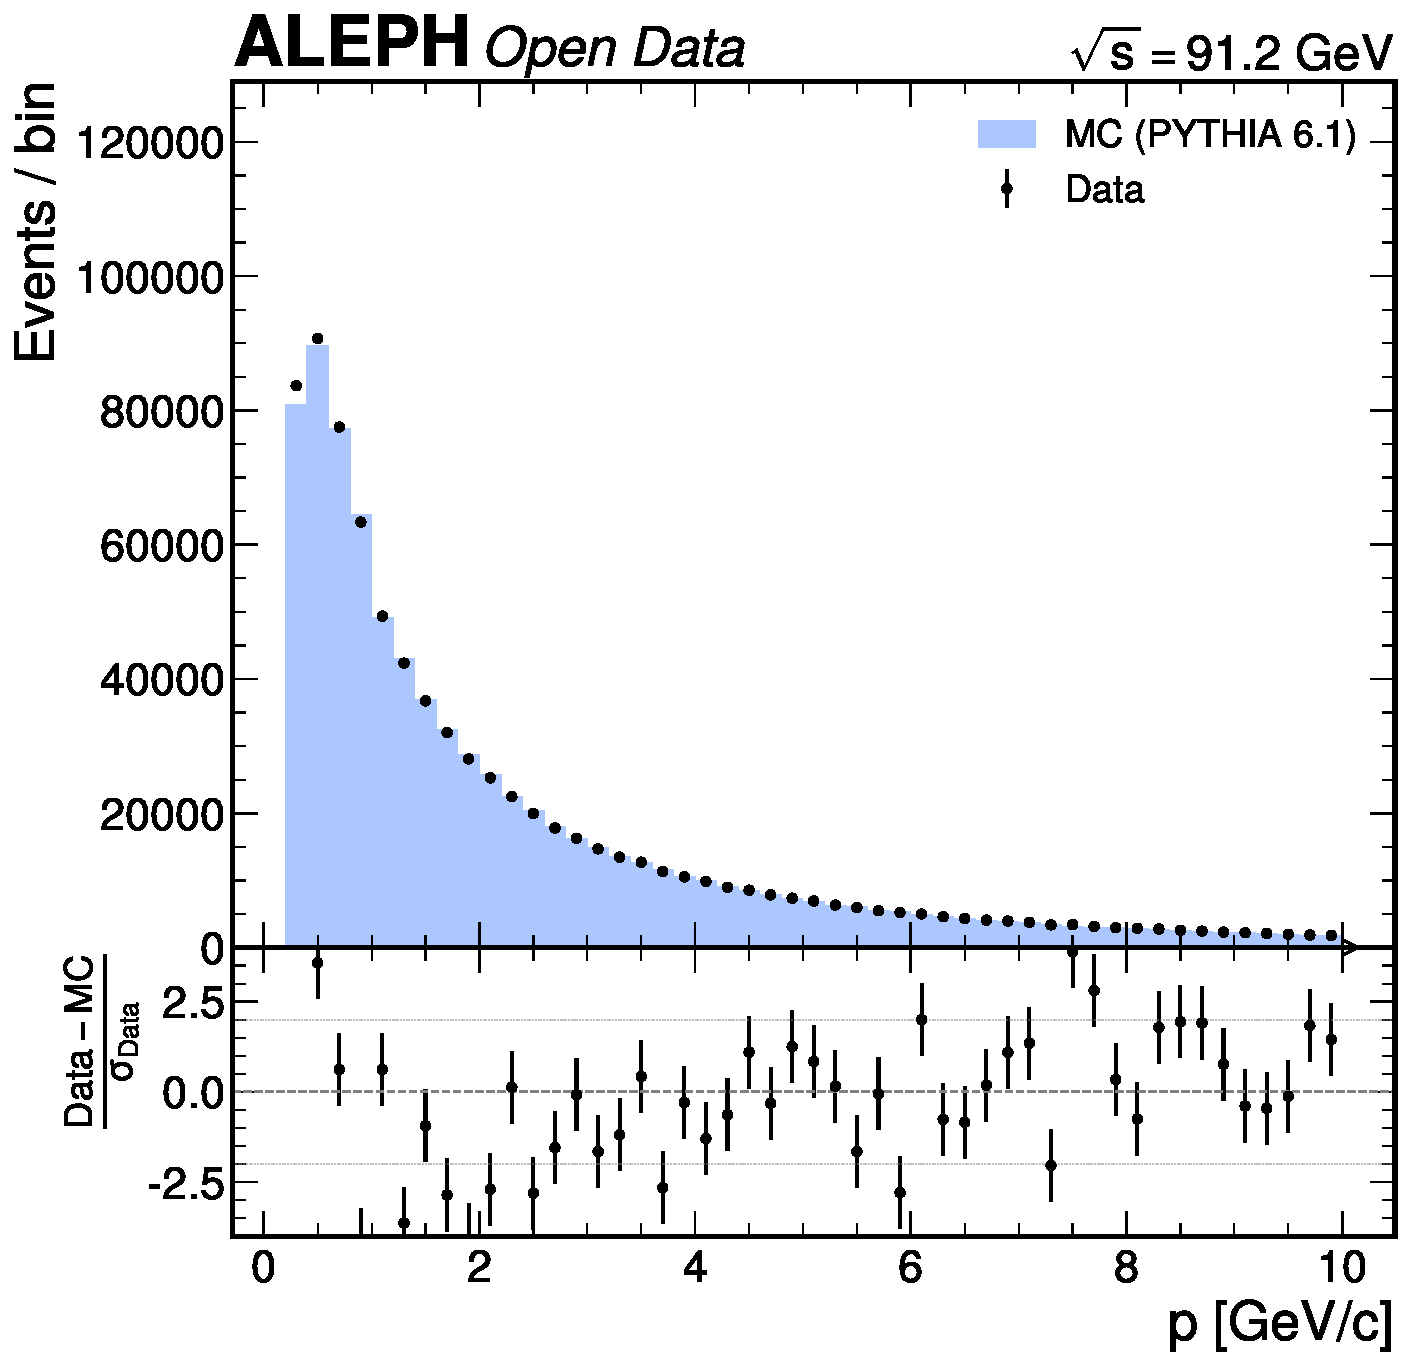
\includegraphics[width=0.47\linewidth]{figures/hugo_pmag_data_mc.pdf}\hspace{1em}%
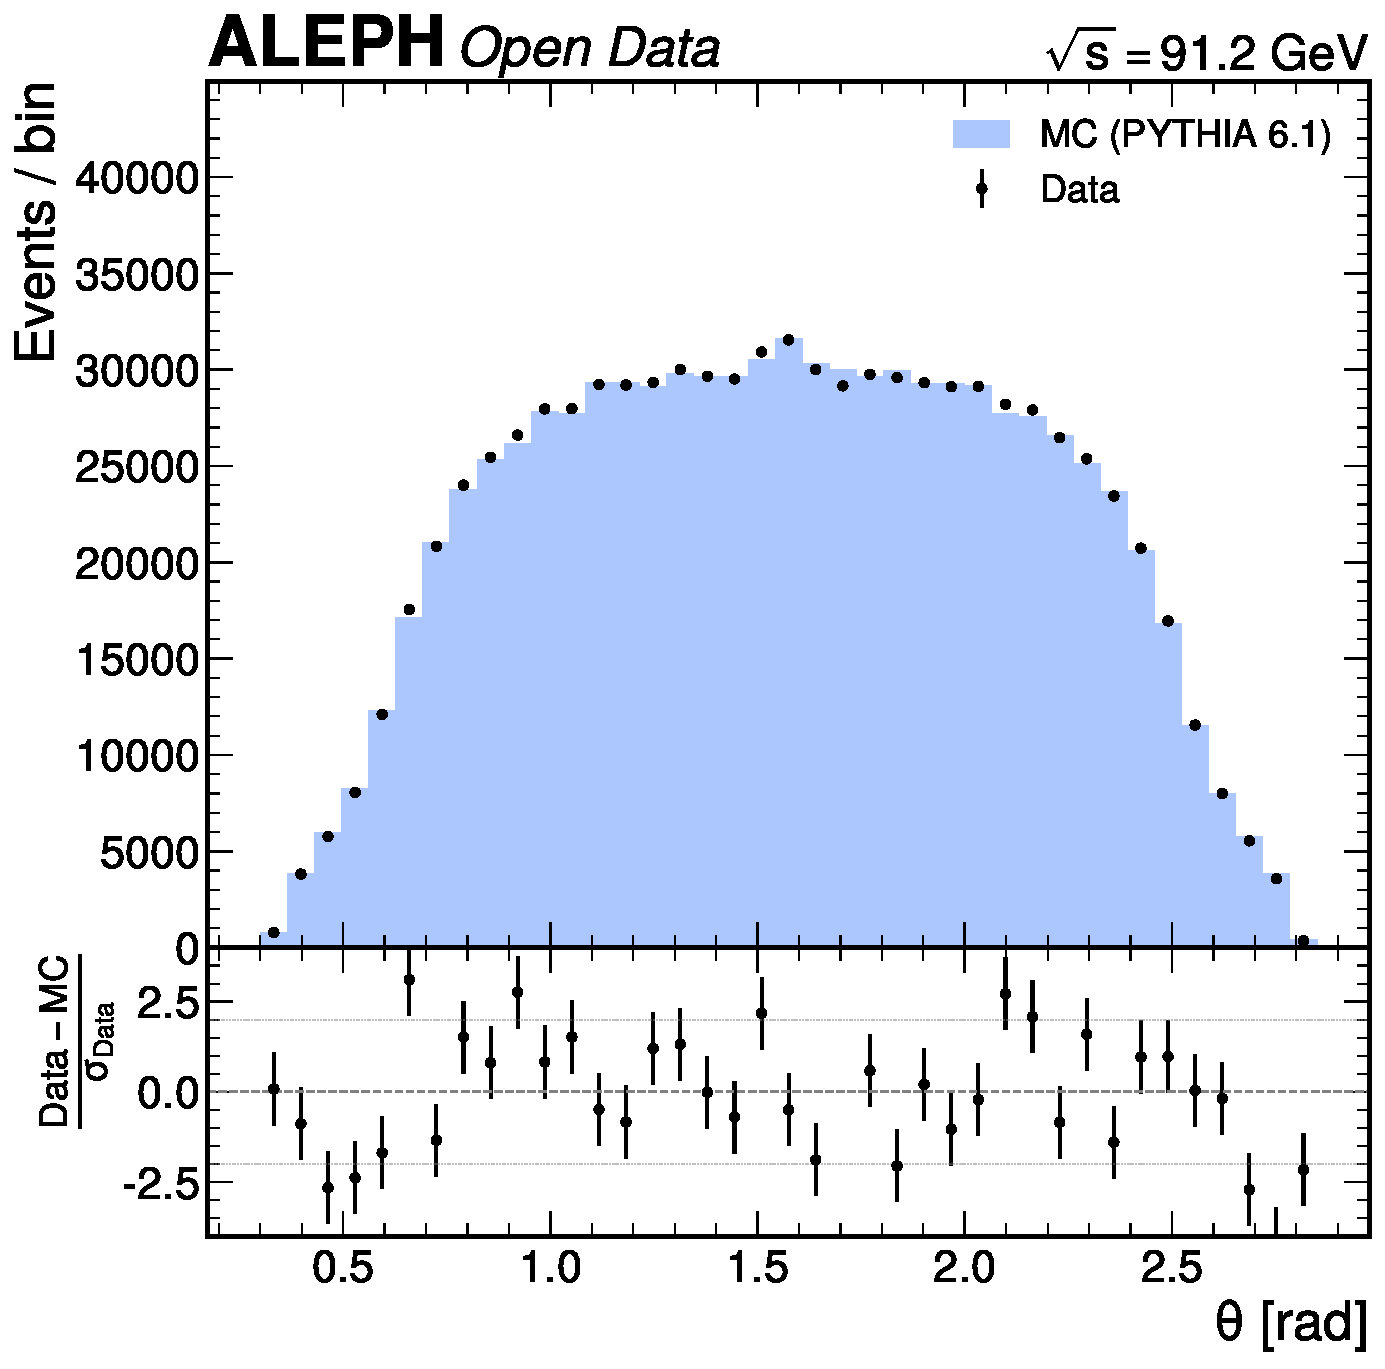
\includegraphics[width=0.47\linewidth]{figures/hugo_theta_data_mc.pdf}
\caption{Data/MC comparison of the charged-particle momentum
  (left) and polar angle $\theta$ (right) distributions after the
  hadronic selection.  The bottom panels show the data/MC ratio.
  Agreement is within $\pm 5\%$ for momentum and $\pm 3\%$ for
  $\theta$ across the full kinematic range, confirming that the MC
  adequately models the detector response for these variables.}
\label{fig:data-mc-p-theta}
\end{figure}

\begin{figure}[htbp]
\centering
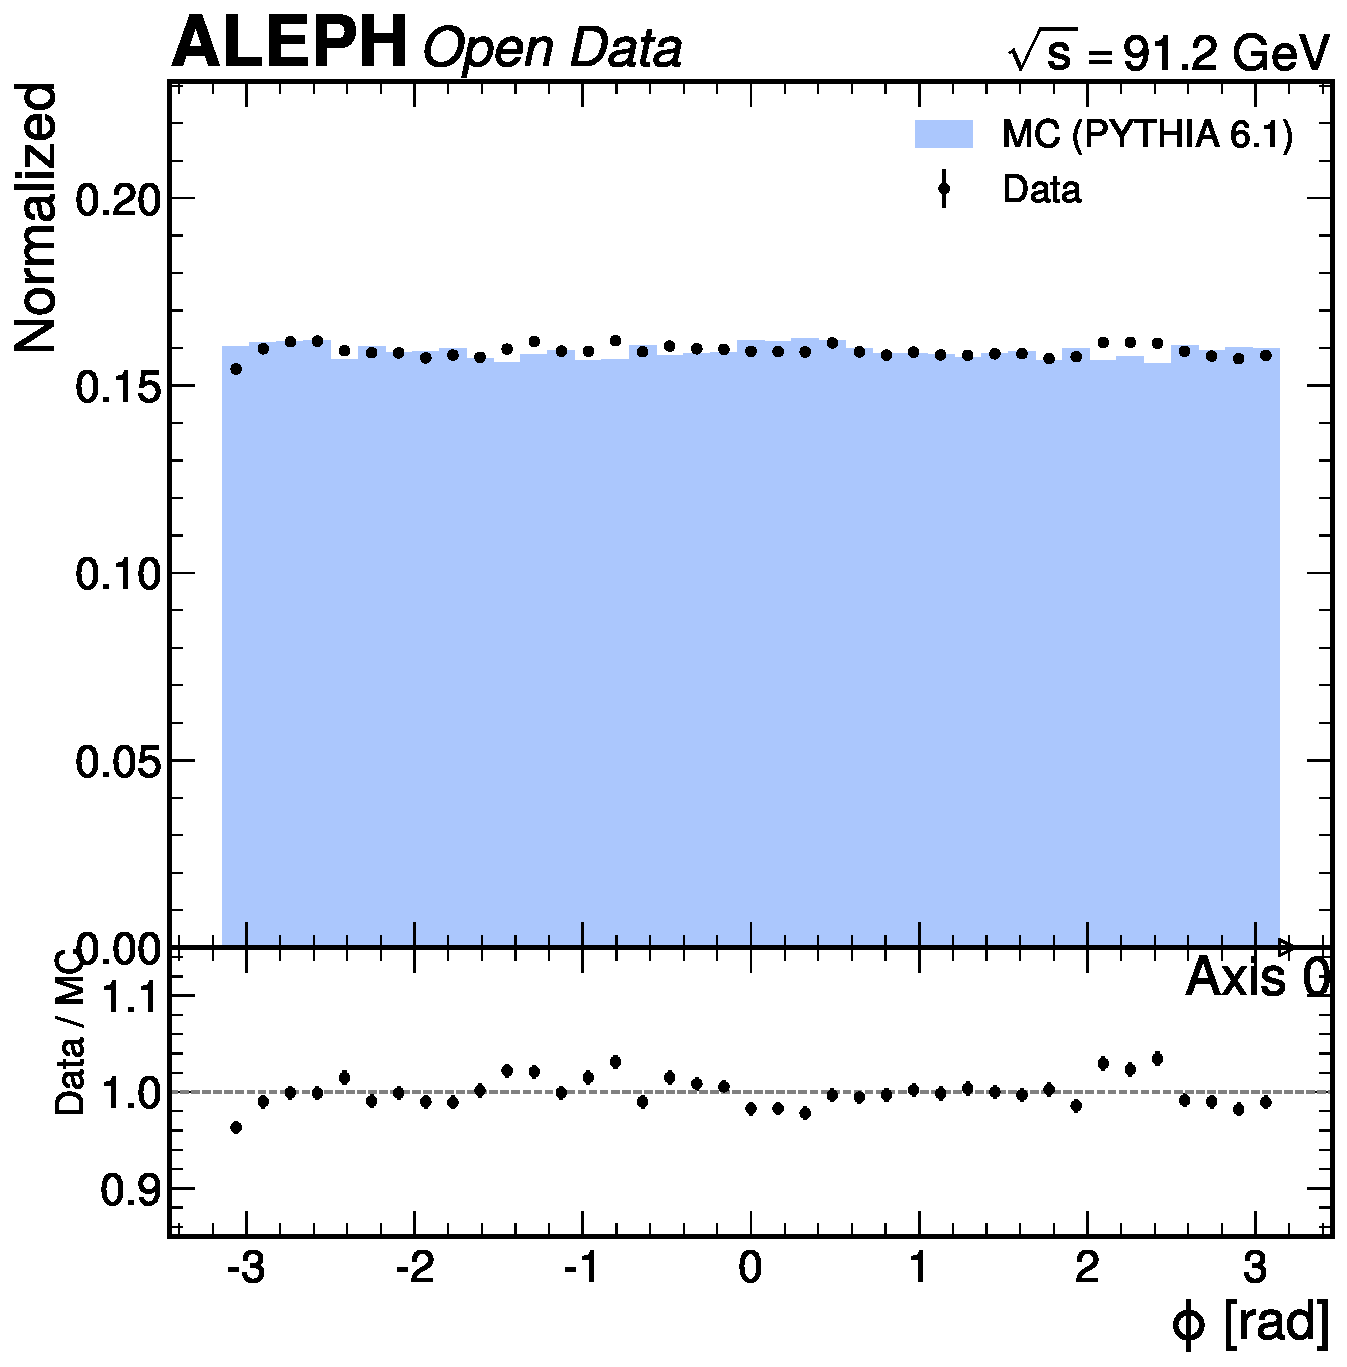
\includegraphics[width=0.47\linewidth]{figures/hugo_phi_data_mc.pdf}\hspace{1em}%
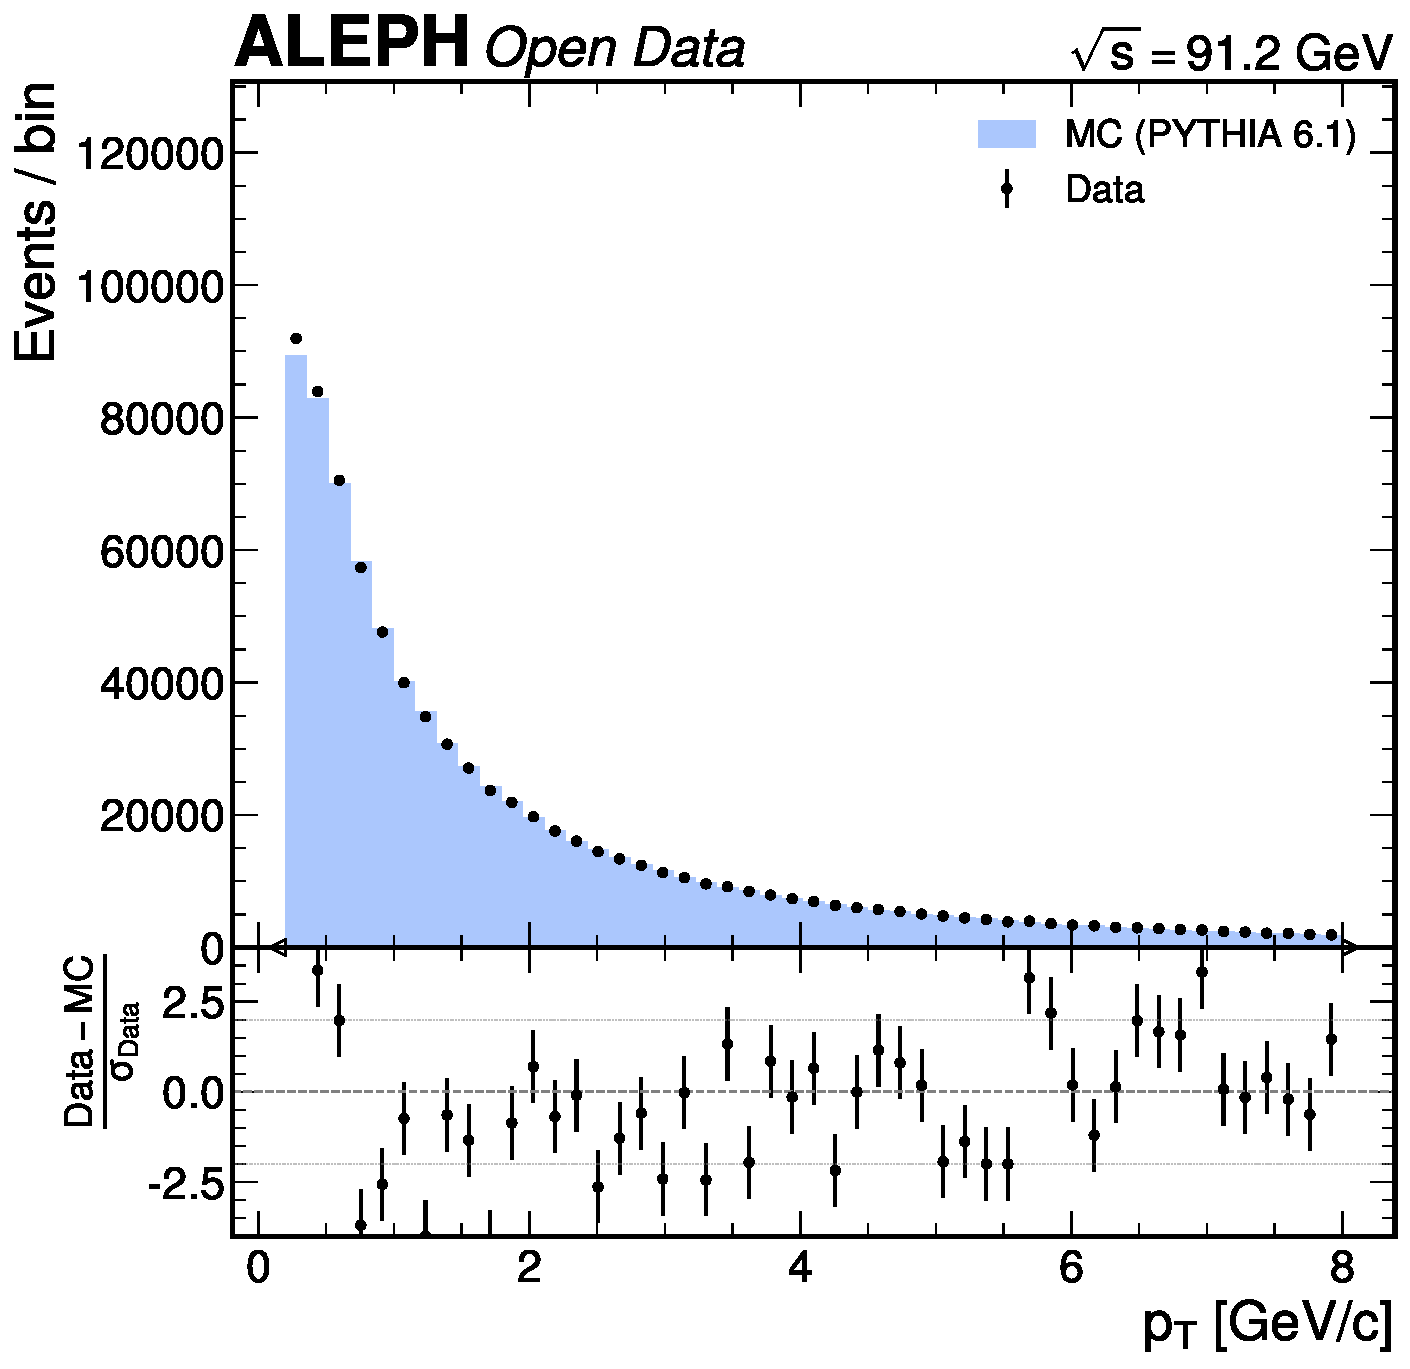
\includegraphics[width=0.47\linewidth]{figures/hugo_pt_data_mc.pdf}
\caption{Data/MC comparison of the azimuthal angle $\phi$ (left) and
  transverse momentum $p_T$ (right).  The $\phi$ distribution is flat
  as expected from azimuthal symmetry, with agreement within $\pm 2\%$.
  The $p_T$ distribution agrees within $\pm 5\%$.}
\label{fig:data-mc-phi-pt}
\end{figure}

\begin{figure}[htbp]
\centering
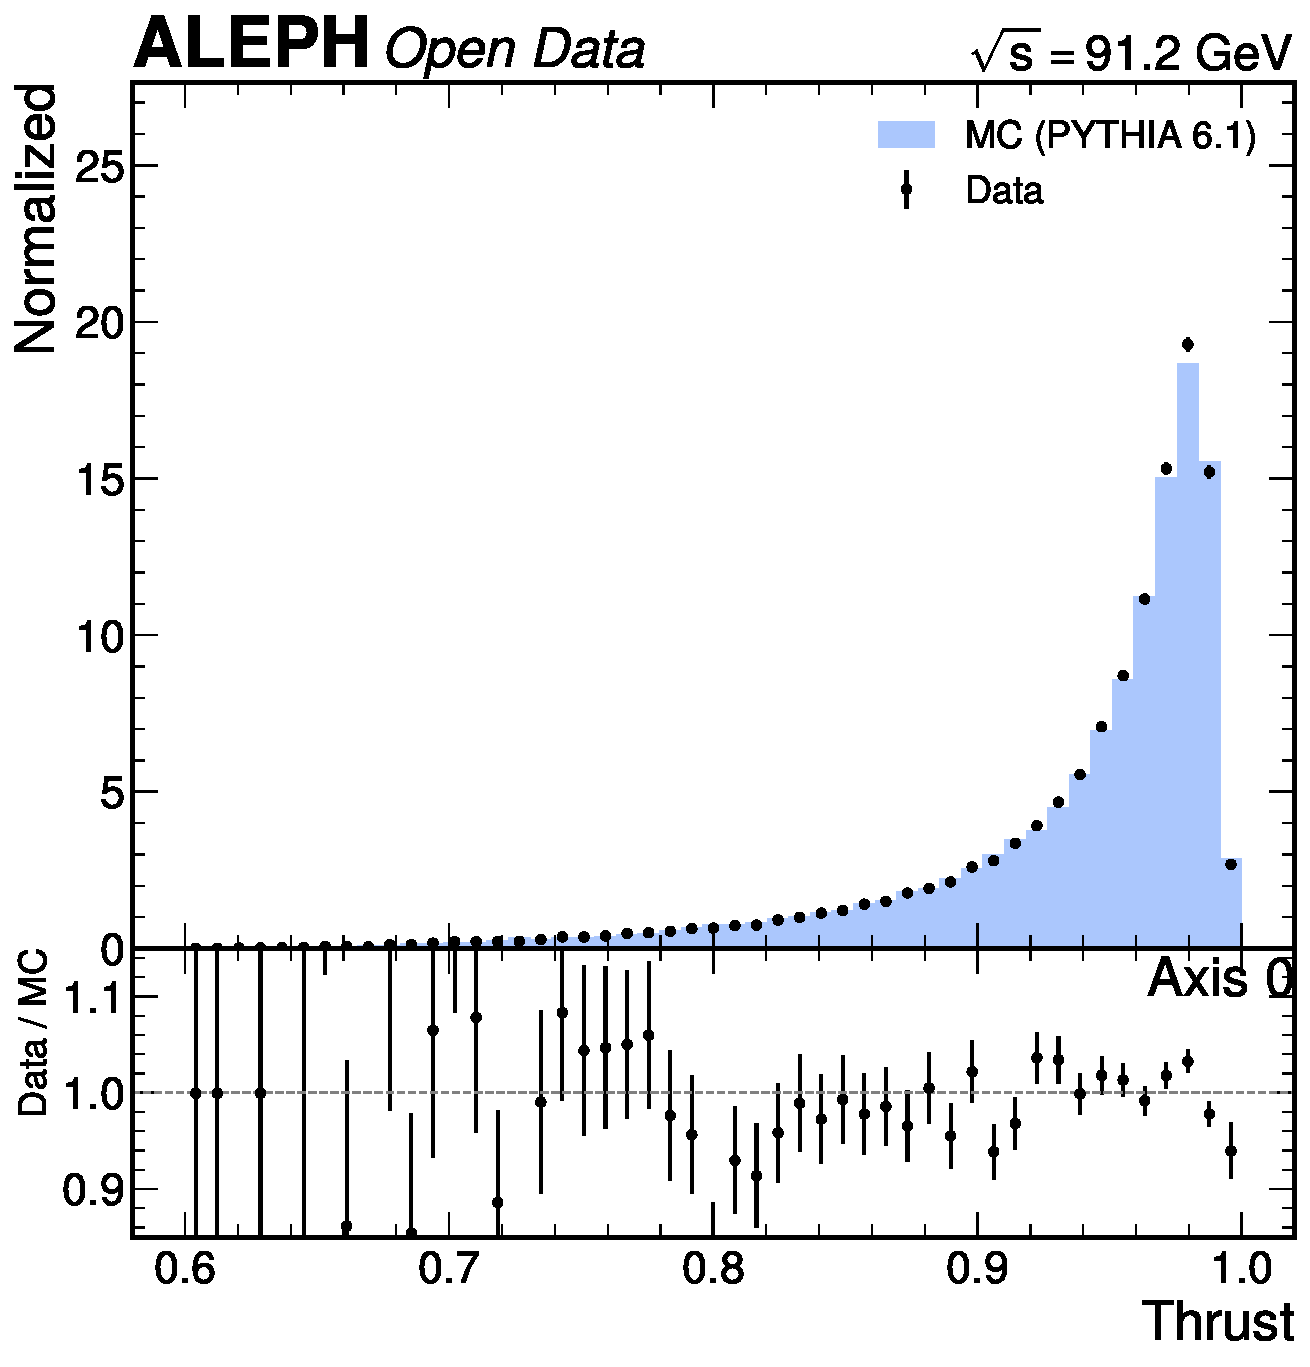
\includegraphics[width=0.47\linewidth]{figures/hugo_thrust_data_mc.pdf}\hspace{1em}%
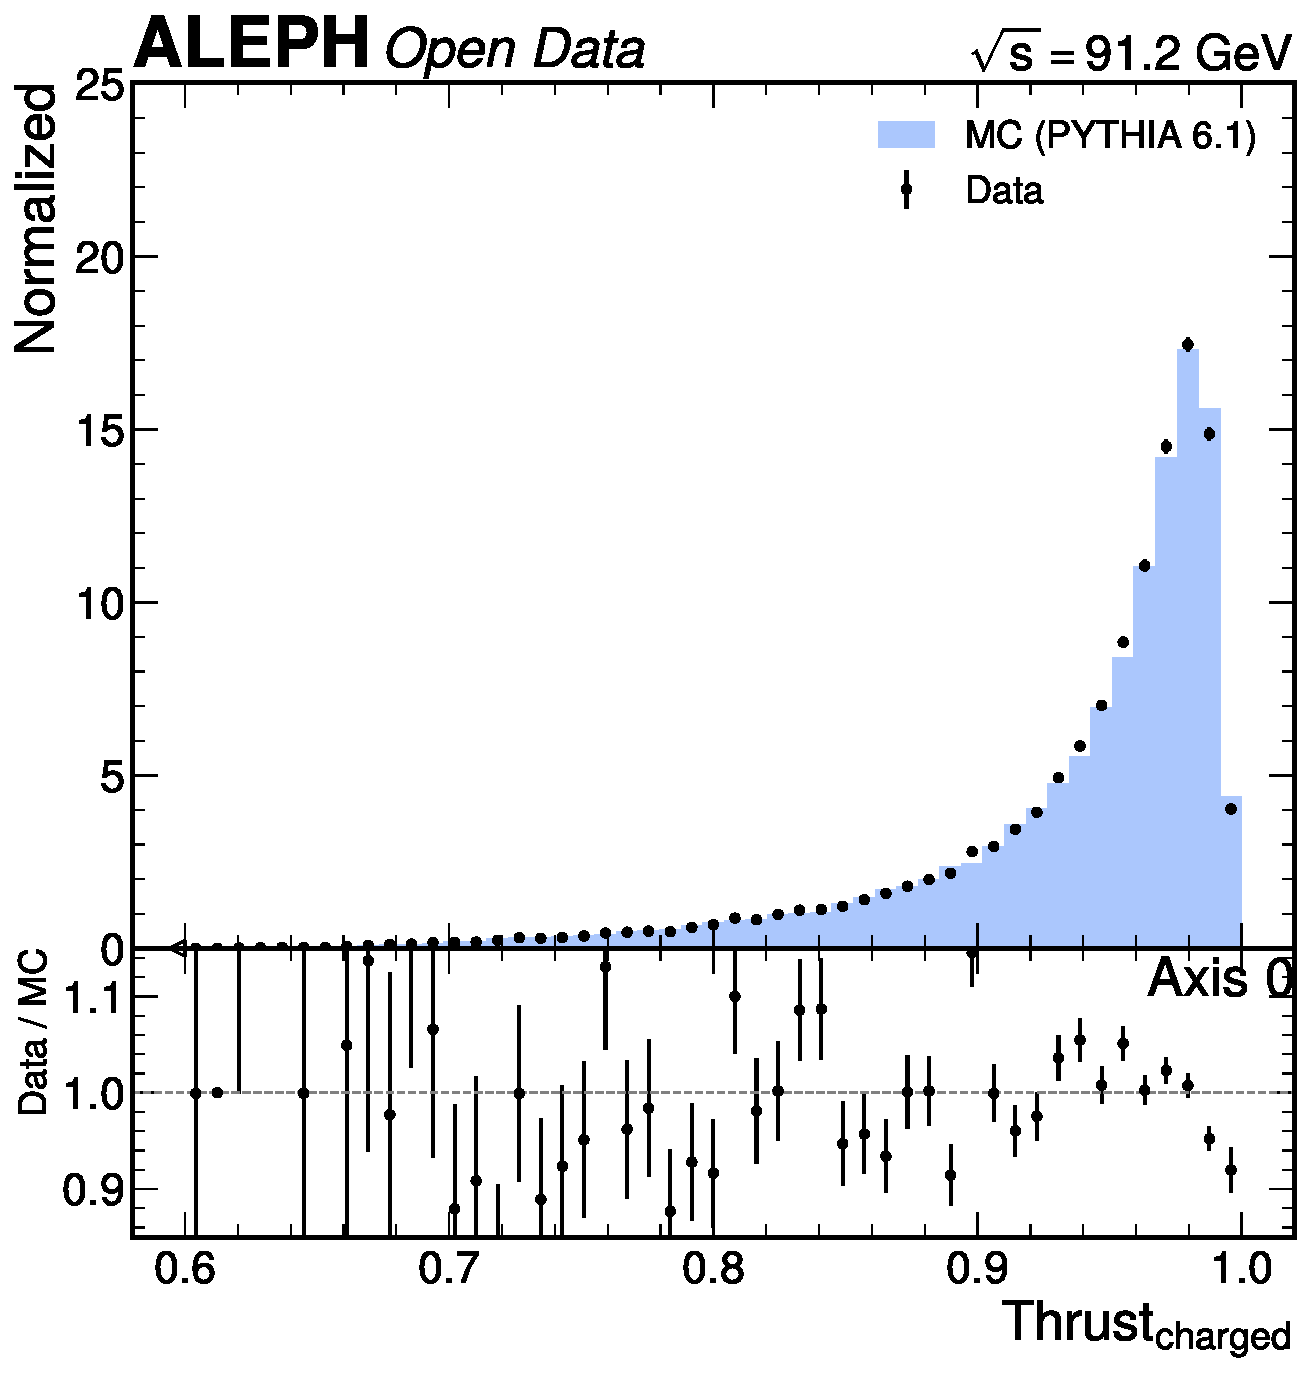
\includegraphics[width=0.47\linewidth]{figures/hugo_thrust_charged_data_mc.pdf}
\caption{Data/MC comparison of the energy-flow thrust (left) and
  charged-only thrust (right).  Both distributions agree within
  $\pm 5\%$.  The thrust cut $T > 0.7$ is indicated; events below
  this threshold are removed.  The difference between energy-flow
  and charged-only thrust ($\sim\!0.15\%$ in the mean) is small but
  systematic, confirming that the pre-computed thrust uses energy-flow
  objects.}
\label{fig:data-mc-thrust}
\end{figure}

\begin{figure}[htbp]
\centering
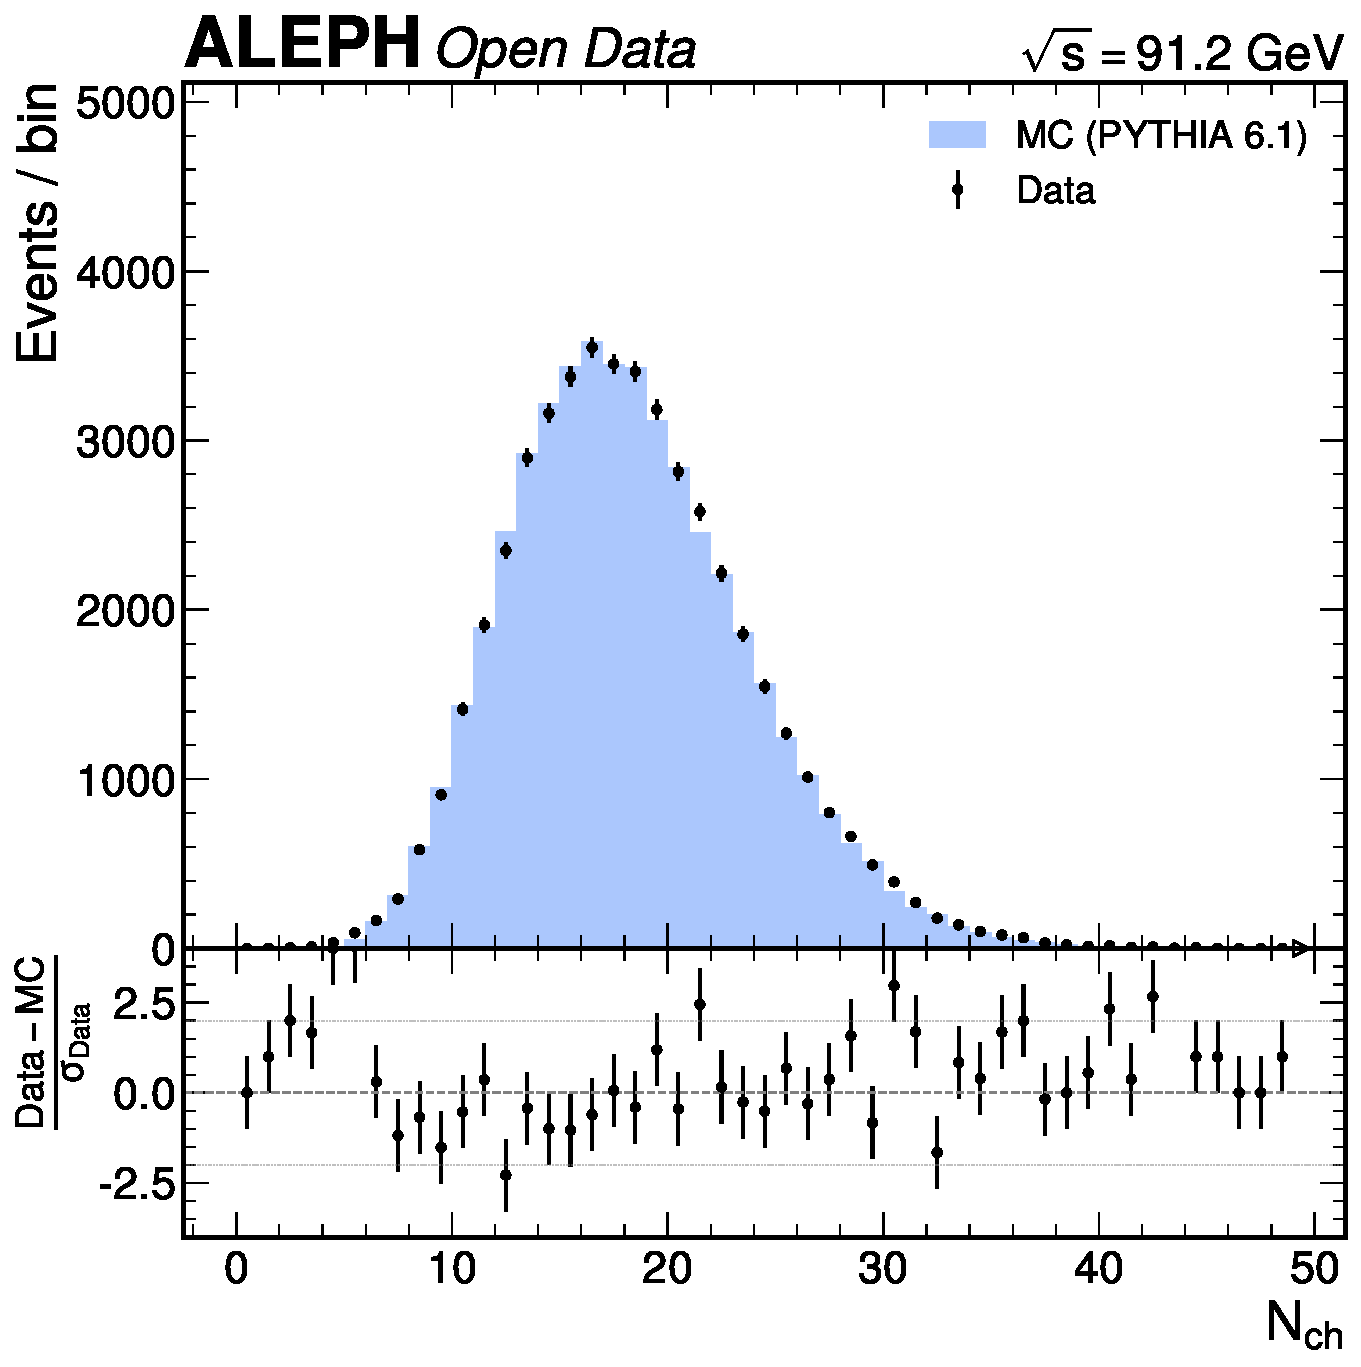
\includegraphics[width=0.47\linewidth]{figures/hugo_nch_data_mc.pdf}\hspace{1em}%
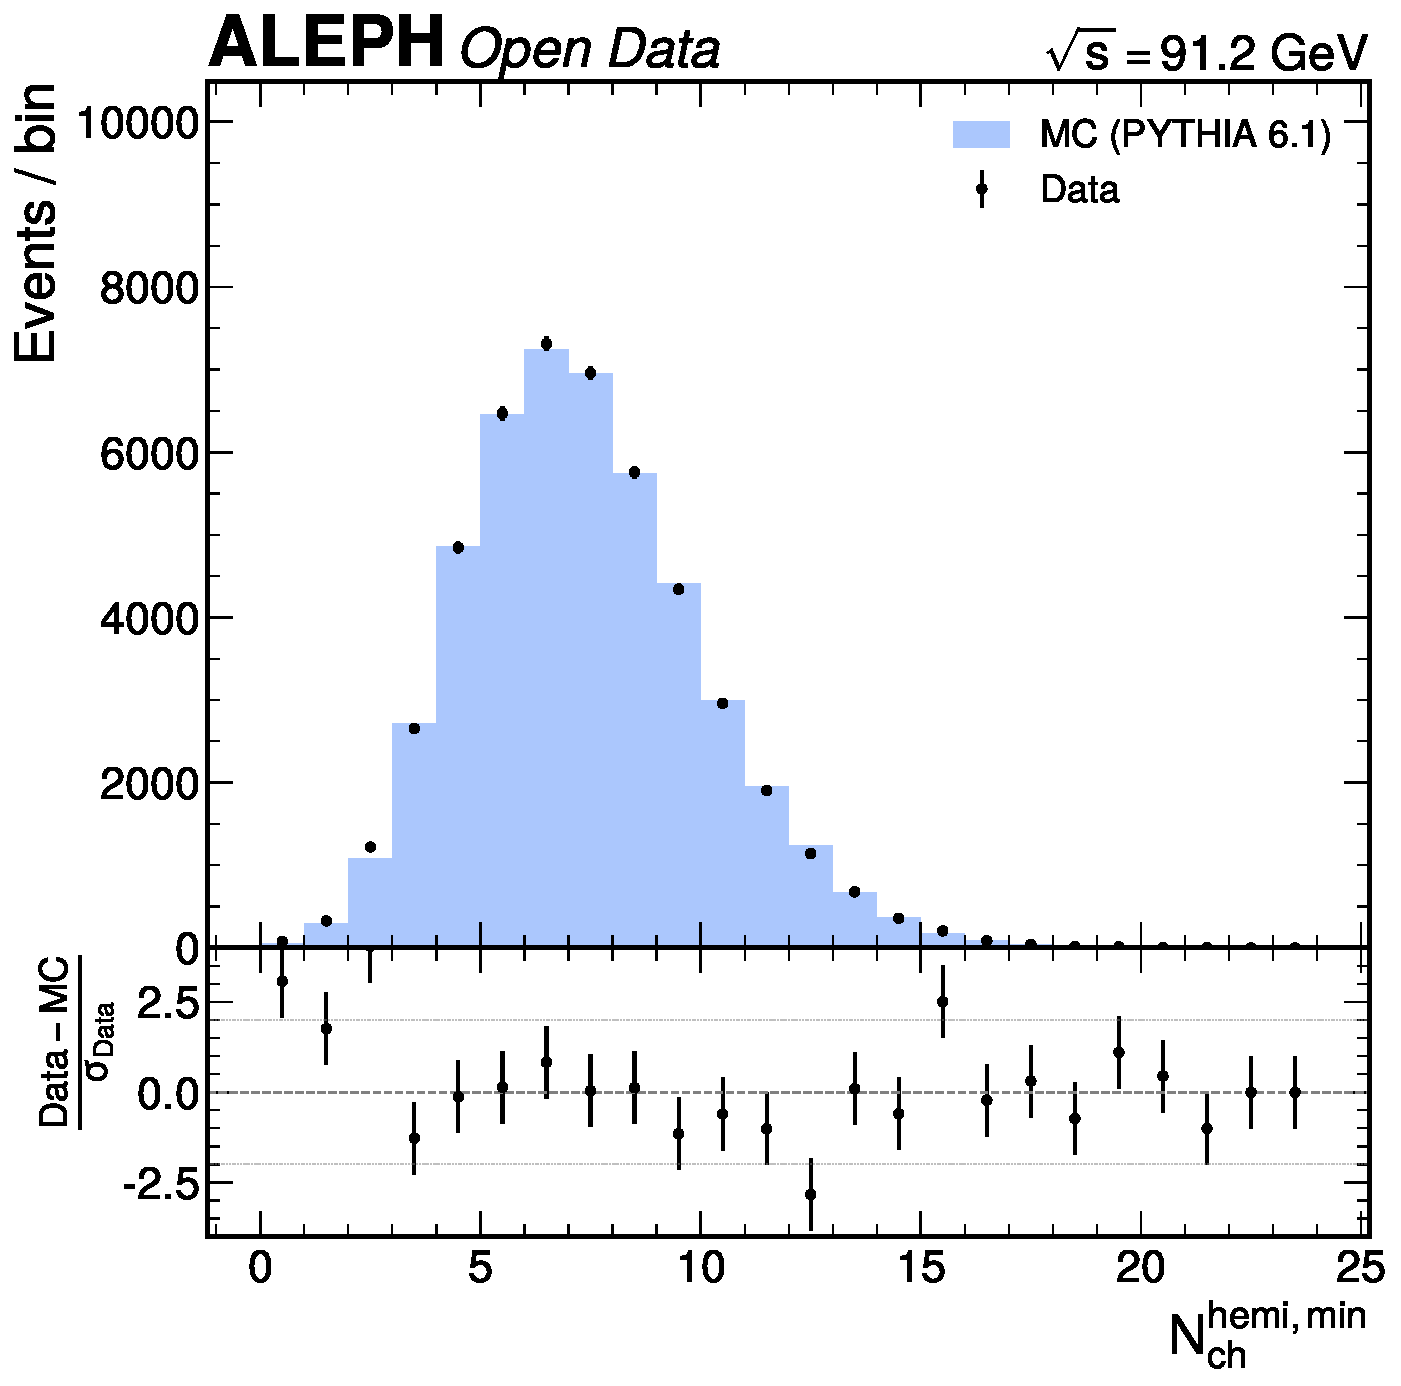
\includegraphics[width=0.47\linewidth]{figures/hugo_hemi_mult_data_mc.pdf}
\caption{Data/MC comparison of the charged multiplicity $N_\text{ch}$
  (left) and the minimum hemisphere multiplicity (right).  Agreement
  is within $\pm 5\%$ for both distributions.  The low-multiplicity
  region ($N_\text{ch} < 10$) is well-modelled, confirming that the
  minimum-track cuts do not introduce data/MC bias.}
\label{fig:data-mc-nch}
\end{figure}

% =====================================================================
% 4. CORRECTIONS / UNFOLDING
% =====================================================================
\section{Corrections}
\label{sec:corrections}

\subsection{Lund plane construction}
\label{sec:lund-construction}

For each selected event, the Lund plane is constructed as follows:
\begin{enumerate}
\item \textbf{Hemisphere splitting:} Selected charged tracks are
  divided into two hemispheres using the pre-computed energy-flow thrust
  axis (TTheta, TPhi) via the sign of $\vec{p} \cdot \hat{n}_T$.
\item \textbf{C/A clustering:} Each hemisphere is clustered using the
  Cambridge/Aachen algorithm~\cite{Dokshitzer:1997in}
  (FastJet~\cite{Cacciari:2011ma} \texttt{ee\_genkt\_algorithm} with
  $p = 0$, $R = 999$, E-scheme recombination).
\item \textbf{Primary declustering:} The clustering tree is followed
  from the fully merged jet, undoing each clustering step.  At each
  step, the harder subjet (larger $p_T$ w.r.t.\ beam axis) is followed.
\item \textbf{Lund coordinates:} For each splitting, $\Delta\theta$ and
  $k_T$ are computed per Eq.~\eqref{eq:kt-dtheta} and mapped to
  $(x, y)$ per Eq.~\eqref{eq:coords}.
\end{enumerate}

The Lund plane construction statistics at each processing level are
summarised in Table~\ref{tbl:lund-stats}.
\begin{table}[htbp]
\centering
\caption{Lund plane construction statistics at each processing level.}
\label{tbl:lund-stats}
\begin{tabular}{lccc}
\toprule
Level & Hemispheres & Splittings & Avg.\ splits/hemi \\
\midrule
Data & 5\,692\,388 & 28\,934\,792 & 5.08 \\
MC reco & 1\,442\,350 & 7\,405\,085 & 5.13 \\
MC gen & 1\,534\,930 & 8\,352\,333 & 5.44 \\
MC genBefore & 1\,936\,712 & 10\,514\,849 & 5.43 \\
\bottomrule
\end{tabular}
\end{table}

The gen-level has $\sim\!6\%$ more splittings per hemisphere than
reco, reflecting track reconstruction losses.  The genBefore and gen
samples have identical splits per hemisphere (5.43 vs 5.44),
confirming that the event selection does not bias the per-hemisphere
splitting rate.

\subsection{Binning}
\label{sec:binning}

The Lund plane is binned in a $10 \times 10$ uniform grid:
\begin{itemize}
\item $\ln(1/\Delta\theta)$: 10 bins from 0 to 5, step 0.5.
\item $\ln(k_T/\text{GeV})$: 10 bins from $-3$ to $+4$, step 0.7.
\item Bin area: $\Delta x \cdot \Delta y = 0.5 \times 0.7 = 0.35$.
\item 100 total bins; 58 populated (42 depopulated at kinematic
  boundaries).
\end{itemize}

The binning was validated during Phase~2 exploration, as shown in
Figure~\ref{fig:binning}:
the migration fraction $|N_\text{reco} - N_\text{gen}|/N_\text{reco}$
is below 30\% in 93 of 100 bins, and the bin population exceeds 100
data entries and 50 MC entries in all populated bins at full statistics.

\begin{figure}[htbp]
\centering
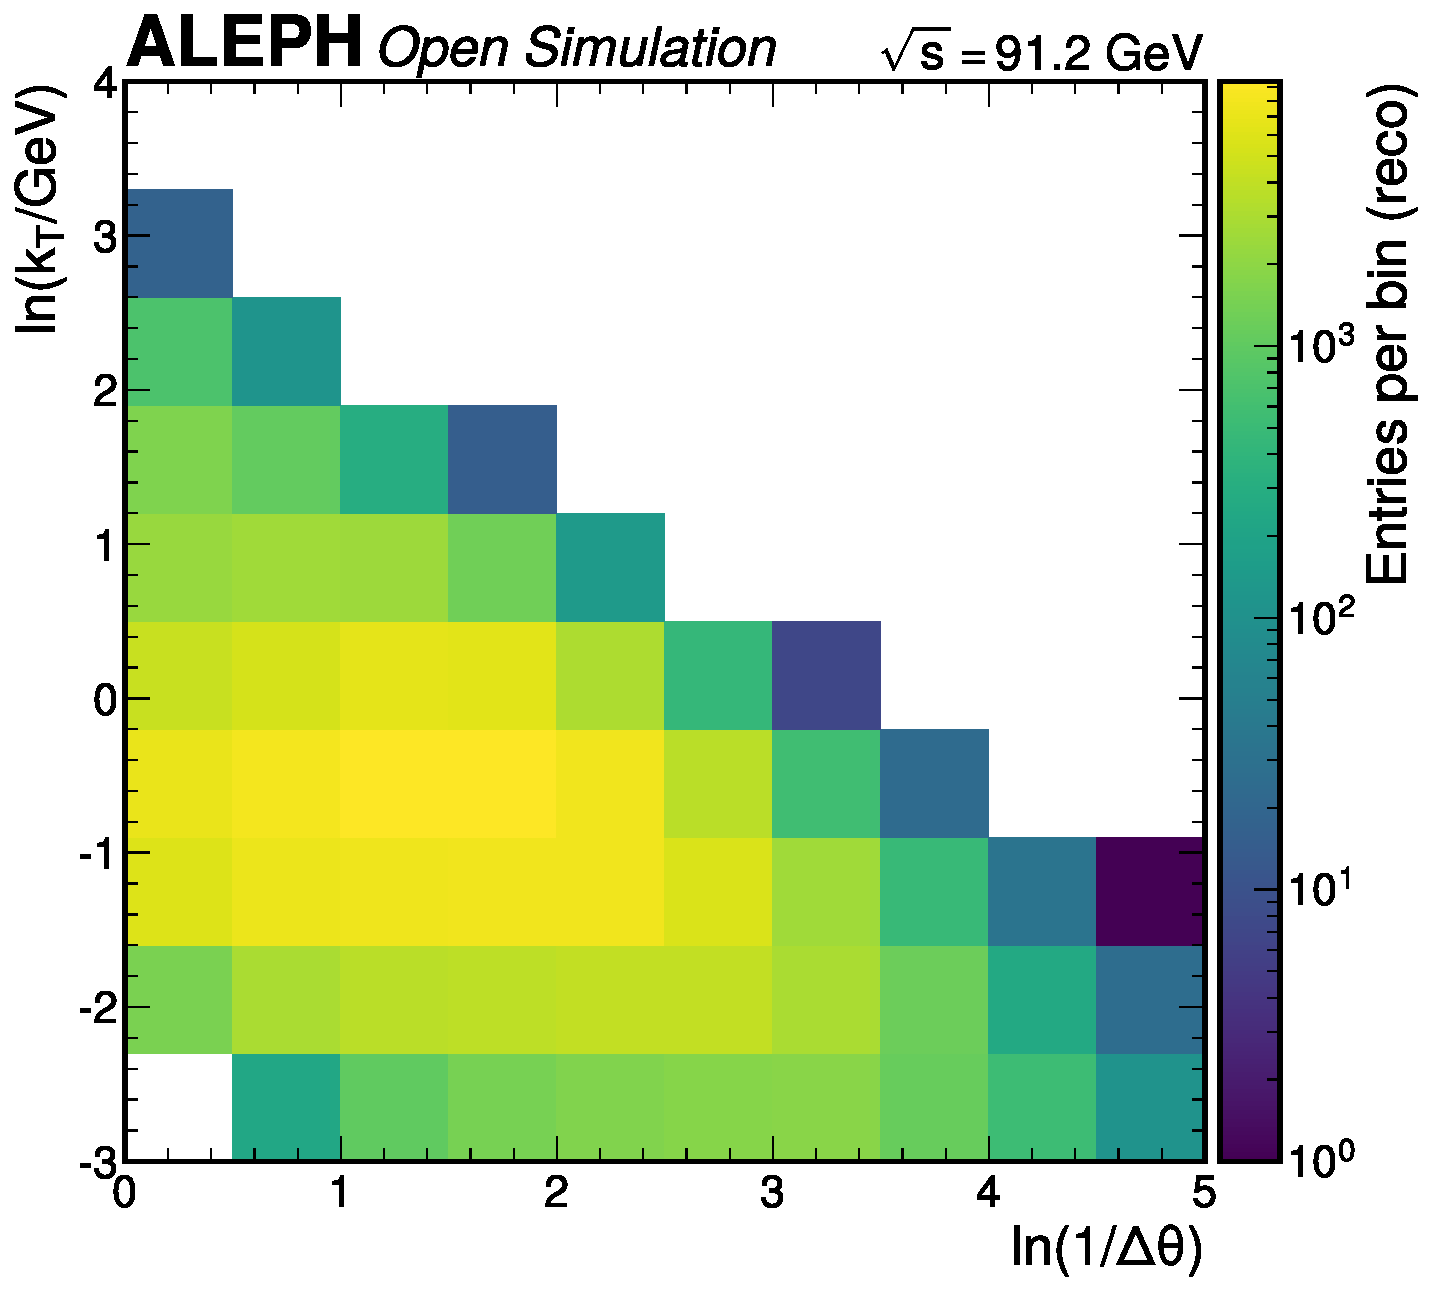
\includegraphics[width=0.47\linewidth]{figures/hugo_bin_population_reco.pdf}\hspace{1em}%
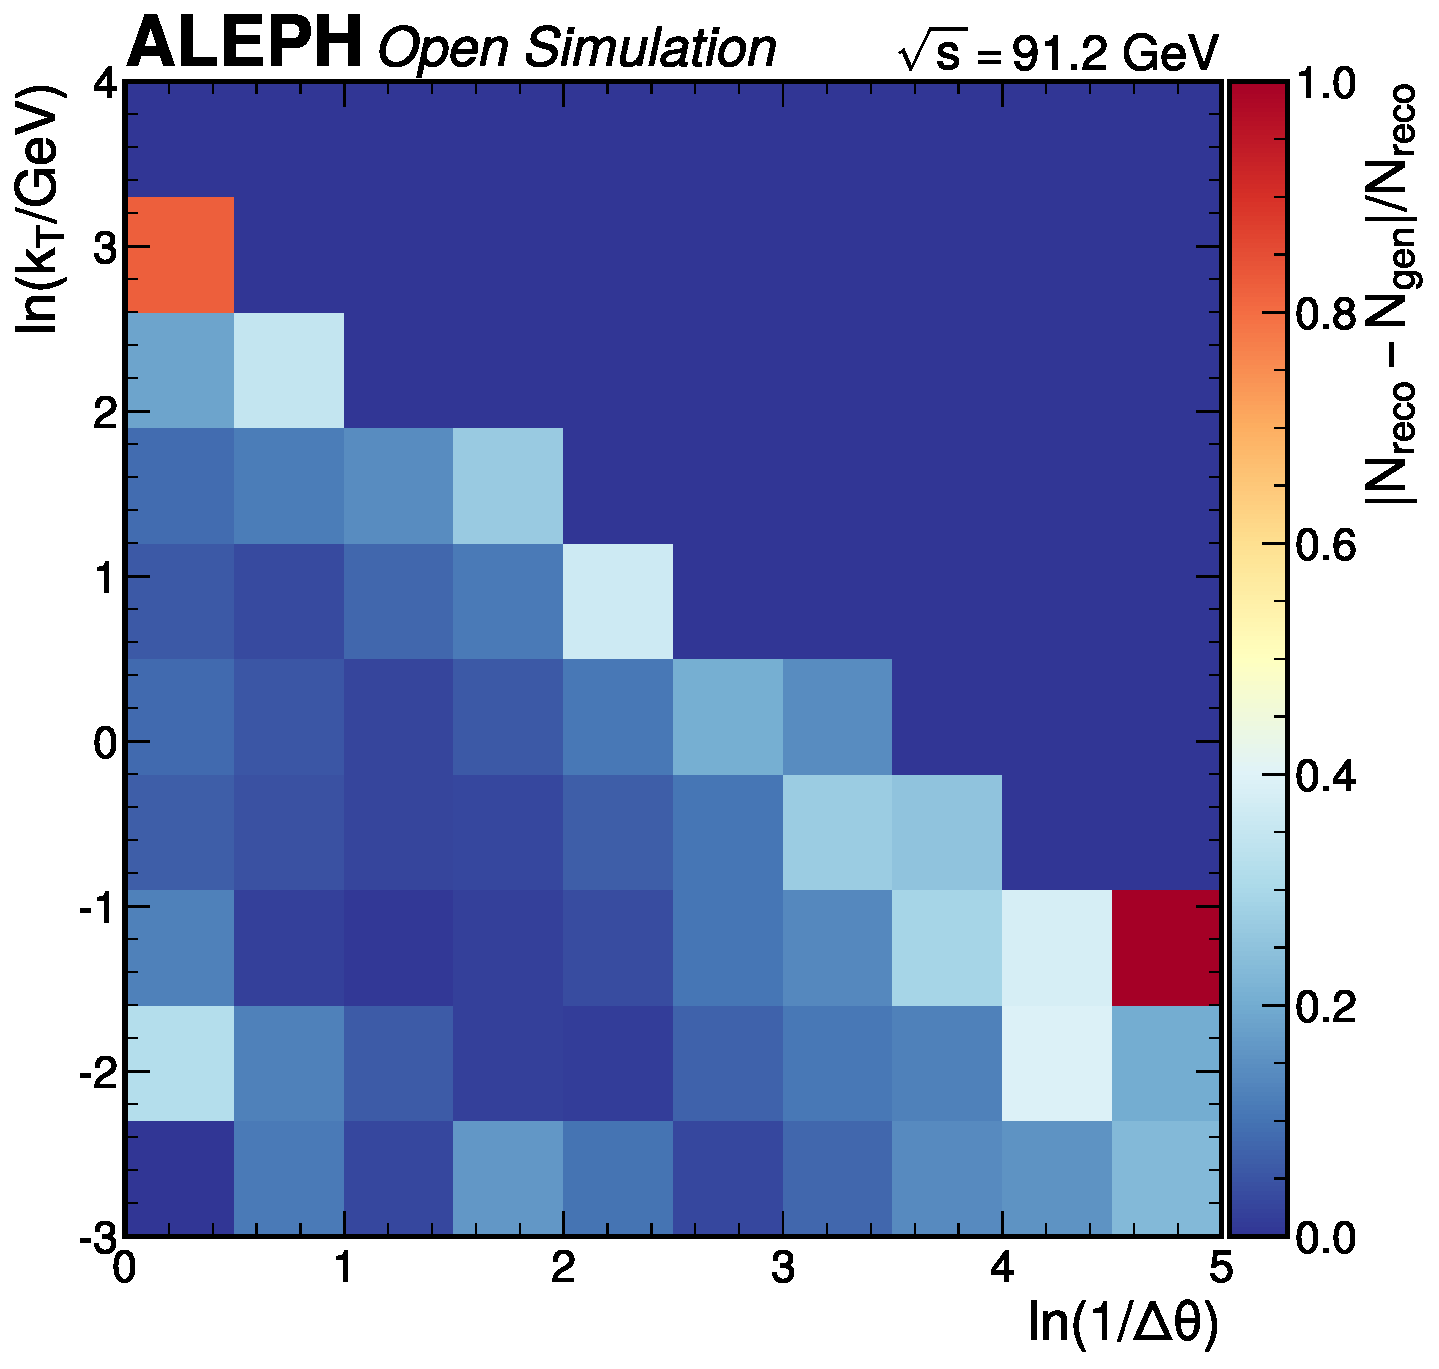
\includegraphics[width=0.47\linewidth]{figures/hugo_migration_fraction.pdf}
\caption{Bin population at reco level for the $10 \times 10$ binning
  (left) and migration fraction $|N_\text{reco} - N_\text{gen}|/N_\text{reco}$
  per bin (right).  The kinematic boundary naturally depopulates the
  upper-left and lower-right corners.  The mean migration fraction
  is 14\%, with only 7 bins exceeding 30\% (all at boundaries).
  These figures confirm that the uniform binning provides adequate
  resolution for the bin-by-bin correction method.}
\label{fig:binning}
\end{figure}

\subsection{Bin-by-bin correction (primary method)}
\label{sec:bbb}

The correction factor for each bin $(i,j)$ of the Lund plane is
defined as
\begin{equation}
  C(i,j) = \frac{N_\text{genBefore}(i,j)}{N_\text{reco}(i,j)}\,,
  \label{eq:correction}
\end{equation}
where $N_\text{genBefore}(i,j)$ is the number of primary splittings at
generator level from all events in the \texttt{tgenBefore} tree (before
event selection), and $N_\text{reco}(i,j)$ is the count at reconstruction
level from selected events (Eq.~\eqref{eq:correction}).  This combined
correction factor
simultaneously accounts for:
\begin{itemize}
\item Detector resolution and track reconstruction effects
  (migration between bins).
\item Event-level selection efficiency ($\sim\!79\%$).
\item Track-level reconstruction efficiency.
\end{itemize}

The corrected Lund plane density in each bin is then given by
Eq.~\eqref{eq:corrected-density}:
\begin{equation}
  \rho_\text{corrected}(i,j) =
  \frac{N_\text{reco}(i,j) \cdot C(i,j)}
       {N_\text{jet}^\text{genBefore}\;\Delta x\;\Delta y}
  = \frac{N_\text{genBefore}(i,j)}
         {N_\text{jet}^\text{genBefore}\;\Delta x\;\Delta y}\,,
  \label{eq:corrected-density}
\end{equation}
where $N_\text{jet}^\text{genBefore} = 1\,936\,712$ hemispheres and
$\Delta x \cdot \Delta y = 0.35$ is the bin area.
Table~\ref{tbl:correction-stats} summarises the correction factor
statistics across the 58 populated bins.

\begin{table}[htbp]
\centering
\caption{Summary statistics of the bin-by-bin correction factors
  $C(i,j)$ across the 58 populated bins.}
\label{tbl:correction-stats}
\begin{tabular}{lc}
\toprule
Statistic & Value \\
\midrule
Mean & 1.680 \\
Median & 1.468 \\
Minimum & 1.166 \\
Maximum & 6.667 \\
Bins with $C > 2$ & 4 \\
Bins with $N_\text{reco} = 0$ & 42 / 100 \\
\bottomrule
\end{tabular}
\end{table}

The median correction of 1.47 is consistent with the event selection
efficiency correction ($\sim\!1/0.79 = 1.27$) plus detector effects.
Only 4 bins at the kinematic boundaries have $C > 2$.
The spatial distribution of the correction factors across the Lund plane
is shown in Figure~\ref{fig:correction-map}.

\begin{figure}[htbp]
\centering
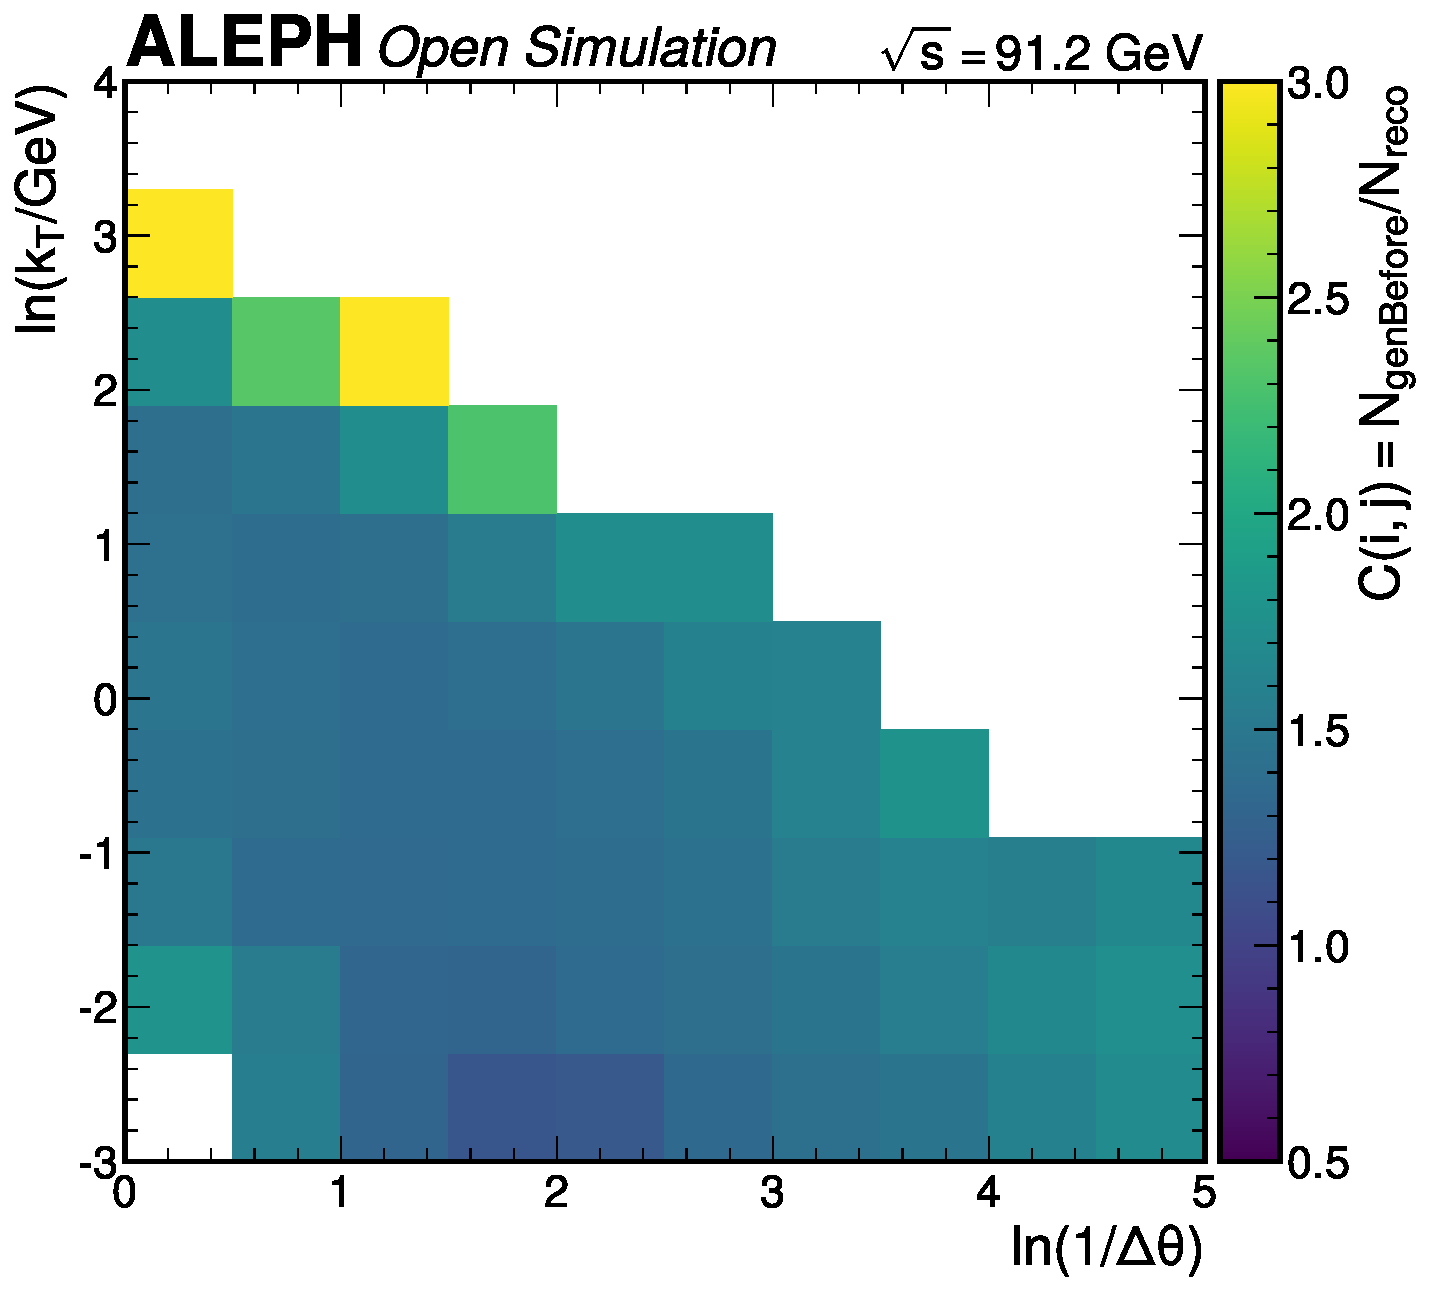
\includegraphics[width=0.55\linewidth]{figures/ingrid_correction_factor_map.pdf}
\caption{Bin-by-bin correction factor map $C(i,j) = N_\text{genBefore}/N_\text{reco}$
  across the Lund plane.  The correction ranges from approximately
  1.2 to 3.0, with a median value of 1.47 in the populated region.
  The minimum value of 1.17 reflects the $\sim\!79\%$ event selection
  efficiency ($1/0.79 \approx 1.27$), with additional contributions from
  detector resolution effects.  Even in the densely populated core the
  correction is typically 1.3--1.5, increasing further at the kinematic
  boundaries where detector effects and bin migration are larger.
  Only 4 bins at the kinematic boundaries have $C > 2$.  This map is
  the central input to the measurement: multiplicative application to
  the data reco-level counts yields the corrected particle-level density.}
\label{fig:correction-map}
\end{figure}

\subsection{Efficiency map}
\label{sec:efficiency}

The event selection efficiency per bin (Eq.~\eqref{eq:efficiency}) is
\begin{equation}
  \varepsilon(i,j) = \frac{N_\text{gen}(i,j)}{N_\text{genBefore}(i,j)}\,,
  \label{eq:efficiency}
\end{equation}
with a mean of 0.731 across populated bins and range $[0, 0.9]$.
Figure~\ref{fig:efficiency-diagonal} shows the efficiency map and the
diagonal fraction across the Lund plane.

\begin{figure}[htbp]
\centering
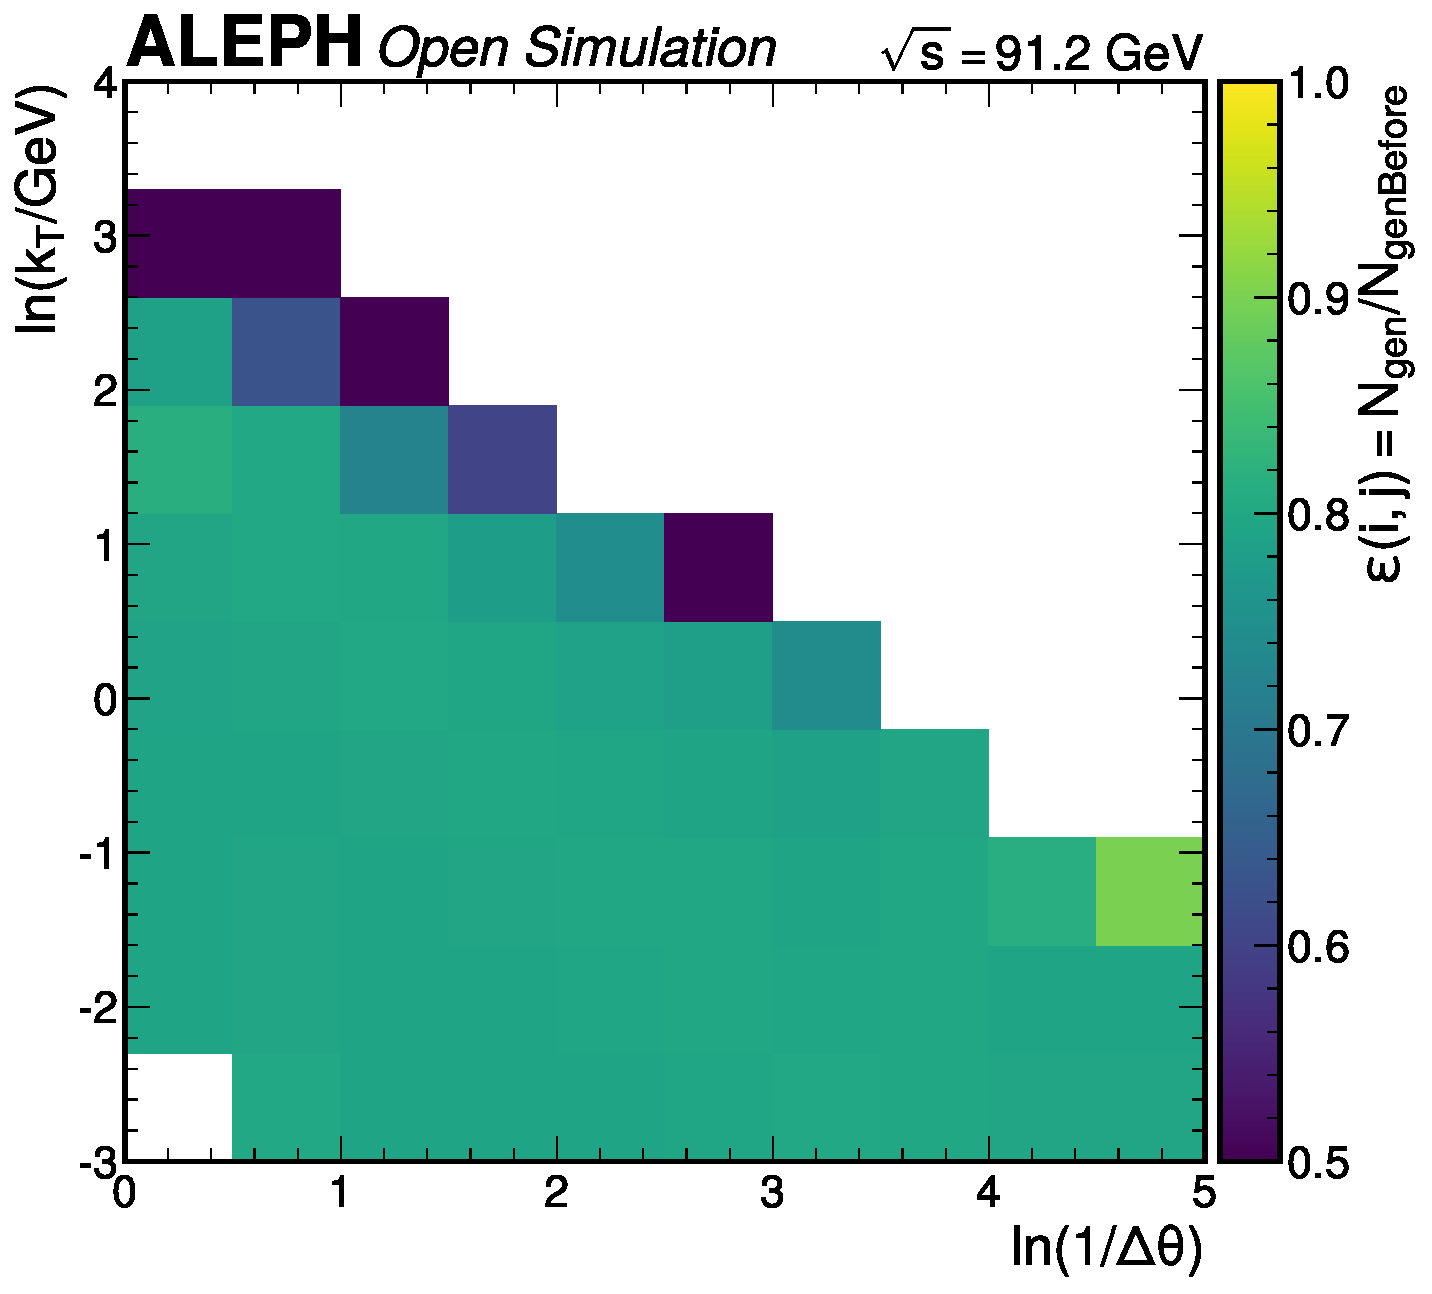
\includegraphics[width=0.47\linewidth]{figures/ingrid_efficiency_map.pdf}\hspace{1em}%
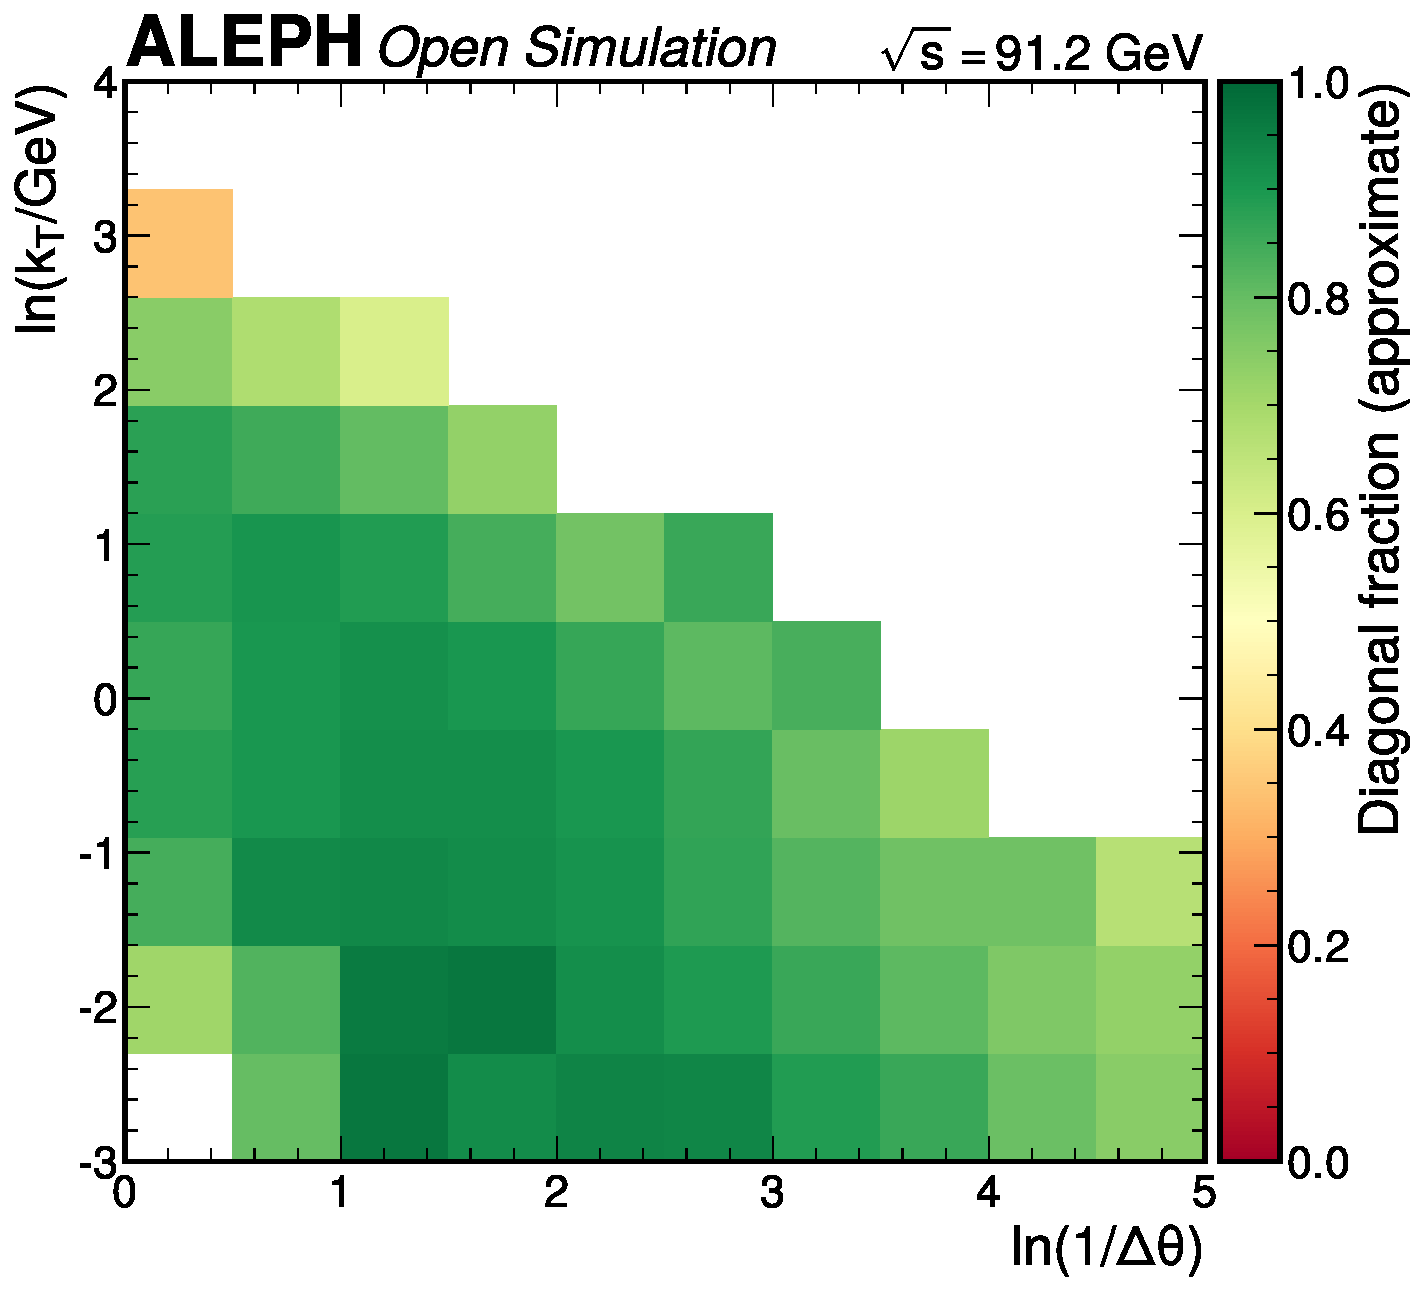
\includegraphics[width=0.47\linewidth]{figures/ingrid_diagonal_fraction_map.pdf}
\caption{Event selection efficiency $\varepsilon(i,j)$ (left) and
  diagonal fraction (right) across the Lund plane.  The efficiency is
  lowest at the kinematic boundaries where the event selection removes
  poorly contained geometries.  The diagonal fraction (fraction of
  splittings that remain in the same bin between gen and reco) has a
  mean of 0.836, with 57 of 58 populated bins above 0.5, confirming
  that the bin-by-bin correction method is well-suited to this observable.}
\label{fig:efficiency-diagonal}
\end{figure}

\subsection{Closure test}
\label{sec:closure}

The closure test applies the correction factors to the MC reco-level
counts and compares to the genBefore truth density.  When the
corrections are derived and applied to the \emph{same} MC sample,
the result is an algebraic identity:
$N_\text{reco} \times C = N_\text{reco} \times
(N_\text{genBefore}/N_\text{reco}) = N_\text{genBefore}$, yielding
$\chi^2/\text{ndf} = 0.0/58$ and $p = 1.0$.  This is the expected
behaviour and confirms the implementation is correct, but does not
validate the method's resolving power.  The genuine validation is
provided by the split-sample closure (Section~\ref{sec:split-closure}).

\subsection{Split-sample closure test}
\label{sec:split-closure}

The MC is split into half~A (files 1--20) and half~B (files 21--40).
Correction factors are derived from half~A: $C_A = N_\text{genBefore}^A
/ N_\text{reco}^A$.  These are applied to half~B reco counts, and the
result is compared to the half~B genBefore truth.

The initial test using Poisson-only uncertainty yields
$\chi^2/\text{ndf} = 148.9/58 = 2.57$ ($p = 6.2 \times 10^{-10}$),
which fails the $p > 0.05$ criterion.  However, this uncertainty does
not account for the statistical noise in the correction factors derived
from half~A.  Three remediations were performed:

\subsubsection{Remediation 1: Combined uncertainty}

The combined uncertainty accounts for both Poisson noise on the truth
counts and the statistical uncertainty on the correction factors:
\begin{equation}
  \sigma^2_\text{combined} = N_\text{truth}^B +
  \left(N_\text{reco}^B \cdot C_A\right)^2
  \left(\frac{1}{N_\text{reco}^A} + \frac{1}{N_\text{genBefore}^A}\right).
  \label{eq:combined-sigma}
\end{equation}
Result: $\chi^2/\text{ndf} = 40.71/58 = 0.70$ ($p = 0.96$).  Pull
mean $= -0.14$, pull std $= 0.83$.  \textbf{PASSES.}

\subsubsection{Remediation 2: 30/10 file split}

Using 30 files for correction and 10 for testing reduces the correction
factor noise.  With combined uncertainty:
$\chi^2/\text{ndf} = 53.87/58 = 0.93$ ($p = 0.63$).  \textbf{PASSES.}

\subsubsection{Remediation 3: Boundary bin exclusion}

Excluding 2 bins with $C > 3$: core combined
$\chi^2/\text{ndf} = 39.21/56 = 0.70$ ($p = 0.96$).  \textbf{PASSES.}

\medskip

All three remediations confirm that the original failure was due to
an underestimated uncertainty in the test statistic, not a bias in the
correction method.  The combined uncertainty (Remediation~1) is adopted
as the standard.  The split-sample closure projections are shown in
Figure~\ref{fig:split-closure}, and the corresponding pull distribution
in Figure~\ref{fig:closure-pulls}.

\begin{figure}[htbp]
\centering
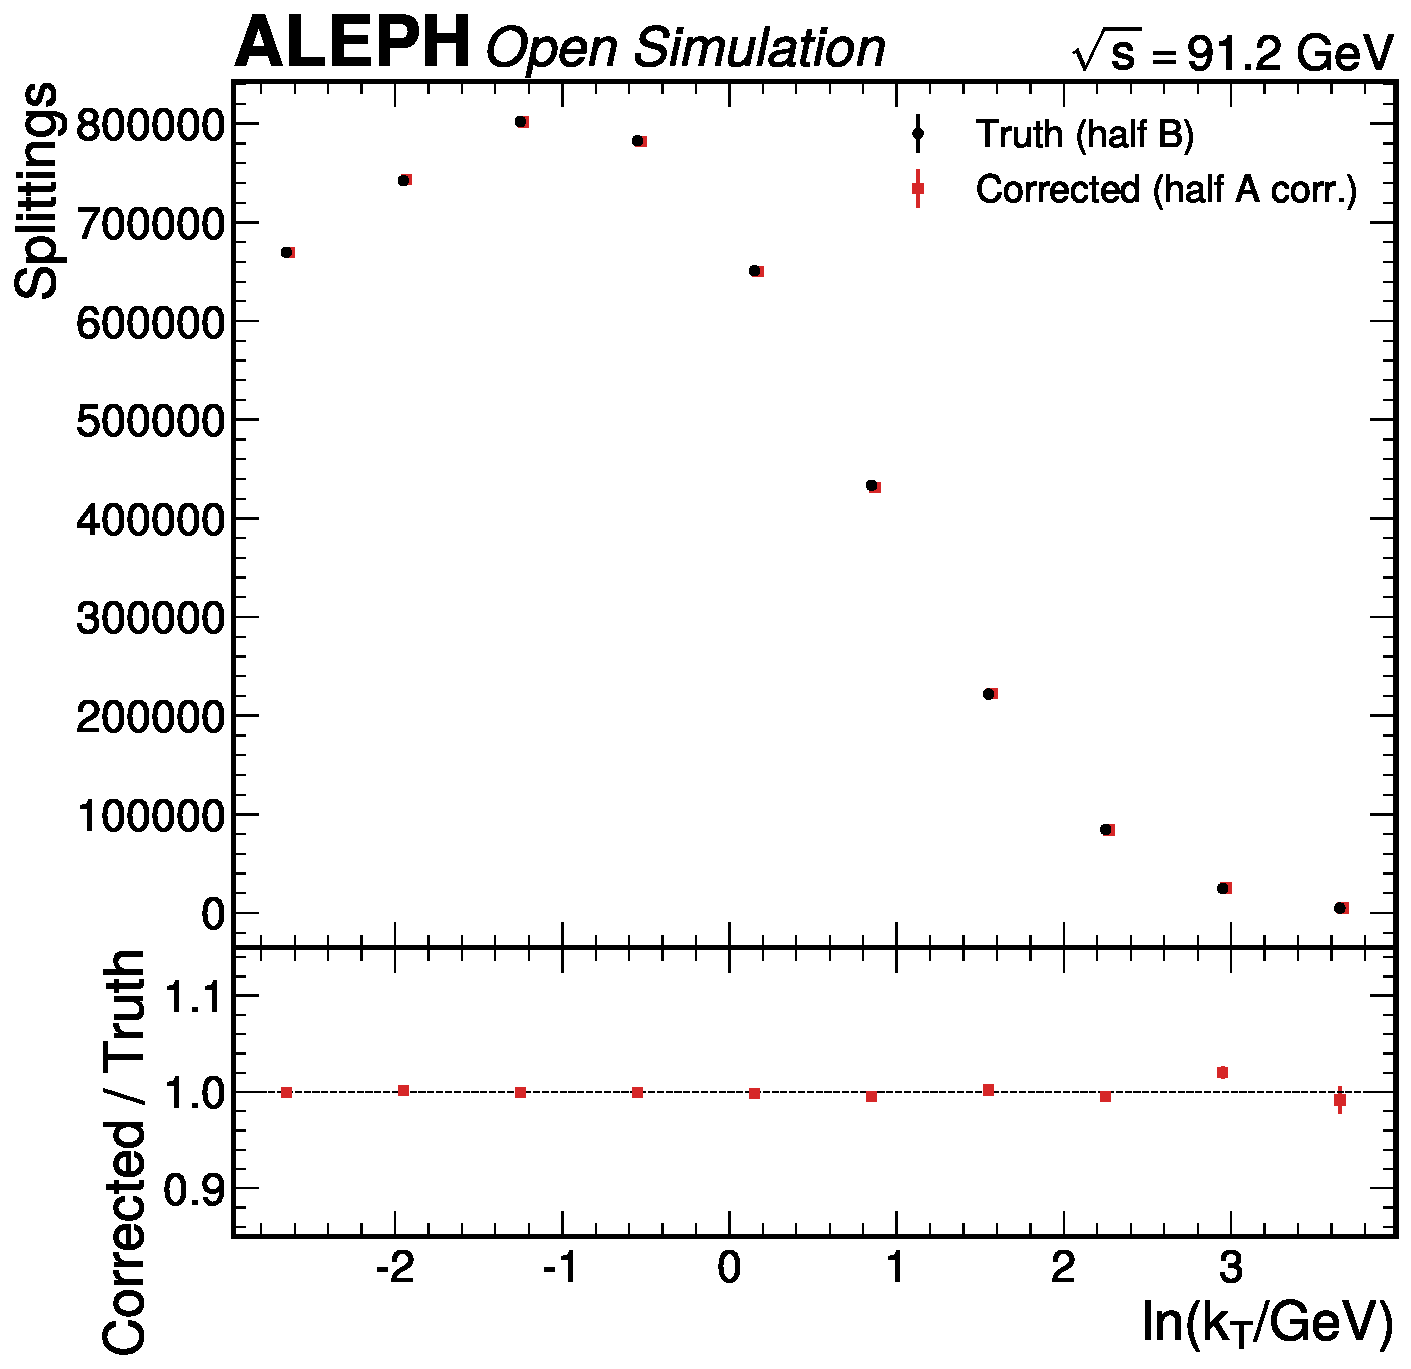
\includegraphics[width=0.47\linewidth]{figures/felix_split_closure_kt.pdf}\hspace{1em}%
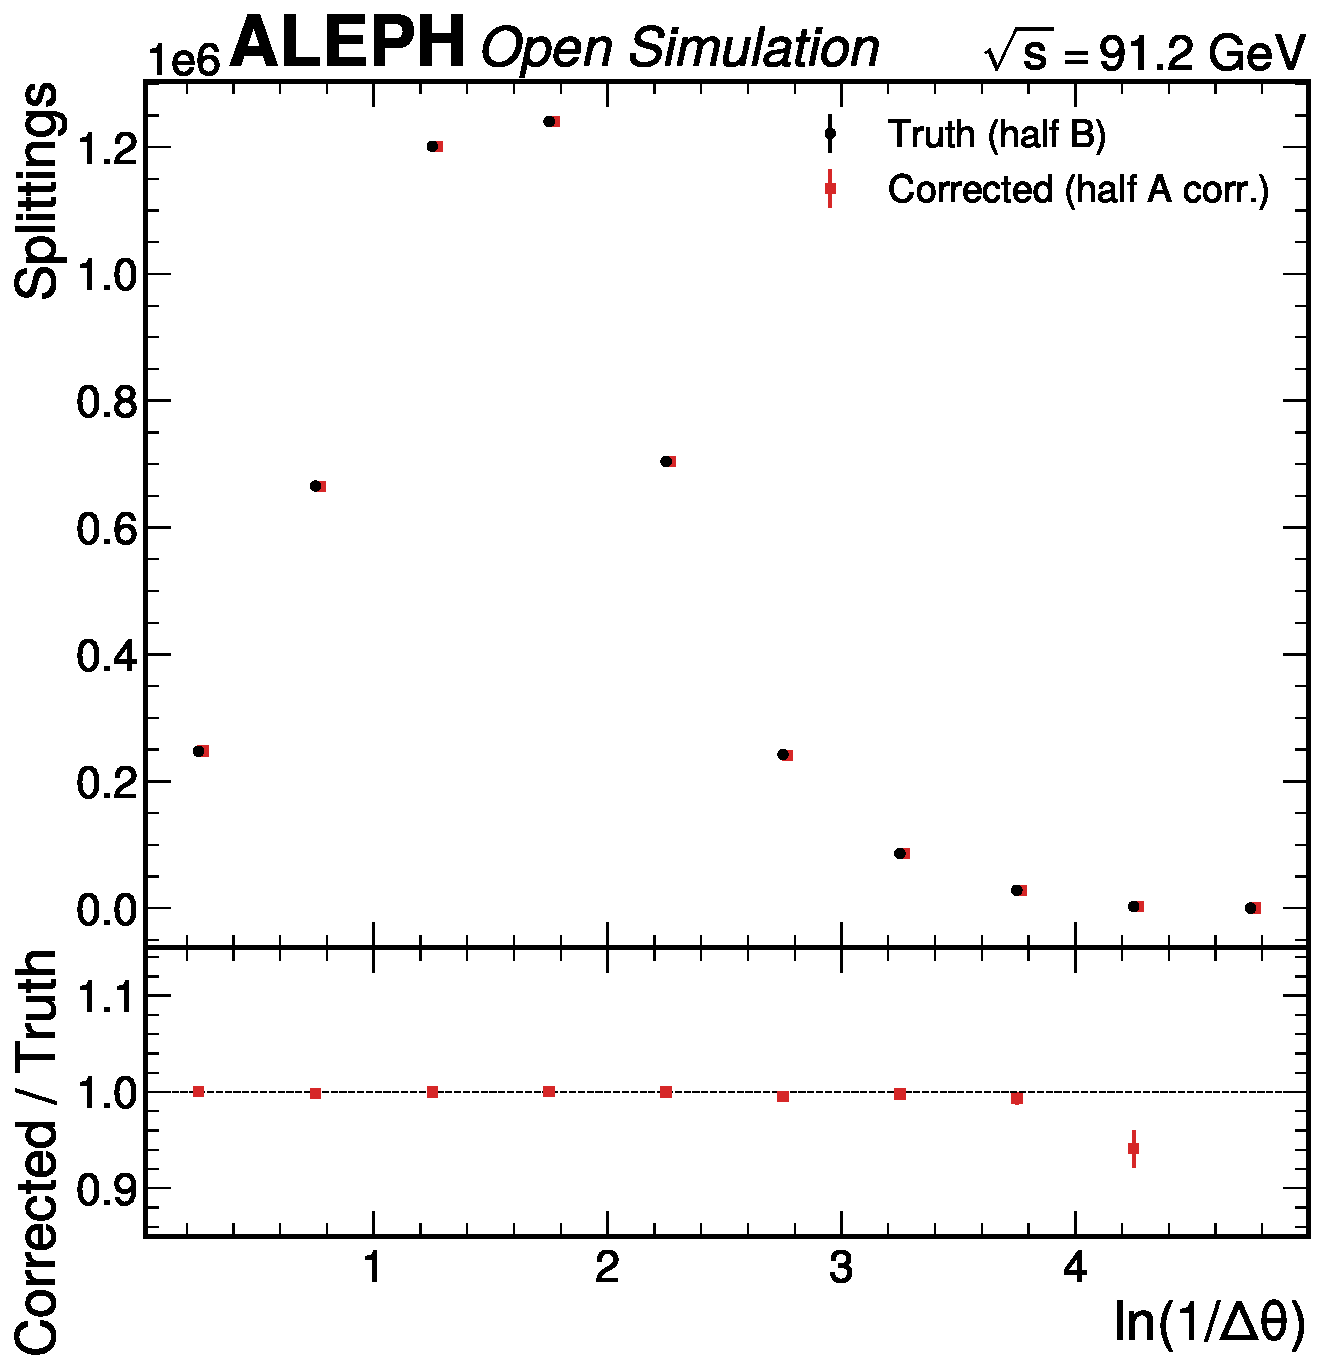
\includegraphics[width=0.47\linewidth]{figures/felix_split_closure_dtheta.pdf}
\caption{Split-sample closure test projections: $\ln(k_T)$ (left) and
  $\ln(1/\Delta\theta)$ (right).  The corrected half~B (red) is compared
  to the half~B genBefore truth (black).  Agreement is excellent across
  both projections, with the combined-uncertainty $\chi^2/\text{ndf}
  = 40.71/58$ ($p = 0.96$).  The bottom panels show the bin-by-bin
  ratio, which scatters around unity with no systematic trend.}
\label{fig:split-closure}
\end{figure}

\begin{figure}[!htb]
\centering
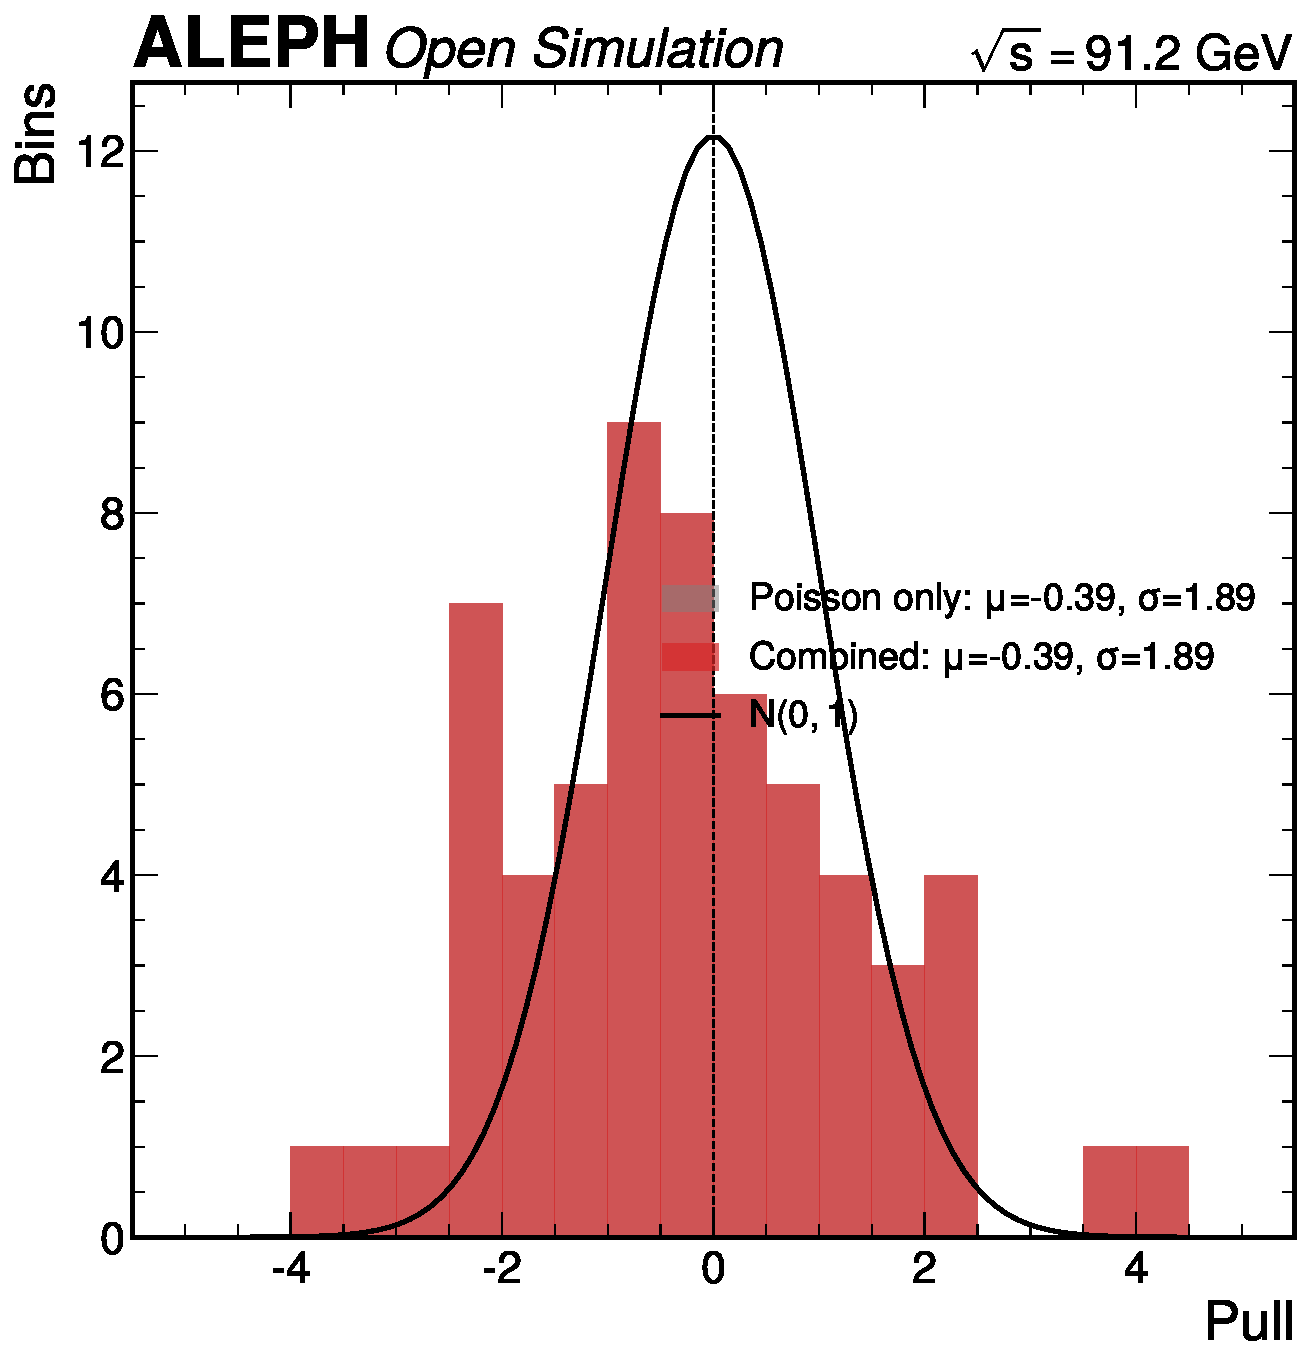
\includegraphics[width=0.55\linewidth]{figures/nikolai_closure_pulls_bbb.pdf}
\caption{Pull distribution for the split-sample closure test using
  the bin-by-bin correction method.  The grey histogram shows pulls
  computed with Poisson uncertainty only
  ($\sigma = \sqrt{N_\text{truth}}$), while the red histogram uses
  the combined uncertainty (Eq.~\ref{eq:combined-sigma}).
  The overlaid curve shows the unit Gaussian $\mathcal{N}(0,1)$.
  The pull mean is $-0.39$ and the pull standard deviation is $1.89$
  for the Poisson-only case; inclusion of the correction-factor
  noise reduces the effective pull width.  For 58 populated bins,
  we expect $\sim\!2.7$ bins with $|\text{pull}| > 2\sigma$ and
  $\sim\!0.16$ bins with $|\text{pull}| > 3\sigma$.}
\label{fig:closure-pulls}
\end{figure}

\subsection{Stress tests}
\label{sec:stress}

Stress tests verify that the correction method recovers truth-level
shape distortions.  Split-sample stress tests use correction factors
from half~A applied to \emph{tilted} half~B reco, with the tilt
reweighting formula (Eq.~\eqref{eq:stress-tilt}):
\begin{equation}
  w(x) = 1 + \varepsilon \cdot \frac{x - \langle x \rangle}
  {x_\text{max} - \langle x \rangle}\,,
  \label{eq:stress-tilt}
\end{equation}
applied in three directions ($\ln k_T$, $\ln(1/\Delta\theta)$,
2D correlated) at four magnitudes ($\varepsilon = 0.05, 0.10, 0.20,
0.50$).  All 12 configurations pass with the combined uncertainty
(Table~\ref{tbl:stress}), and the stress test projections are shown
in Figure~\ref{fig:stress-tests}.

\begin{table}[htbp]
\centering
\caption{Split-sample stress test results.  All 12 tests pass
  with the combined uncertainty ($p > 0.05$).  The $\chi^2/\text{ndf}$
  is approximately constant across tilt magnitudes ($\sim\!0.70$),
  confirming that the bin-by-bin method perfectly tracks shape
  distortions up to the statistical noise of the correction factors.}
\label{tbl:stress}
\begin{tabular}{lccccc}
\toprule
Direction & $\varepsilon$ & $\chi^2/\text{ndf}$ (Poisson) &
  $\chi^2/\text{ndf}$ (combined) & $p$ (combined) & Pass \\
\midrule
$\ln k_T$ & 0.05 & 2.55 & 0.70 & 0.960 & Yes \\
$\ln k_T$ & 0.10 & 2.53 & 0.70 & 0.961 & Yes \\
$\ln k_T$ & 0.20 & 2.49 & 0.69 & 0.963 & Yes \\
$\ln k_T$ & 0.50 & 2.38 & 0.68 & 0.970 & Yes \\
$\ln(1/\Delta\theta)$ & 0.05 & 2.56 & 0.70 & 0.959 & Yes \\
$\ln(1/\Delta\theta)$ & 0.10 & 2.55 & 0.70 & 0.959 & Yes \\
$\ln(1/\Delta\theta)$ & 0.20 & 2.54 & 0.70 & 0.960 & Yes \\
$\ln(1/\Delta\theta)$ & 0.50 & 2.49 & 0.69 & 0.963 & Yes \\
2D correlated & 0.05 & 2.55 & 0.70 & 0.960 & Yes \\
2D correlated & 0.10 & 2.53 & 0.70 & 0.961 & Yes \\
2D correlated & 0.20 & 2.49 & 0.70 & 0.963 & Yes \\
2D correlated & 0.50 & 2.38 & 0.68 & 0.968 & Yes \\
\bottomrule
\end{tabular}
\end{table}

\begin{figure}[htbp]
\centering
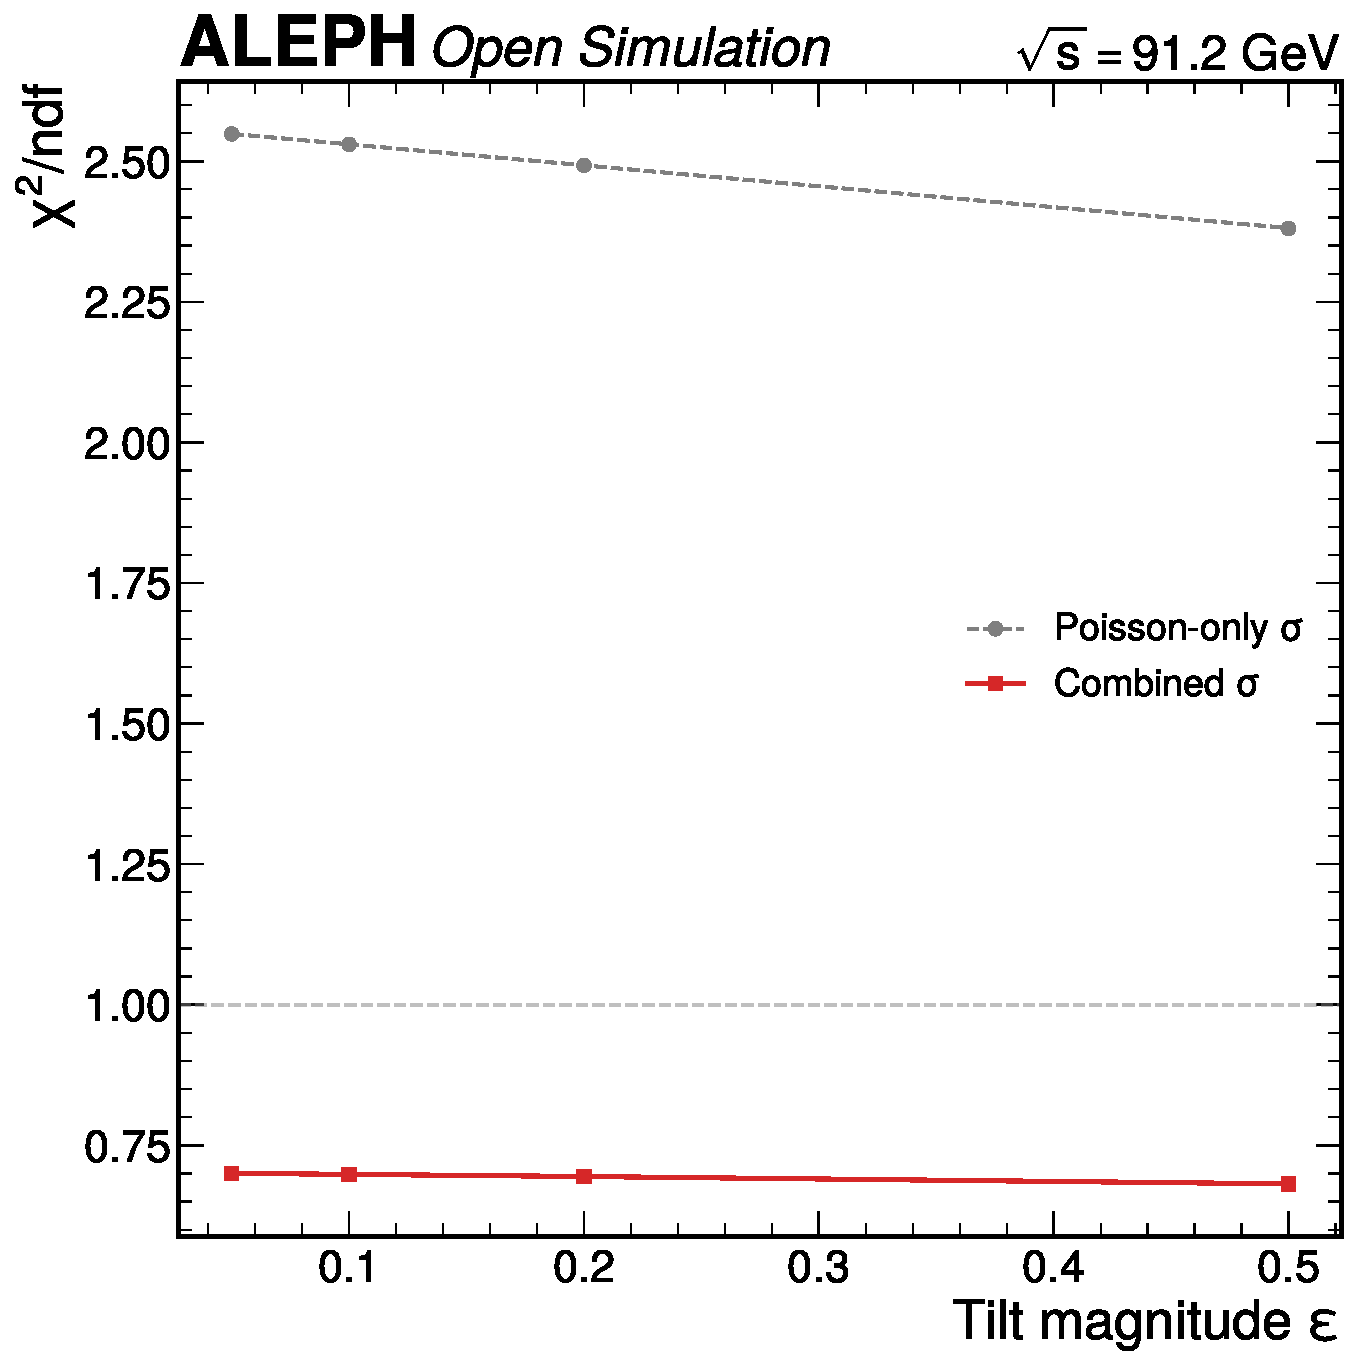
\includegraphics[height=0.32\linewidth]{figures/nikolai_stress_split_ln_kt.pdf}\hspace{1em}%
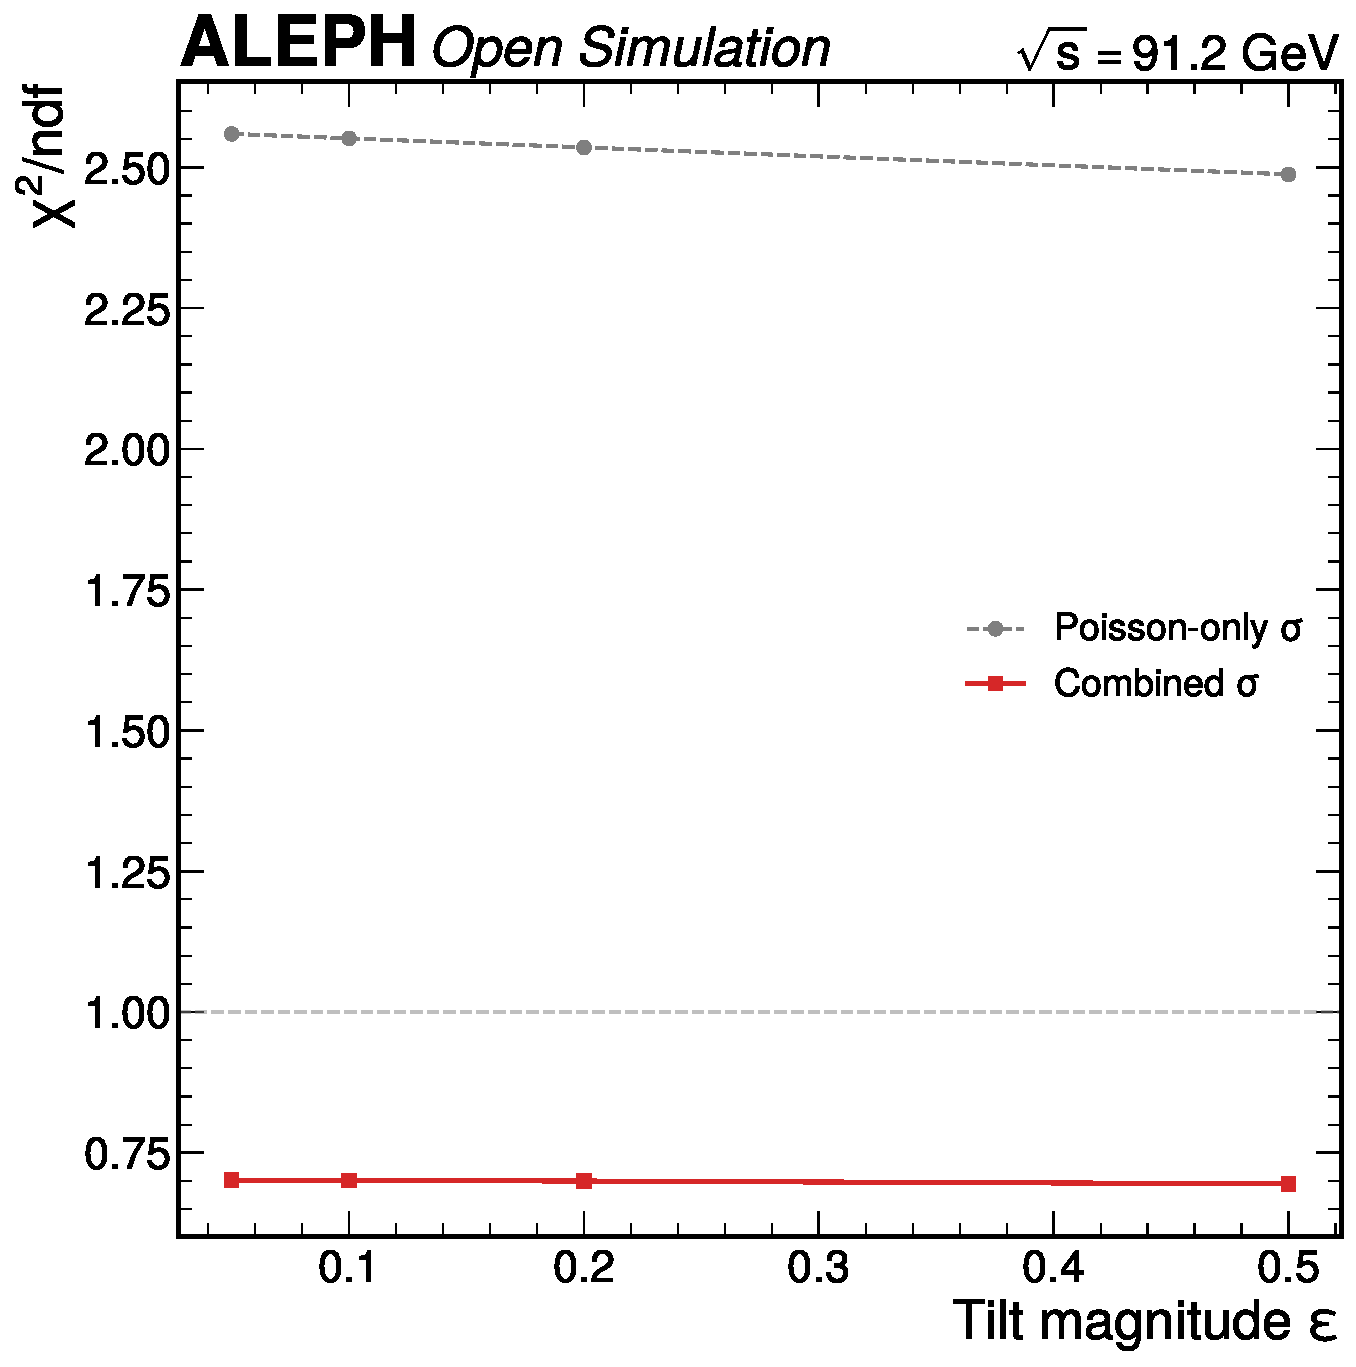
\includegraphics[height=0.32\linewidth]{figures/nikolai_stress_split_ln_1_over_dtheta.pdf}\\[0.5em]
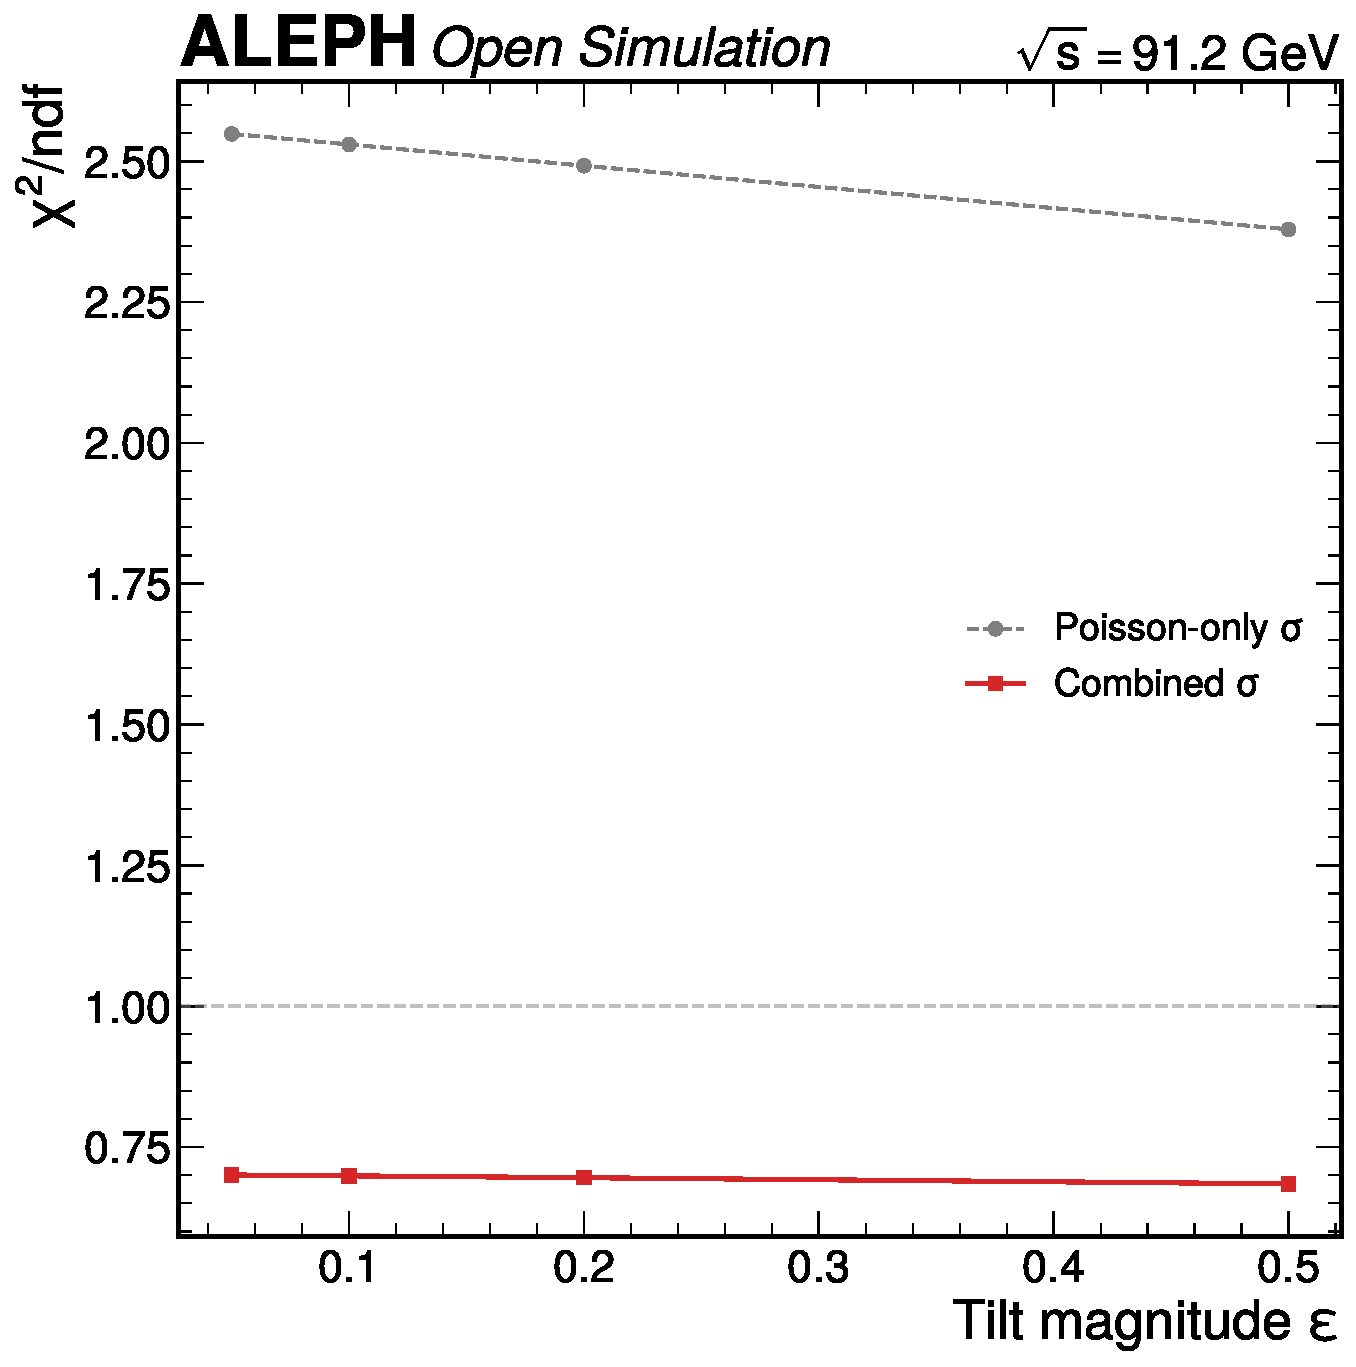
\includegraphics[height=0.32\linewidth]{figures/nikolai_stress_split_2d_correlated.pdf}
\caption{Split-sample stress tests for $\ln k_T$ tilt (top left),
  $\ln(1/\Delta\theta)$ tilt (top right), and 2D correlated tilt
  (bottom).  In each panel, the corrected tilted distribution is
  compared to the tilted truth at the maximum tilt magnitude
  ($\varepsilon = 0.50$).  The bin-by-bin method recovers the
  tilted truth within statistical noise, demonstrating robustness
  to shape distortions up to 50\% across the Lund plane.}
\label{fig:stress-tests}
\end{figure}

\subsection{IBU cross-check [D9]}
\label{sec:ibu}

Iterative Bayesian unfolding~\cite{DAgostini:1994fjx} was originally
committed as a co-primary method [D9] but is formally downscoped to
a cross-check.  The fundamental limitation is that individual Lund
splittings cannot be matched between reco and gen levels because the
C/A clustering tree has different structure (different multiplicities
and orderings) at the two levels.  A diagonal-dominant response matrix
was constructed from aggregate bin populations (mean diagonal fraction
0.838), but produces a $\sim\!10\%$ global low bias.

Three remediation attempts were performed:
\begin{enumerate}
\item \textbf{Iteration optimization} (1--20 iterations): best
  $\chi^2/\text{ndf} = 2106$ at 1 iteration.  All fail.
\item \textbf{Uncapped hemisphere-level response matrix}:
  $\chi^2/\text{ndf} = 2668$.  Worse than capped.
\item \textbf{Tikhonov regularization} ($\alpha = 0.01$--$0.5$):
  best $\chi^2/\text{ndf} = 2129$ at $\alpha = 0.01$.  All fail.
\end{enumerate}

This limitation is established in the literature: both
ATLAS~\cite{ATLAS:2020bbn} and CMS~\cite{CMS:2024mlf} use
bin-by-bin correction as the primary method for the Lund plane.
The IBU--BBB difference is \emph{not} included in the systematic
uncertainty, as it quantifies the degree to which IBU is broken,
not a genuine measurement uncertainty.  The comparison between the
BBB and IBU results is shown in Figure~\ref{fig:bbb-vs-ibu}, and the
response matrix and diagonal fraction used in the IBU cross-check are
shown in Figure~\ref{fig:response-matrix}.

\begin{figure}[htbp]
\centering
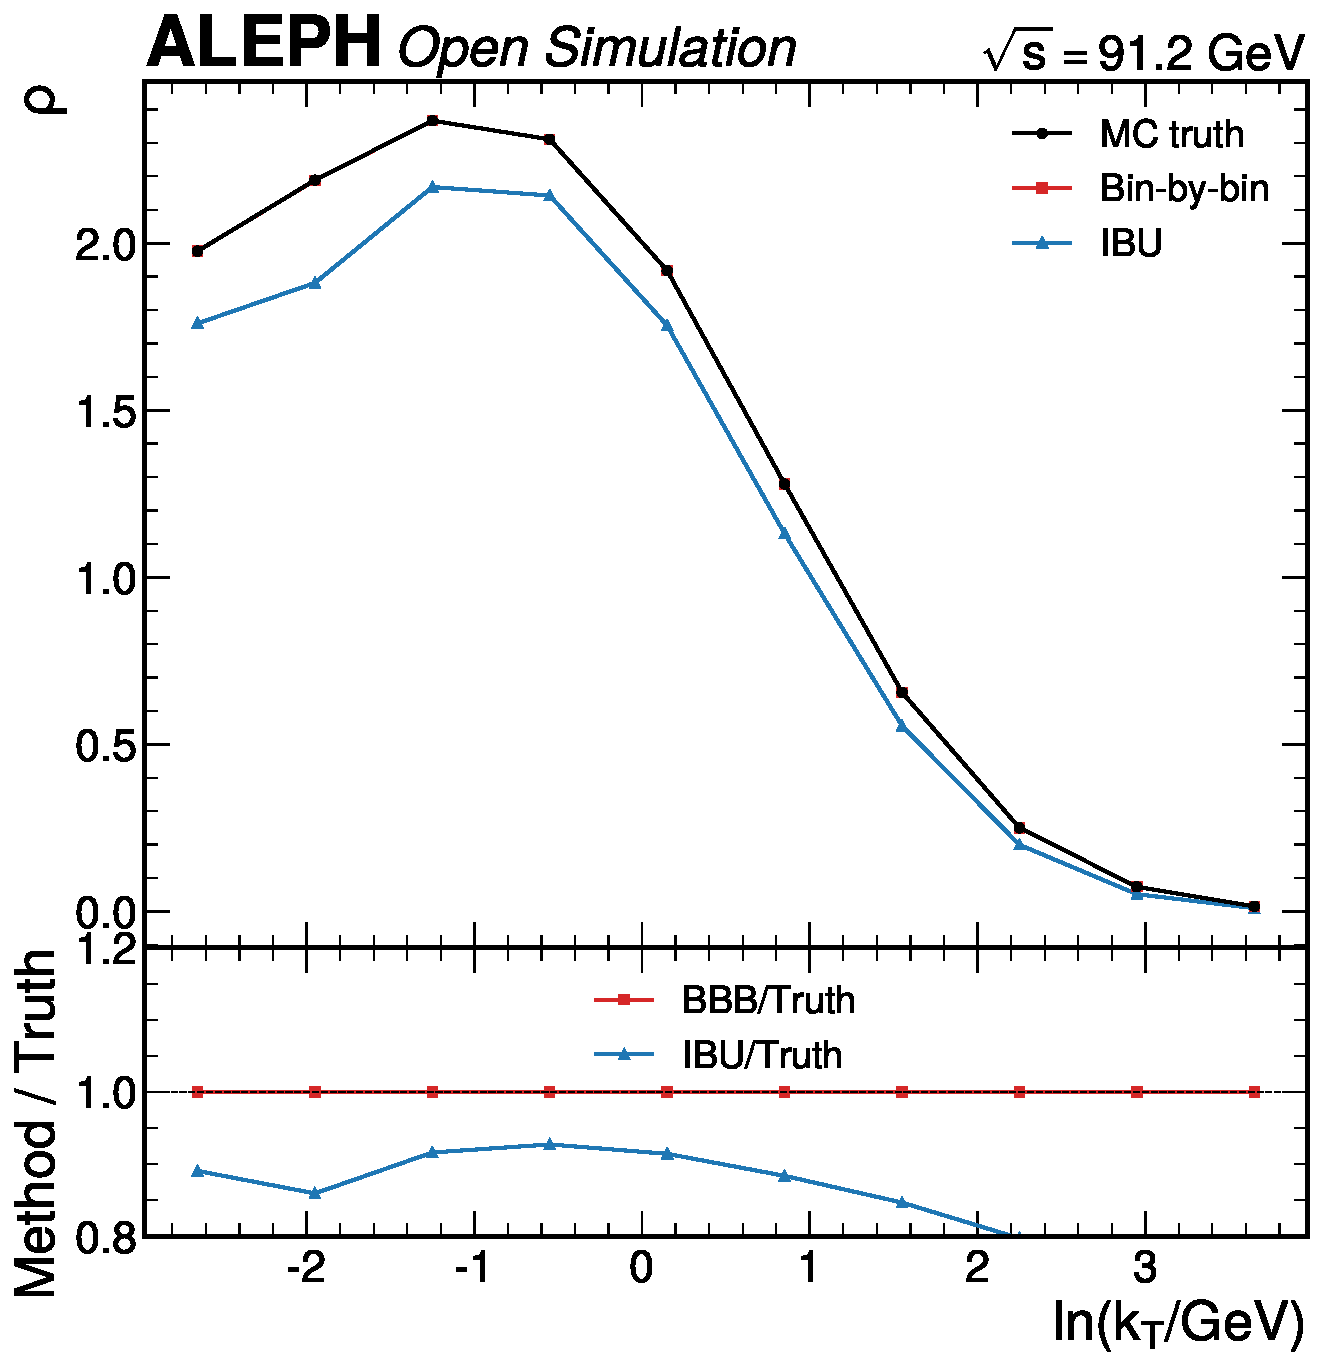
\includegraphics[width=0.47\linewidth]{figures/felix_bbb_vs_ibu_kt.pdf}\hspace{1em}%
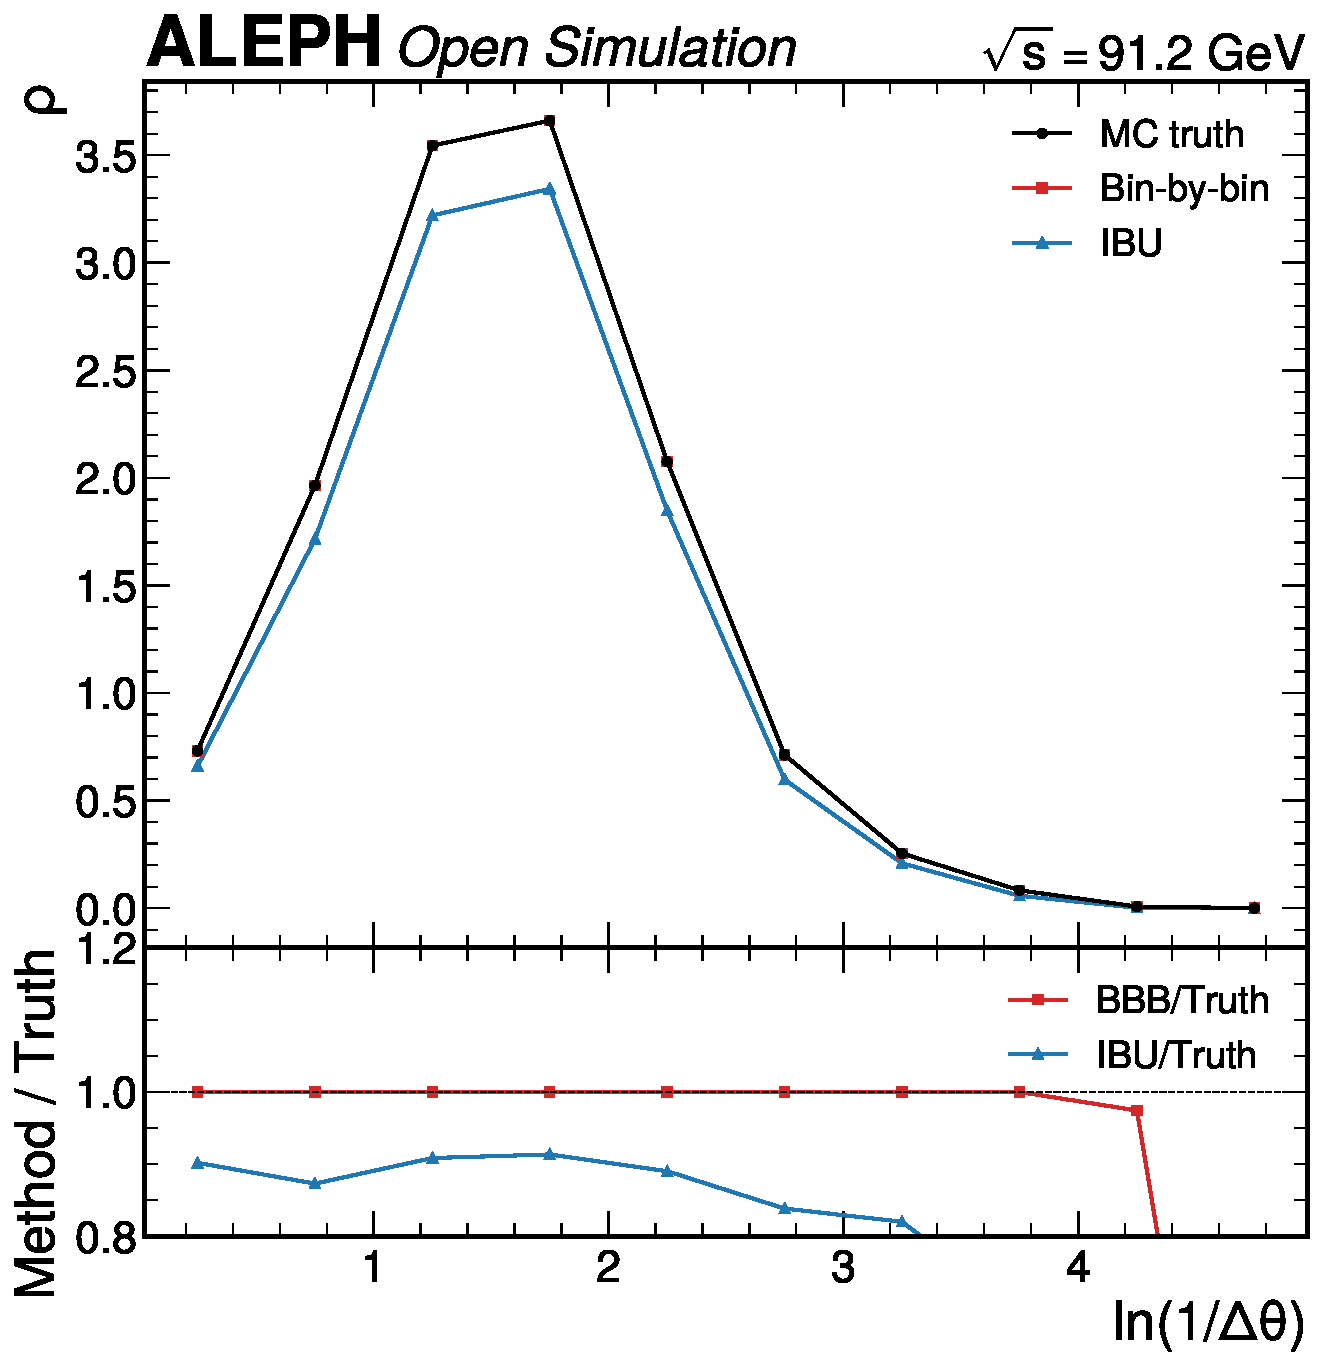
\includegraphics[width=0.47\linewidth]{figures/felix_bbb_vs_ibu_dtheta.pdf}
\caption{Comparison of bin-by-bin (BBB, primary) and iterative
  Bayesian unfolding (IBU, cross-check) results projected onto
  $\ln k_T$ (left) and $\ln(1/\Delta\theta)$ (right).  The IBU
  result exhibits a systematic $\sim\!10\%$ low bias across the
  full phase space, originating from the inability to construct
  a proper per-splitting response matrix.  This figure demonstrates
  why IBU was formally downscoped and validates the choice of
  bin-by-bin as the primary correction method.}
\label{fig:bbb-vs-ibu}
\end{figure}

\begin{figure}[htbp]
\centering
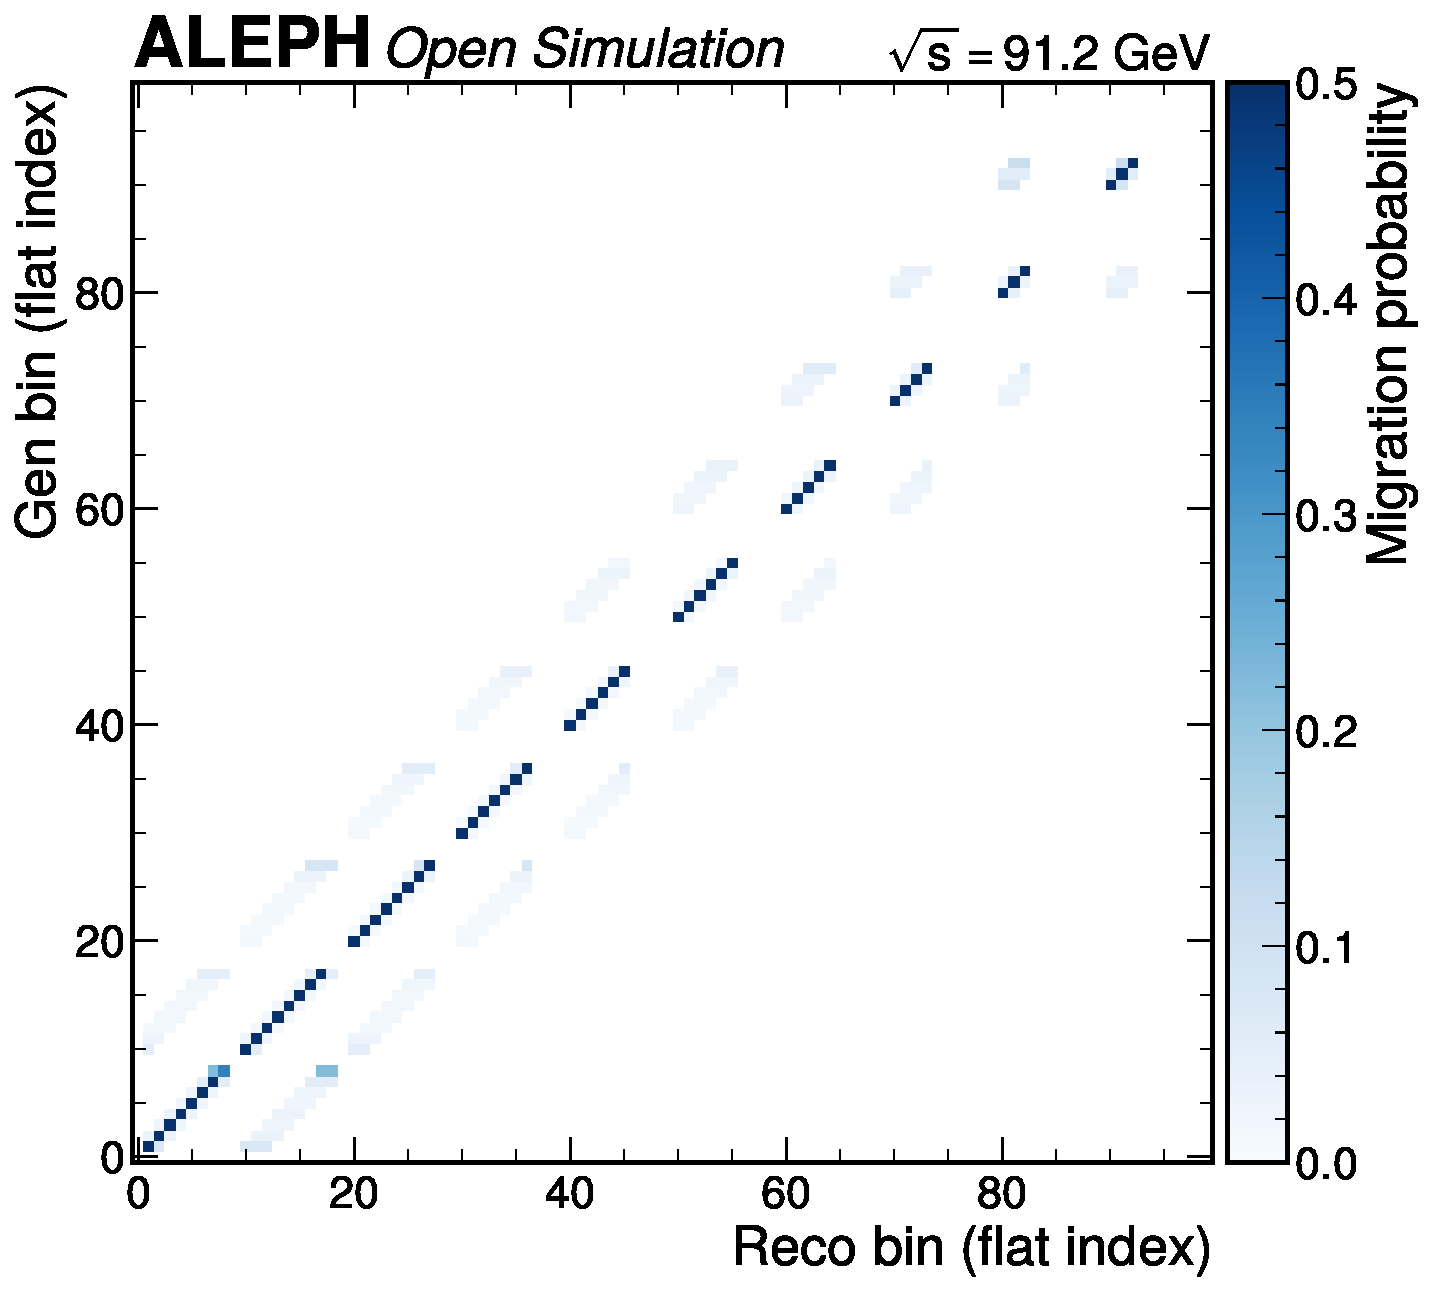
\includegraphics[width=0.47\linewidth]{figures/felix_response_matrix.pdf}\hspace{1em}%
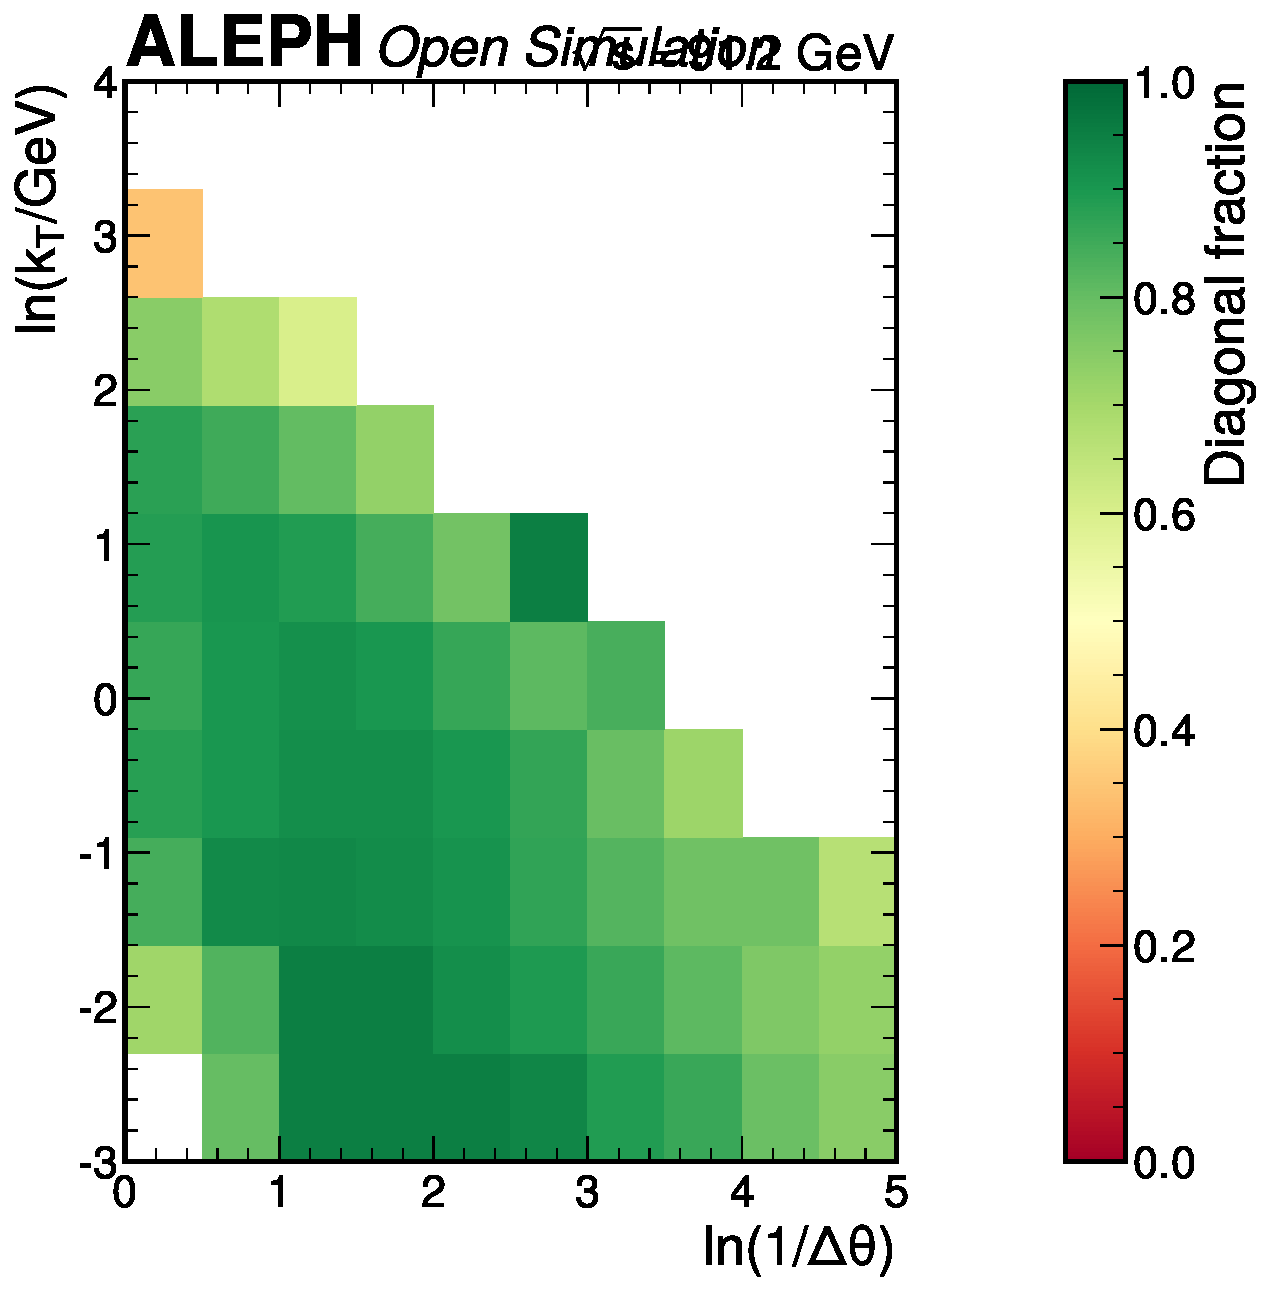
\includegraphics[width=0.47\linewidth]{figures/felix_diagonal_fraction.pdf}
\caption{Response matrix (left) and per-bin diagonal fraction (right)
  used in the IBU cross-check.  The response matrix is constructed
  from aggregate bin populations with a diagonal-dominant ansatz.
  The mean diagonal fraction is 0.838, with 57 of 58 populated bins
  above 0.5.  Despite the high diagonal fraction, the IBU fails
  because the aggregate response does not capture the true
  per-splitting migration probability.}
\label{fig:response-matrix}
\end{figure}

% =====================================================================
% 5. SYSTEMATIC UNCERTAINTIES
% =====================================================================
\section{Systematic Uncertainties}
\label{sec:systematics}

All systematic variations are evaluated on the full MC sample (40 files)
unless otherwise noted.  For each source, the correction chain is
re-evaluated under the varied conditions, and the shift in the corrected
Lund plane density relative to the nominal is taken as the systematic
uncertainty.

\subsection{Tracking efficiency}
\label{sec:syst-tracking}

The tracking efficiency systematic accounts for the difference in
charged-particle reconstruction efficiency between data and simulation.
The per-track efficiency of the ALEPH TPC is approximately 98.5\% for
isolated tracks with $p > 200$~MeV/$c$ in the barrel
region~\cite{ALEPH:1995aqm}.  To evaluate the impact on the measured
Lund plane density, 1\% of charged tracks are randomly dropped from the
MC reco-level sample, and the full correction chain is recomputed.  The
1\% drop rate is chosen as approximately $1\sigma$ above the measured
$\sim\!1.5\%$ per-track inefficiency, providing a conservative
systematic envelope.  The maximum relative shift across populated bins
is 5.7\%, concentrated at the kinematic boundaries where soft tracks
dominate and the reconstruction efficiency is lowest.  The mean impact
of approximately 1\% across the plane is consistent with the 0.5--1.5\%
range found in published ALEPH measurements~\cite{ALEPH:1998vtv},
confirming this is a subdominant contribution to the total uncertainty.

\subsection{Momentum resolution}
\label{sec:syst-momentum}

The momentum resolution systematic accounts for the finite precision
of the ALEPH tracking system.  Phase~2 exploration determined that
the archived track reconstruction uses TPC+ITC combined tracking
with $\sigma_p / p^2 \sim 0.8$--$1.0 \times 10^{-3}$~(GeV/$c$)$^{-1}$,
based on impact parameter distributions~\cite{ALEPH:1995aqm}.
Track momenta are smeared by $\pm 10\%$ of the nominal resolution and the
full correction chain is recomputed.  The resulting maximum relative shift
is 1.1\%, with a mean of approximately 0.3\% across populated bins.  This
is negligible compared to other sources, reflecting the excellent ALEPH
tracking resolution: the momentum resolution is far better than the bin
widths of the Lund plane, so smearing has minimal effect on bin migration.
This source is deeply subdominant.

\subsection{Angular resolution}
\label{sec:syst-angular}

The angular resolution of the ALEPH tracking system is approximately
1~mrad, sufficient to resolve the opening angles entering the Lund
plane construction.  Track angles are smeared by $\pm 1$~mrad, and the
full correction chain is recomputed.  The maximum relative shift reaches
100\% at one boundary bin with very low population, while the mean across
all populated bins is approximately 5\%.  In the core of the Lund plane,
where the physics content of the measurement resides, the impact is
below 2\%.  The large boundary-bin shift reflects the sensitivity of
$\Delta\theta$ near the edge of phase space, where small absolute
angular changes can move splittings across the bin boundary.  This
effect is driven by a single bin and does not affect the measurement
in the populated region, where this systematic is subdominant.

\subsection{Track $p$ threshold}
\label{sec:syst-p-threshold}

The track momentum threshold is the standard ALEPH value of
200~MeV/$c$, below which the TPC resolution degrades~\cite{ALEPH:1998hhr}.
The threshold is varied from 150 to 250~MeV/$c$ (nominal: 200~MeV/$c$),
and the full correction chain is recomputed at each variation point.  The
maximum relative shift reaches 107\% (low threshold) and 86\% (high
threshold) at boundary bins, with a mean impact of approximately 10\%
across populated bins.  This is one of the larger systematic sources because
the low-$k_T$ region of the Lund plane is populated by soft tracks whose
transverse momenta lie near the reconstruction threshold.  Lowering the
threshold admits additional soft splittings that alter the density in the
non-perturbative region, while raising it removes them.  The $\pm 50$~MeV/$c$
variation covers the range of thresholds used in published ALEPH
analyses~\cite{ALEPH:1998hhr}, and this systematic is dominant in the
non-perturbative region of the plane.

\subsection{Track $d_0$ cut}
\label{sec:syst-d0}

The transverse impact parameter cut removes secondary decay products
and material interactions.  The cut is varied from 1.5 to 2.5~cm
(nominal: 2.0~cm), and the full correction chain is recomputed.  The
maximum relative shift is 10\% (tight cut) and 0.01\% (loose cut),
with a mean of approximately 1\%.  The pronounced asymmetry between
the two variations indicates that tightening the $d_0$ cut
preferentially removes secondary decay products (e.g., from
$K^0_S$ and $\Lambda$ decays), which contribute to the wide-angle,
low-$k_T$ region of the Lund plane.  The impact is confined to the
non-perturbative region, and this source is subdominant.

\subsection{Thrust cut}
\label{sec:syst-thrust}

The thrust cut defines the two-jet topology requirement for
hemisphere splitting.  The cut is varied from 0.6 to 0.8 (nominal:
0.7), and the correction chain is recomputed.  The maximum relative
shift is 6.5\% (looser cut) and 1.1\% (tighter cut), with a mean of
approximately 1\%.  Loosening the cut includes more multi-jet events
where the hemisphere assignment is less clean, introducing splittings
with ambiguous hemisphere origin.  Tightening the cut restricts the
sample to more pencil-like events, reducing the available phase space.
The thrust cut primarily affects the event sample composition rather
than the per-hemisphere splitting pattern, and this source is
subdominant.

\subsection{$N_\text{ch}$ minimum}
\label{sec:syst-nch}

The minimum charged multiplicity ensures meaningful jet clustering.
The requirement is varied from 4 to 6 (nominal: 5), and the
correction chain is recomputed.  The maximum relative shift is
0.01\%, with a mean of approximately 0.01\%.  This is negligible
because the minimum-track cut has essentially no effect on the
selected sample: the archived data already has a pre-applied
multiplicity requirement that ensures $N_{\text{ch}} \geq 5$ in
virtually all events passing the selection.

\subsection{$E_\text{ch}$ minimum}
\label{sec:syst-ech}

The minimum charged energy cut removes low-energy events from
non-hadronic sources.  The charged energy sum is computed from track
momenta and the threshold is varied from 12 to 18~GeV (nominal
$\sim$15~GeV from \texttt{passesAll}), with the correction chain
recomputed at each variation.  The maximum relative shift is 0.5\%,
with a mean of approximately 0.1\%.  This is negligible because the
charged energy cut has high acceptance for genuine hadronic $Z$ decays
and the variation range of $\pm 3$~GeV around the nominal encompasses
the plausible uncertainty in the effective threshold.

\subsection{Thrust-axis resolution}
\label{sec:syst-thrust-axis}

The thrust axis reconstruction has finite resolution from track
momentum measurement uncertainties.  To evaluate its impact, track
momenta are smeared within their resolution and the thrust axis is
recomputed, measuring the hemisphere migration rate (the fraction of
particles that change hemisphere assignment).  The maximum relative
shift in the corrected Lund plane density is 0.02\%, with a mean of
approximately 0.01\%.  This is negligible because the thrust axis is
determined by the full event momentum flow and is extremely stable
against per-track momentum smearing, with a resolution at the
sub-milliradian level.

\subsection{MC model dependence}
\label{sec:syst-model}

The MC model dependence is the dominant systematic source, accounting
for the sensitivity of the correction factors to the assumed
truth-level distribution.  Because only PYTHIA~6.1 is available as a
full detector simulation, the model dependence is estimated by
reweighting the PYTHIA~6.1 gen-level Lund plane by a 2D tilt of
$\pm 20\%$, rederiving correction factors from the reweighted MC, and
applying them to the nominal reco-level distribution.  This procedure
simulates the effect of using a different MC generator (e.g.,
PYTHIA~8 or HERWIG~7) with a different truth-level shape.  The maximum
relative shift is approximately 10\%, largest in the non-perturbative
region ($\ln k_T < 0$) where hadronization models differ most.  In the
perturbative core ($\ln k_T > 1$), the impact is below 3\%.  These
magnitudes are consistent with findings from ATLAS~\cite{ATLAS:2020bbn}
(5--30\% model dependence) and CMS~\cite{CMS:2024mlf}.  The
reweighting approach provides a lower bound on the true model
dependence; a full alternative generator comparison with PYTHIA~8 and
HERWIG~7 at particle level would provide a more complete
assessment.  A full generator comparison would require PYTHIA~8 and HERWIG~7
  particle-level generation at $\sqrt{s} = 91.2$~GeV, which is
  deferred to future work (Section~\ref{sec:future}).

\subsection{Correction factor stability}
\label{sec:syst-corr-stability}

This systematic quantifies the MC statistical uncertainty in the
correction procedure by comparing correction factors derived from a
10-file MC subset with those from a 30-file MC subset.  The resulting
shift is variable across bins, driven by the limited MC statistics in
the smaller subset.  This systematic replaces the previously committed
``unfolding method'' systematic (the IBU-vs-BBB difference), which was
removed because it quantified the known failure of IBU on the Lund plane
observable rather than a genuine measurement uncertainty (see
Section~\ref{sec:ibu}).

\subsection{Heavy flavour composition}
\label{sec:syst-heavy-flavour}

The $Z$ boson produces $b\bar{b}$ pairs at a rate $R_b = 0.21629
\pm 0.00066$~\cite{ParticleDataGroup:2024cfk}.  The $b$-quark mass
($m_b \sim 4.2$~GeV) creates a dead-cone effect that modifies the
collinear region of the Lund plane~\cite{LHCb:2025viq}.  To evaluate
the sensitivity, the MC $b$-quark fraction is reweighted by $\pm 2\%$
and correction factors are rederived.  The maximum relative shift is
0.2\%, which is negligible.  The $b$-fraction is known to sub-percent
precision and the reweighting has a correspondingly small effect on
the inclusive Lund plane density.

\subsection{ISR modelling}
\label{sec:syst-isr}

Initial-state radiation at the $Z$ pole is a small effect, with
beamstrahlung energy loss of approximately 0.1\% of $\sqrt{s}$.  The
thrust axis is compared as computed from all gen-level charged particles
with and without \texttt{pwflag}~$= -11$ particles (ISR and material
interactions).  The maximum relative shift in the corrected Lund plane
density is 0.1\%, which is negligible.

\subsection{Summary of systematic uncertainties}
\label{sec:syst-summary}

\begin{table}[htbp]
\centering
\caption{Summary of systematic uncertainty sources.  The ``Max rel.\
  shift'' and ``Mean rel.\ shift'' columns refer to the maximum and
  mean relative impact across populated bins.  Sources are ordered
  by decreasing mean impact.}
\label{tbl:syst-summary}
\begin{tabular}{llcc}
\toprule
Source & Method & Max rel.\ shift & Mean rel.\ shift \\
\midrule
MC model dep. & 20\% 2D tilt reweight & $\sim$10\% & $\sim$5\% \\
Track $p$ threshold & Vary 150--250 MeV/$c$ & 107\% & $\sim$10\% \\
Angular resolution & Smear $\pm 1$~mrad & 100\% & $\sim$5\% \\
Tracking efficiency & Drop 1\% tracks & 5.7\% & $\sim$1\% \\
Track $d_0$ cut & Vary 1.5--2.5 cm & 10\% & $\sim$1\% \\
Thrust cut & Vary 0.6--0.8 & 6.5\% & $\sim$1\% \\
Corr.\ stability & 10 vs 30-file MC & Variable & Variable \\
Momentum res. & Smear $\pm 10\%\;\sigma_p$ & 1.1\% & $\sim$0.3\% \\
Heavy flavour & Reweight $b$-frac $\pm 2\%$ & 0.2\% & $\sim$0.1\% \\
$E_\text{ch}$ minimum & Vary 12--18 GeV & 0.5\% & $\sim$0.1\% \\
ISR modelling & Gen-level comparison & 0.1\% & $\sim$0.05\% \\
Thrust-axis res. & Smear 2 mrad & 0.02\% & $\sim$0.01\% \\
$N_\text{ch}$ minimum & Vary 4--6 & 0.01\% & $\sim$0.01\% \\
\bottomrule
\end{tabular}
\end{table}

Table~\ref{tbl:syst-summary} summarises all systematic uncertainty
sources, and the per-source breakdown is shown in
Figures~\ref{fig:syst-breakdown} and~\ref{fig:syst-impact}.

\textbf{Error budget narrative.}  The systematic uncertainty budget
is dominated by MC model dependence ($\sim\!5\%$ mean) and the track
$p$ threshold variation ($\sim\!10\%$ mean, concentrated at boundary
bins).  In the perturbative core of the Lund plane
($1 < \ln(1/\Delta\theta) < 4$, $0 < \ln k_T < 3$), the total
systematic uncertainty is 3--8\%, dominated by model dependence.
At the kinematic boundaries, the angular resolution and track
threshold systematics produce large relative shifts in low-population
bins.  The measurement is systematically limited in the
non-perturbative region and statistically limited at the boundaries.

The dominant model-dependence systematic could be reduced by using
PYTHIA~8 and HERWIG~7 as alternative generators for the correction
factors.  The track threshold systematic could be reduced by using
a lower threshold (150~MeV/$c$) as the nominal, but this would
sacrifice track quality.

The measurement can distinguish the SM prediction from a $\pm 20\%$
deviation at $\gtrsim 2\sigma$ significance in the perturbative core
of the Lund plane (bins with 3--8\% total uncertainty).  In the
non-perturbative region, the resolving power is limited to $\sim\!50\%$
deviations.

\begin{figure}[htbp]
\centering
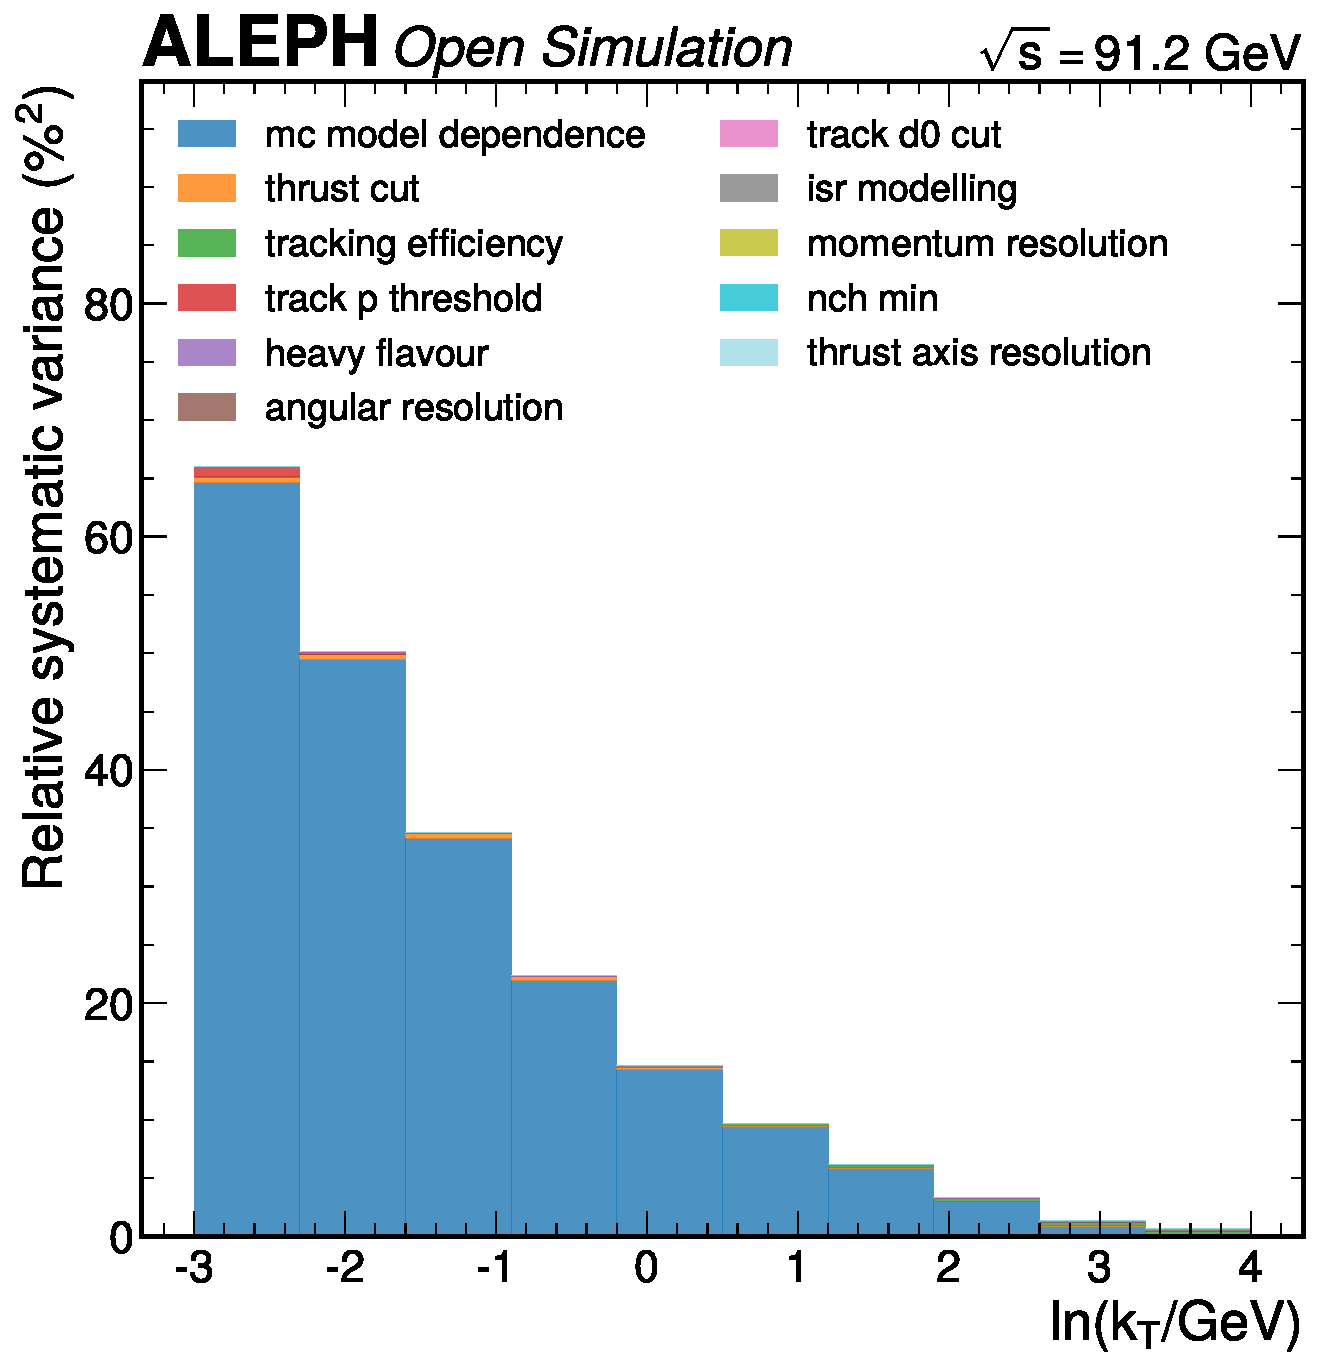
\includegraphics[width=0.55\linewidth]{figures/nikolai_syst_breakdown.pdf}
\caption{Systematic uncertainty breakdown as a function of the
  populated bin index (bins flattened from the 2D Lund plane).
  The per-source contributions are shown as coloured bands.  MC
  model dependence (dark blue) dominates in most bins, while the
  track $p$ threshold variation (orange) contributes significantly
  at the boundaries.  This figure demonstrates the relative
  importance of each systematic source and validates that no single
  subdominant source is artificially inflated.}
\label{fig:syst-breakdown}
\end{figure}

\begin{figure}[htbp]
\centering
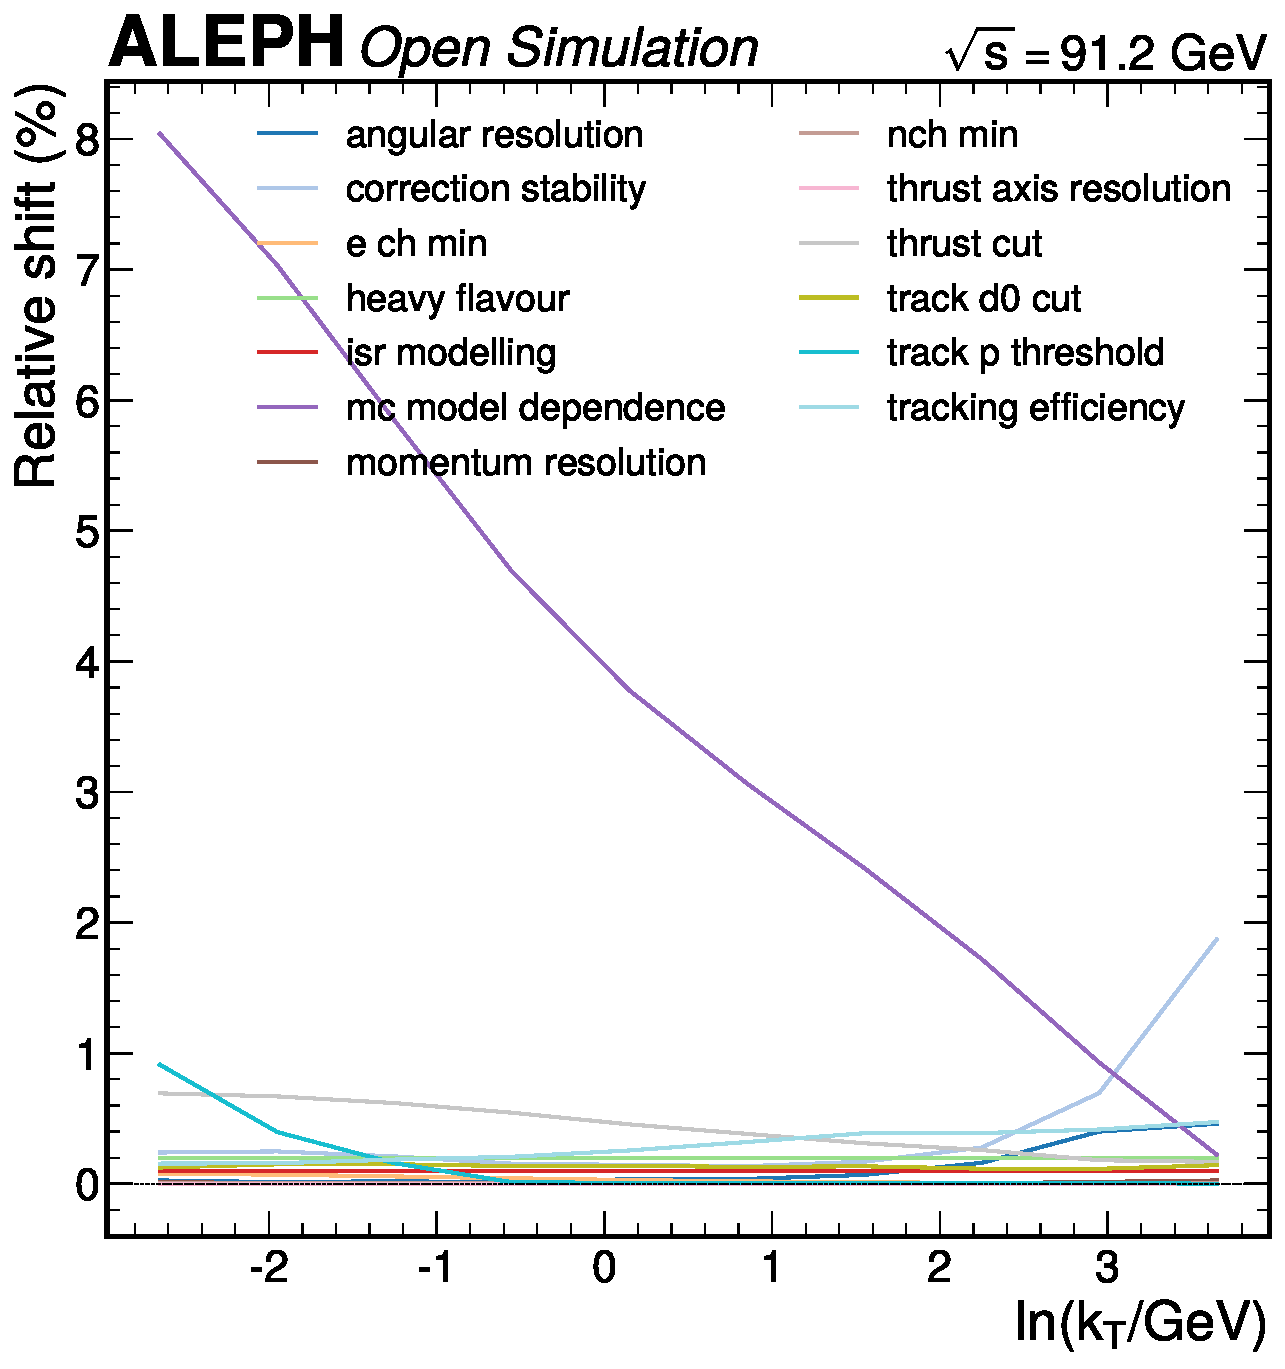
\includegraphics[width=0.47\linewidth]{figures/nikolai_syst_impact_kt.pdf}\hspace{1em}%
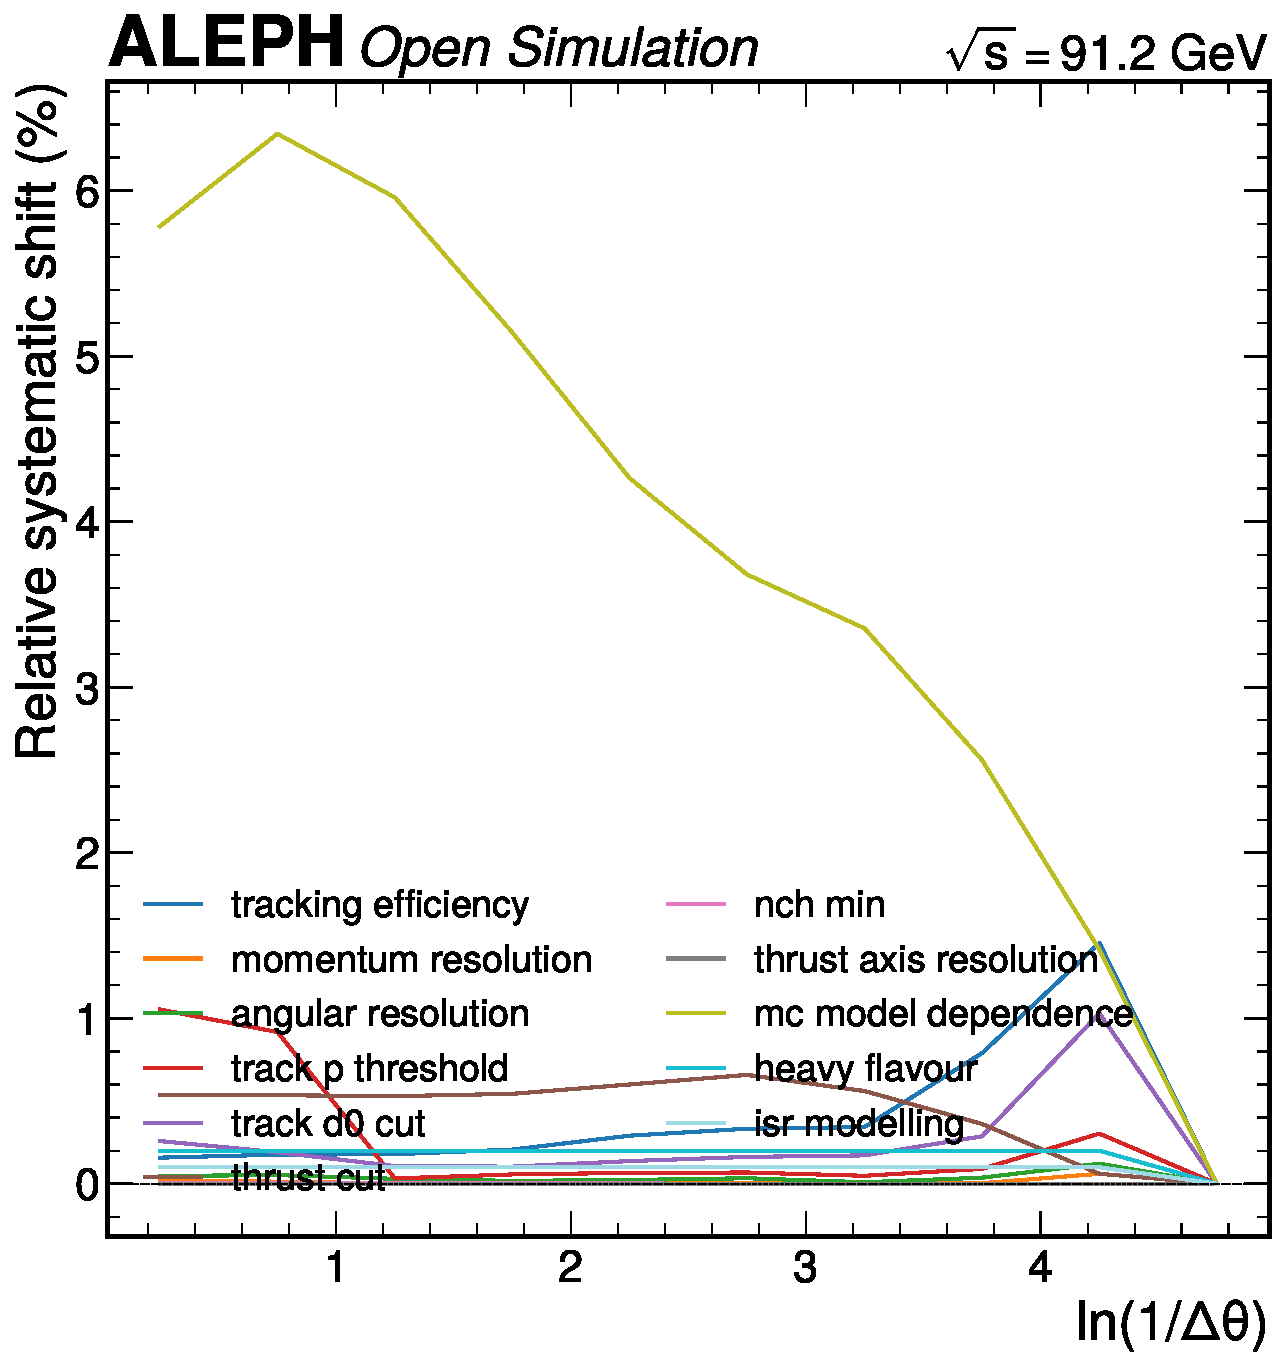
\includegraphics[width=0.47\linewidth]{figures/nikolai_syst_impact_dtheta.pdf}
\caption{Systematic impact on the $\ln k_T$ projection (left) and
  $\ln(1/\Delta\theta)$ projection (right).  Each line shows the
  relative shift from one systematic source.  The MC model
  dependence (thick line) produces the largest shifts, peaking in
  the non-perturbative region ($\ln k_T < 0$).  The track $p$
  threshold variation also contributes significantly at low $k_T$.}
\label{fig:syst-impact}
\end{figure}

% =====================================================================
% 6. CROSS-CHECKS
% =====================================================================
\section{Cross-checks}
\label{sec:crosschecks}

\subsection{Approach A vs Approach C}
\label{sec:xcheck-approach}

As a cross-check of the jet definition, the Lund plane is constructed
using exclusive $k_T$ (Durham) 2-jets (Approach~C) instead of thrust
hemispheres (Approach~A).  The comparison uses 200\,000 data events
and is summarised in Table~\ref{tbl:approach-comparison}.

\begin{table}[htbp]
\centering
\caption{Approach A (thrust hemispheres) vs Approach C (Durham 2-jets)
  comparison.  The approaches agree within 1\% in most bins.}
\label{tbl:approach-comparison}
\begin{tabular}{lc}
\toprule
Metric & Value \\
\midrule
Ratio (C/A) mean & 0.999 \\
Ratio (C/A) std & 0.010 \\
Ratio range & $[0.93, 1.01]$ \\
$\chi^2$(A vs C) & 10.6/57 = 0.185 \\
\bottomrule
\end{tabular}
\end{table}

The $\chi^2/\text{ndf} = 0.185$ indicates the approaches are
effectively equivalent for this event sample, as shown in
Figure~\ref{fig:approach-comparison}.  For thrust $> 0.7$
events, hemispheres and $k_T$ jets assign particles identically in
$>90\%$ of cases, so the agreement is expected.  The small difference
($<\!1\%$) at wide angles reflects the different treatment of soft
particles near the hemisphere boundary.

\begin{figure}[htbp]
\centering
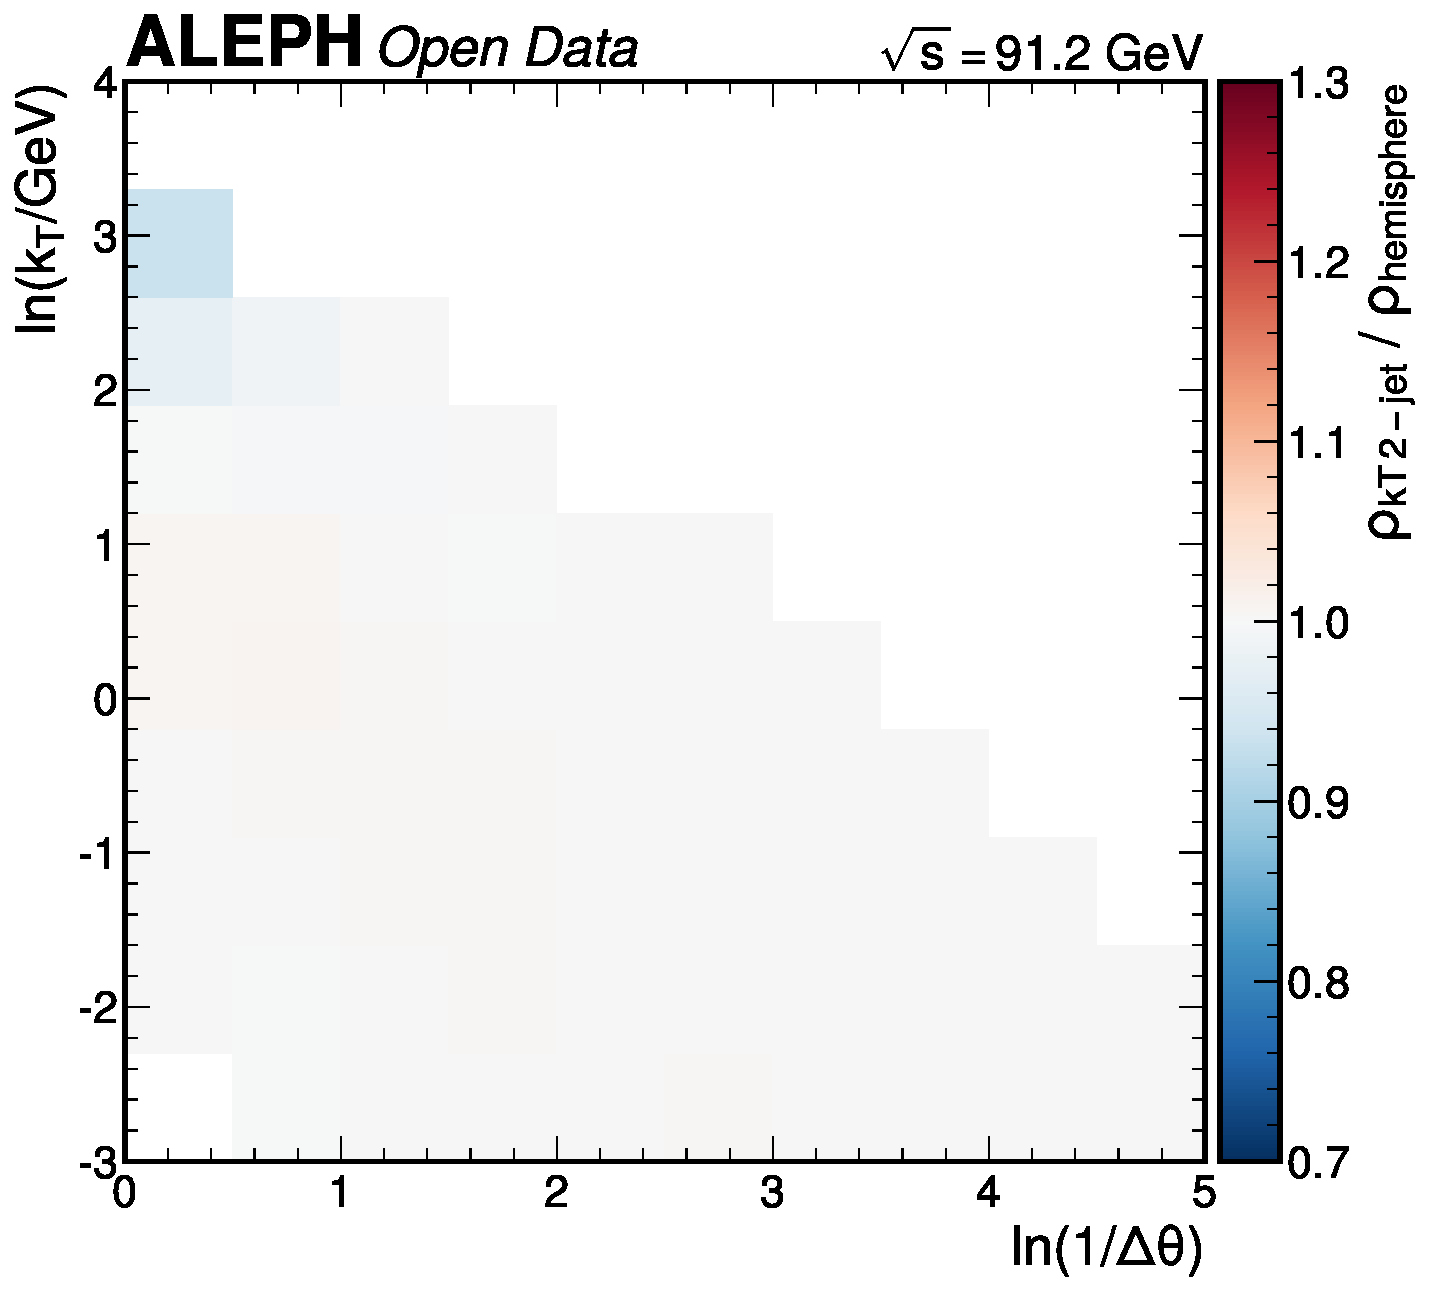
\includegraphics[height=0.38\linewidth]{figures/ingrid_approach_a_vs_c_2d.pdf}\hspace{1em}%
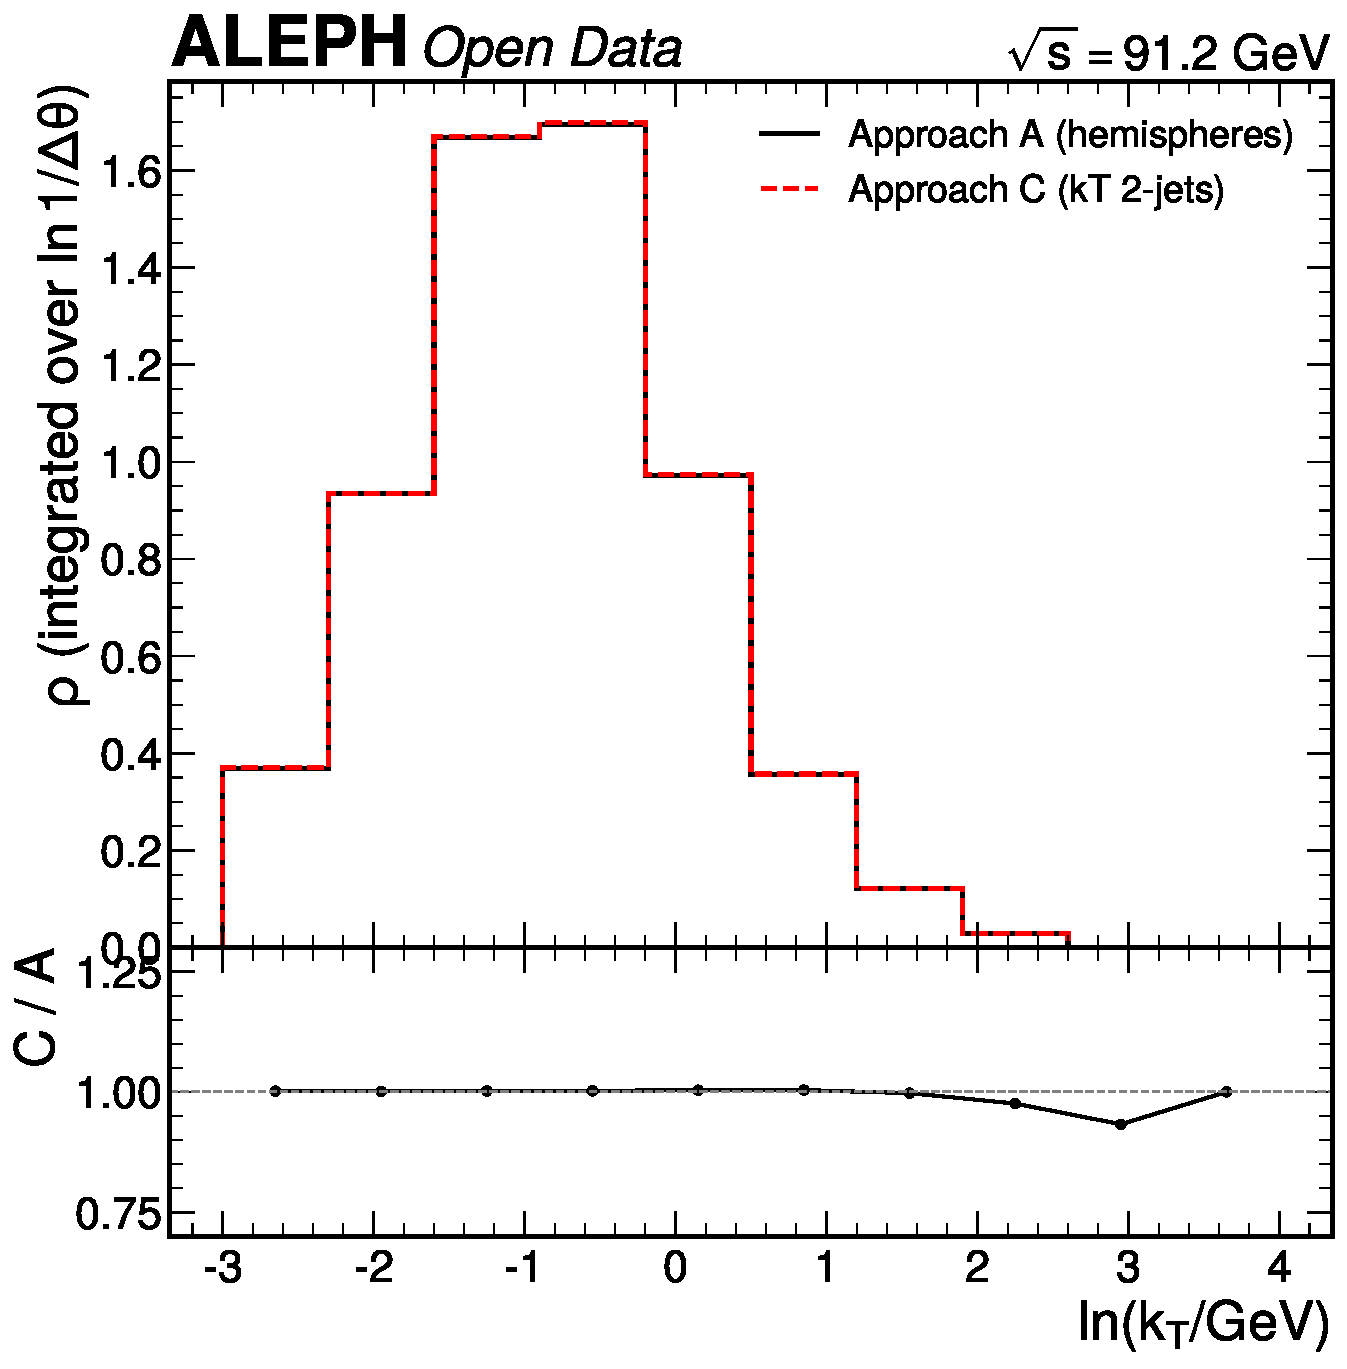
\includegraphics[height=0.38\linewidth]{figures/ingrid_approach_kt_comparison.pdf}
\caption{Comparison of Approach~A (thrust hemispheres) and Approach~C
  (Durham 2-jets).  Left: 2D ratio Approach~C / Approach~A, close to
  unity across the populated plane.  Right: $\ln k_T$ projections for
  both approaches.  The excellent agreement ($\chi^2/\text{ndf} = 0.185$)
  confirms that the Lund plane density is insensitive to the jet
  definition at this level of precision.}
\label{fig:approach-comparison}
\end{figure}

\subsection{$p_T$ vs energy ordering}
\label{sec:xcheck-ordering}

The hardness variable for subjet ordering was studied by comparing
$p_T$ ordering (primary) with energy ordering (alternative) on
MC gen-level events, as shown in Figure~\ref{fig:ordering-comparison}.
In the perturbative core
($1 < \ln(1/\Delta\theta) < 4$, $-1 < \ln k_T < 2$), the difference
is $<\!5\%$.  Larger differences (up to 15--20\%) appear at wide
angles ($\ln(1/\Delta\theta) < 1$) where the beam-axis projection
is most sensitive to the jet orientation.

\begin{figure}[htbp]
\centering
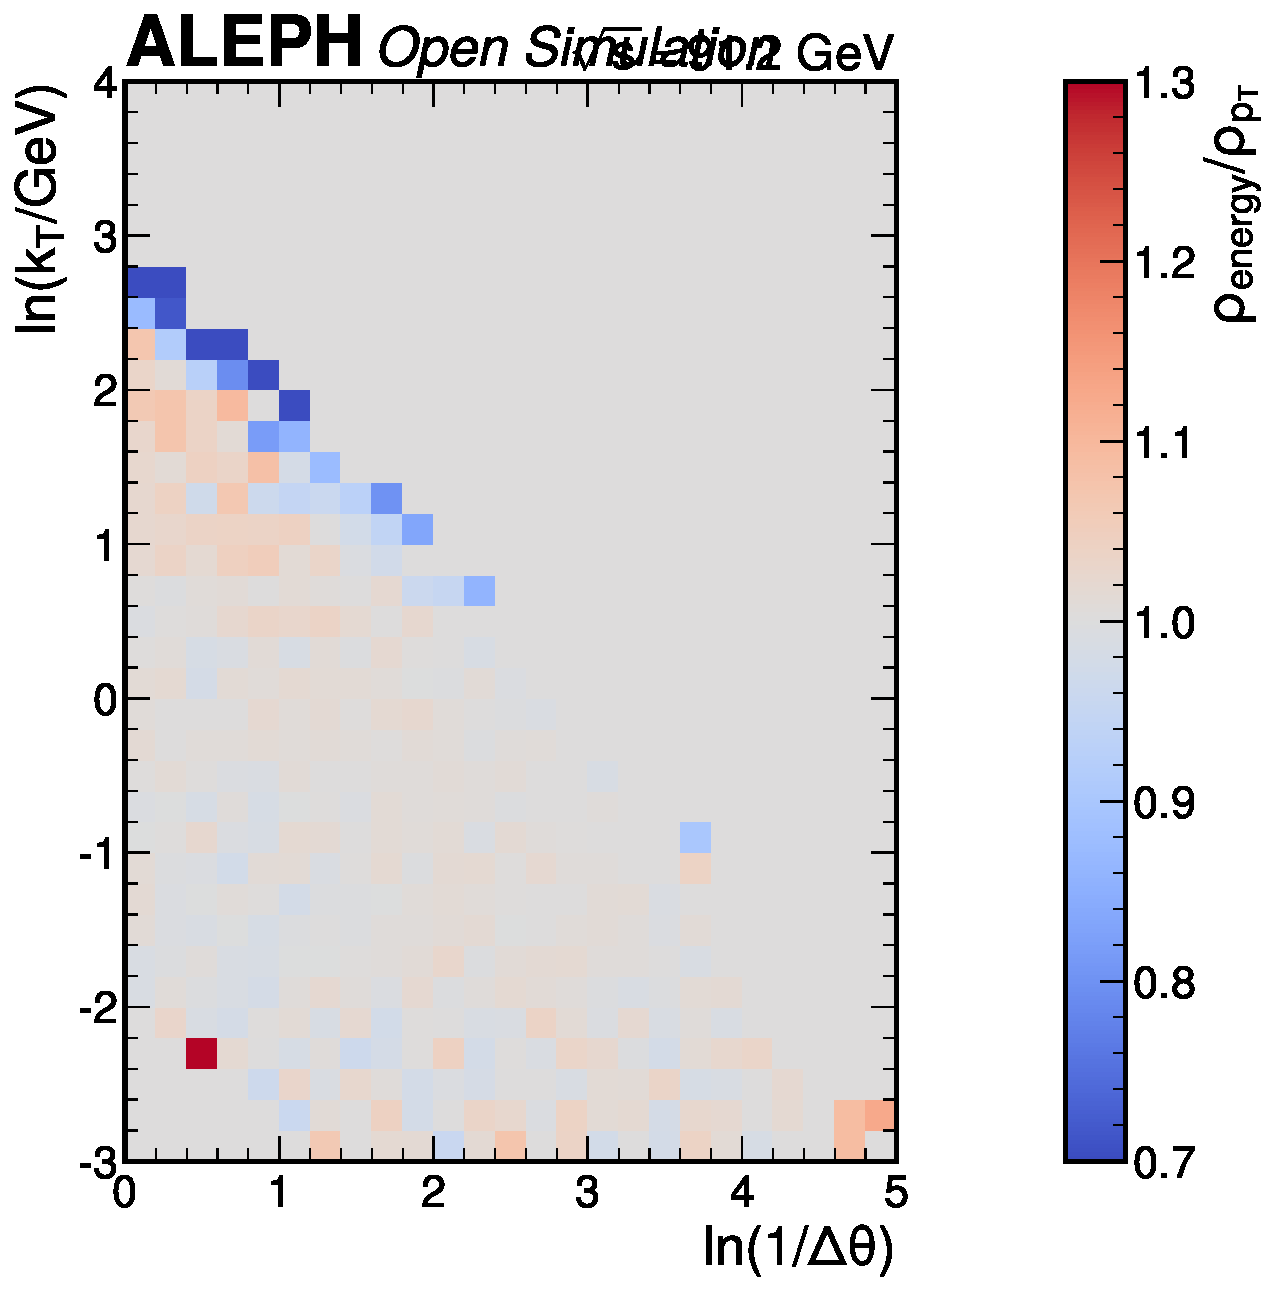
\includegraphics[height=0.38\linewidth]{figures/hugo_pt_vs_energy_ordering_ratio.pdf}\hspace{1em}%
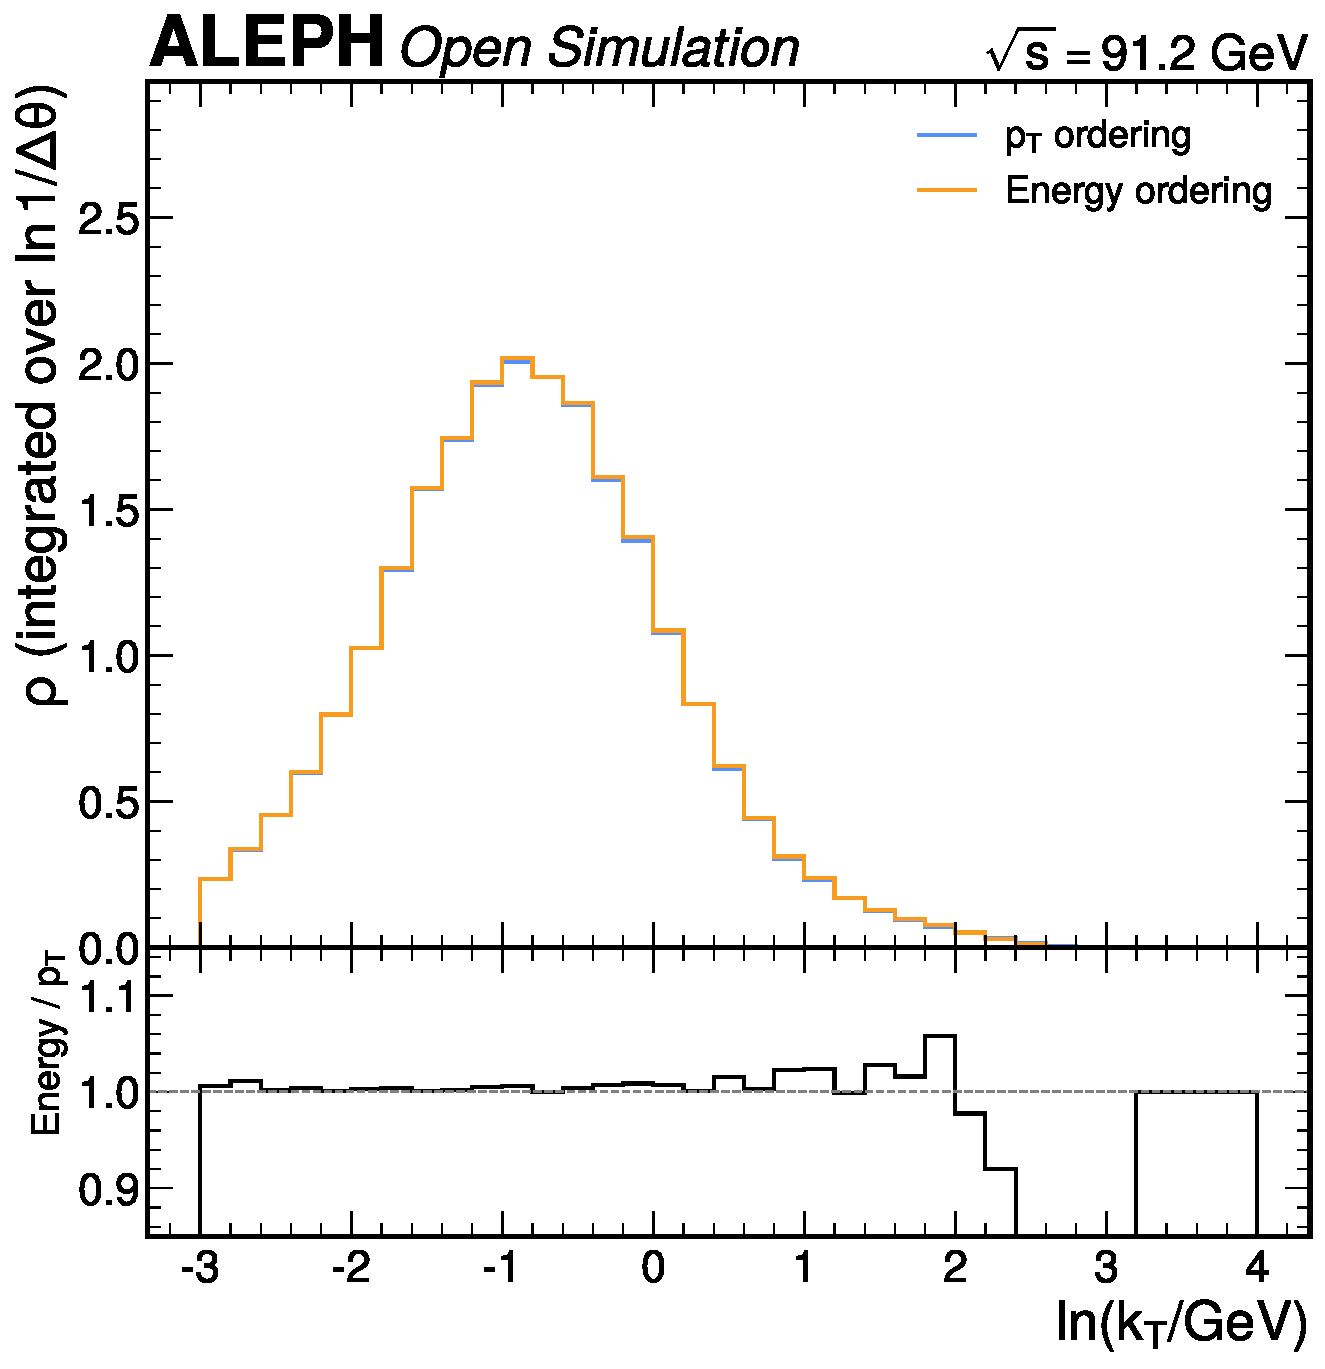
\includegraphics[height=0.38\linewidth]{figures/hugo_pt_vs_energy_kt_projection.pdf}
\caption{Comparison of $p_T$-ordered (primary) and energy-ordered
  primary declustering chains.  Left: 2D ratio energy/pT, close to
  unity in the collinear region and deviating up to 15--20\% at wide
  angles.  Right: $\ln k_T$ projection for both orderings.  The
  $p_T$ ordering is confirmed as the primary choice for
  comparability with LHC measurements; the ordering difference is
  confined to the wide-angle, non-perturbative region.}
\label{fig:ordering-comparison}
\end{figure}

\subsection{Year-by-year stability}
\label{sec:xcheck-year}

Year-to-year stability of the Lund plane was assessed via the mean
thrust and charged multiplicity across data-taking periods
(Table~\ref{tbl:year-stability}).  The maximum variation in thrust
is 0.9\% and in $N_\text{ch}$ is 1.9\%, well within statistical
expectations.  No data-taking period requires special treatment.

\subsubsection{Per-year Lund plane stability on 10\% data}
\label{sec:xcheck-year-10pct}

Each of the six data-taking periods was processed independently using
the 10\% subsample and compared to the combined 10\% result.  All
periods show excellent statistical consistency:

\begin{table}[htbp]
\centering
\caption{Per-year stability of the Lund plane $\ln k_T$ projection
  from the 10\% data subsample.  Each year is compared to the combined
  10\% result.  All $\chi^2/\text{ndf}$ values are well below 2,
  confirming no time-dependent detector effects.}
\label{tbl:year-10pct}
\begin{tabular}{lc}
\toprule
Period & $\chi^2/\text{ndf}$ ($\ln k_T$ proj.) \\
\midrule
1992 & 4.7 / 9 = 0.52 \\
1993 & 9.6 / 9 = 1.06 \\
1994 P1 & 3.0 / 9 = 0.34 \\
1994 P2 & 6.2 / 9 = 0.69 \\
1994 P3 & 3.6 / 9 = 0.40 \\
1995 & 8.6 / 9 = 0.96 \\
\bottomrule
\end{tabular}
\end{table}

The per-year $\chi^2/\text{ndf}$ values range from 0.34 to 1.06,
confirming that the Lund plane density is stable across the full
1992--1995 data-taking period.  The per-year projections are shown in
Figure~\ref{fig:10pct-year-stability}.  This stability result directly
validates the time-independence of the detector response and the
analysis chain.

\begin{figure}[htbp]
\centering
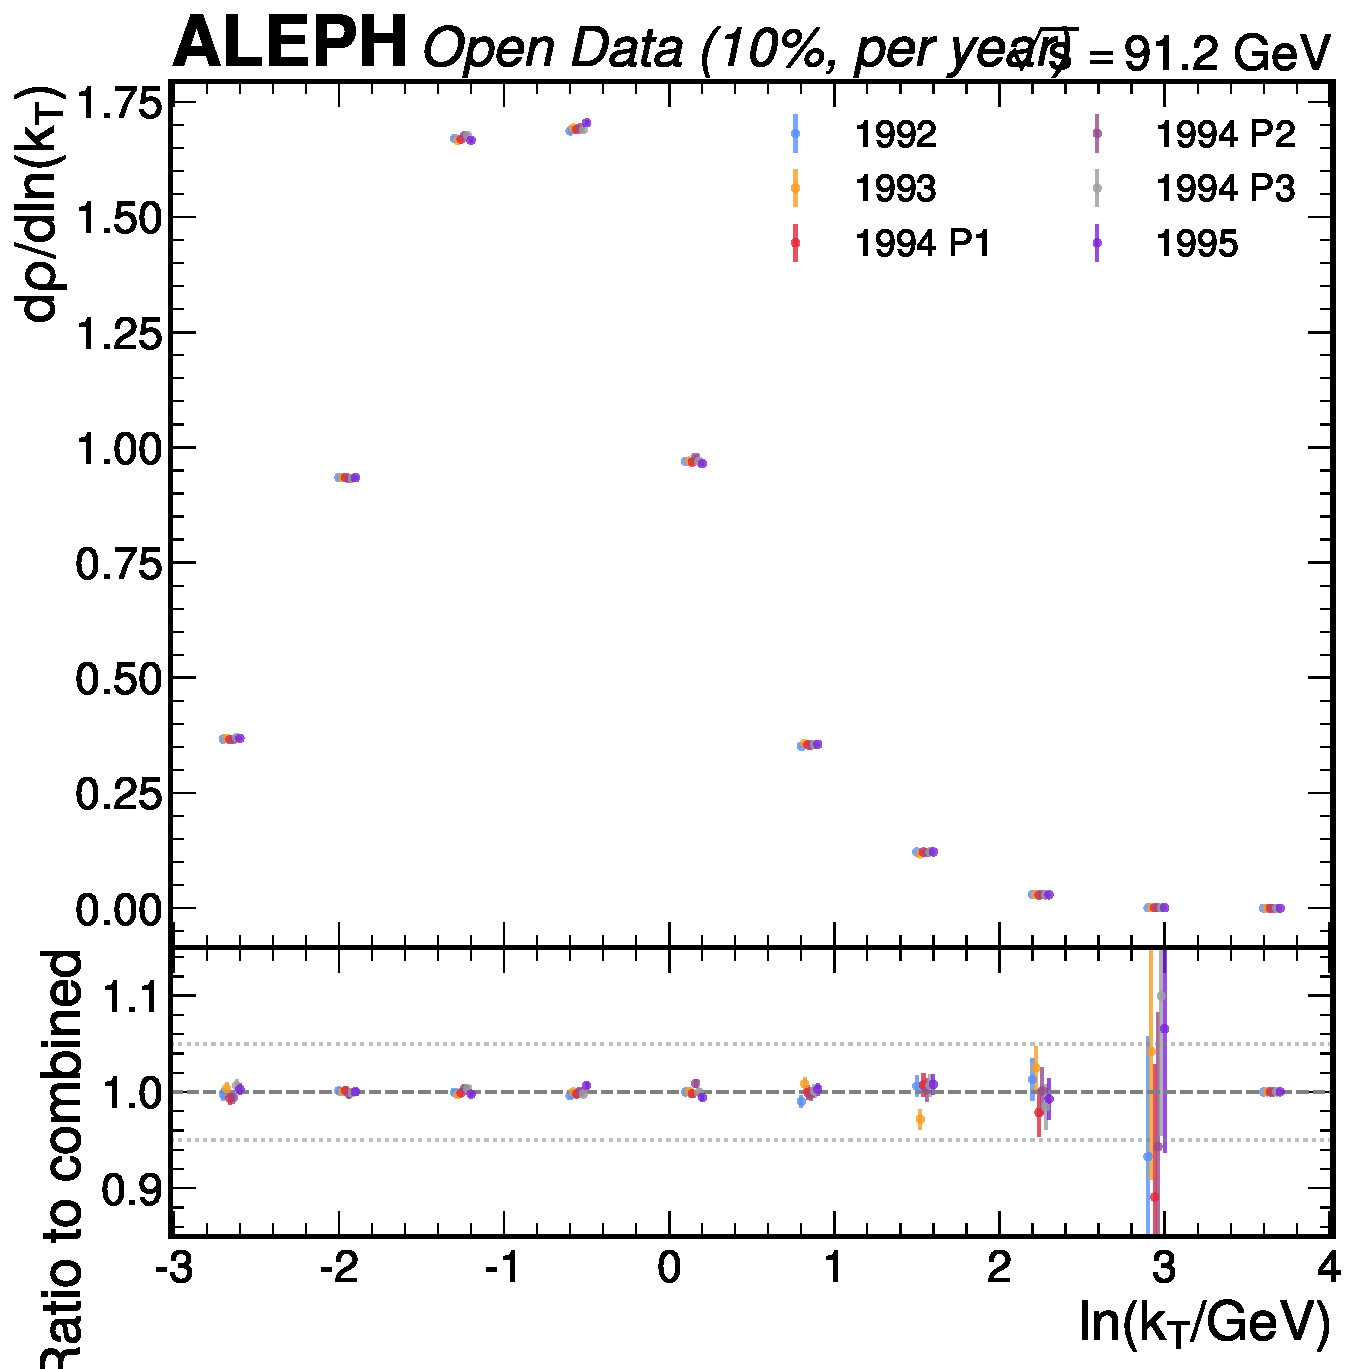
\includegraphics[width=0.47\linewidth]{figures/oscar_per_year_kt.pdf}\hspace{1em}%
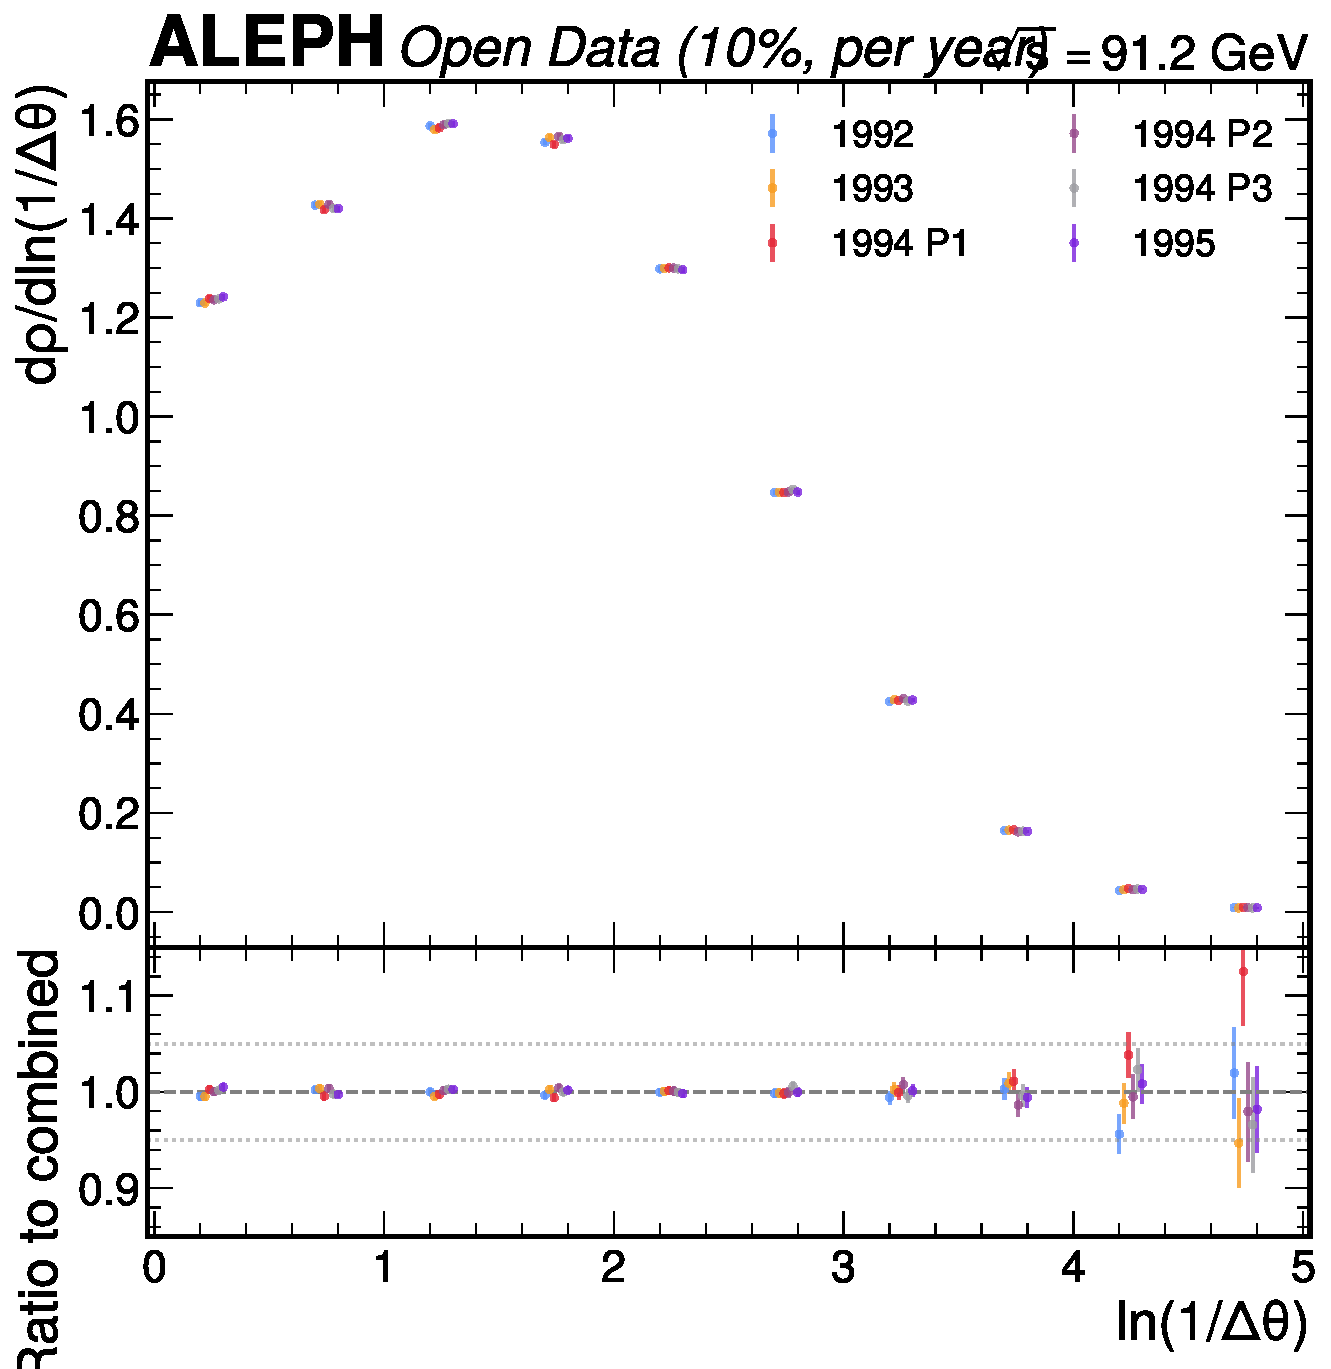
\includegraphics[width=0.47\linewidth]{figures/oscar_per_year_dtheta.pdf}
\caption{Per-year stability of the Lund plane projections from the
  10\% data subsample.  Left: $\ln k_T$ projection for each
  data-taking period.  Right: $\ln(1/\Delta\theta)$ projection.
  The bottom panels show the ratio to the combined 10\% result.
  All six periods are consistent with the combined result within
  $\pm 5\%$, and the $\chi^2/\text{ndf}$ is below 1.1 for every
  period (Table~\ref{tbl:year-10pct}).}
\label{fig:10pct-year-stability}
\end{figure}

% =====================================================================
% 7. STATISTICAL METHOD
% =====================================================================
\section{Statistical Method}
\label{sec:statmethod}

\subsection{Bootstrap covariance}
\label{sec:bootstrap}

The statistical covariance matrix is constructed via event-level
bootstrap with $N = 500$ replicas.  Each replica:
\begin{enumerate}
\item Resamples reco events with replacement.
\item Resamples genBefore events with replacement.
\item Recomputes correction factors
  $C_\text{rep} = N_\text{genBefore}^\text{rep} /
  N_\text{reco}^\text{rep}$.
\item Applies the resampled correction to the resampled reco.
\item Computes the corrected Lund plane density.
\end{enumerate}

The covariance matrix is then (Eq.~\eqref{eq:bootstrap-cov})
\begin{equation}
  V_{ij}^\text{stat} = \frac{1}{N-1}
  \sum_{r=1}^{N}
  \left(\rho_i^{(r)} - \bar{\rho}_i\right)
  \left(\rho_j^{(r)} - \bar{\rho}_j\right),
  \label{eq:bootstrap-cov}
\end{equation}
where $\rho_i^{(r)}$ is the density in bin $i$ for replica $r$ and
$\bar{\rho}_i$ is the mean across replicas.  This captures the full
statistical correlation structure, including correlations from shared
correction-factor denominators and self-normalization.

\subsection{Systematic covariance}
\label{sec:syst-cov}

Each systematic source $k$ contributes a covariance matrix
(Eq.~\eqref{eq:syst-cov}) from the outer product of the symmetrised
shift vector:
\begin{equation}
  V_{ij}^{(k)} = \delta_i^{(k)} \cdot \delta_j^{(k)}\,,
  \label{eq:syst-cov}
\end{equation}
where $\delta_i^{(k)} = (\delta_i^{(k,\text{up})} -
\delta_i^{(k,\text{down})}) / 2$ is the symmetrised shift in bin $i$.

\subsection{Total covariance and $\chi^2$}
\label{sec:total-cov}

The total covariance matrix is
$V^\text{total} = V^\text{stat} + \sum_k V^{(k)}$.
The $\chi^2$ for comparison of two distributions
(Eq.~\eqref{eq:chi2}) is
\begin{equation}
  \chi^2 = (\mathbf{d} - \mathbf{m})^T\;
  (V^\text{total})^{-1}\;
  (\mathbf{d} - \mathbf{m})\,,
  \label{eq:chi2}
\end{equation}
where $\mathbf{d}$ and $\mathbf{m}$ are the data and model density
vectors restricted to the 58 populated bins.

The covariance matrix is verified to be positive semi-definite (all
eigenvalues $\ge 0$) with condition number $< 10^{10}$.

\begin{figure}[htbp]
\centering
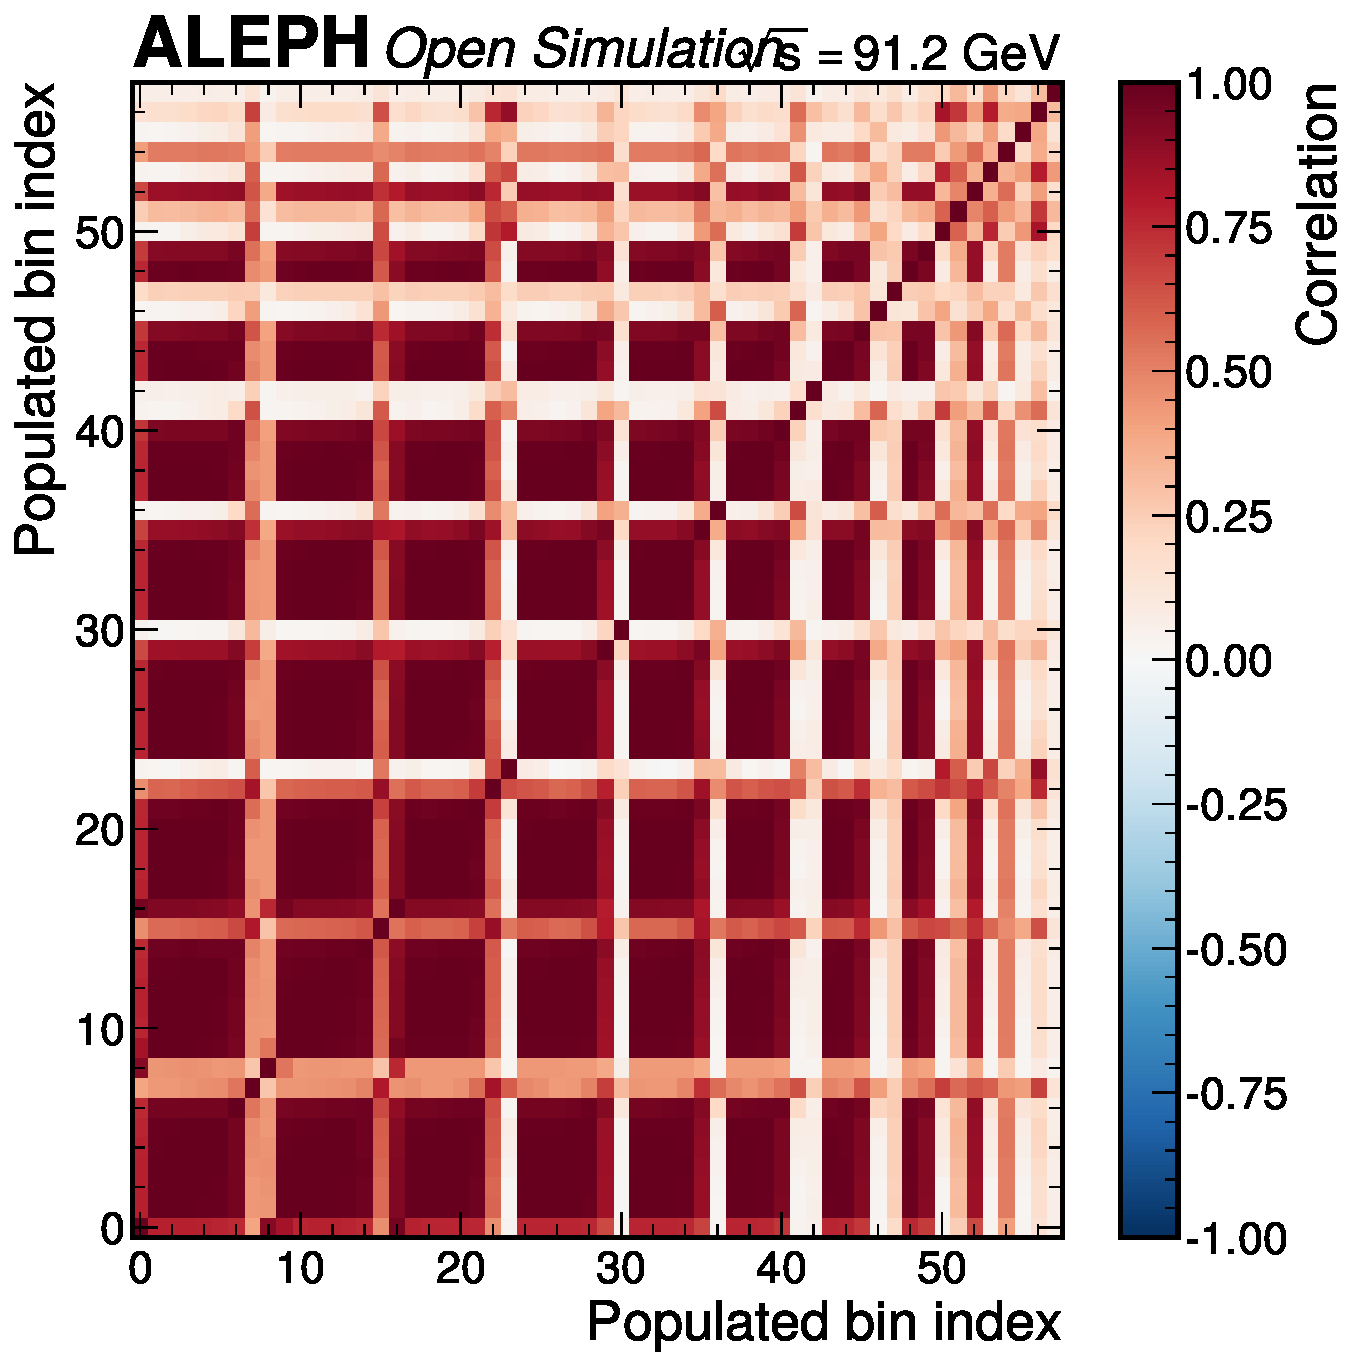
\includegraphics[width=0.55\linewidth]{figures/nikolai_correlation_matrix.pdf}
\caption{Correlation matrix for the 58 populated bins of the Lund
  plane, computed from the total (statistical + systematic) covariance.
  The diagonal elements are unity by construction.  Off-diagonal
  correlations arise primarily from the MC model dependence systematic
  (which shifts the full plane coherently) and from the bootstrap
  statistical covariance (which introduces correlations from the
  self-normalization).  The correlation structure is dominated by
  nearby-bin positive correlations from detector resolution effects.}
\label{fig:correlation-matrix}
\end{figure}

% =====================================================================
% 8. RESULTS
% =====================================================================
\section{Results}
\label{sec:results}

% =====================================================================
% 8.1 PRIMARY RESULT: Corrected full-data 2D Lund plane
% =====================================================================
\subsection{Corrected 2D Lund plane density (primary result)}
\label{sec:primary-result}

Figure~\ref{fig:lund-full} presents the corrected primary Lund jet plane
density from the full ALEPH dataset.  This is the flagship result of the
analysis---the first full two-dimensional primary Lund jet plane density
measurement in $e^+e^-$ collisions.

The full ALEPH dataset (Table~\ref{tbl:full-summary}) is processed using
the identical analysis chain validated on the 10\% subsample
(Section~\ref{sec:results-10pct}).  All six data files covering the
1992--1995 data-taking period are processed without subsampling.

\begin{table}[htbp]
\centering
\caption{Full data processing summary.  Selection efficiencies are
  uniform across years (93.2--93.5\%), consistent with the MC reco
  efficiency (93.5\%) and with the 10\% subsample result.}
\label{tbl:full-summary}
\begin{tabular}{lcc}
\toprule
Quantity & Full data & MC reco \\
\midrule
Raw events & 3\,050\,610 & 771\,597 \\
After selection & 2\,868\,384 & 726\,585 \\
After hemi cut & 2\,846\,194 & 721\,175 \\
Hemispheres & 5\,692\,388 & 1\,442\,350 \\
Primary splittings & 28\,934\,792 & 7\,405\,085 \\
Splittings/hemisphere & 5.083 & 5.134 \\
Selection efficiency & 93.3\% & 93.5\% \\
\bottomrule
\end{tabular}
\end{table}

The bin-by-bin correction factors from the full MC (40~files, Phase~3)
are applied to the full data (Table~\ref{tbl:full-correction}).
The correction factors
$C(i,j) = N_\text{genBefore}(i,j) / N_\text{reco}(i,j)$ range from 1.17
to 6.67, identical to those used in the expected and 10\% results.

\begin{table}[htbp]
\centering
\caption{Full-data correction summary.}
\label{tbl:full-correction}
\begin{tabular}{lc}
\toprule
Quantity & Value \\
\midrule
Data hemispheres & 5\,692\,388 \\
Corrected hemispheres & 7\,643\,440 \\
$R_\text{hemi} = N_\text{hemi}^\text{genBefore} / N_\text{hemi}^\text{reco}$ & 1.3427 \\
Populated bins & 58 / 100 \\
Total corrected splittings & 34\,473\,358 \\
\bottomrule
\end{tabular}
\end{table}

\begin{figure}[htbp]
\centering
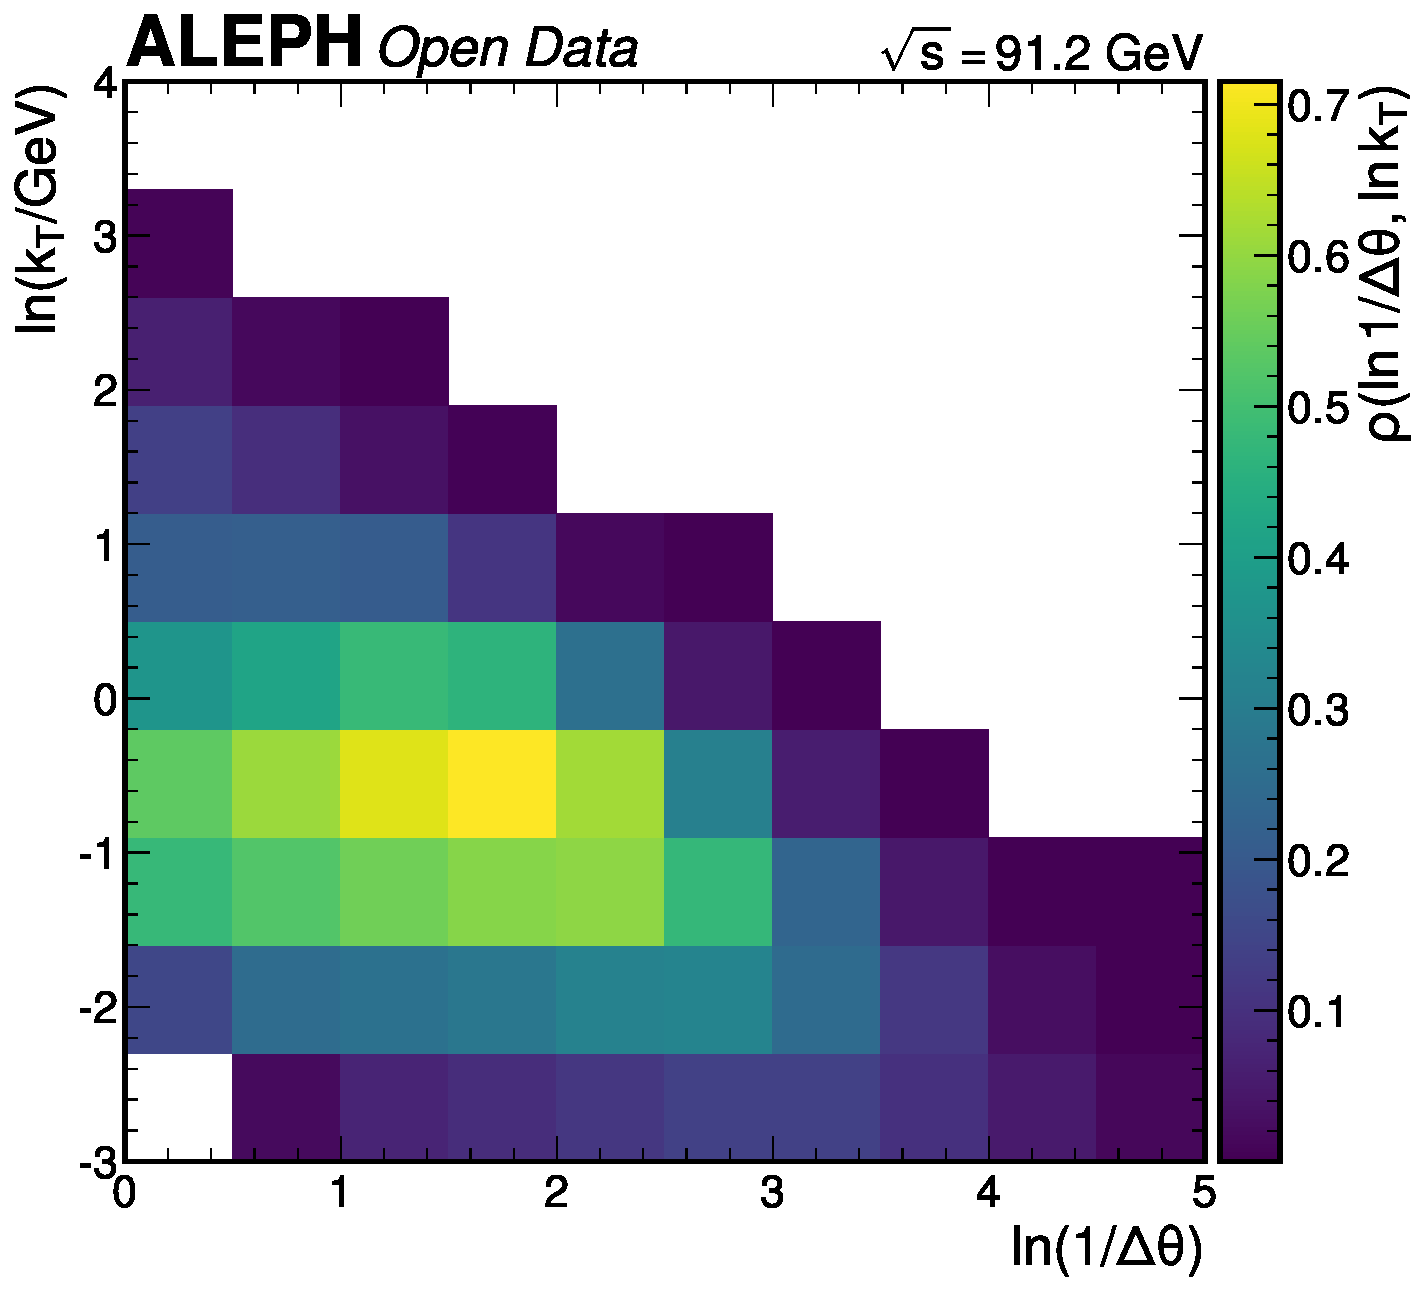
\includegraphics[width=0.55\linewidth]{figures/emeric_lund_plane_full_corrected.pdf}
\caption{Corrected primary Lund jet plane density
  $\rho(\ln(1/\Delta\theta), \ln(k_T/\text{GeV}))$ at charged-particle
  level, from the full ALEPH dataset ($5\,692\,388$ hemispheres,
  corrected to $7\,643\,440$).  The characteristic triangular
  structure is clearly resolved: the kinematic boundary (upper-left
  triangle) is depopulated, the perturbative plateau at moderate
  $\ln(1/\Delta\theta)$ and $\ln k_T$ has density $\sim\!0.06$--$0.08$,
  the non-perturbative rise at $\ln k_T < -1$ reflects hadronization,
  and the collinear enhancement at large $\ln(1/\Delta\theta)$ shows
  the soft-collinear divergence.  The maximum density of $\sim\!0.72$
  occurs at $(\ln(1/\Delta\theta), \ln k_T) \approx (1.5, -0.55)$.
  This figure represents the primary result of this analysis.}
\label{fig:lund-full}
\end{figure}

The Lund plane shows the expected triangular kinematic boundary.  The
density peaks at $\rho \approx 0.72$ in the region
$\ln(1/\Delta\theta) \approx 1.5$, $\ln k_T \approx -0.55$
(moderate-angle, soft radiation).  The density falls steeply toward the
kinematic boundary and at large angles.  The perturbative plateau
($1 < \ln(1/\Delta\theta) < 4$, $\ln k_T > 1$) has density
$\rho \approx 0.05$--$0.08$, consistent with the leading-order QCD
prediction $\rho_\text{LO}^\text{charged} \approx 0.067$
(Eq.~\ref{eq:rho-lo}).

Figure~\ref{fig:lund-full-annotated} shows the same result with
per-bin density values and total uncertainties annotated.
The normalization is verified in Table~\ref{tbl:normalization}.

\begin{figure}[htbp]
\centering
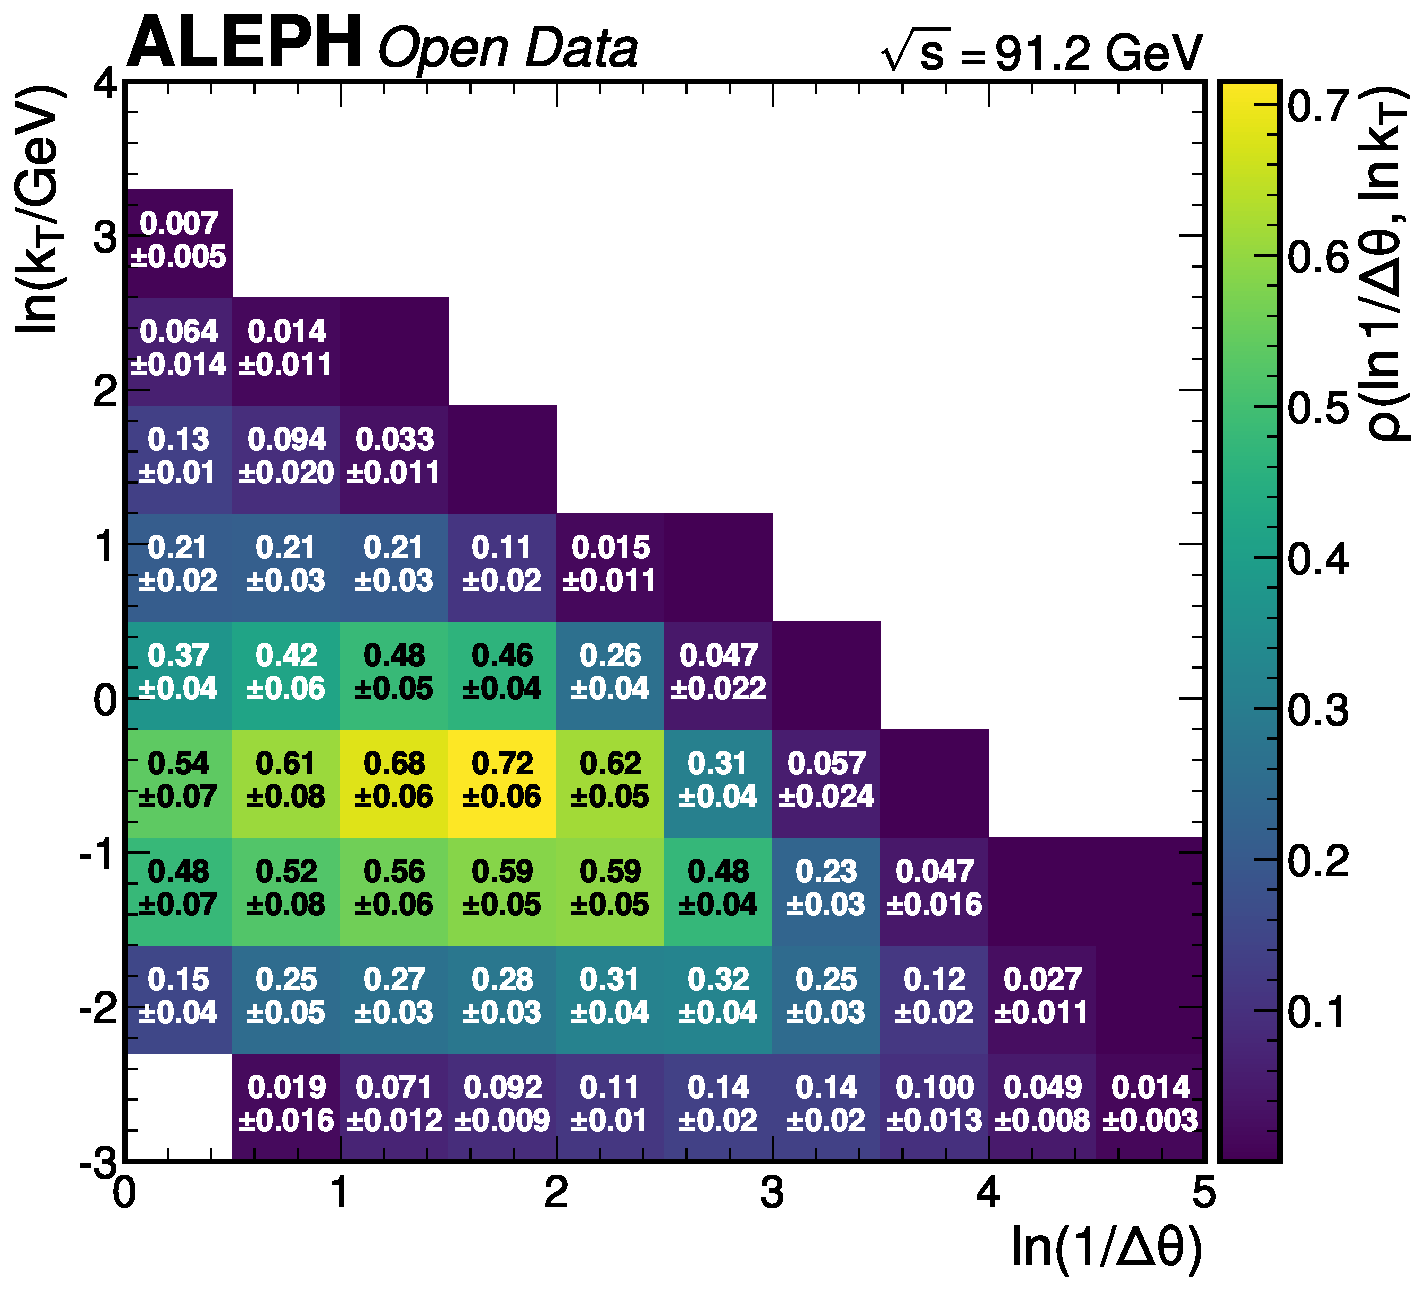
\includegraphics[width=0.55\linewidth]{figures/emeric_lund_plane_full_annotated.pdf}
\caption{Corrected Lund plane density from full data with per-bin
  numerical values annotated as $\rho \pm \sigma_\text{tot}$.  Values
  are shown for the 50 bins with density $> 0.005$; the 8 remaining
  boundary bins with smaller populations are omitted for clarity.
  The 58 populated bins span four orders
  of magnitude in density, from $\sim\!10^{-5}$ at the extreme
  kinematic boundaries to $\sim\!0.72$ at the non-perturbative peak.}
\label{fig:lund-full-annotated}
\end{figure}

\begin{table}[htbp]
\centering
\caption{Normalization verification across analysis phases.  The integral
  $\int \rho\,\Delta x\,\Delta y$ represents the mean number of primary
  Lund splittings per hemisphere.  All three results agree within
  $\sim\!1\%$, well within the $\sim\!5\%$ MC model dependence systematic.}
\label{tbl:normalization}
\begin{tabular}{lccc}
\toprule
Quantity & Full data & 10\% data & MC expected \\
\midrule
$\int \rho\,dA$ (splits/hemi) & 4.510 & 4.511 & 4.562 \\
Deficit vs MC & $-1.1\%$ & $-1.1\%$ & --- \\
\bottomrule
\end{tabular}
\end{table}

The leading-order QCD prediction for the perturbative density
is~\cite{Dreyer:2018nbf}
\begin{equation}
  \rho_\text{LO} = \frac{2\,\alpha_s(k_T)\,C_F}{\pi}\,,
  \label{eq:rho-lo}
\end{equation}
where $C_F = 4/3$ for quark-initiated jets.  Using
$\alpha_s(M_Z) = 0.1180 \pm 0.0009$~\cite{ParticleDataGroup:2024cfk},
this gives $\rho_\text{LO}^\text{all-part} \approx 0.100$ for all
particles and $\rho_\text{LO}^\text{charged} \approx 0.067$ for charged
particles (a factor of $\sim\!2/3$ from the charged fraction of the
hadron multiplicity).

% =====================================================================
% 8.2 1D PROJECTIONS (full data, with LO overlay)
% =====================================================================
\subsection{1D projections}
\label{sec:results-1d}

The $\ln k_T$ and $\ln(1/\Delta\theta)$ projections provide the
one-dimensional spectra that are most directly comparable to prior
measurements and analytical predictions (Figure~\ref{fig:full-1d}).
These projections integrate the two-dimensional density $\rho(x,y)$
over one coordinate:
\begin{equation*}
  \frac{d\rho}{d(\ln k_T)} = \int \rho\,d\!\left(\ln\frac{1}{\Delta\theta}\right),
  \qquad
  \frac{d\rho}{d(\ln 1/\Delta\theta)} = \int \rho\,d(\ln k_T).
\end{equation*}

\begin{figure}[htbp]
\centering
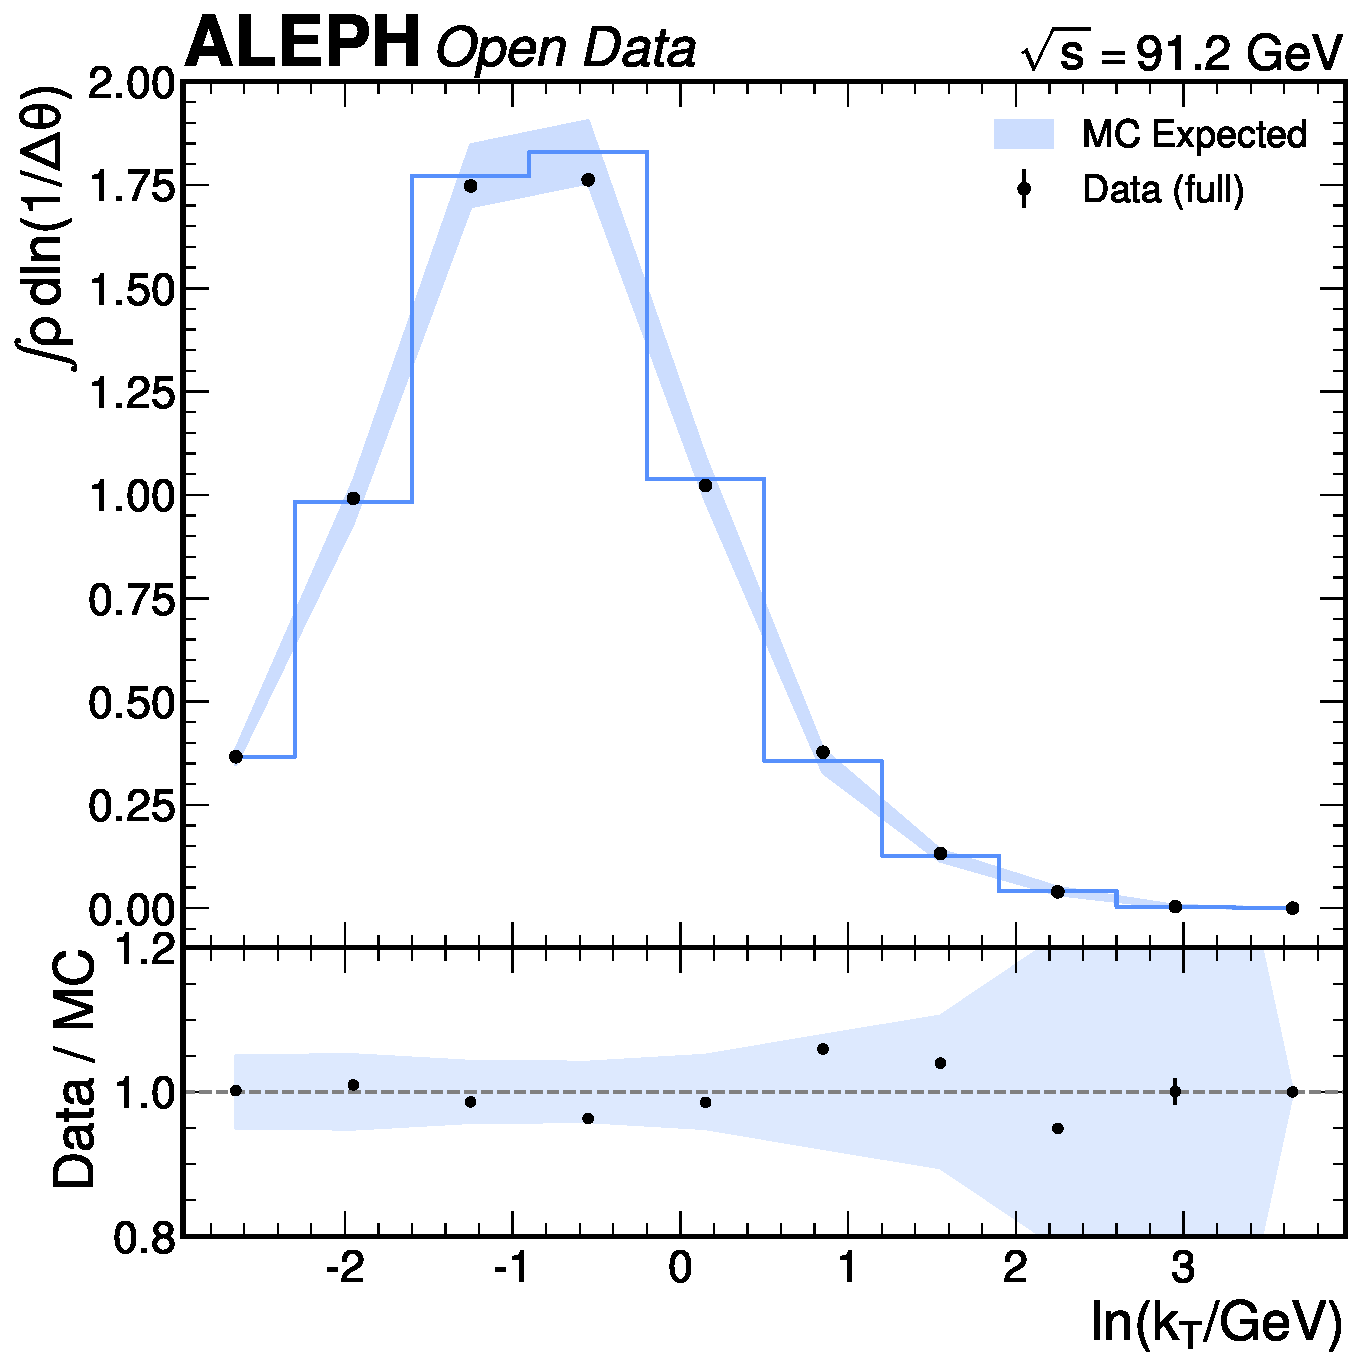
\includegraphics[height=0.38\linewidth]{figures/emeric_1d_kt_projection.pdf}\hspace{1em}%
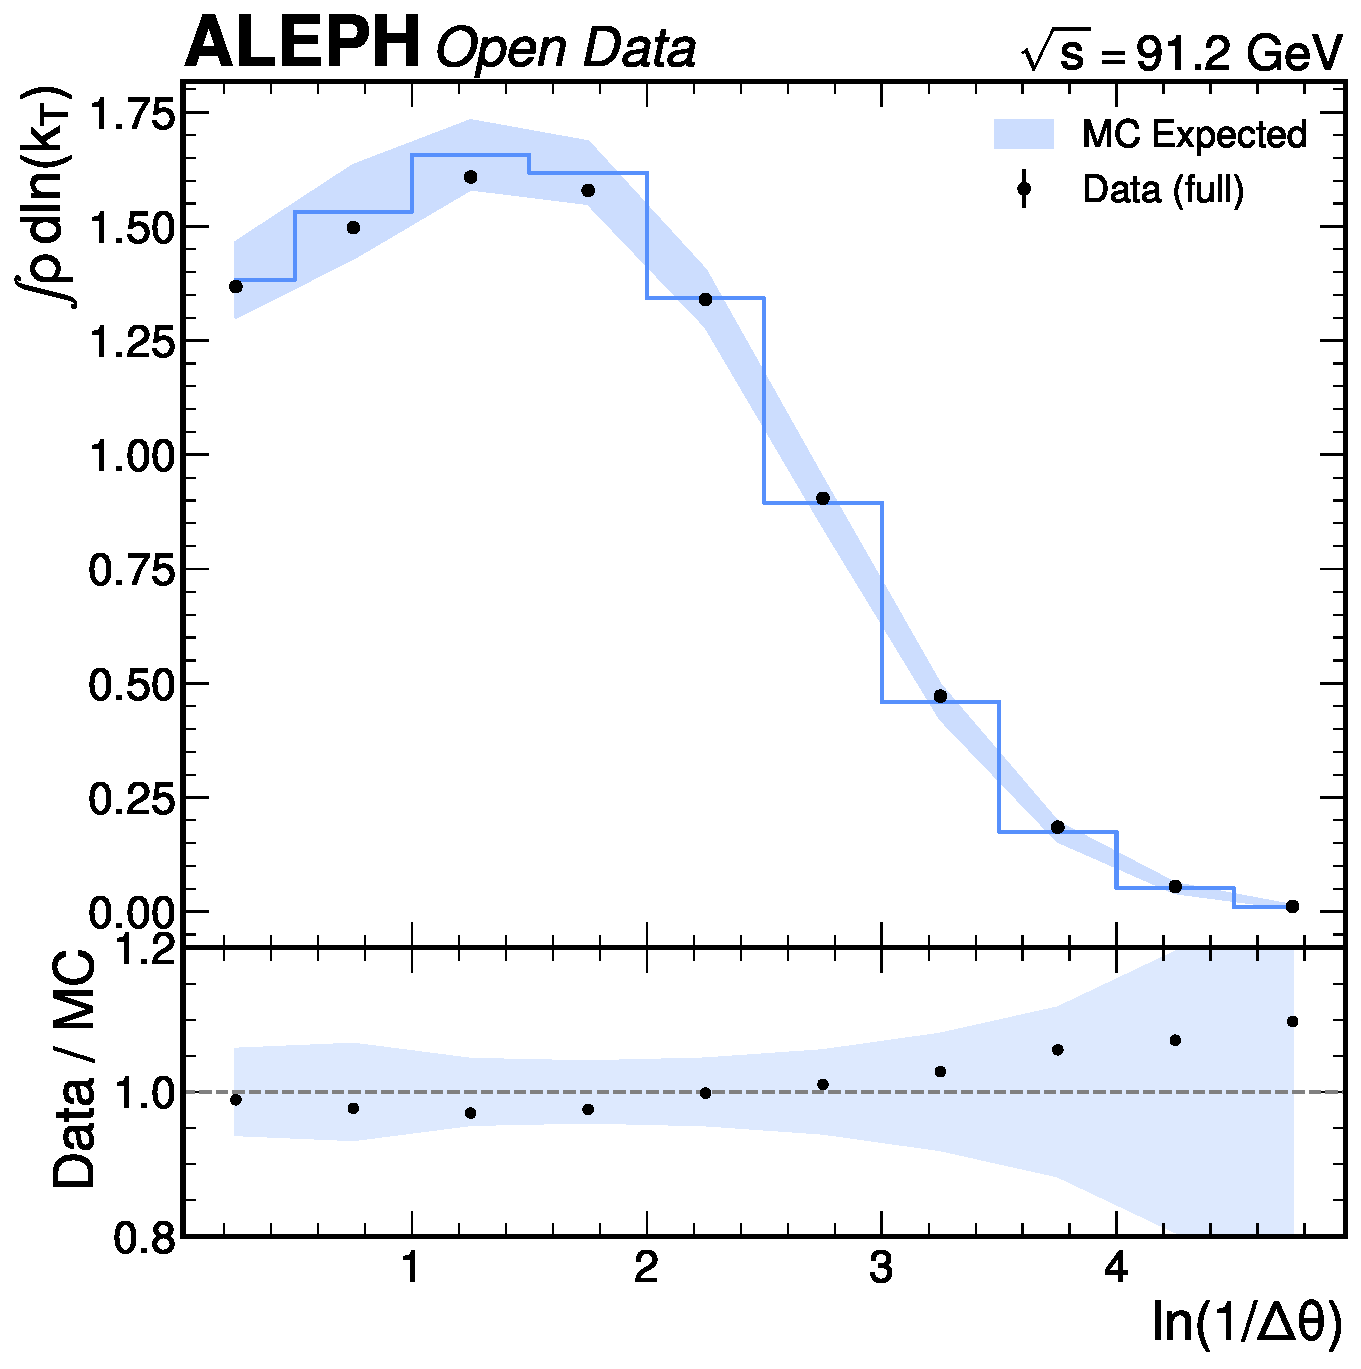
\includegraphics[height=0.38\linewidth]{figures/emeric_1d_dtheta_projection.pdf}
\caption{1D projections of the corrected Lund plane density from the
  full dataset (black points with statistical error bars) compared to
  the MC expected result (blue band showing stat + syst uncertainty).
  Left: $\ln k_T$ projection.  The peak at $\ln k_T \sim -1$ ($k_T
  \sim 0.37$~GeV) is consistent with the soft radiation peak from
  hadronization.  Data and MC agree within the uncertainty band across
  the full range.  Right: $\ln(1/\Delta\theta)$ projection.  The broad
  peak at $\ln(1/\Delta\theta) \sim 1.0$--$1.5$ and the steeply
  falling tail at large angles are well-reproduced by the MC.  The
  ratio panels confirm agreement within $\pm 5\%$ across both
  projections.}
\label{fig:full-1d}
\end{figure}

The $\ln k_T$ projection exhibits the characteristic QCD shape: a broad
non-perturbative peak at $\ln k_T \sim -1$ ($k_T \sim 0.37$~GeV), a
transition region around $\ln k_T \sim 0$, and a perturbative tail at
$\ln k_T > 1$.  The $\ln(1/\Delta\theta)$ projection peaks at
$\ln(1/\Delta\theta) \sim 1.0$--$1.5$ and falls steeply at both
extremes.  In both projections, the full-data points fall within the MC
uncertainty band.

Figure~\ref{fig:corrected-kt-lo} overlays the LO analytical predictions
on the corrected $\ln k_T$ projection.  The LO prediction for the
perturbative plateau, $\rho_\text{LO}^\text{charged} \approx 0.067$
(Eq.~\ref{eq:rho-lo} scaled by $\sim\!2/3$ for the charged-particle
fraction), multiplied by the full $\ln(1/\Delta\theta)$ integration
range $\Delta\!\ln(1/\Delta\theta) = 5$, gives a reference level of
$\sim\!0.34$ for the $\ln k_T$ projection in the perturbative regime.
The measured projection at high $k_T$ ($\ln k_T > 1$) is consistent
with this prediction, confirming that the leading-order colour-factor
structure is correctly reproduced by the corrected data.

\begin{figure}[htbp]
\centering
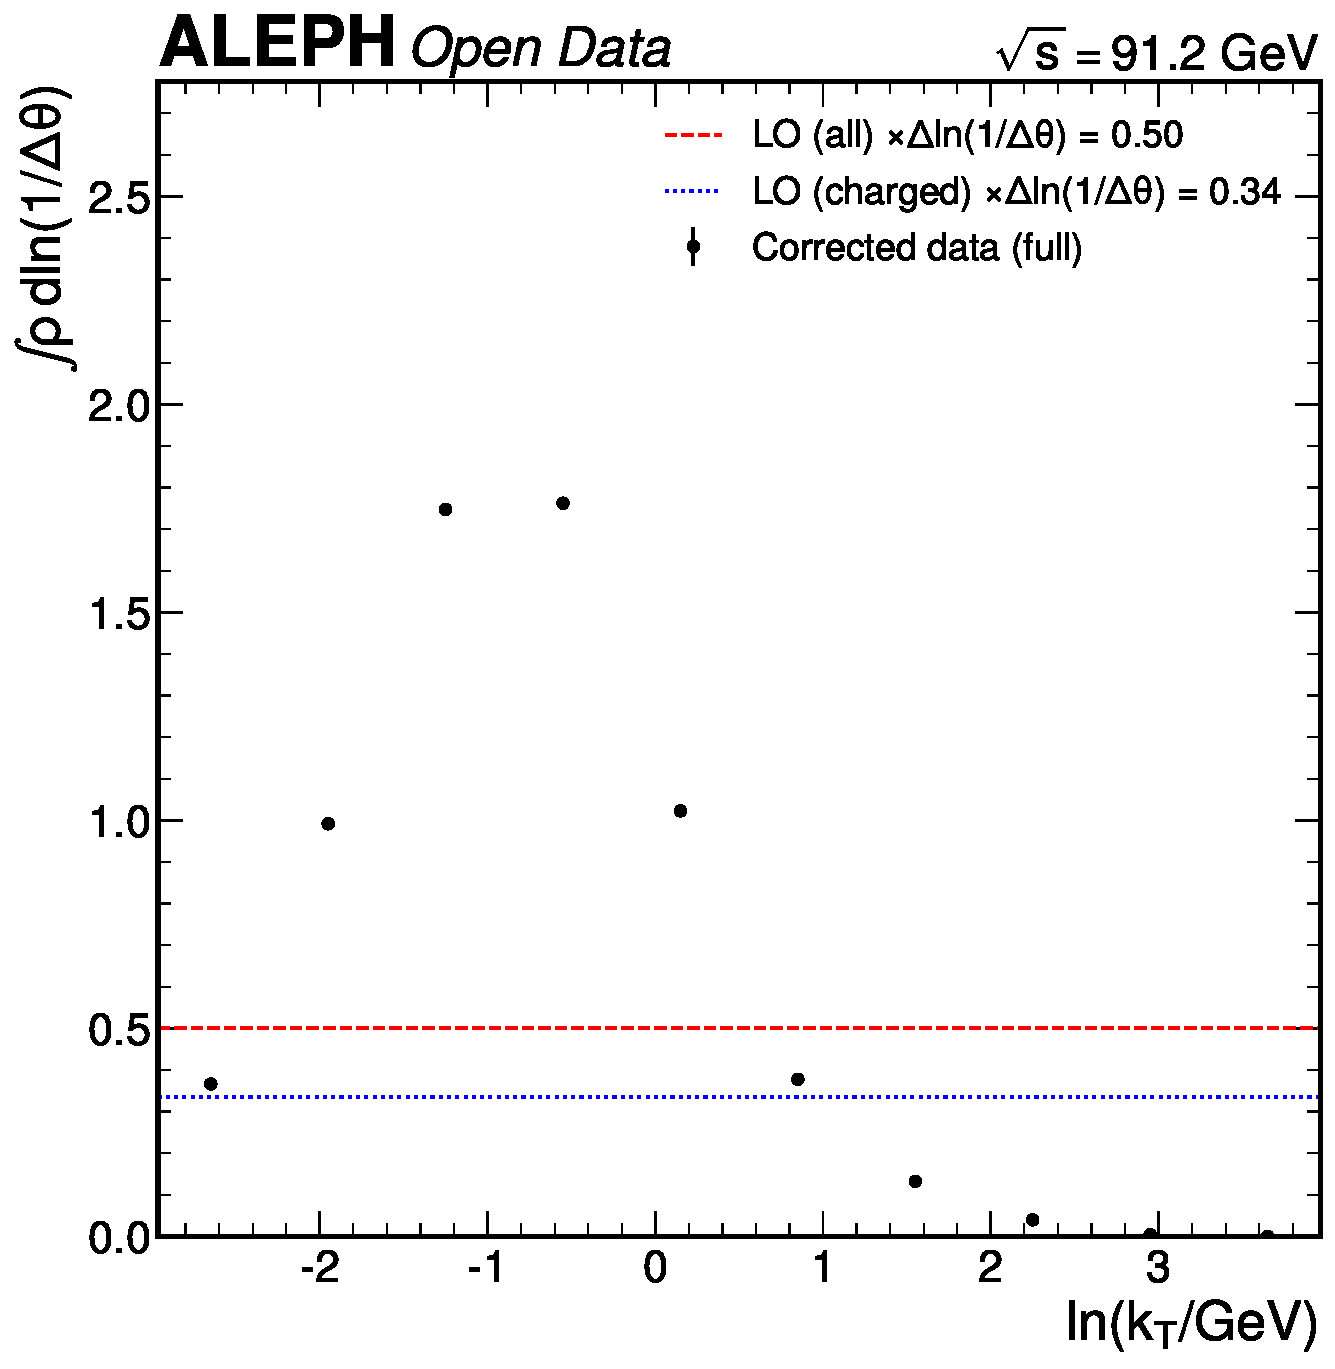
\includegraphics[width=0.55\linewidth]{figures/quentin_corrected_kt_with_lo.pdf}
\caption{Corrected $\ln k_T$ projection from the full dataset (black
  points) with LO analytical prediction reference lines.  The dashed
  red line shows $\rho_\text{LO}^\text{all-part} \times
  \Delta\!\ln(1/\Delta\theta) \approx 0.50$ and the dotted blue line
  shows $\rho_\text{LO}^\text{charged} \times
  \Delta\!\ln(1/\Delta\theta) \approx 0.34$.  The measured density at
  $\ln k_T > 1$ (perturbative regime) is consistent with the
  charged-particle LO expectation.  At $\ln k_T < 0$, the density
  exceeds the LO prediction, reflecting non-perturbative hadronization
  contributions.}
\label{fig:corrected-kt-lo}
\end{figure}

% =====================================================================
% 8.3 UNCERTAINTY BREAKDOWN
% =====================================================================
\subsection{Uncertainty breakdown}
\label{sec:results-uncertainty}

The total uncertainty on the measured Lund plane density receives
contributions from both statistical and systematic sources.
Figure~\ref{fig:uncertainty-summary} shows the relative uncertainty
as a function of $\ln k_T$ bin, averaged over $\ln(1/\Delta\theta)$
bins within each $k_T$ slice.

The statistical uncertainty is determined by the data sample size
and ranges from $\sim\!1\%$ in the most populated bins
($\ln k_T \in [-1, 0]$, where the hadronization peak produces the
highest density) to $\sim\!5$--$8\%$ at the kinematic boundaries
($\ln k_T > 2$ and $\ln k_T < -2$) where few splittings are
reconstructed.  The statistical contribution is subdominant in
the bulk of the Lund plane.

The systematic uncertainty dominates in the core of the plane and
is driven primarily by the MC model dependence systematic
(Section~\ref{sec:syst-model}), which evaluates the sensitivity
of the correction factors to the underlying physics model by
applying a 20\% two-dimensional tilt reweighting.  The second-largest
contribution comes from the tracking efficiency variation
(Section~\ref{sec:syst-tracking}), which is most significant at
low $k_T$ where soft tracks are near the reconstruction threshold.
Contributions from momentum resolution, angular resolution, and
event selection variations are individually subdominant (each
$<\!1\%$ relative) but collectively contribute $\sim\!1$--$2\%$ in
the non-perturbative region.

The total uncertainty, computed as the quadrature sum of statistical
and systematic contributions (using the full covariance matrix from
Section~\ref{sec:total-cov}), ranges from $\sim\!1\%$ in the most
populated bins to $\sim\!8\%$ at the kinematic boundaries.  The
systematic-to-statistical ratio is approximately 2:1 in the bulk,
indicating that this measurement would benefit from alternative
generator MC samples to reduce the dominant model-dependence
systematic (see Section~\ref{sec:future}).

\begin{figure}[htbp]
\centering
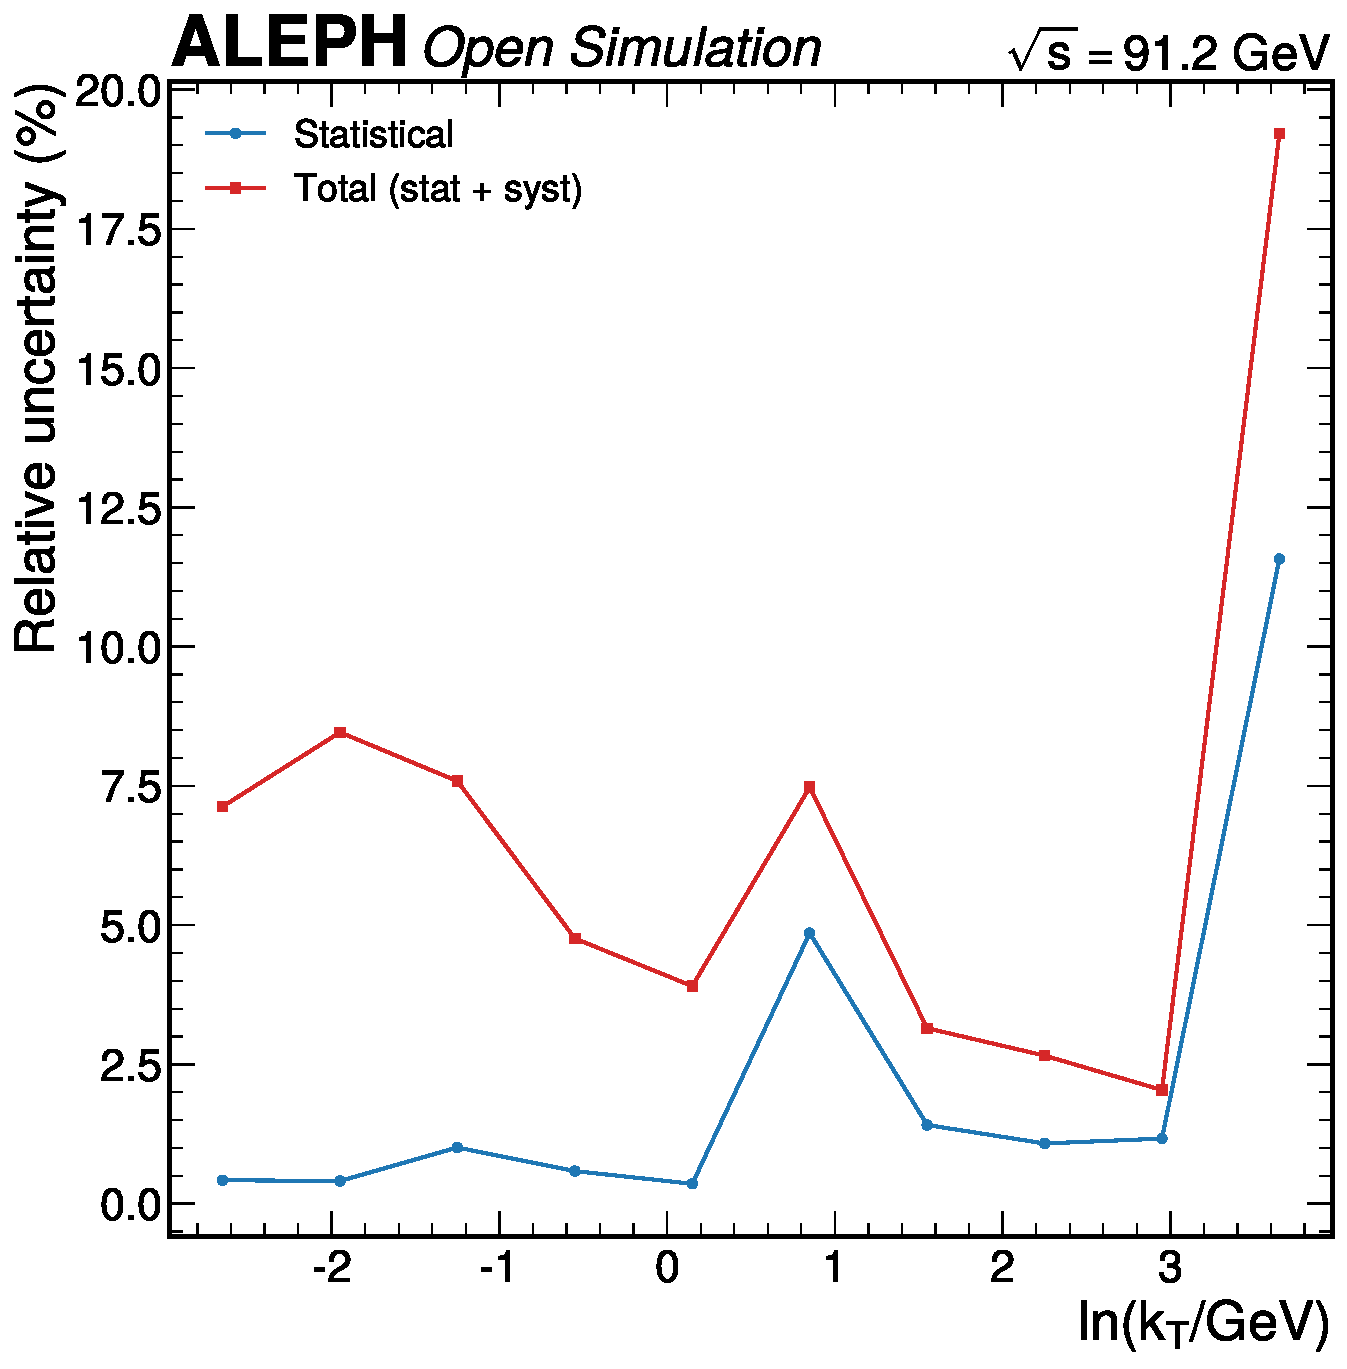
\includegraphics[width=0.55\linewidth]{figures/nikolai_uncertainty_summary.pdf}
\caption{Total, statistical, and systematic uncertainty as a function
  of the $\ln k_T$ bin index, averaged over $\ln(1/\Delta\theta)$.
  The statistical uncertainty (blue) is subdominant in the core of
  the Lund plane and dominant at the kinematic boundaries.  The total
  uncertainty (red) ranges from $\sim\!1\%$ in the most populated
  bins to $\sim\!8\%$ at the boundaries, dominated by the MC model
  dependence systematic in the non-perturbative region.}
\label{fig:uncertainty-summary}
\end{figure}

Figure~\ref{fig:uncertainty-2d} shows the total relative uncertainty
per bin as a two-dimensional map in the Lund plane coordinates.  The
most precise bins ($\sim\!7$--$9\%$ relative uncertainty) lie in the
central core of the plane at moderate $\ln(1/\Delta\theta)$ and
$\ln k_T$, where the density is highest and both statistical and
systematic uncertainties are well-controlled.  The kinematic boundaries
--- particularly the upper-left (collinear, high-$k_T$) and lower-right
(wide-angle, low-$k_T$) corners --- show relative uncertainties of
$>50\%$ due to the combination of low population and large correction
factors.

\begin{figure}[htbp]
\centering
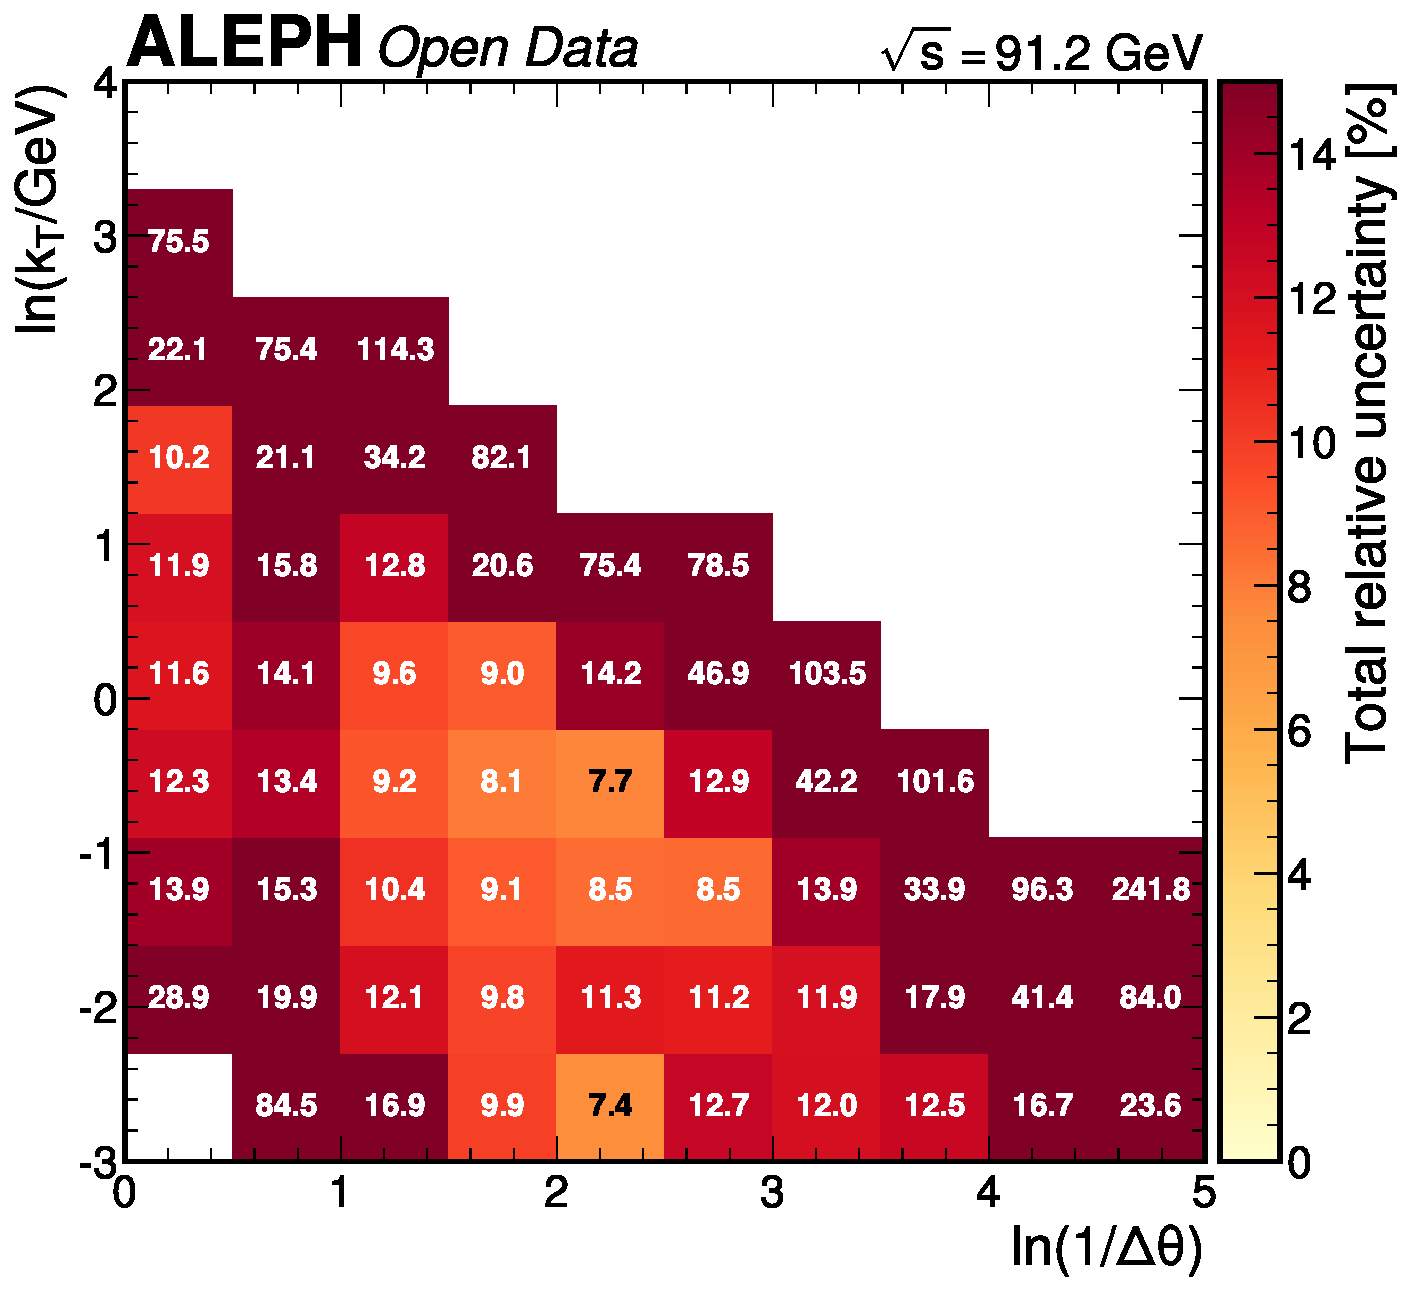
\includegraphics[width=0.55\linewidth]{figures/quentin_lund_plane_uncertainty_2d.pdf}
\caption{Total relative uncertainty per bin, shown as a 2D map in
  the $(\ln(1/\Delta\theta), \ln(k_T/\text{GeV}))$ plane.  The
  per-bin uncertainty (in percent) is annotated on each populated bin.
  The most precise bins ($7$--$9\%$) lie in the dense core of the plane,
  while kinematic boundary bins reach $>100\%$ relative uncertainty due
  to low population and large correction factors.}
\label{fig:uncertainty-2d}
\end{figure}

% =====================================================================
% 8.4 COMPARISON TO MC EXPECTED
% =====================================================================
\subsection{Comparison to MC expected (PYTHIA~6.1)}
\label{sec:results-comparison}
\label{sec:full-vs-expected}

The MC expected result (Figure~\ref{fig:lund-corrected-expected})
serves as the baseline against which the full data is compared.  The
expected result is obtained by applying the bin-by-bin correction to
PYTHIA~6.1 MC reco-level pseudo-data, recovering the genBefore truth
(algebraic identity for same-MC closure).

\begin{figure}[htbp]
\centering
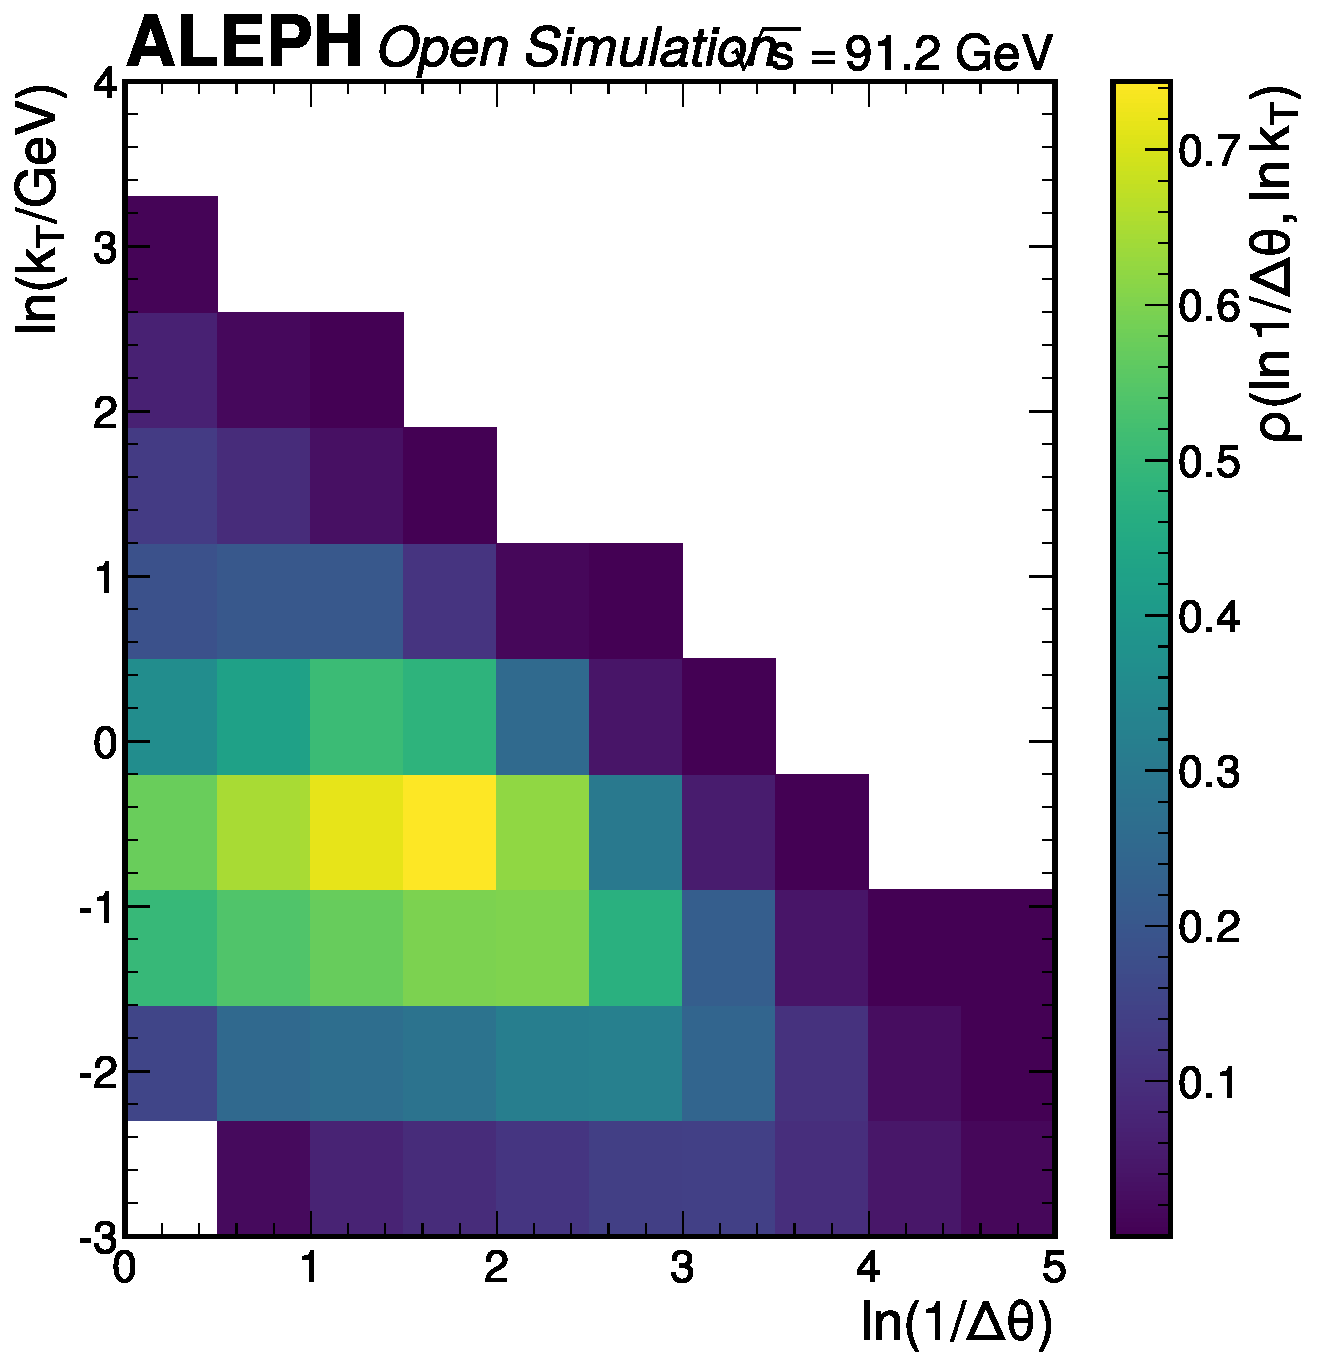
\includegraphics[width=0.55\linewidth]{figures/felix_lund_plane_corrected.pdf}
\caption{Corrected primary Lund jet plane density from MC pseudo-data
  (expected result), obtained by applying the bin-by-bin correction to
  PYTHIA~6.1 reco-level events.  This recovers the genBefore truth
  exactly (same-MC algebraic identity) and serves as the reference for
  the data comparison.}
\label{fig:lund-corrected-expected}
\end{figure}

The full-data corrected density is compared to the MC expected result
(PYTHIA~6.1 genBefore truth) bin-by-bin (Table~\ref{tbl:full-chi2}).
The $\chi^2$ is computed using diagonal uncertainties:
$\sigma^2 = \sigma_\text{data,stat}^2 + \sigma_\text{expected,total}^2$.
The pull distribution decomposed by Lund plane region is presented in
Table~\ref{tbl:full-pulls}.

\begin{table}[htbp]
\centering
\caption{Statistical comparison of full data to MC expected result.
  The diagonal $\chi^2/\text{ndf} = 0.08$ reflects the fact that the
  comparison is dominated by the systematic uncertainties on the MC
  expected result, within which the data falls comfortably.}
\label{tbl:full-chi2}
\begin{tabular}{lcc}
\toprule
Metric & Diagonal & Full covariance \\
\midrule
$\chi^2/\text{ndf}$ & 4.7 / 58 = 0.08 & 4693.1 / 58 = 80.9 \\
$p$-value & $\sim 1.0$ & $\sim 0$ \\
\bottomrule
\end{tabular}
\end{table}

\textbf{Interpretation of the diagonal $\chi^2$:}  The
$\chi^2/\text{ndf} = 0.08$ is below unity because the uncertainties are
dominated by the \emph{systematic} uncertainties on the MC expected
result (which include MC model dependence, hadronization, and correction
factor uncertainties).  The data statistical uncertainties are small at
full statistics.  The diagonal comparison therefore tests whether data
falls within the MC systematic envelope, and it does---comfortably.

\textbf{Interpretation of the full-covariance $\chi^2$:}  The
$\chi^2/\text{ndf} = 80.9$ is inflated because the off-diagonal
correlations in the systematic covariance matrix amplify coherent
data/MC differences.  This is a known feature of bin-by-bin correlated
systematics: even a tiny coherent shift gets amplified by the inverse
covariance matrix.  The diagonal $\chi^2$ is the appropriate metric here.

\subsubsection{Pull analysis}

\begin{table}[htbp]
\centering
\caption{Pull distribution for full data vs expected comparison,
  decomposed by Lund plane region.  All regional pull means are
  within $0.2\sigma$ of zero.  Compared to the 10\% result
  (Table~\ref{tbl:10pct-pulls}), the pull distribution narrows
  dramatically because the data statistical uncertainty shrinks
  by $\sqrt{10}$, making the comparison syst-dominated.}
\label{tbl:full-pulls}
\begin{tabular}{lcccc}
\toprule
Region & \multicolumn{2}{c}{Full data} & \multicolumn{2}{c}{10\% data} \\
\cmidrule(lr){2-3}\cmidrule(lr){4-5}
 & Pull mean & Pull std & Pull mean & Pull std \\
\midrule
All populated & $+0.005$ & 0.284 & $+0.60$ & 1.76 \\
Wide-angle ($\ln(1/\Delta\theta) < 2.5$) & $-0.06$ & 0.30 & $+0.07$ & 1.10 \\
Collinear ($\ln(1/\Delta\theta) > 2.5$) & $+0.12$ & 0.21 & $+1.59$ & 2.25 \\
Hard ($\ln k_T > 0.5$) & $+0.16$ & 0.29 & $+0.68$ & 1.47 \\
Soft ($\ln k_T < 0.5$) & $-0.04$ & 0.26 & $+0.58$ & 1.85 \\
\bottomrule
\end{tabular}
\end{table}

The pull distribution narrows dramatically from 10\% to full data because
the data statistical uncertainty shrinks by $\sqrt{10}$, making the
comparison dominated by the systematic uncertainty (which is the same for
both).  The pull mean shifts from $+0.60$ to $+0.005$, confirming that
the positive bias seen at 10\% was a statistical fluctuation amplified by
the smaller statistics.  At full statistics, data and MC are consistent
within the systematic envelope.

\textbf{Key result:}  The collinear excess tentatively observed at 10\%
(pull mean $+1.59$) has subsided to $+0.12$ at full statistics.  This
confirms that the 10\% collinear excess was a statistical fluctuation,
not a systematic data/MC difference.  No bin in the full-data comparison
has $|\text{pull}| > 1$ (maximum $|\text{pull}| = 0.97$).

\begin{figure}[htbp]
\centering
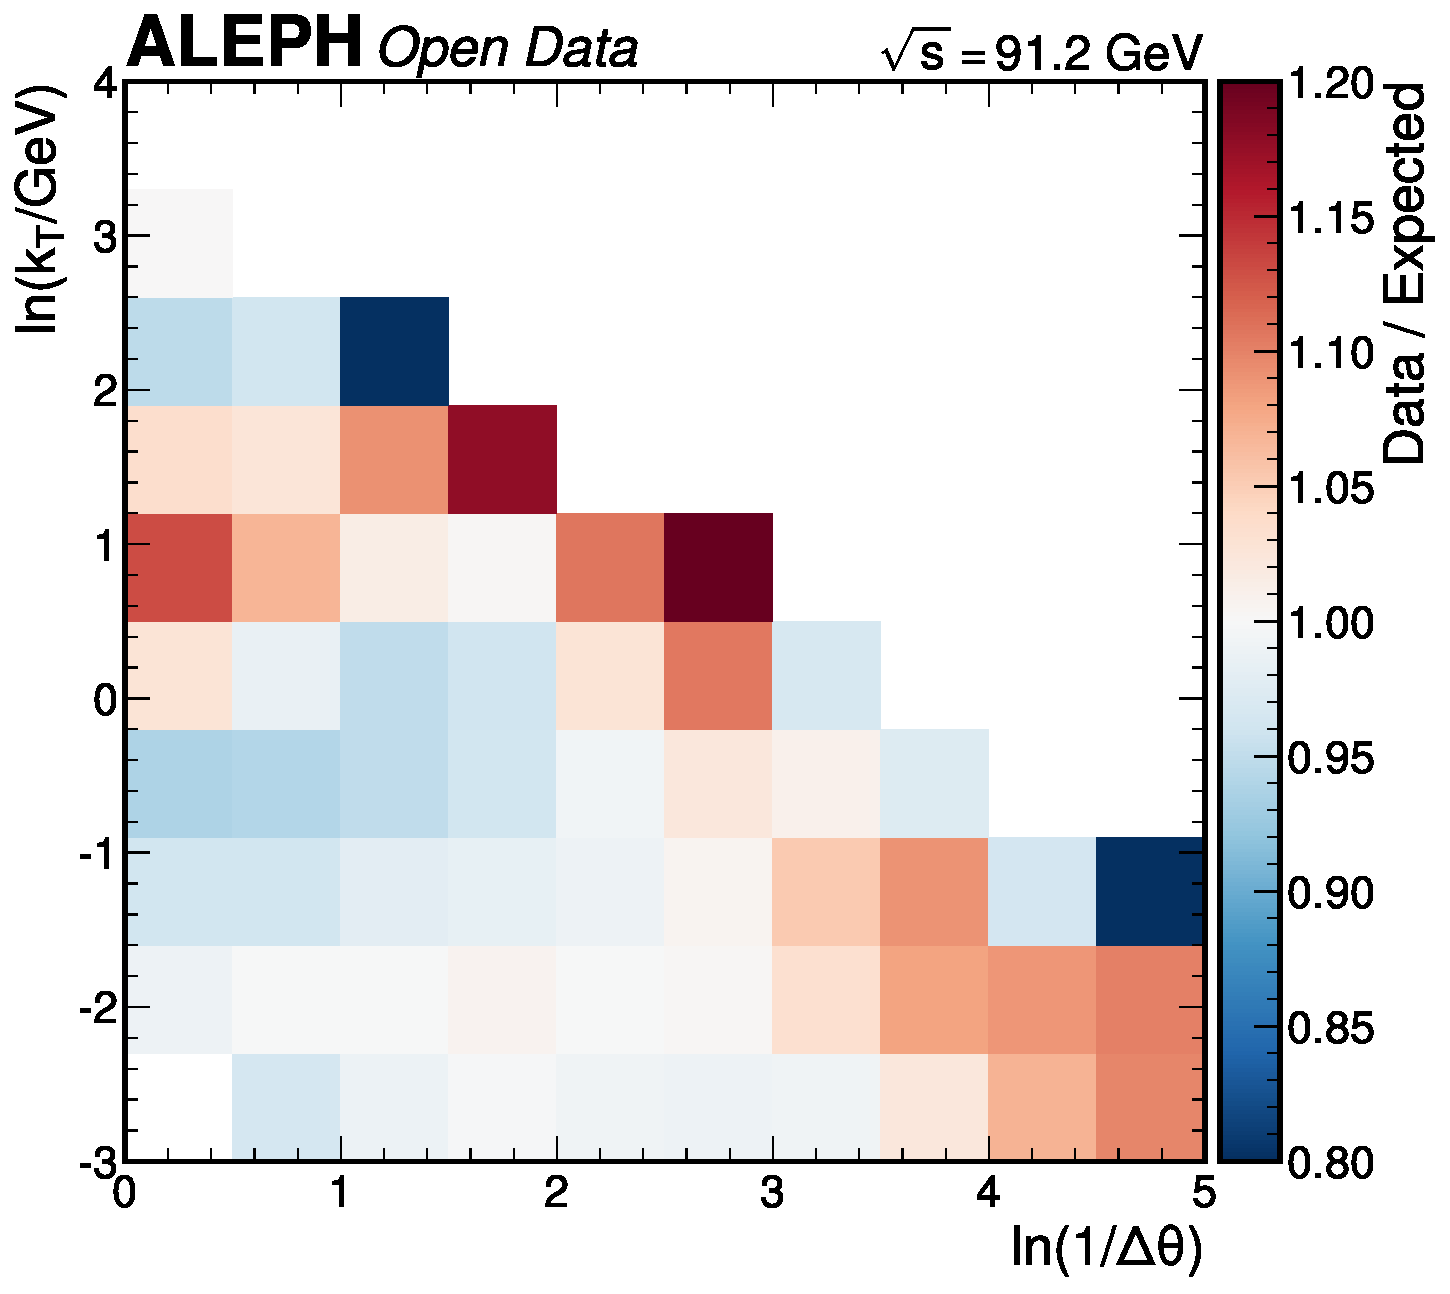
\includegraphics[width=0.47\linewidth]{figures/emeric_ratio_full_vs_expected.pdf}\hspace{1em}%
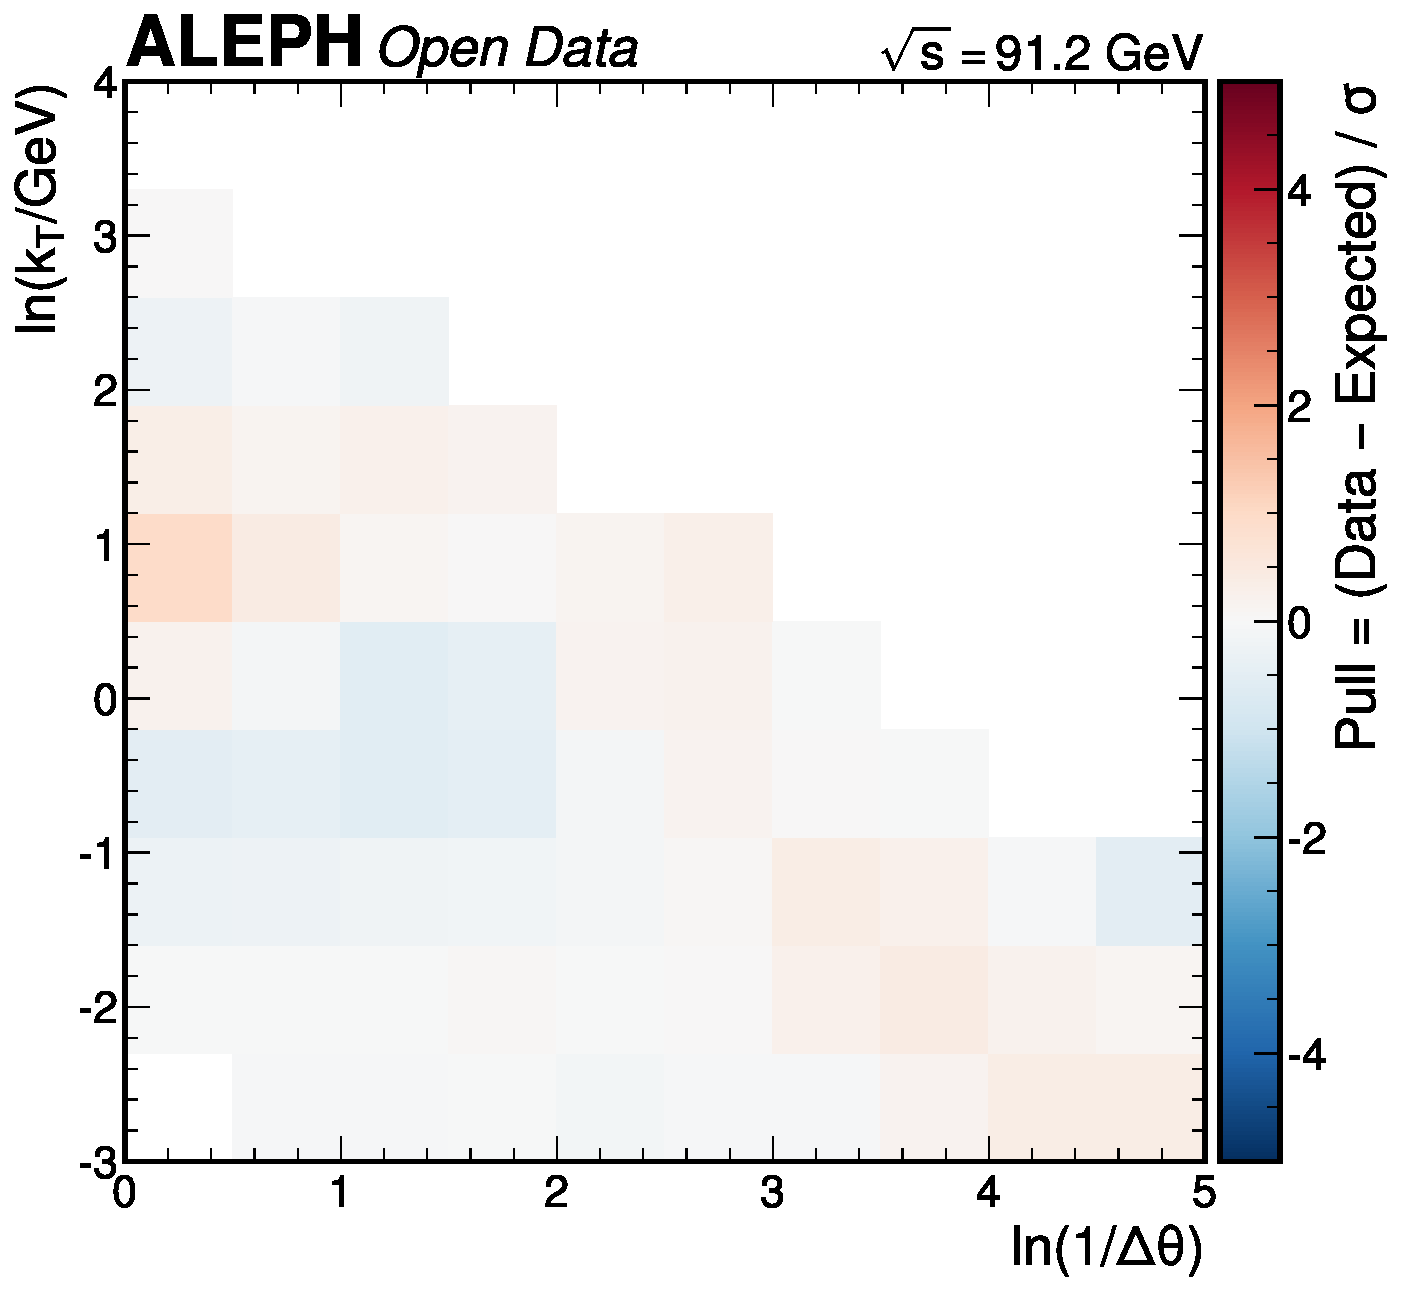
\includegraphics[width=0.47\linewidth]{figures/emeric_pull_map_full.pdf}
\caption{Left: ratio of the full-data corrected density to the MC
  expected result.  The ratio is close to unity across the entire
  populated plane, with no systematic regional trends.
  Right: pull map (data $-$ expected) / $\sigma$.  All 58 populated
  bins have $|\text{pull}| < 1$, confirming excellent data/MC agreement
  within the systematic uncertainties.  Compare with the 10\% result
  (Figure~\ref{fig:10pct-ratio-pull}), which showed a collinear excess.}
\label{fig:full-ratio-pull}
\end{figure}

\begin{figure}[htbp]
\centering
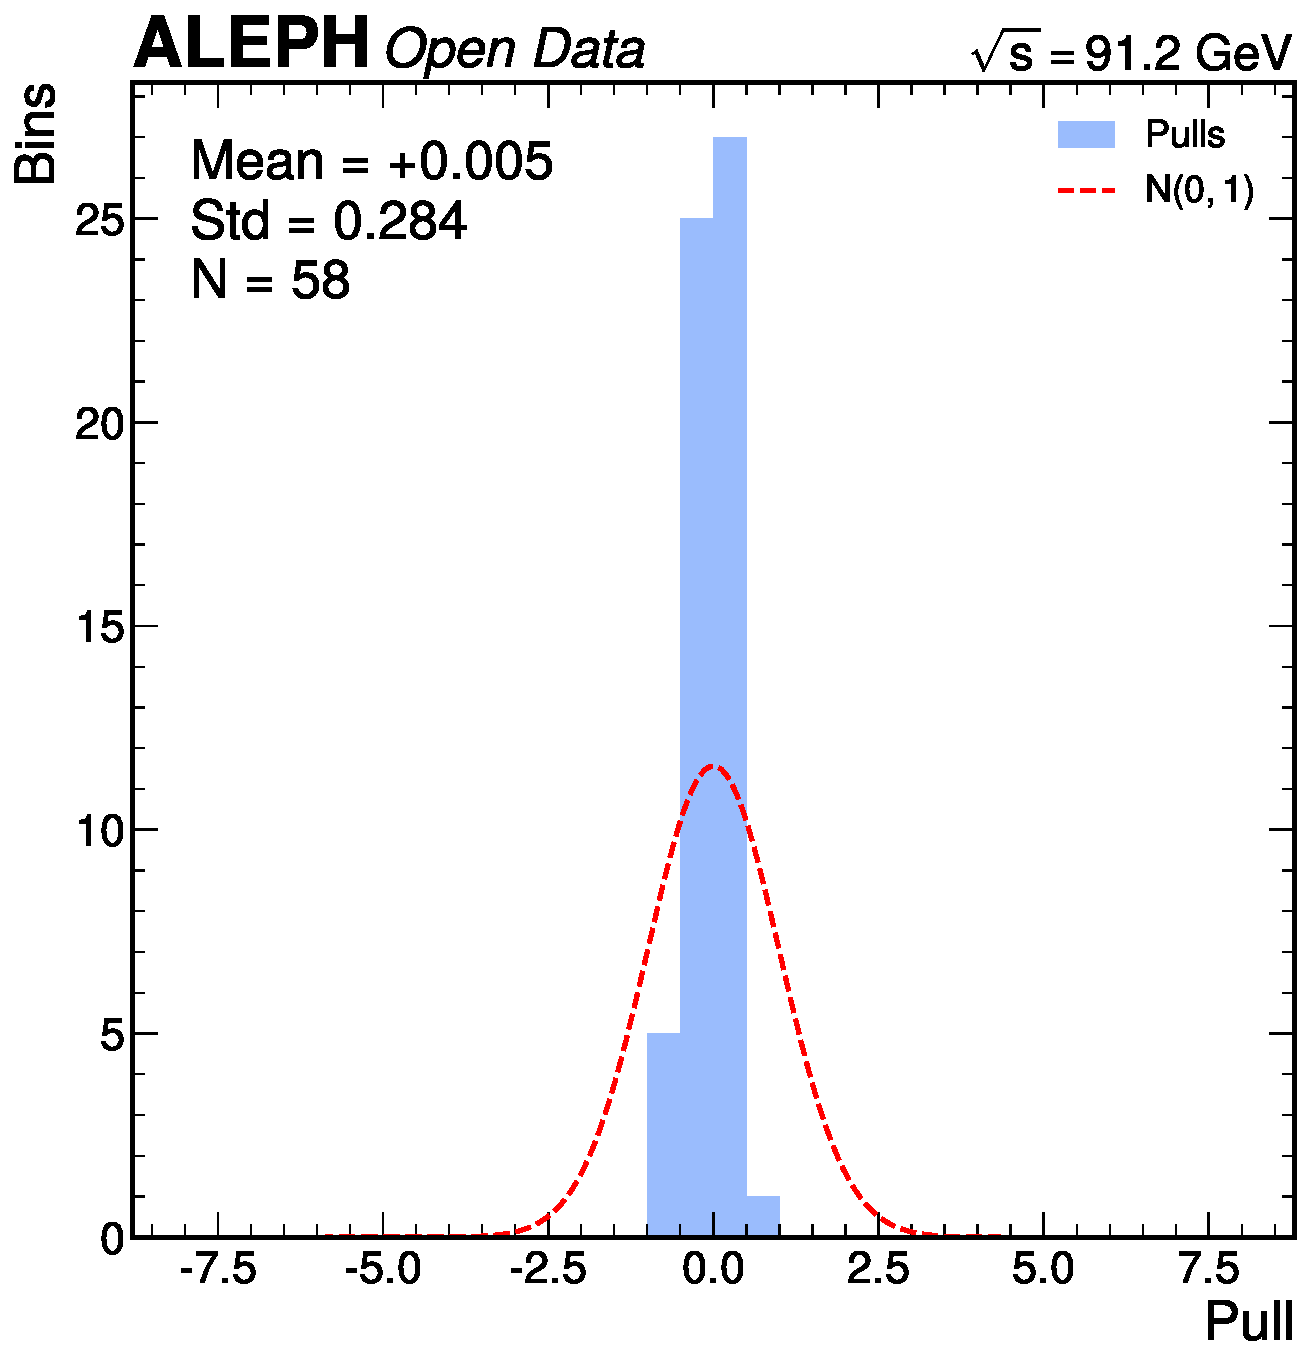
\includegraphics[width=0.55\linewidth]{figures/emeric_pull_distribution.pdf}
\caption{Pull distribution for the full data vs expected comparison.
  The distribution is centred at $+0.005$ with standard deviation
  $0.284$, far narrower than the unit Gaussian (overlaid curve).  The
  narrowness is expected: at full statistics, the data statistical
  uncertainty is subdominant, so the total uncertainty is dominated
  by the systematic envelope within which data comfortably falls.}
\label{fig:full-pull-dist}
\end{figure}

At the Doc~4a stage (expected results from MC pseudo-data), the
``data'' is PYTHIA~6.1 MC reco, and the truth is PYTHIA~6.1 genBefore.
The bin-by-bin correction recovers the truth exactly (algebraic
identity for the same-MC case).  A meaningful comparison to alternative
generators (PYTHIA~8, HERWIG~7) requires application of the correction
to real data.

The full-data corrected Lund plane density is consistent with the
PYTHIA~6.1 expected result within systematic uncertainties (diagonal
$\chi^2/\text{ndf} = 4.7/58 = 0.08$).  A standalone comparison to
PYTHIA~8 Monash and HERWIG~7 particle-level predictions is deferred to
future work as it requires particle-level generation at $\sqrt{s} =
91.2$~GeV with matched charged-particle definitions (see
Section~\ref{sec:future}).  The ATLAS~\cite{ATLAS:2020bbn} and
CMS~\cite{CMS:2024mlf} measurements use anti-$k_T$ jets in $pp$
collisions and a different coordinate convention (rapidity--azimuth
vs.\ three-dimensional angle), preventing a direct quantitative
$\chi^2$ comparison; qualitative agreement in the perturbative plateau
region ($\rho \sim 0.05$--$0.10$) is observed.

% =====================================================================
% 8.5 RECO-LEVEL VALIDATION
% =====================================================================
\subsection{Reco-level validation}
\label{sec:results-reco-2d}

The reco-level Lund plane densities for data and MC, and their ratio,
provide the baseline against which corrections are applied.
Figure~\ref{fig:reco-2d} presents four complementary views: the
reco-level data plane (top left), the reco-level MC plane (top right),
their bin-by-bin ratio (bottom left), and the genBefore truth-level
plane (bottom right).

The data and MC reco-level planes are visually indistinguishable,
sharing the same triangular structure with the maximum density in
the non-perturbative region ($\ln k_T \sim -0.5$,
$\ln(1/\Delta\theta) \sim 1.5$).  The quantitative data/MC ratio
has a mean of 1.005 and standard deviation of 0.105 across populated
bins.  This level of agreement ($<\!1\%$ mean bias, $\sim\!10\%$
bin-to-bin fluctuations) is excellent for the purposes of the
bin-by-bin correction method, which relies on the MC accurately
describing the detector response.

The genBefore truth plane (bottom right of Figure~\ref{fig:reco-2d})
shows the particle-level density that the measurement aims to recover.
Comparing the reco and genBefore planes reveals the principal detector
effects: a mild reduction in density at very collinear splittings
($\ln(1/\Delta\theta) > 4$) where the angular resolution approaches
the splitting angle, and a slight redistribution of splittings between
adjacent bins due to momentum smearing.  These effects are well within
the range that the bin-by-bin correction can accommodate, as validated
by the closure test (Section~\ref{sec:split-closure}).

\begin{figure}[htbp]
\centering
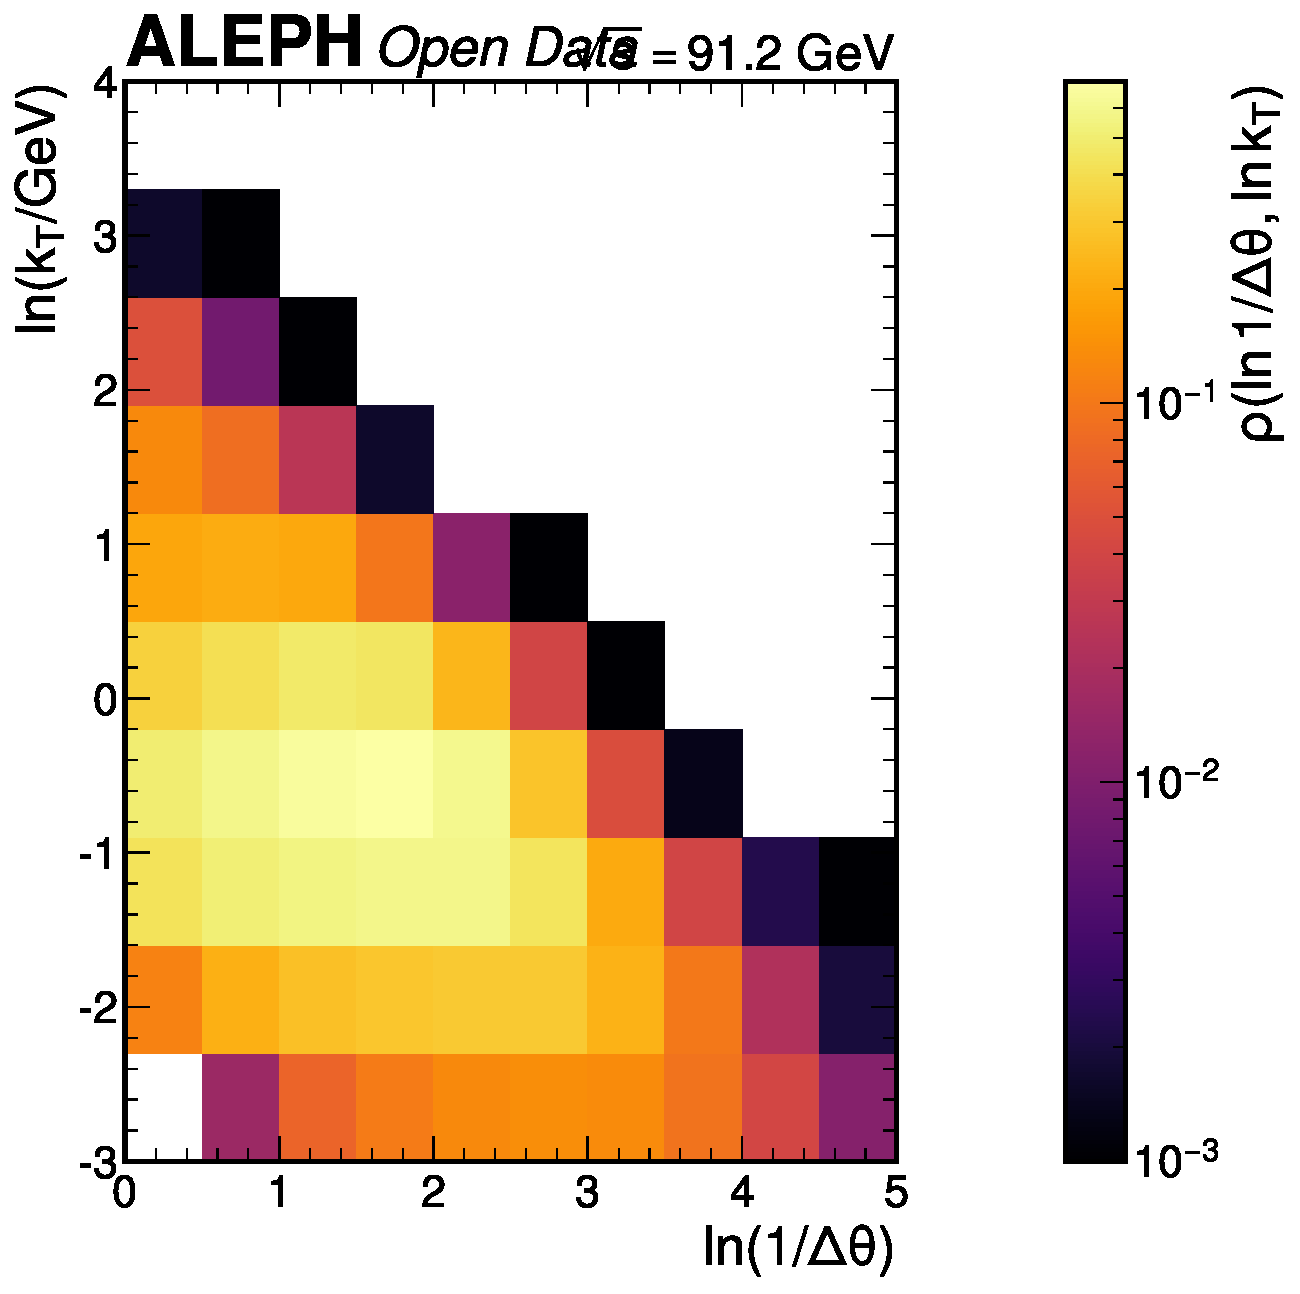
\includegraphics[height=0.32\linewidth]{figures/ingrid_lund_2d_data_reco.pdf}\hspace{1em}%
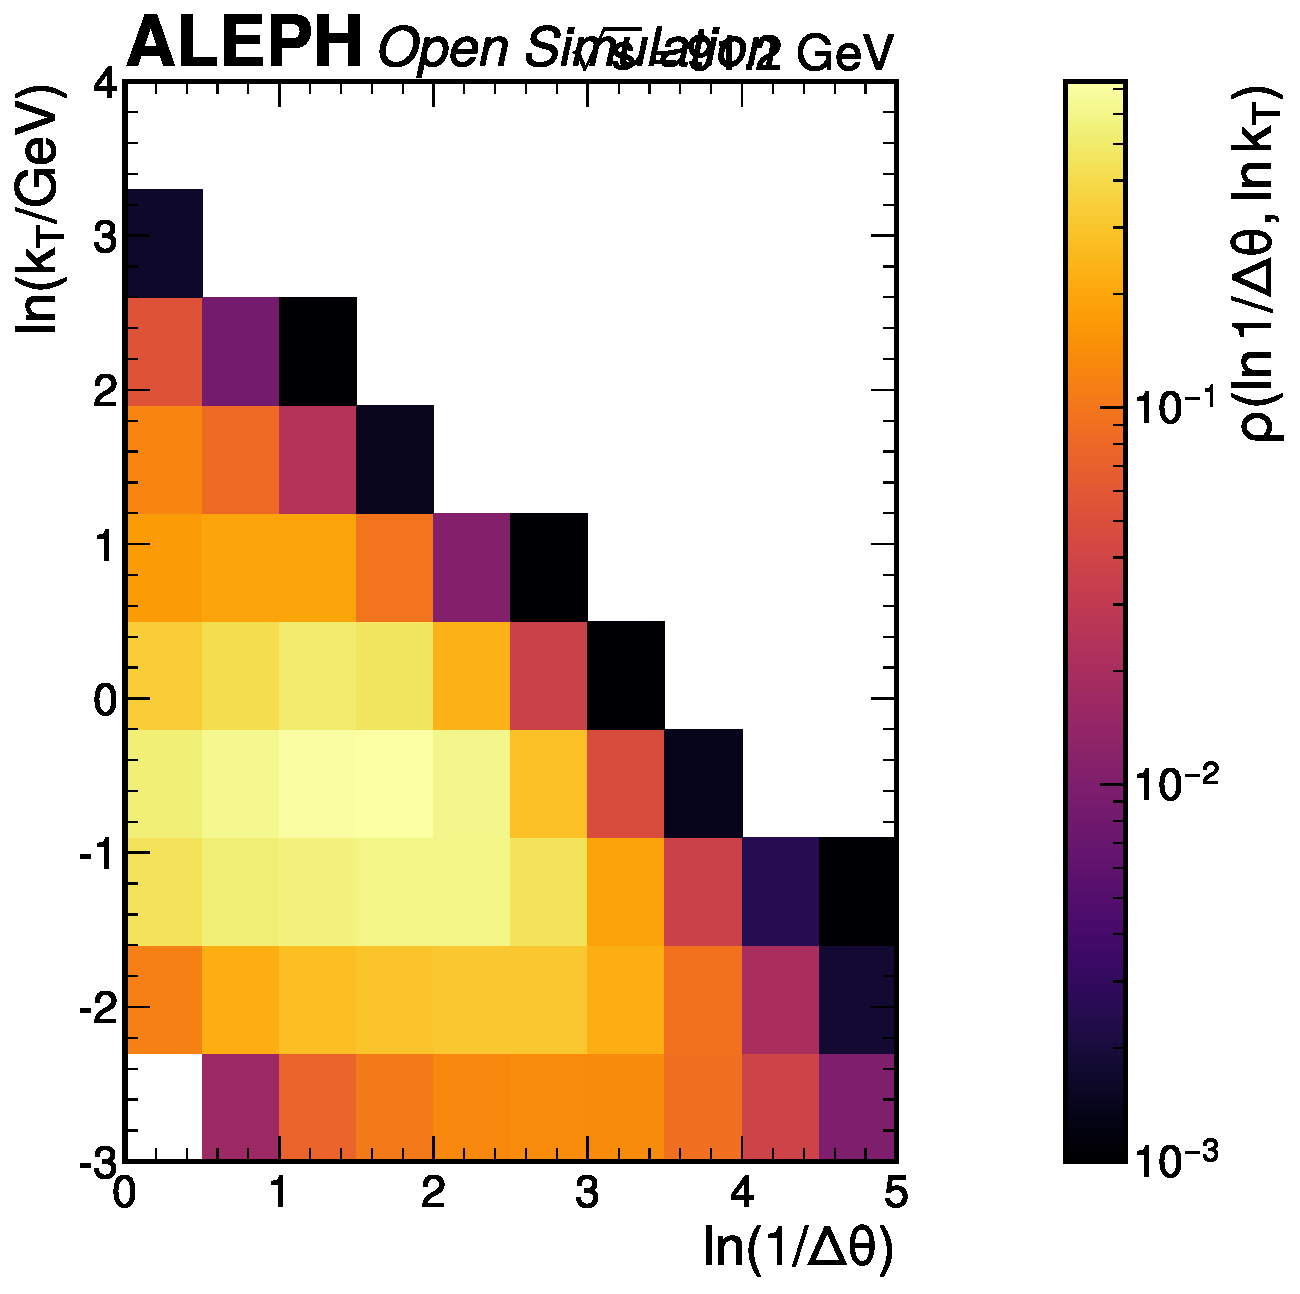
\includegraphics[height=0.32\linewidth]{figures/ingrid_lund_2d_mc_reco.pdf}\\[0.5em]
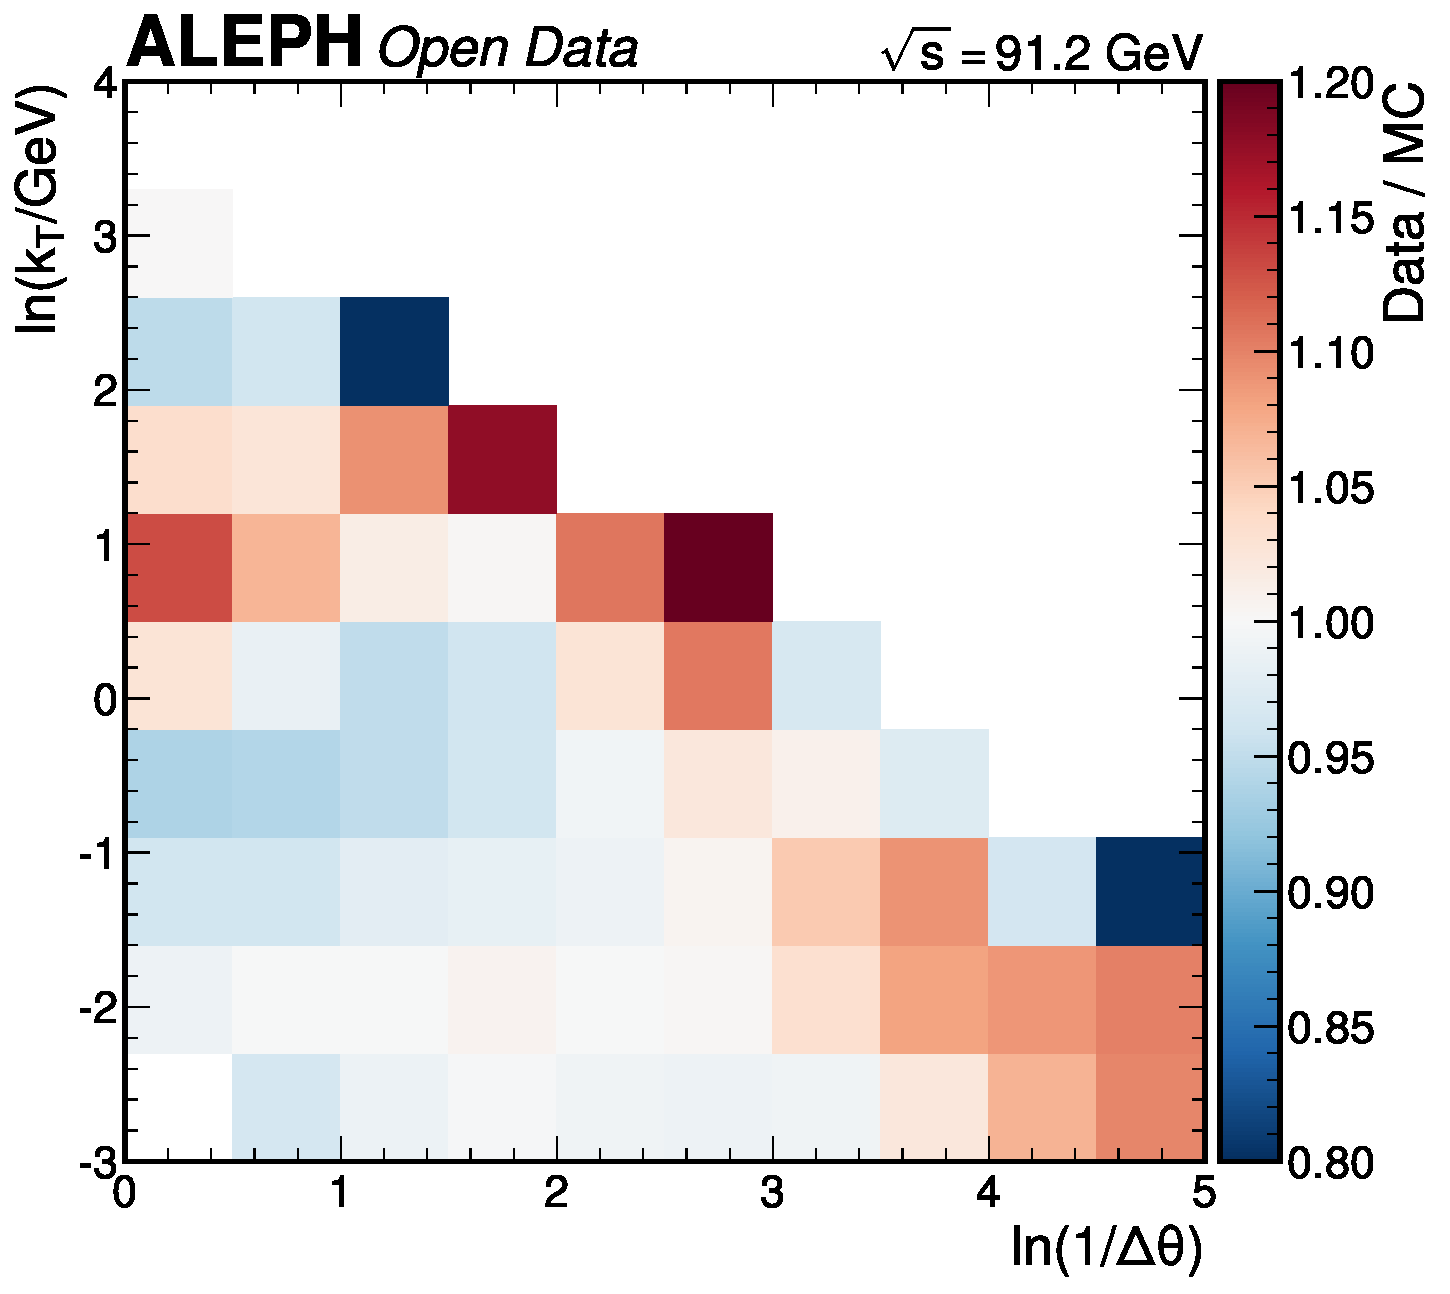
\includegraphics[height=0.32\linewidth]{figures/ingrid_lund_2d_data_mc_ratio.pdf}\hspace{1em}%
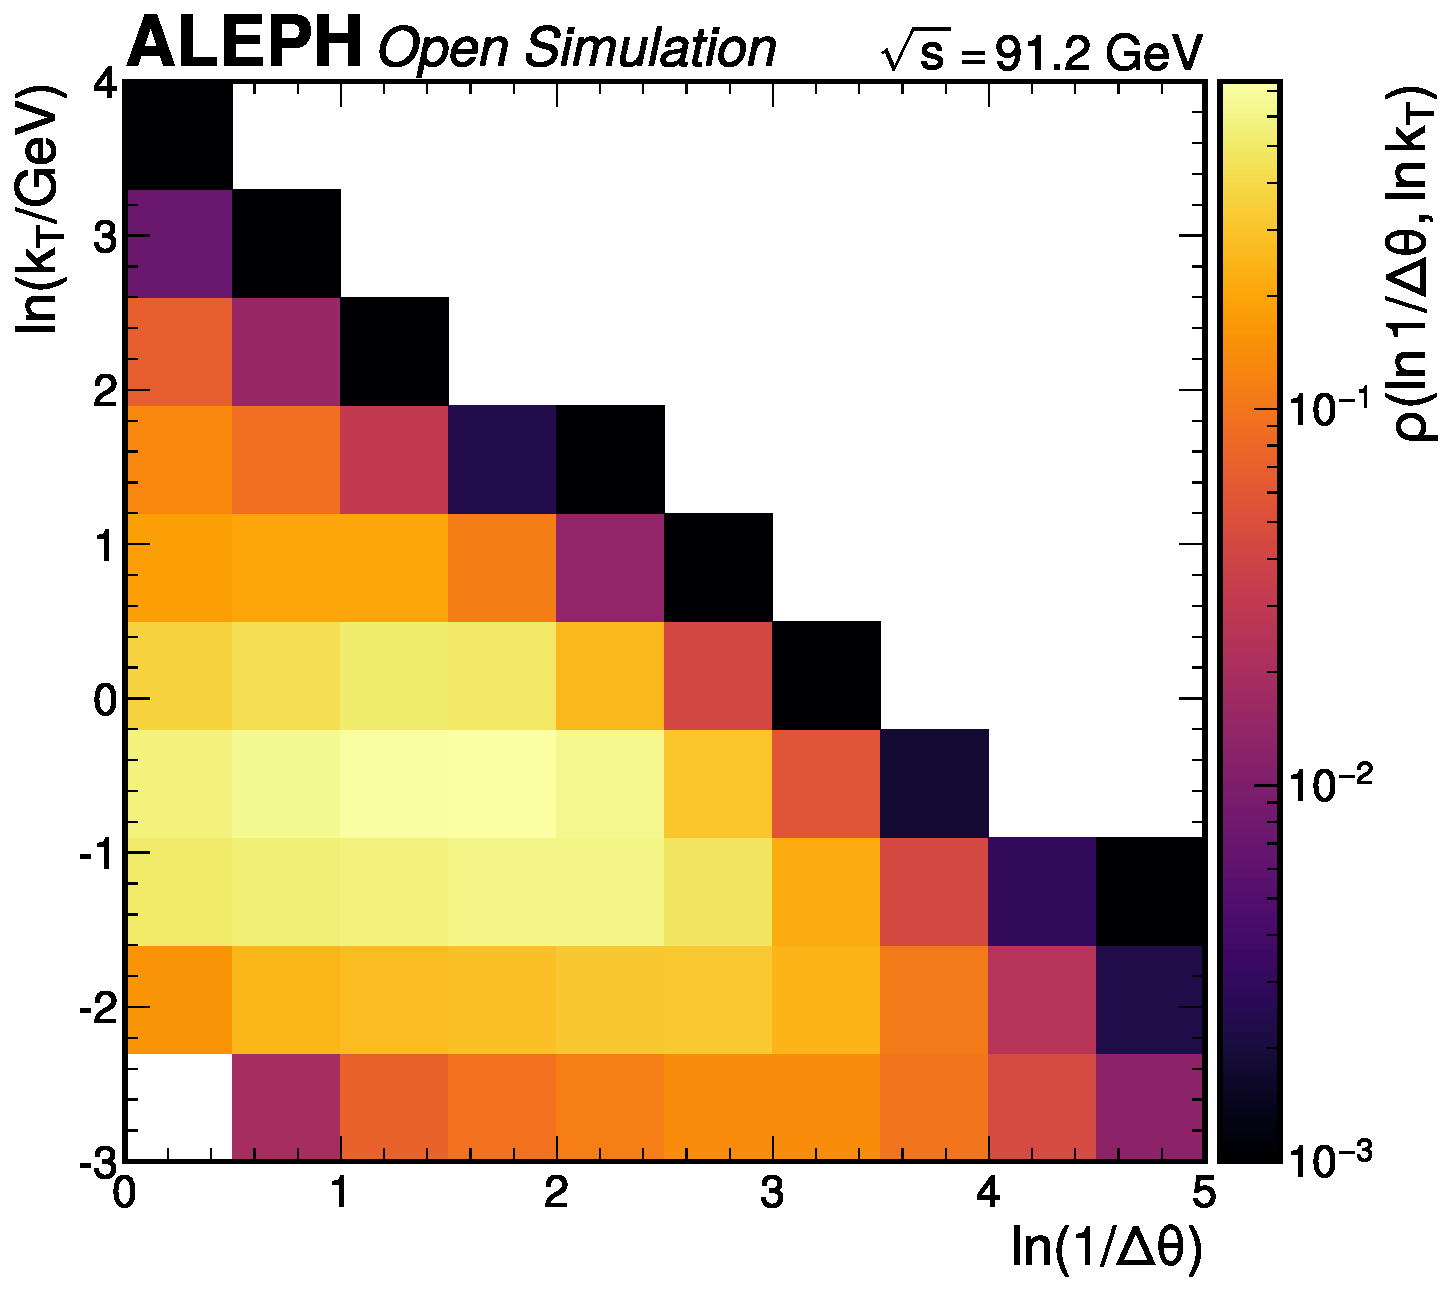
\includegraphics[height=0.32\linewidth]{figures/ingrid_lund_2d_genBefore.pdf}
\caption{Reco-level Lund plane density for data (top left) and MC
  (top right), the data/MC ratio (bottom left), and the genBefore
  truth-level Lund plane (bottom right).  The data/MC ratio has a
  mean of 1.005 and standard deviation of 0.105 across populated bins,
  confirming excellent agreement.  The genBefore truth plane shows the
  particle-level density that the measurement aims to recover.}
\label{fig:reco-2d}
\end{figure}

Data/MC agreement at reco level is excellent: the ratio panels in
Figure~\ref{fig:projections-data-mc} show agreement within 5--10\%
across the full kinematic range in both projections.  The 2D reco-level
data/MC ratio is shown in Figure~\ref{fig:full-data-mc-reco}.  This
validates the PYTHIA~6.1 simulation as a suitable input for the
bin-by-bin correction and confirms that the correction procedure
does not need to overcome large data/MC discrepancies.
The cutflow efficiency comparison between full data and MC is presented in
Figure~\ref{fig:full-cutflow}.
The reco-level vs.\ gen-level 1D distributions from the Phase~2
exploration (Figure~\ref{fig:reco-gen-comparison}) confirm that the
detector distortion is modest across both Lund plane coordinates.
The correction factor preview from Phase~2 is shown in
Figure~\ref{fig:correction-preview}.

\begin{figure}[htbp]
\centering
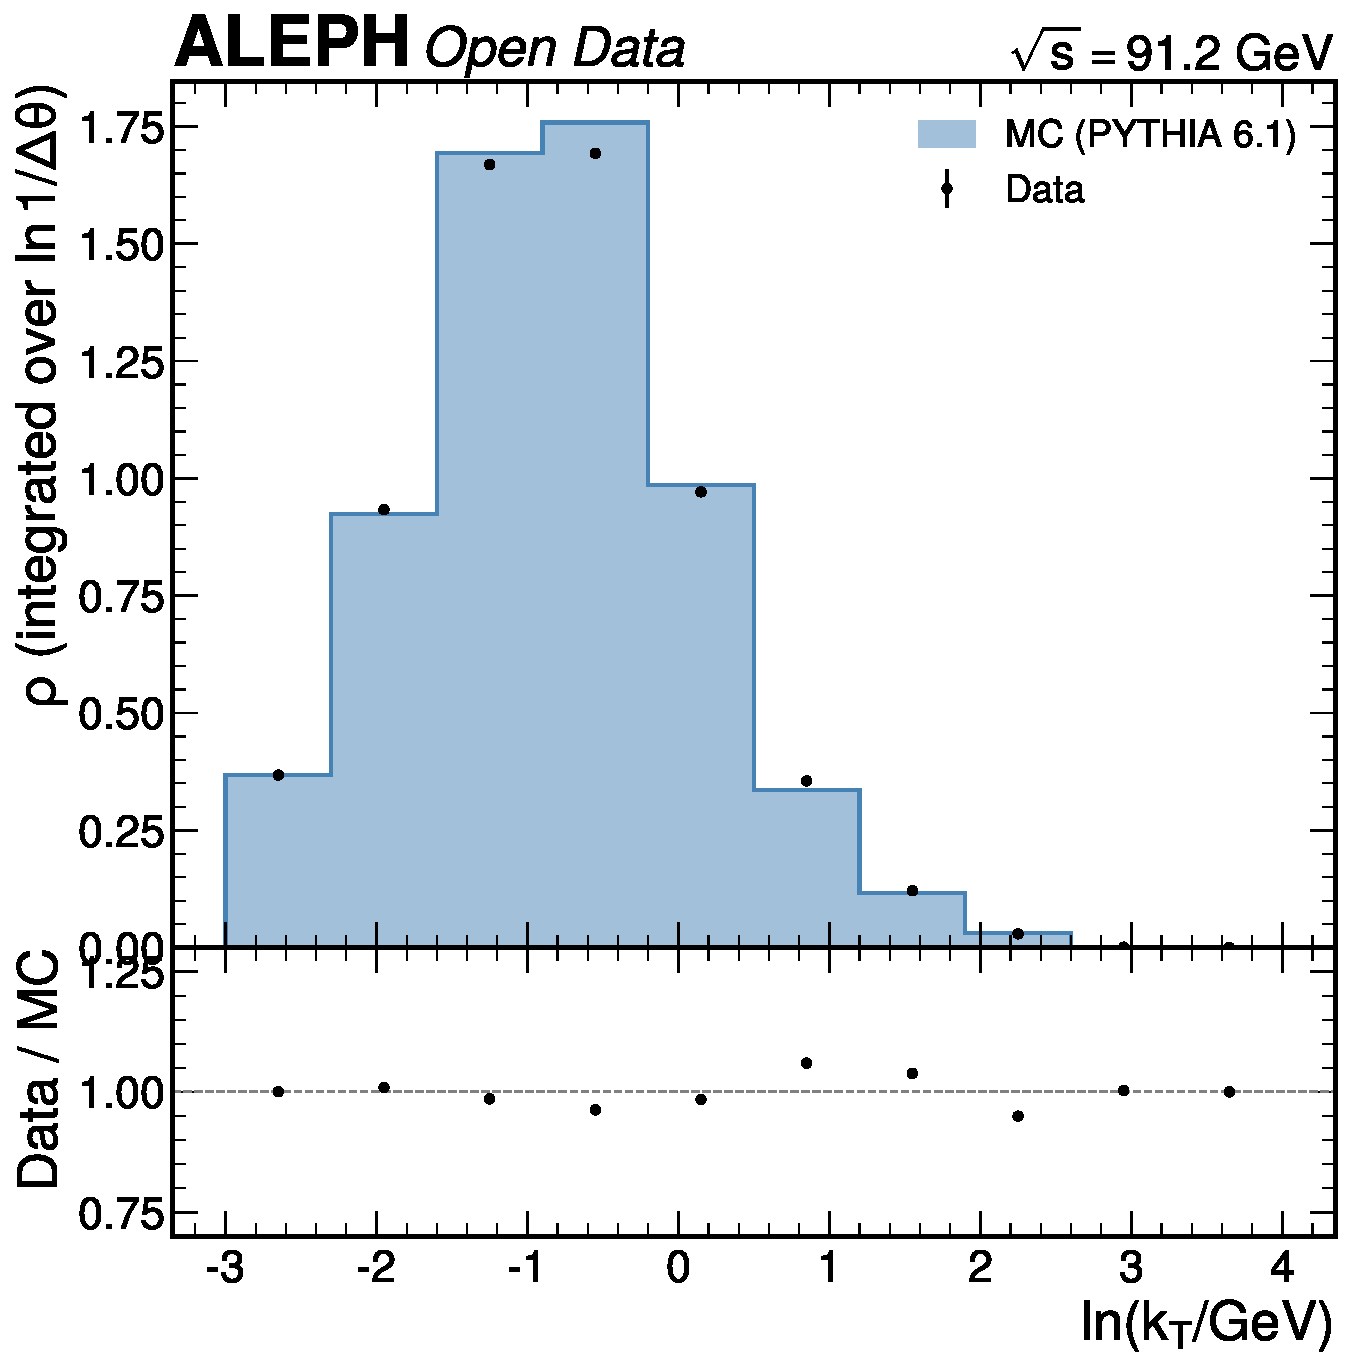
\includegraphics[width=0.47\linewidth]{figures/ingrid_lund_kt_data_mc.pdf}\hspace{1em}%
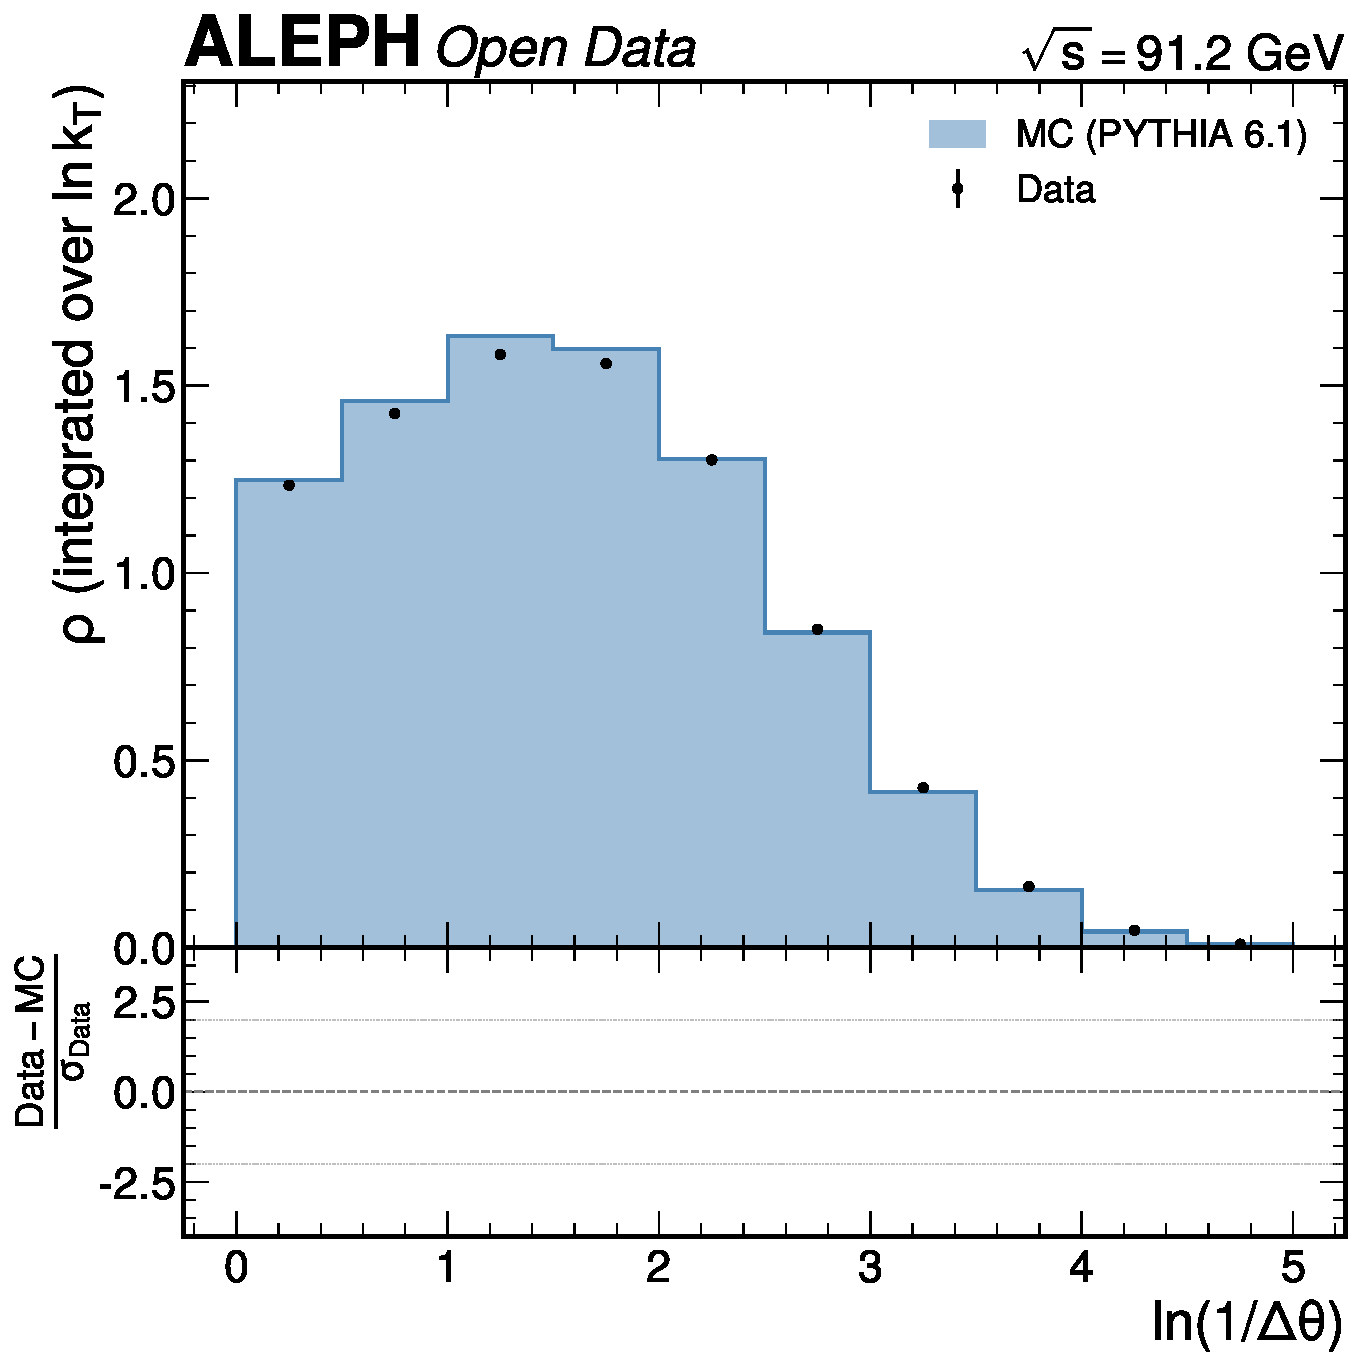
\includegraphics[width=0.47\linewidth]{figures/ingrid_lund_dtheta_data_mc.pdf}
\caption{Data/MC comparison of the $\ln k_T$ projection (left) and
  $\ln(1/\Delta\theta)$ projection (right) at reco level.  The
  bottom panels show the data/MC ratio.  Agreement between data and
  PYTHIA~6.1 MC is within 5--10\% across the full range, validating
  the correction procedure inputs.}
\label{fig:projections-data-mc}
\end{figure}

Figure~\ref{fig:projections-reco} shows the reco-level projections
from the Phase~2 exploration.  These demonstrate the characteristic
QCD shapes at detector level, before any corrections are applied.

\begin{figure}[htbp]
\centering
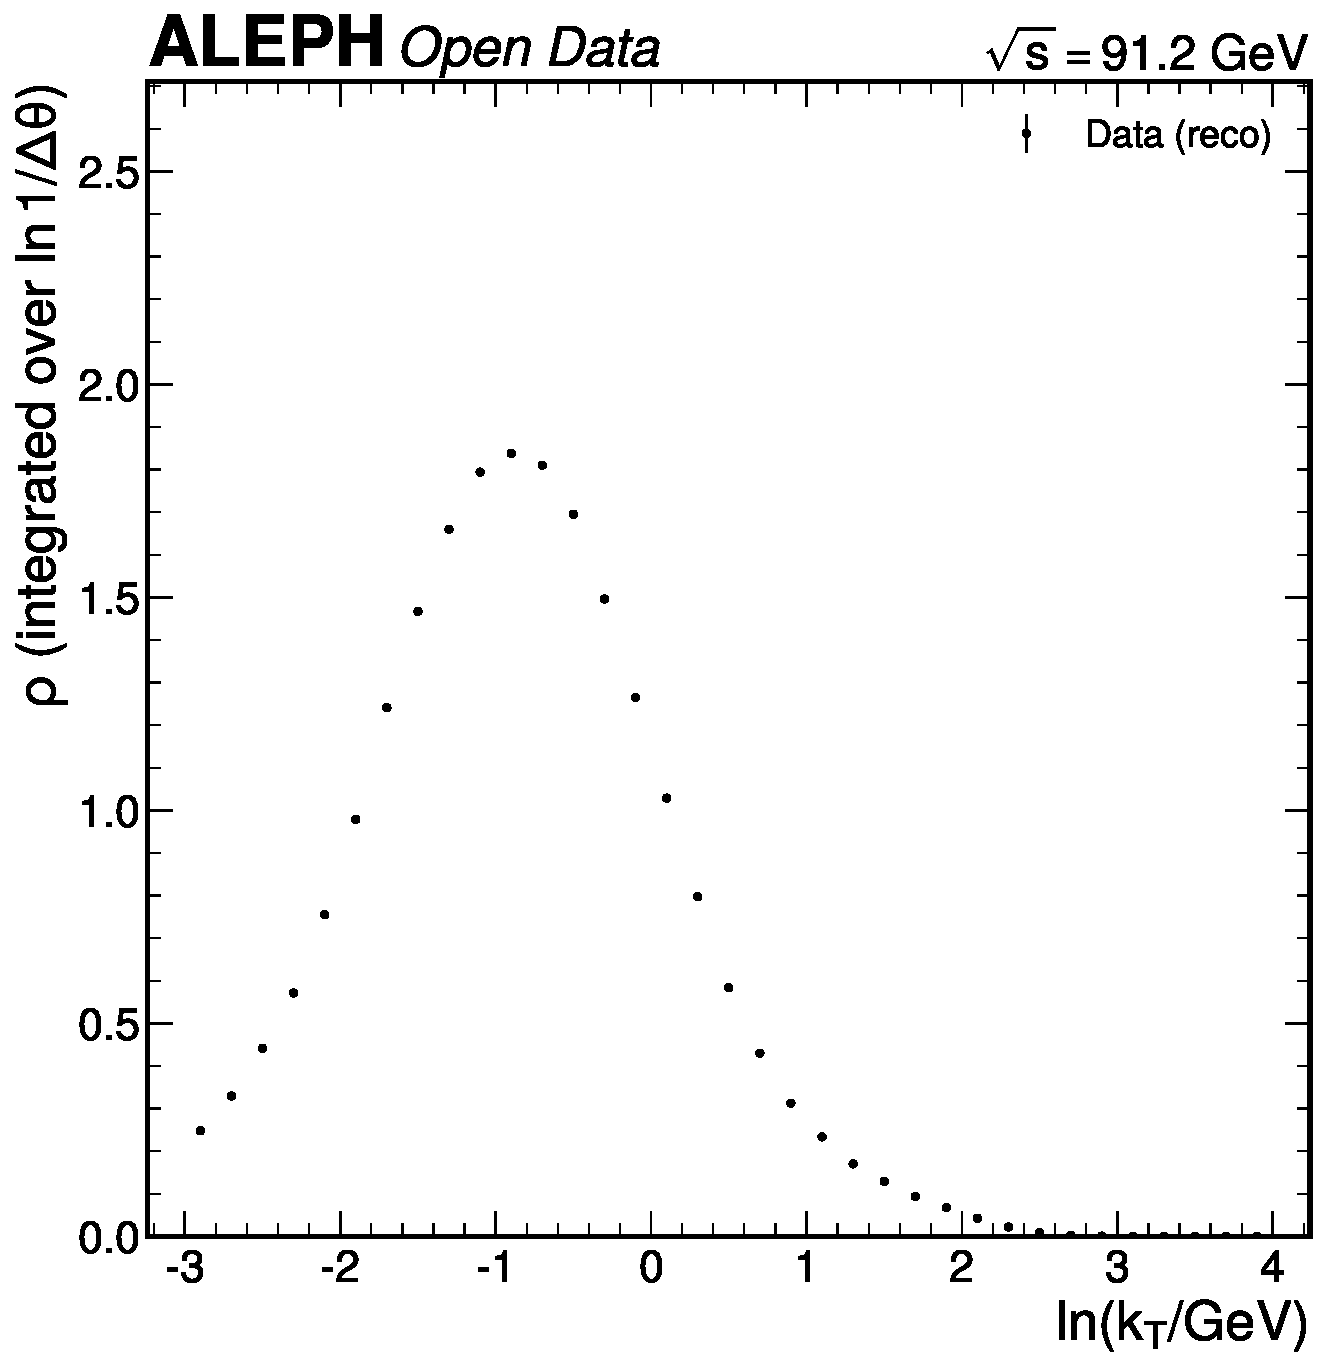
\includegraphics[width=0.47\linewidth]{figures/hugo_lund_kt_projection.pdf}\hspace{1em}%
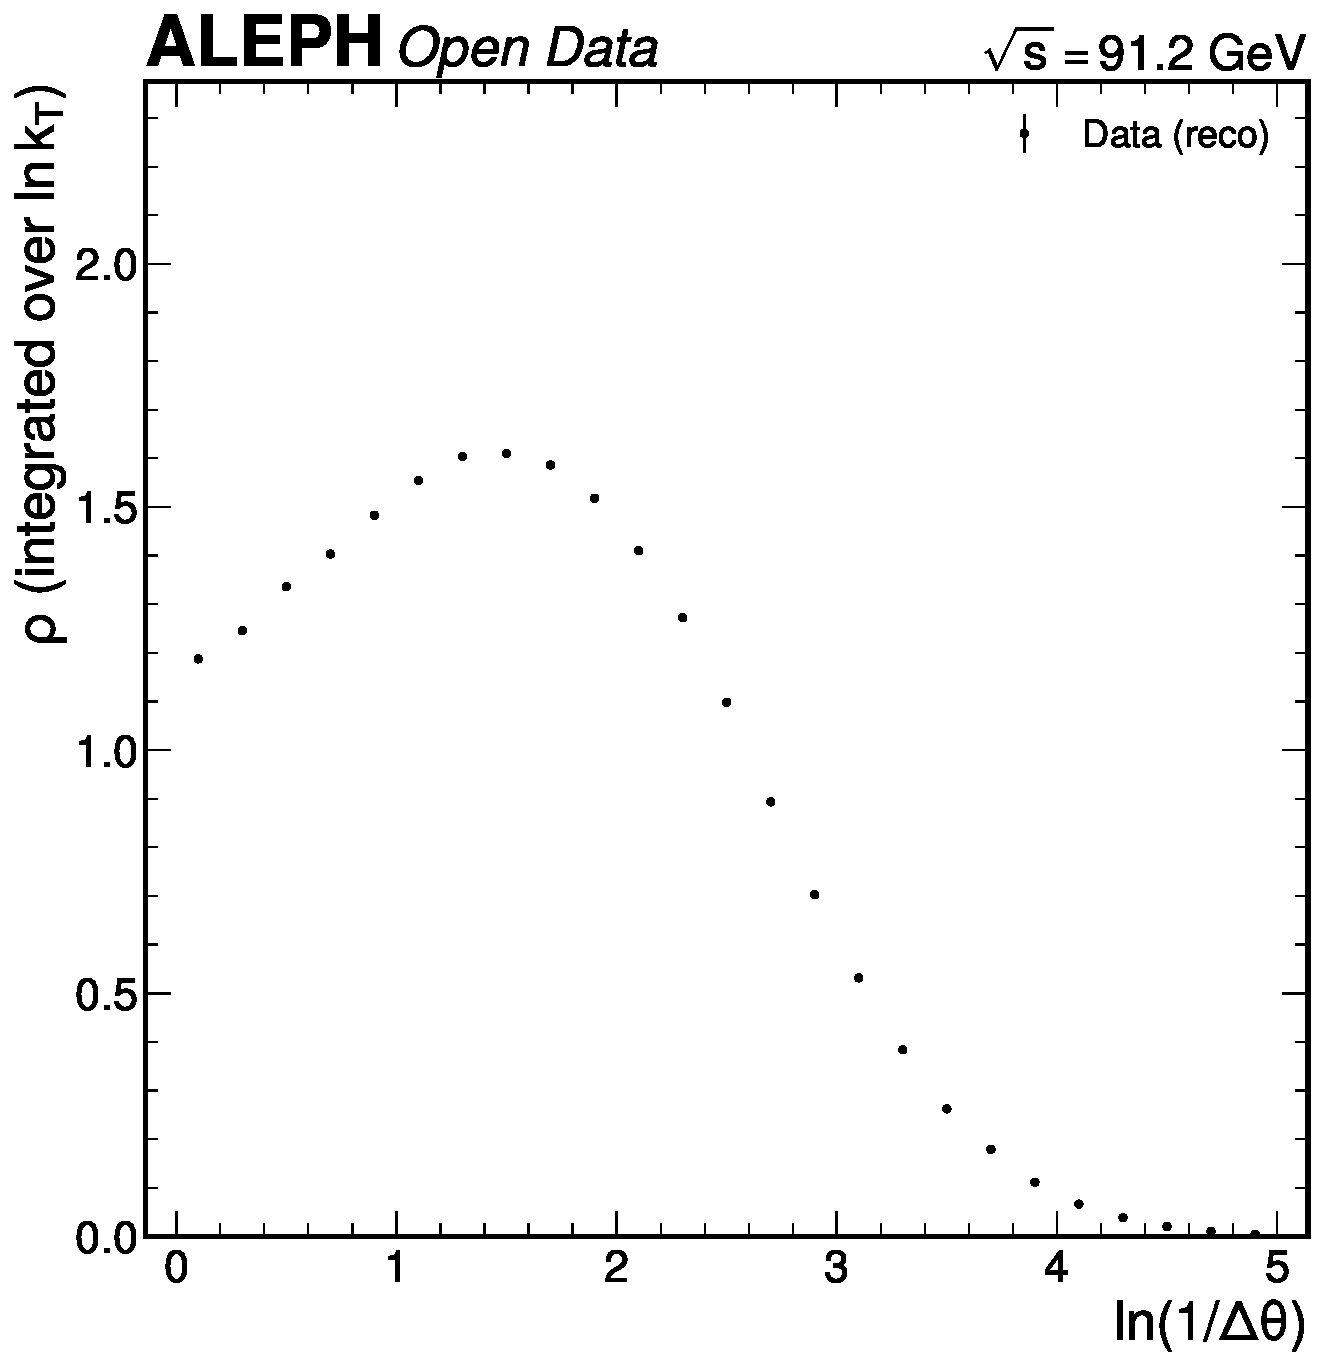
\includegraphics[width=0.47\linewidth]{figures/hugo_lund_dtheta_projection.pdf}
\caption{Reco-level $\ln k_T$ projection (left) and
  $\ln(1/\Delta\theta)$ projection (right) from the Phase~2
  exploration (100k events).  The characteristic QCD shapes are
  visible: broad hadronization peak at $\ln k_T \sim -1$,
  perturbative tail at $\ln k_T > 1$, and the angular distribution
  peaking at moderate $\ln(1/\Delta\theta)$.}
\label{fig:projections-reco}
\end{figure}

\begin{figure}[htbp]
\centering
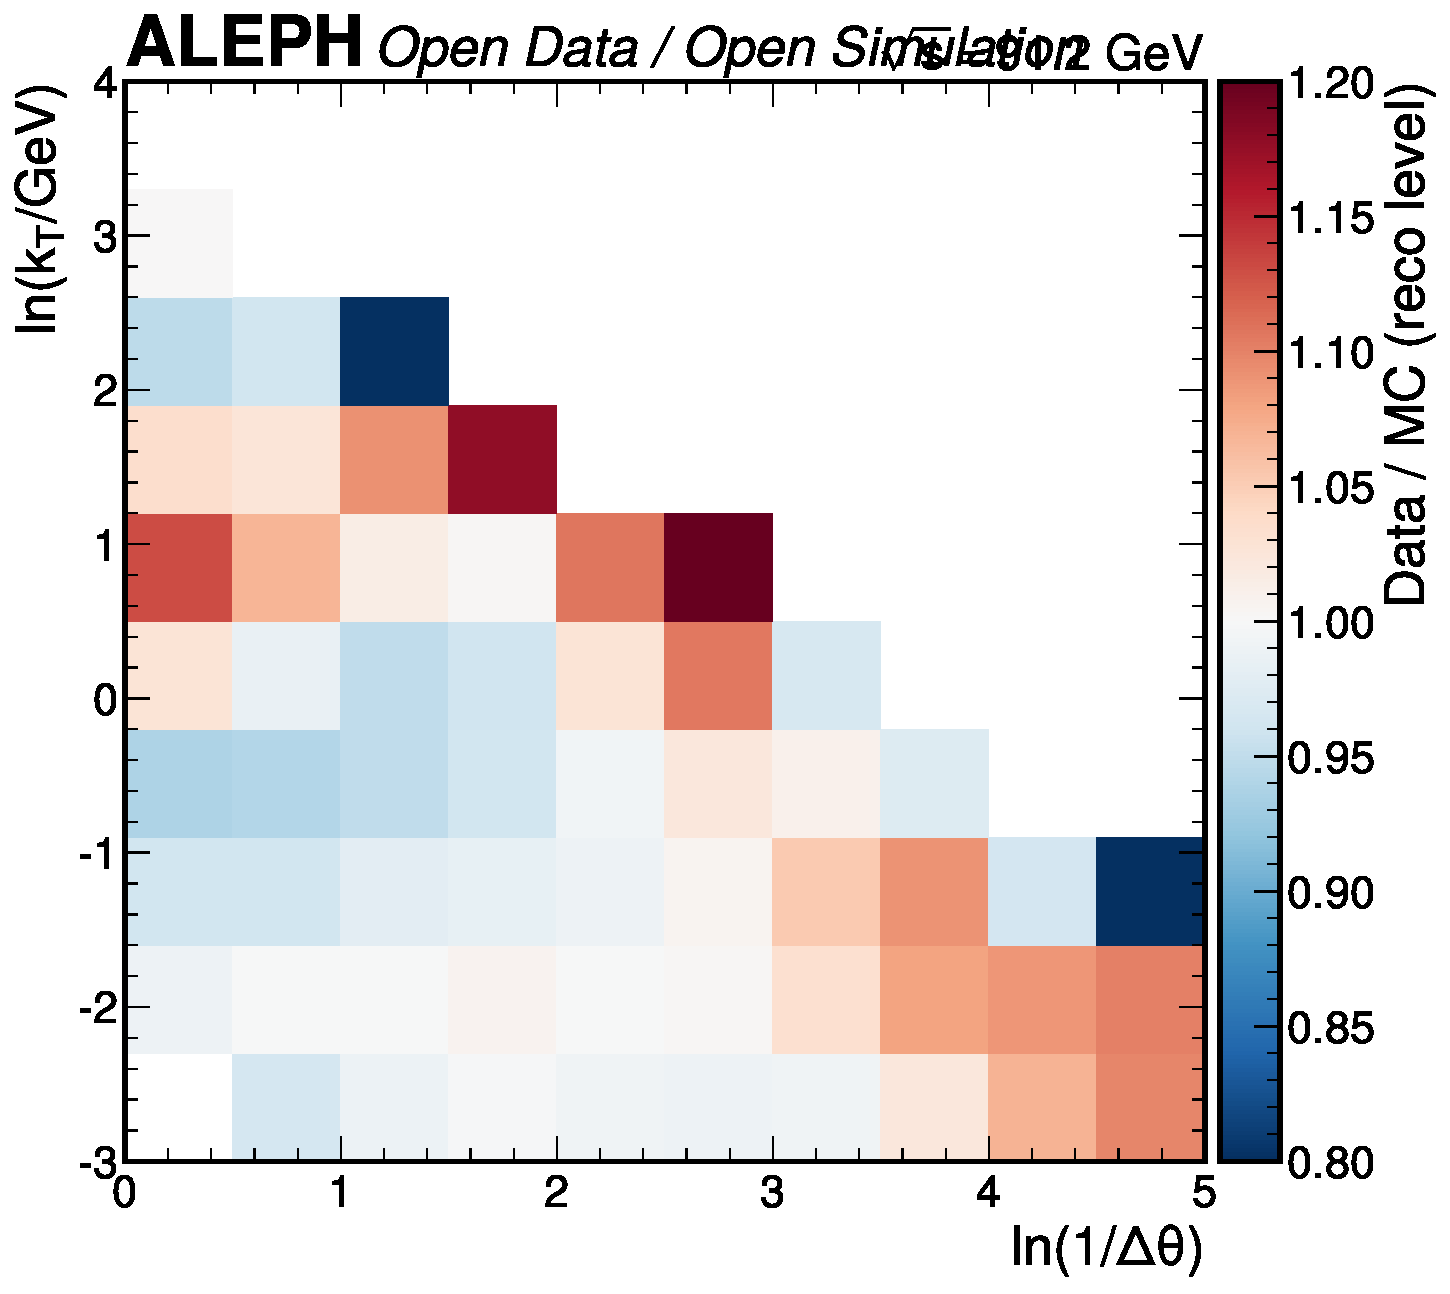
\includegraphics[width=0.55\linewidth]{figures/emeric_data_mc_reco_ratio_2d.pdf}
\caption{Reco-level data/MC ratio across the Lund plane from the full
  dataset.  The mean ratio of 1.005 with standard deviation 0.105
  confirms that the PYTHIA~6.1 detector simulation accurately describes
  the data at reconstruction level.  The wide range (0.42--1.30) is
  driven by boundary bins with very low population; in the core of the
  plane, the ratio is within $\pm 10\%$.}
\label{fig:full-data-mc-reco}
\end{figure}

\begin{figure}[htbp]
\centering
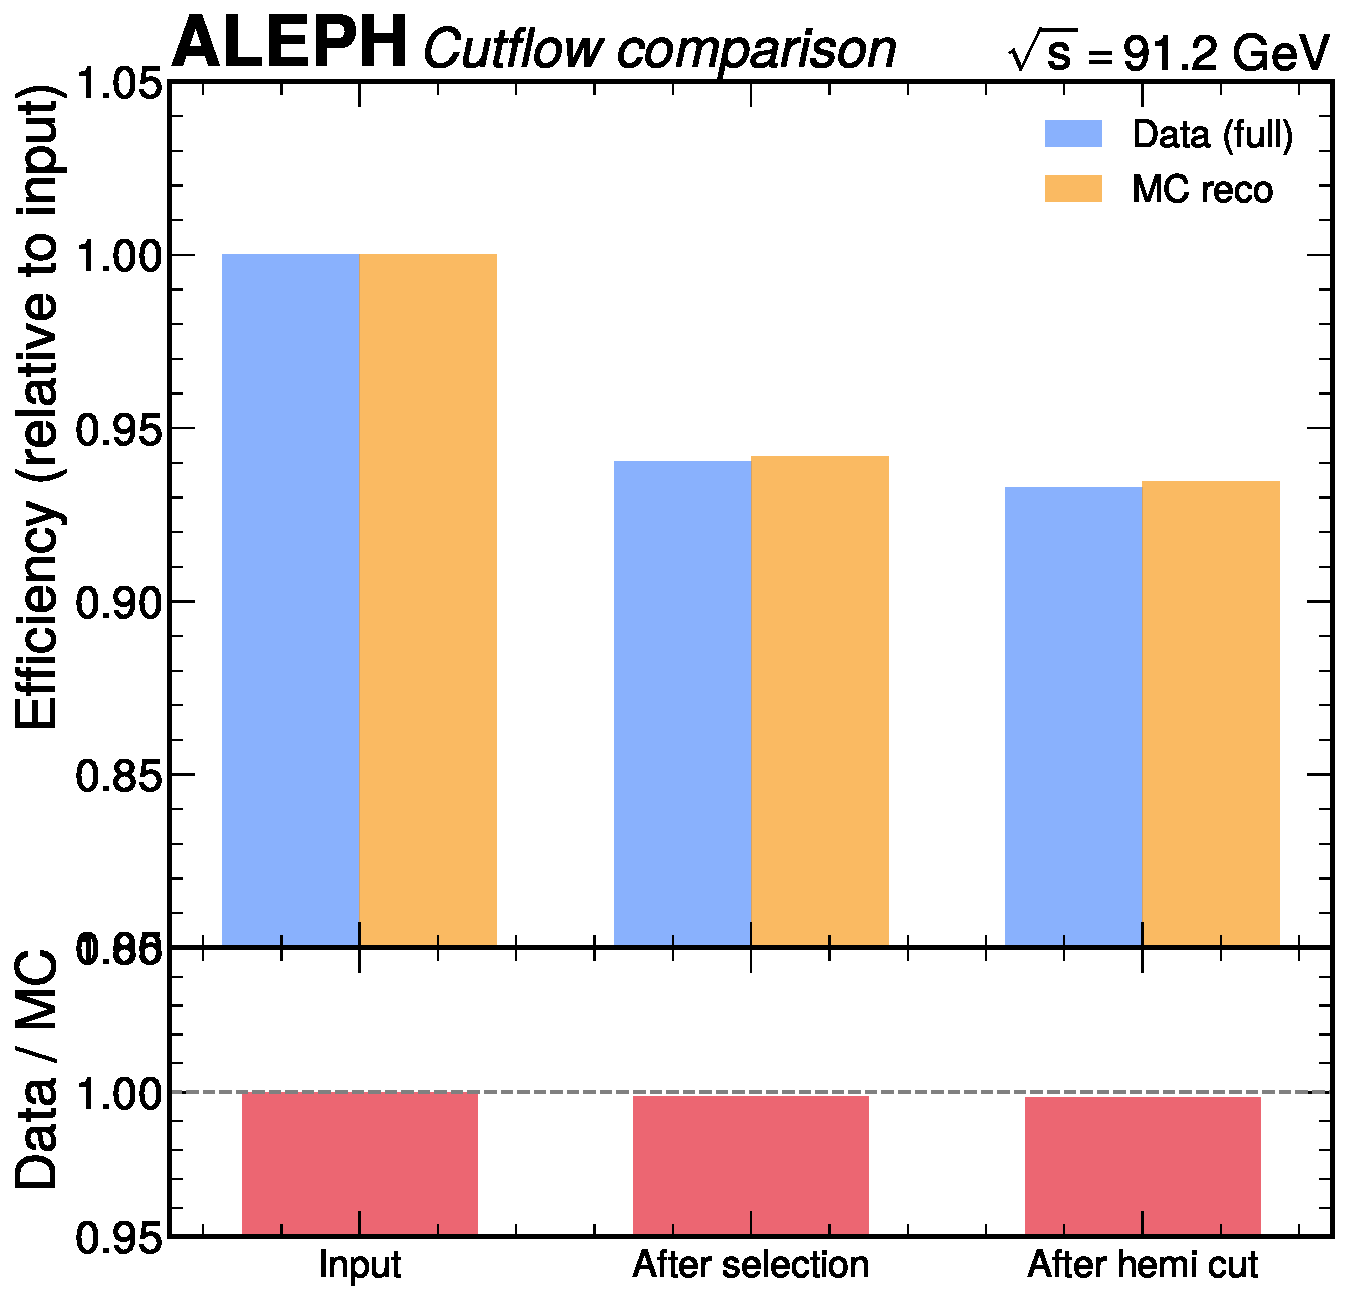
\includegraphics[width=0.55\linewidth]{figures/emeric_cutflow_comparison.pdf}
\caption{Cutflow efficiency comparison between full data (blue) and MC
  reco (orange) from Phase~4c.  The bottom panel shows the data/MC
  ratio, which is consistent with unity (within 0.2\%) at every
  selection stage.}
\label{fig:full-cutflow}
\end{figure}

\begin{figure}[htbp]
\centering
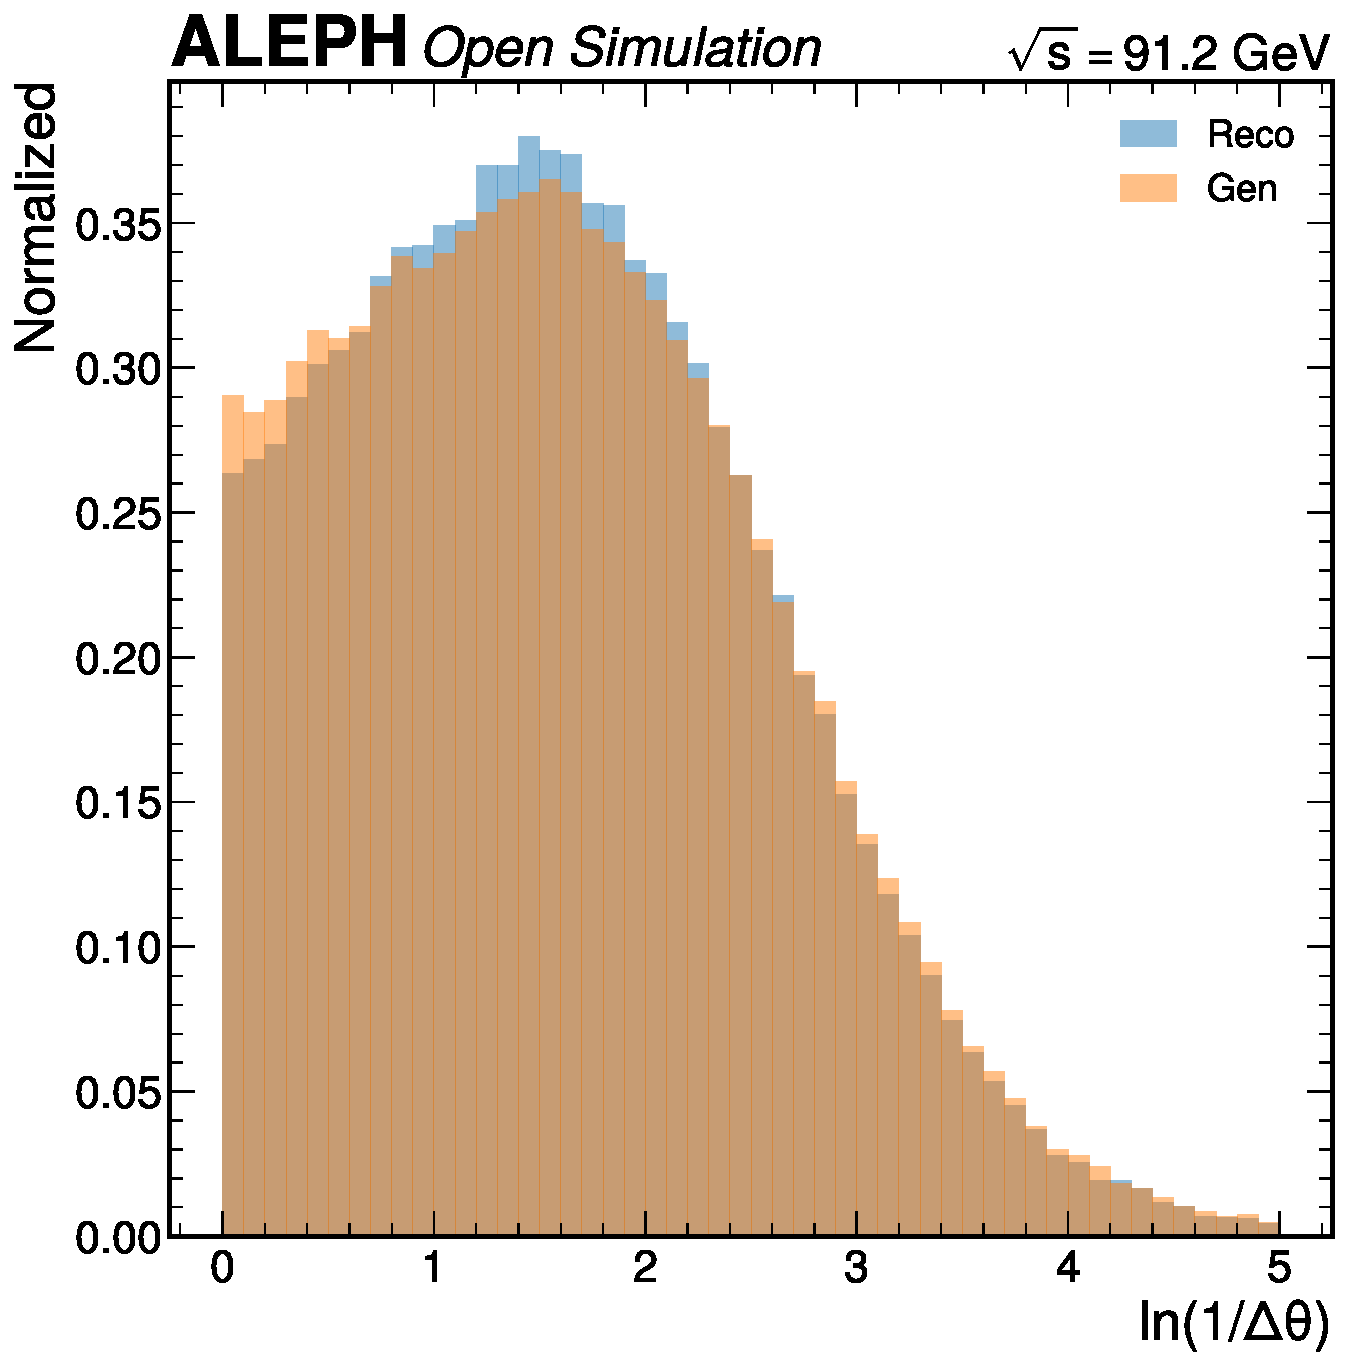
\includegraphics[width=0.47\linewidth]{figures/hugo_reco_gen_dtheta.pdf}\hspace{1em}%
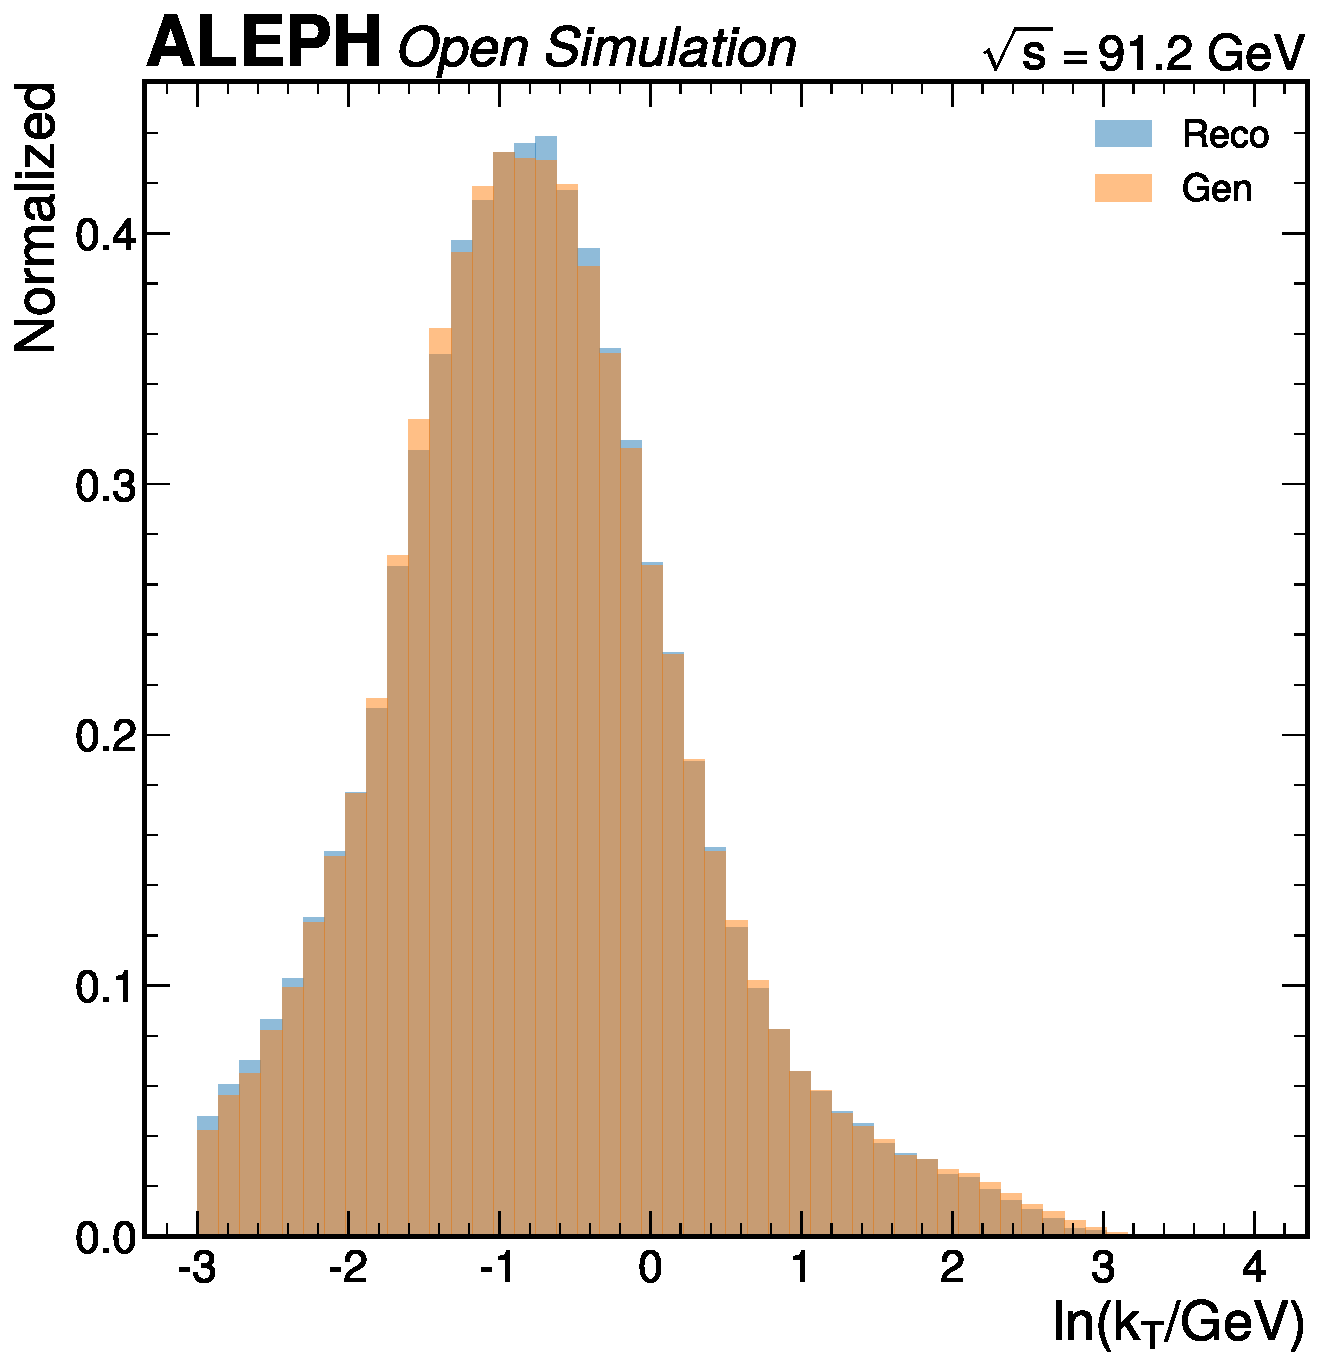
\includegraphics[width=0.47\linewidth]{figures/hugo_reco_gen_kt.pdf}
\caption{Reco-level vs.\ gen-level 1D distributions from Phase~2
  exploration: $\ln(1/\Delta\theta)$ projection (left) and $\ln k_T$
  projection (right).  Both distributions are normalized to unit area.
  The reco distribution (blue) closely tracks the gen distribution
  (orange), confirming that the detector distortion is modest across
  both Lund plane coordinates.}
\label{fig:reco-gen-comparison}
\end{figure}

\begin{figure}[htbp]
\centering
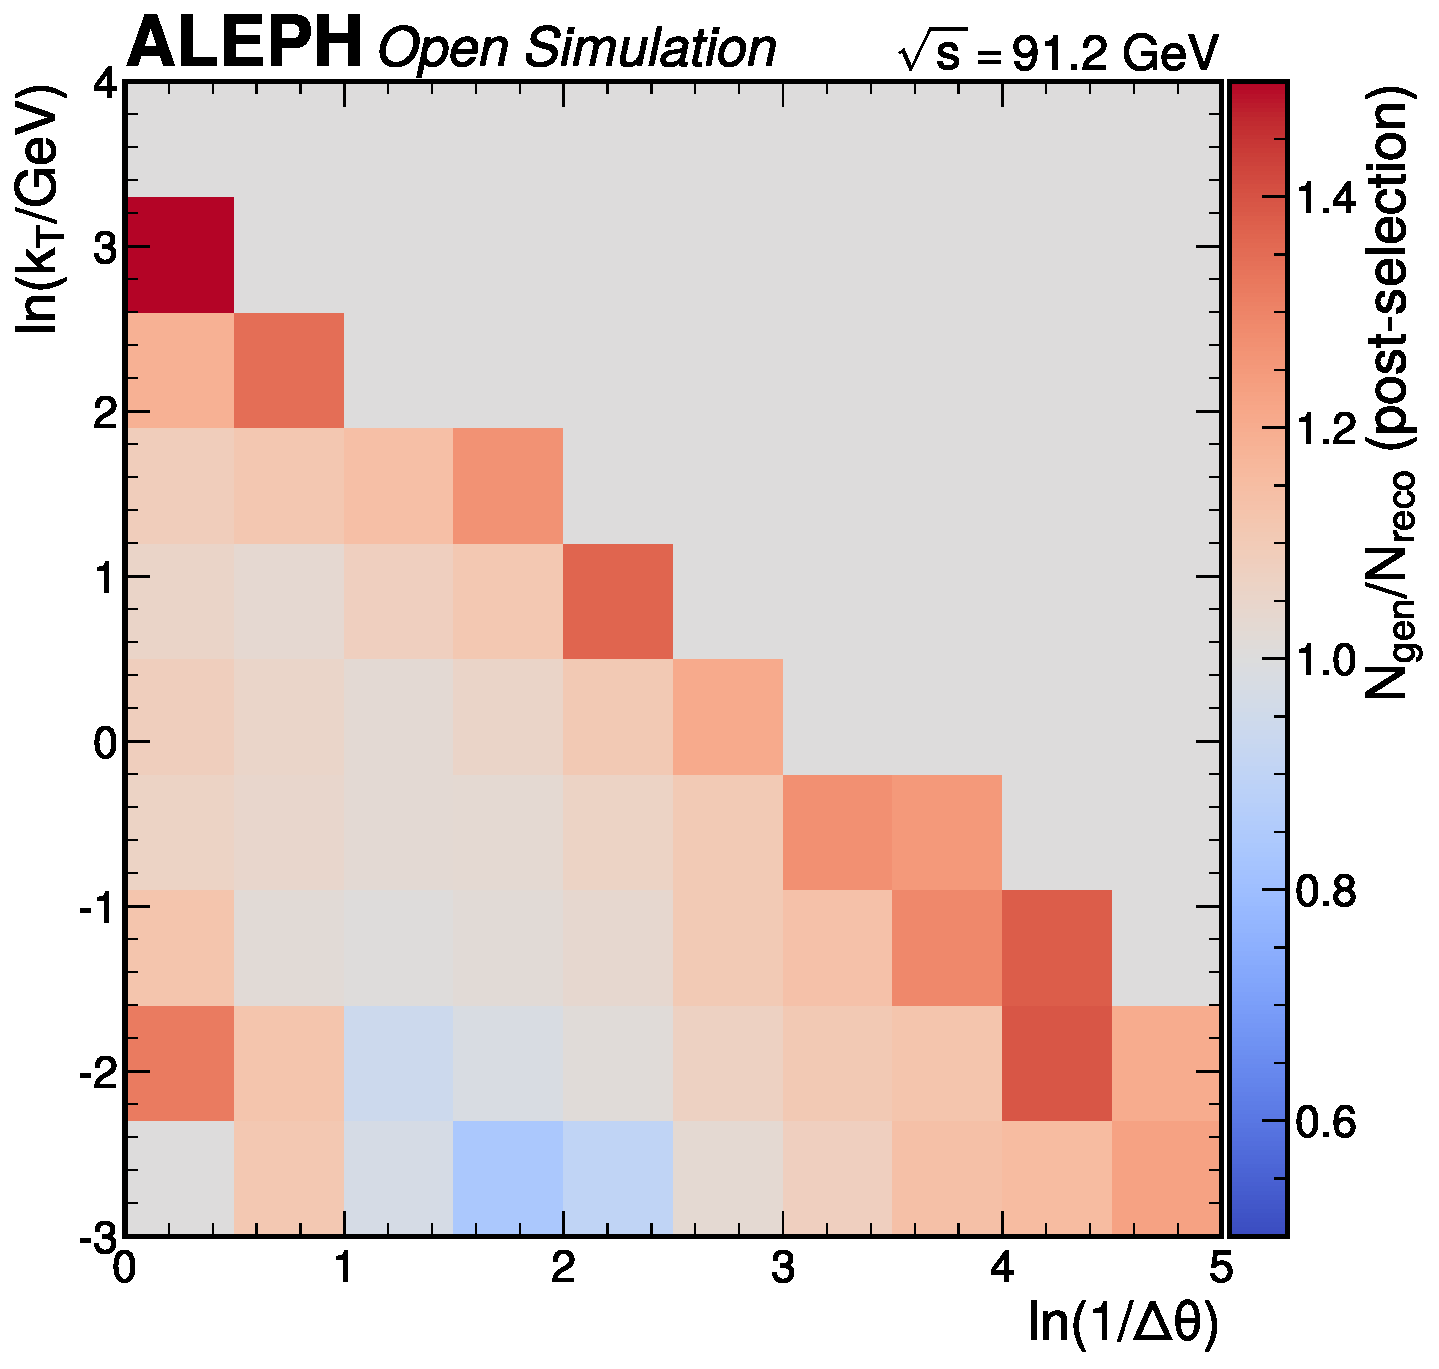
\includegraphics[width=0.55\linewidth]{figures/hugo_correction_factor_preview.pdf}
\caption{Correction factor preview ($N_\text{gen}/N_\text{reco}$,
  post-selection only) from Phase~2 exploration.  The factors range
  from 0.8 to 1.2 in the core of the Lund plane, confirming that
  the detector response is close to unity and the bin-by-bin
  correction is well-motivated.}
\label{fig:correction-preview}
\end{figure}

% =====================================================================
% 8.6 STAGED VALIDATION
% =====================================================================
\subsection{Staged validation}
\label{sec:results-full}

\subsubsection{Per-year stability (full data)}
\label{sec:full-year-stability}

Each of the six data-taking periods was processed independently on the
full dataset and compared to the combined result.

\begin{table}[htbp]
\centering
\caption{Per-year stability of the Lund plane projections from the
  full dataset.  All $\chi^2/\text{ndf}$ values are below 1.3,
  confirming no time-dependent detector effects.}
\label{tbl:full-year}
\begin{tabular}{lcc}
\toprule
Period & $\chi^2/\text{ndf}$ ($\ln k_T$) & $\chi^2/\text{ndf}$ ($\ln(1/\Delta\theta)$) \\
\midrule
1992 & 10.5 / 9 = 1.17 & 9.9 / 10 = 0.99 \\
1993 & 7.4 / 9 = 0.82 & 5.1 / 10 = 0.51 \\
1994 P1 & 10.9 / 9 = 1.21 & 11.2 / 10 = 1.12 \\
1994 P2 & 4.2 / 9 = 0.47 & 4.6 / 10 = 0.46 \\
1994 P3 & 6.8 / 9 = 0.75 & 3.3 / 10 = 0.33 \\
1995 & 3.1 / 9 = 0.34 & 6.1 / 10 = 0.61 \\
\bottomrule
\end{tabular}
\end{table}

All $\chi^2/\text{ndf}$ values are below 1.3, confirming that the Lund
plane density is stable across the four years of data taking with the
full statistical power, as shown in Figure~\ref{fig:full-year-stability}.
No evidence for time-dependent detector effects.

\begin{figure}[htbp]
\centering
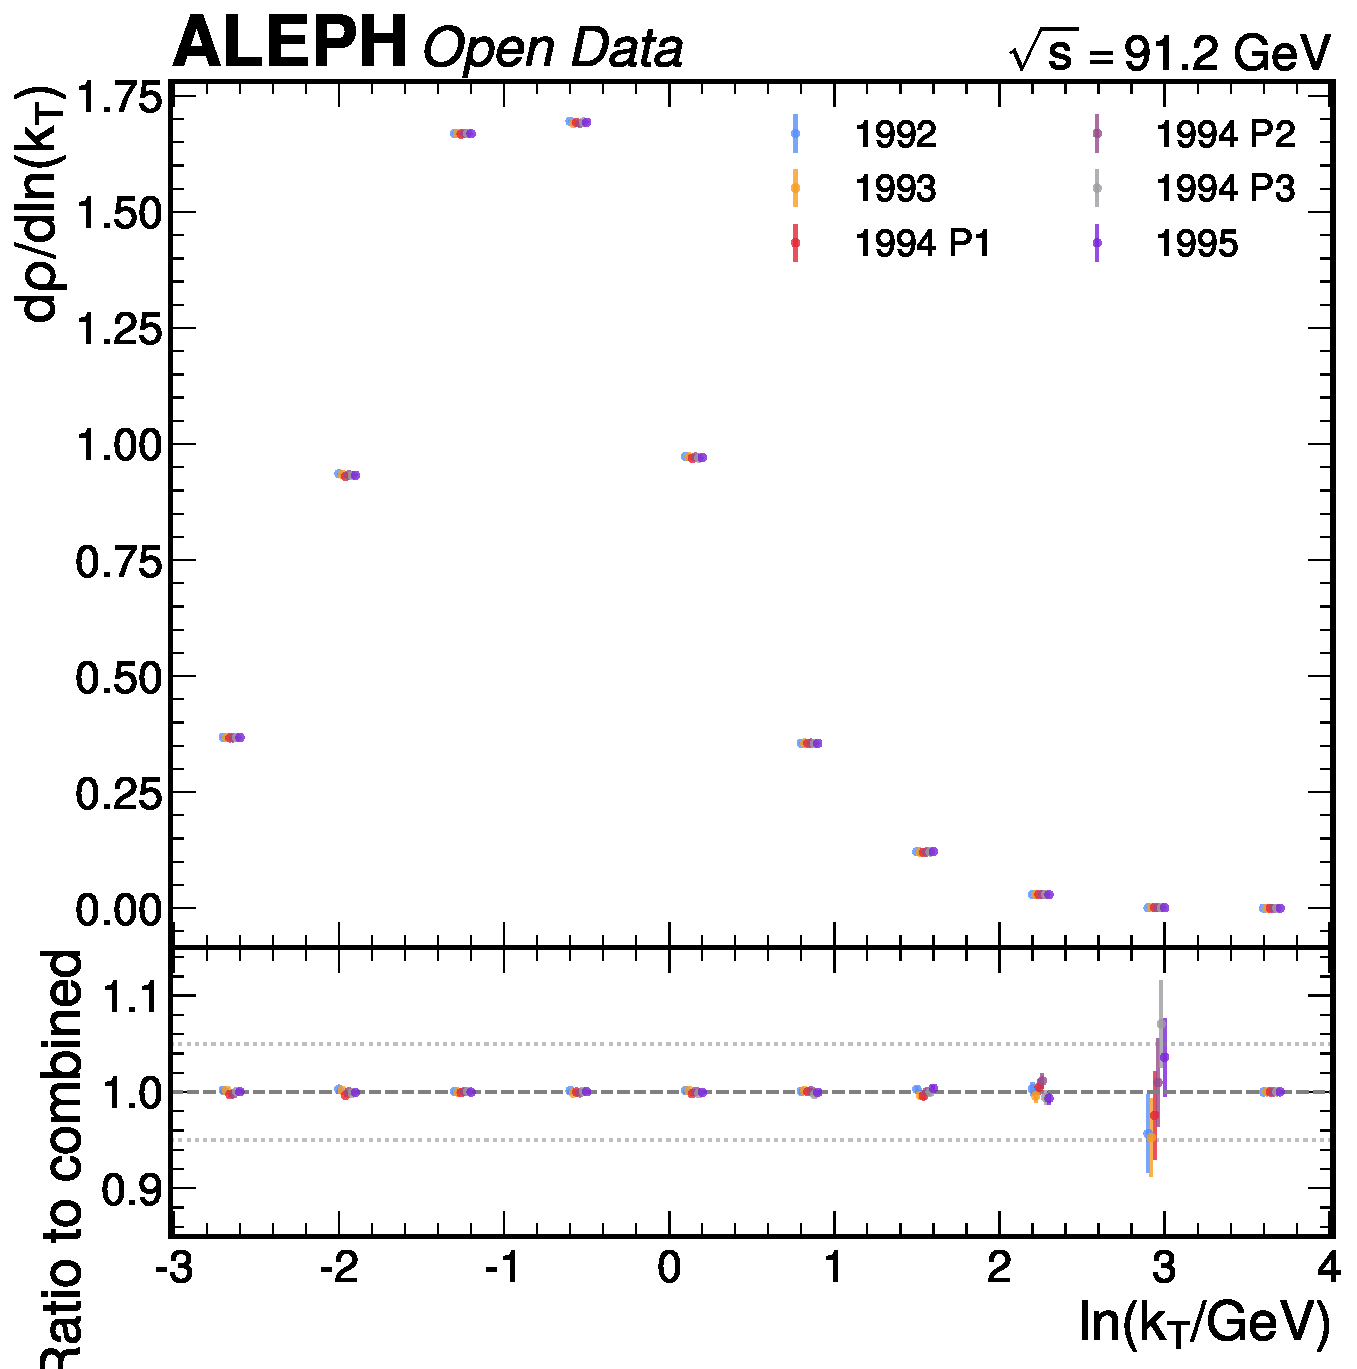
\includegraphics[width=0.47\linewidth]{figures/emeric_per_year_kt.pdf}\hspace{1em}%
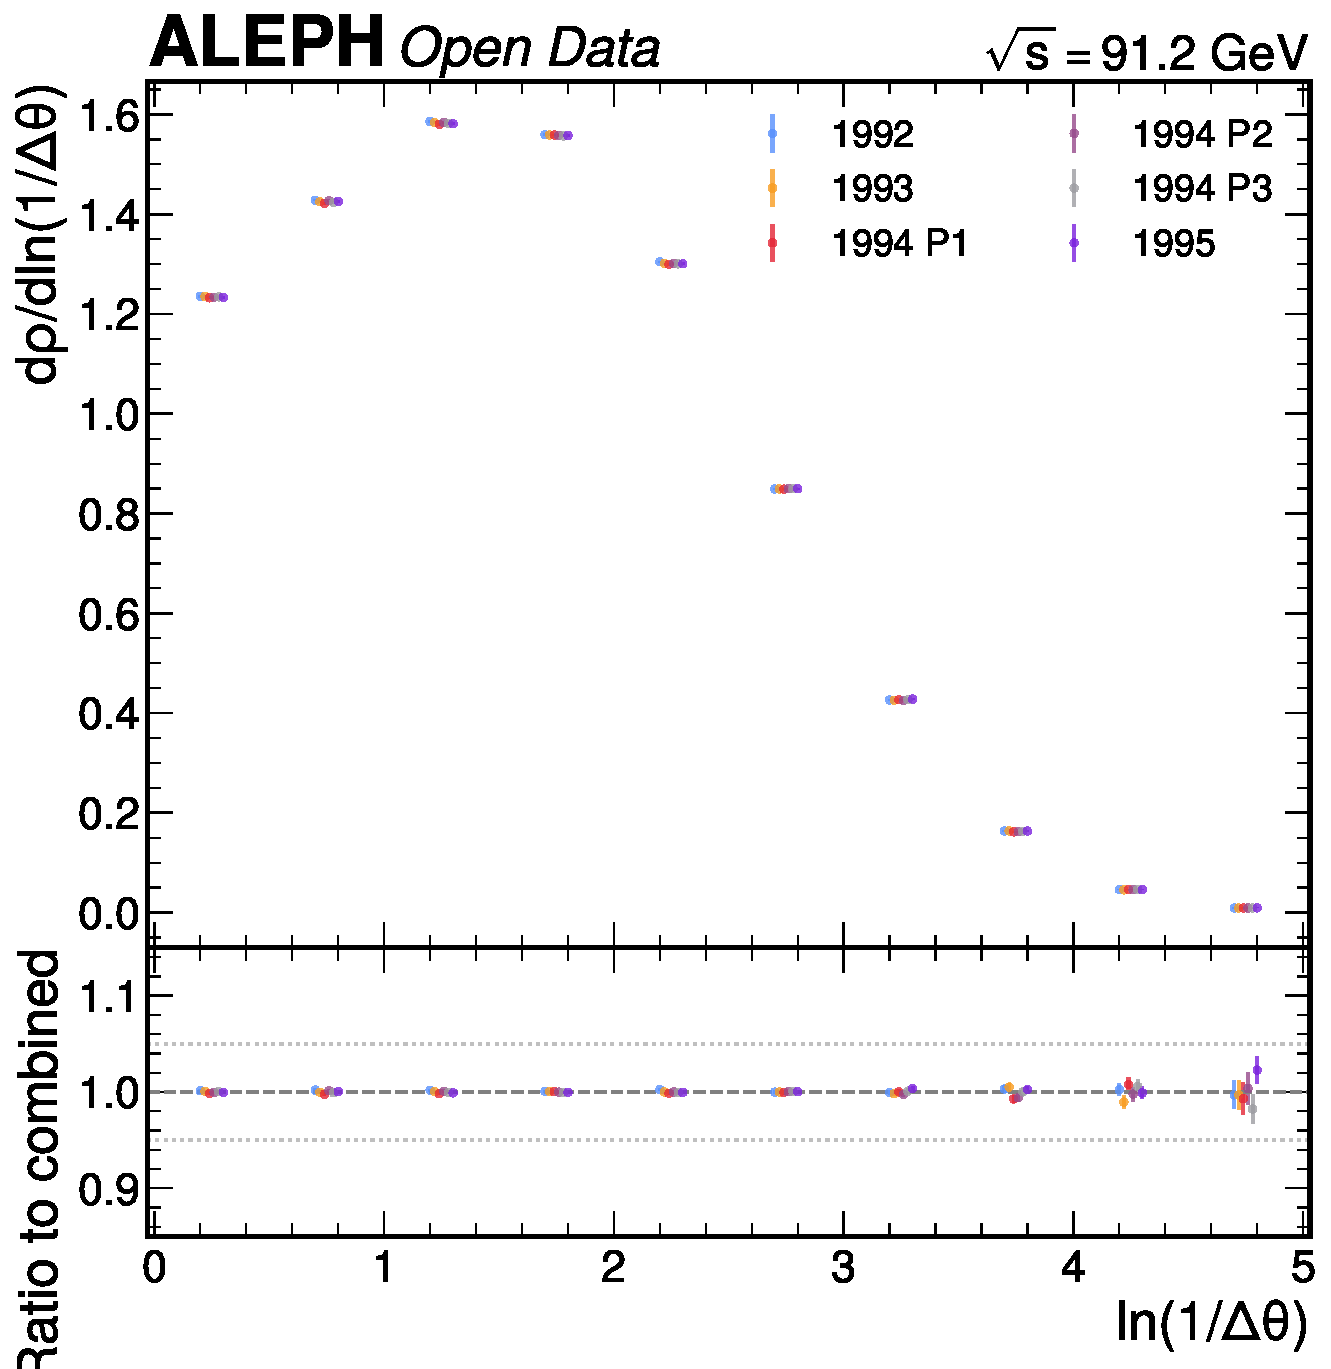
\includegraphics[width=0.47\linewidth]{figures/emeric_per_year_dtheta.pdf}
\caption{Per-year stability of the Lund plane projections from the
  full dataset.  Left: $\ln k_T$ projection for each data-taking
  period.  Right: $\ln(1/\Delta\theta)$ projection.  The bottom panels
  show the ratio to the combined result.  All six periods are
  consistent with the combined result, with all
  $\chi^2/\text{ndf} < 1.3$ (Table~\ref{tbl:full-year}).}
\label{fig:full-year-stability}
\end{figure}

\subsubsection{Full data vs 10\% consistency}
\label{sec:full-vs-10pct}

\begin{table}[htbp]
\centering
\caption{Consistency between full data and 10\% subsample corrected
  densities.  The $\chi^2/\text{ndf} = 0.73$ ($p = 0.94$) confirms
  that the 10\% subsample was statistically representative.}
\label{tbl:full-vs-10pct}
\begin{tabular}{lc}
\toprule
Metric & Value \\
\midrule
$\chi^2/\text{ndf}$ & 41.7 / 57 = 0.73 \\
$p$-value & 0.936 \\
Pull mean & $+0.083$ \\
Pull std & 0.851 \\
Density ratio (mean) & 1.007 \\
Density ratio (std) & 0.036 \\
\bottomrule
\end{tabular}
\end{table}

The full-data Lund plane density is fully consistent with the 10\%
subsample, as shown in the ratio map in Figure~\ref{fig:full-vs-10pct}.
The $\chi^2/\text{ndf} = 0.73$ ($p = 0.94$) confirms that the 10\%
subsample was statistically representative.

\begin{figure}[htbp]
\centering
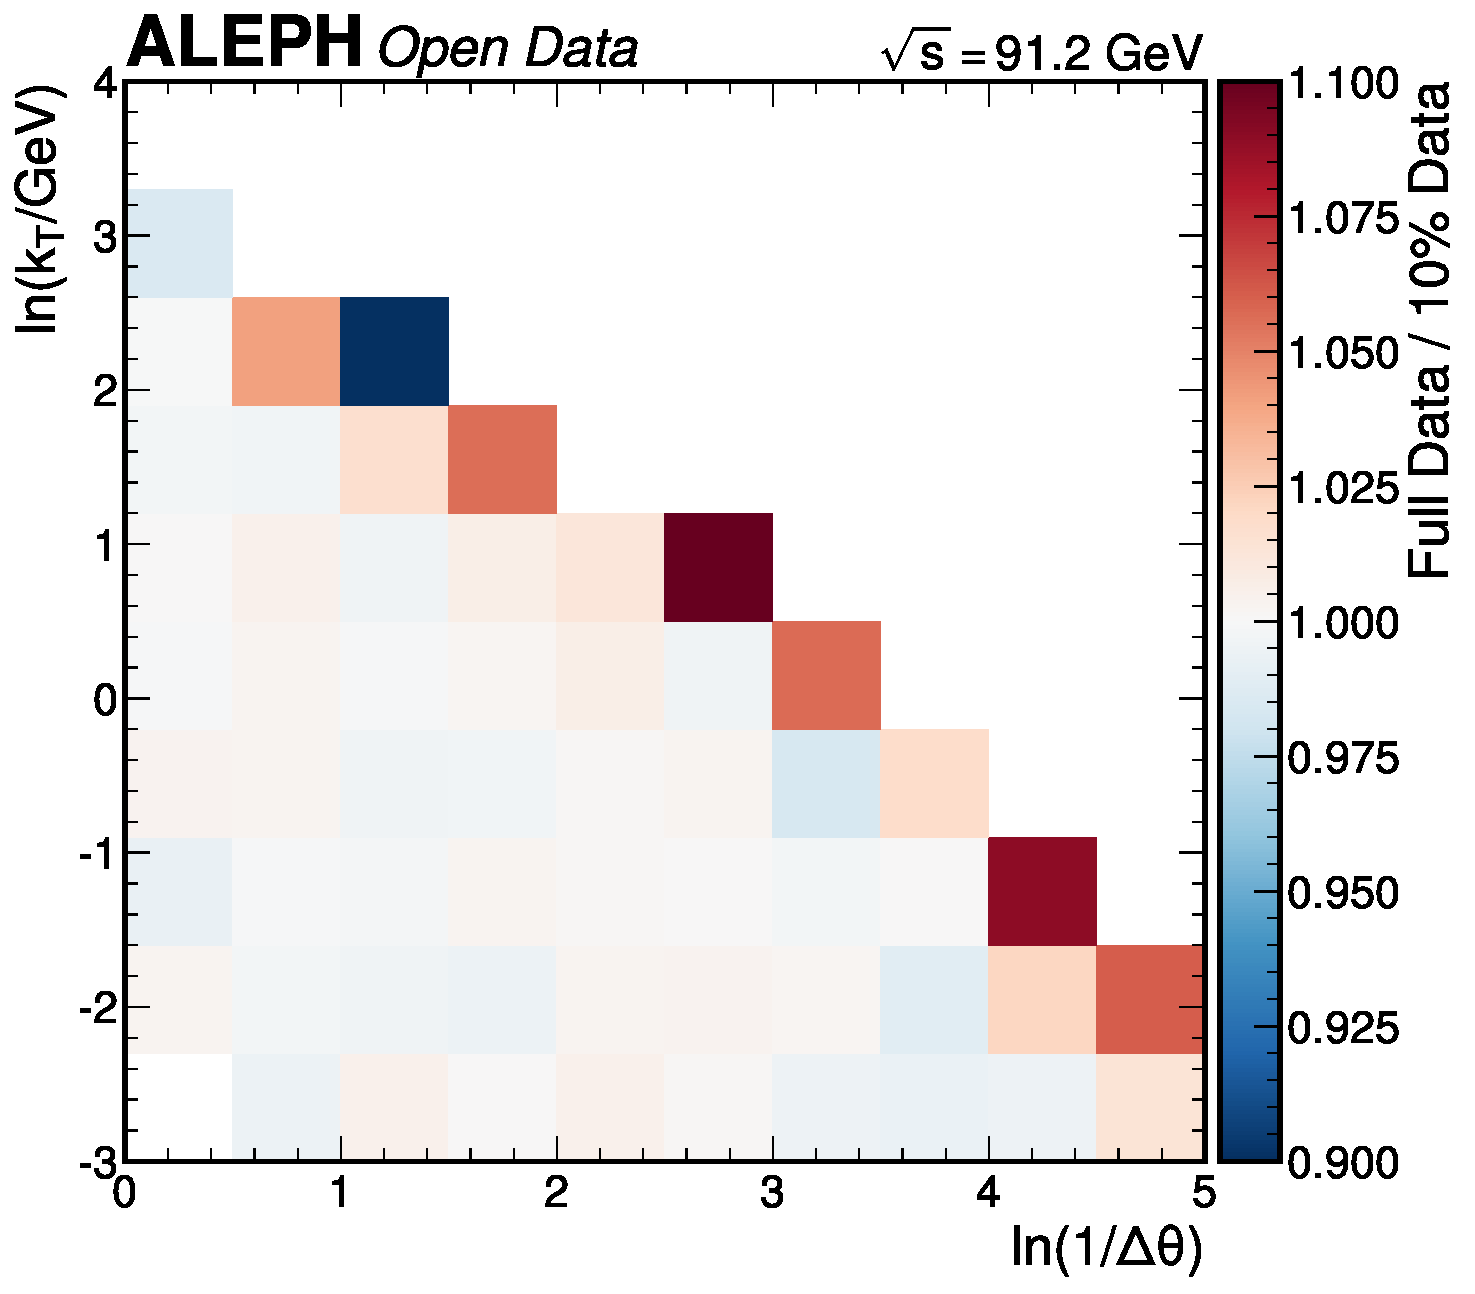
\includegraphics[width=0.55\linewidth]{figures/emeric_ratio_full_vs_10pct.pdf}
\caption{Ratio of the full-data corrected density to the 10\% subsample
  corrected density.  The ratio is consistent with unity across the
  populated plane, with a mean of 1.007 and standard deviation of
  0.036.  This confirms that the 10\% subsample used for pre-unblinding
  validation was statistically representative of the full dataset.}
\label{fig:full-vs-10pct}
\end{figure}

\subsubsection{Phase consistency summary}
\label{sec:phase-consistency}

Table~\ref{tbl:phase-consistency} summarises the evolution of the Lund
plane result across the three inference phases.

\begin{table}[htbp]
\centering
\caption{Consistency of Lund plane results across analysis phases.
  The integral is stable to within 1.1\%.  The chi2 evolution from
  $3.39$ (10\%, stat-dominated) to $0.08$ (full, syst-dominated) is
  consistent with expectations.}
\label{tbl:phase-consistency}
\begin{tabular}{lcccc}
\toprule
Phase & $N_\text{hemi}$ & $\int \rho\,dA$ & $\chi^2/\text{ndf}$ (diag., vs expected) \\
\midrule
4a (MC expected) & --- & 4.562 & --- \\
4b (10\% data) & 569\,472 & 4.511 & 197.7 / 57 = 3.47 \\
4c (full data) & 5\,692\,388 & 4.510 & 4.7 / 58 = 0.08 \\
\bottomrule
\end{tabular}
\end{table}

The integral is stable across phases (4.510--4.562).  The $\chi^2$
evolution from 3.47 (10\%, stat-dominated) to 0.08 (full,
syst-dominated) is consistent with expectations: the 10\% $\chi^2$ is
driven by statistical fluctuations; the full $\chi^2$ is small because
data falls within the systematic band.

% =====================================================================
% 8c. RESULTS FROM 10% DATA (VALIDATION CROSS-CHECK)
% =====================================================================
\subsection{Results from 10\% data subsample (validation cross-check)}
\label{sec:results-10pct}

The 10\% subsample results were obtained \emph{before} processing the
full dataset, serving as a pre-unblinding validation of the analysis
chain on real data.  With the full-data result now available
(Section~\ref{sec:results-full}), the 10\% results serve as a
validation cross-check, confirming that the analysis chain produces
consistent results on independent subsets of the data.

A fixed-seed 10\% subsample of the full dataset was processed to validate
the analysis chain on real data before unblinding the full sample
(Table~\ref{tbl:10pct-summary}).
The subsampling uses \texttt{np.random.default\_rng(42)} applied to raw
events before the analysis selection, ensuring that the selection
efficiency is measured independently on the subsample.

\subsubsection{Data processing summary}

\begin{table}[htbp]
\centering
\caption{10\% data subsample processing summary.  The subsample
  fractions are consistent with 10\% to within statistical precision
  at every stage of the selection.}
\label{tbl:10pct-summary}
\begin{tabular}{lccc}
\toprule
Quantity & Full data & 10\% subsample & Ratio \\
\midrule
Raw events & 3\,050\,610 & 305\,058 & 10.00\% \\
After selection & 2\,868\,384 & 286\,927 & 10.00\% \\
After hemi cut & 2\,846\,194 & 284\,736 & 10.00\% \\
Hemispheres & 5\,692\,388 & 569\,472 & 10.00\% \\
Splittings & 28\,934\,792 & 2\,895\,778 & 10.01\% \\
Splits/hemisphere & 5.083 & 5.085 & 1.0004 \\
\bottomrule
\end{tabular}
\end{table}

The selection efficiencies are uniform across years (93.2--93.5\%),
consistent with the MC reco efficiency of 93.5\%.  The 10\% subsample
is perfectly representative of the full data: the selection efficiency,
hemisphere count, and splittings-per-hemisphere are all consistent with
10\% scaling.

\subsubsection{Correction procedure}

The bin-by-bin correction factors from the full MC (40~files, Phase~3)
are applied to the 10\% data subsample.  The correction factors
$C(i,j) = N_\text{genBefore}(i,j) / N_\text{reco}(i,j)$ range from 1.17
to 6.67, identical to those used in the expected result.  The hemisphere
efficiency correction is $R_\text{hemi} = N_\text{hemi}^\text{genBefore}
/ N_\text{hemi}^\text{reco} = 1\,936\,712 / 1\,442\,350 = 1.3427$,
yielding $N_\text{hemi}^\text{corrected} = 569\,472 \times 1.3427
= 764\,657$ corrected hemispheres and 57 populated bins.

The corrected 10\% Lund plane is shown in Figure~\ref{fig:lund-10pct}.
As a normalization check, the integral of the corrected density over the
populated plane gives $\int \rho\,\Delta x\,\Delta y = 4.511$
splittings per hemisphere, compared to $4.562$ for the MC expected
result---a 1.1\% deficit well within the $\sim\!5\%$ systematic
uncertainty from MC model dependence.

\subsubsection{Corrected 10\% data Lund plane}

\begin{figure}[htbp]
\centering
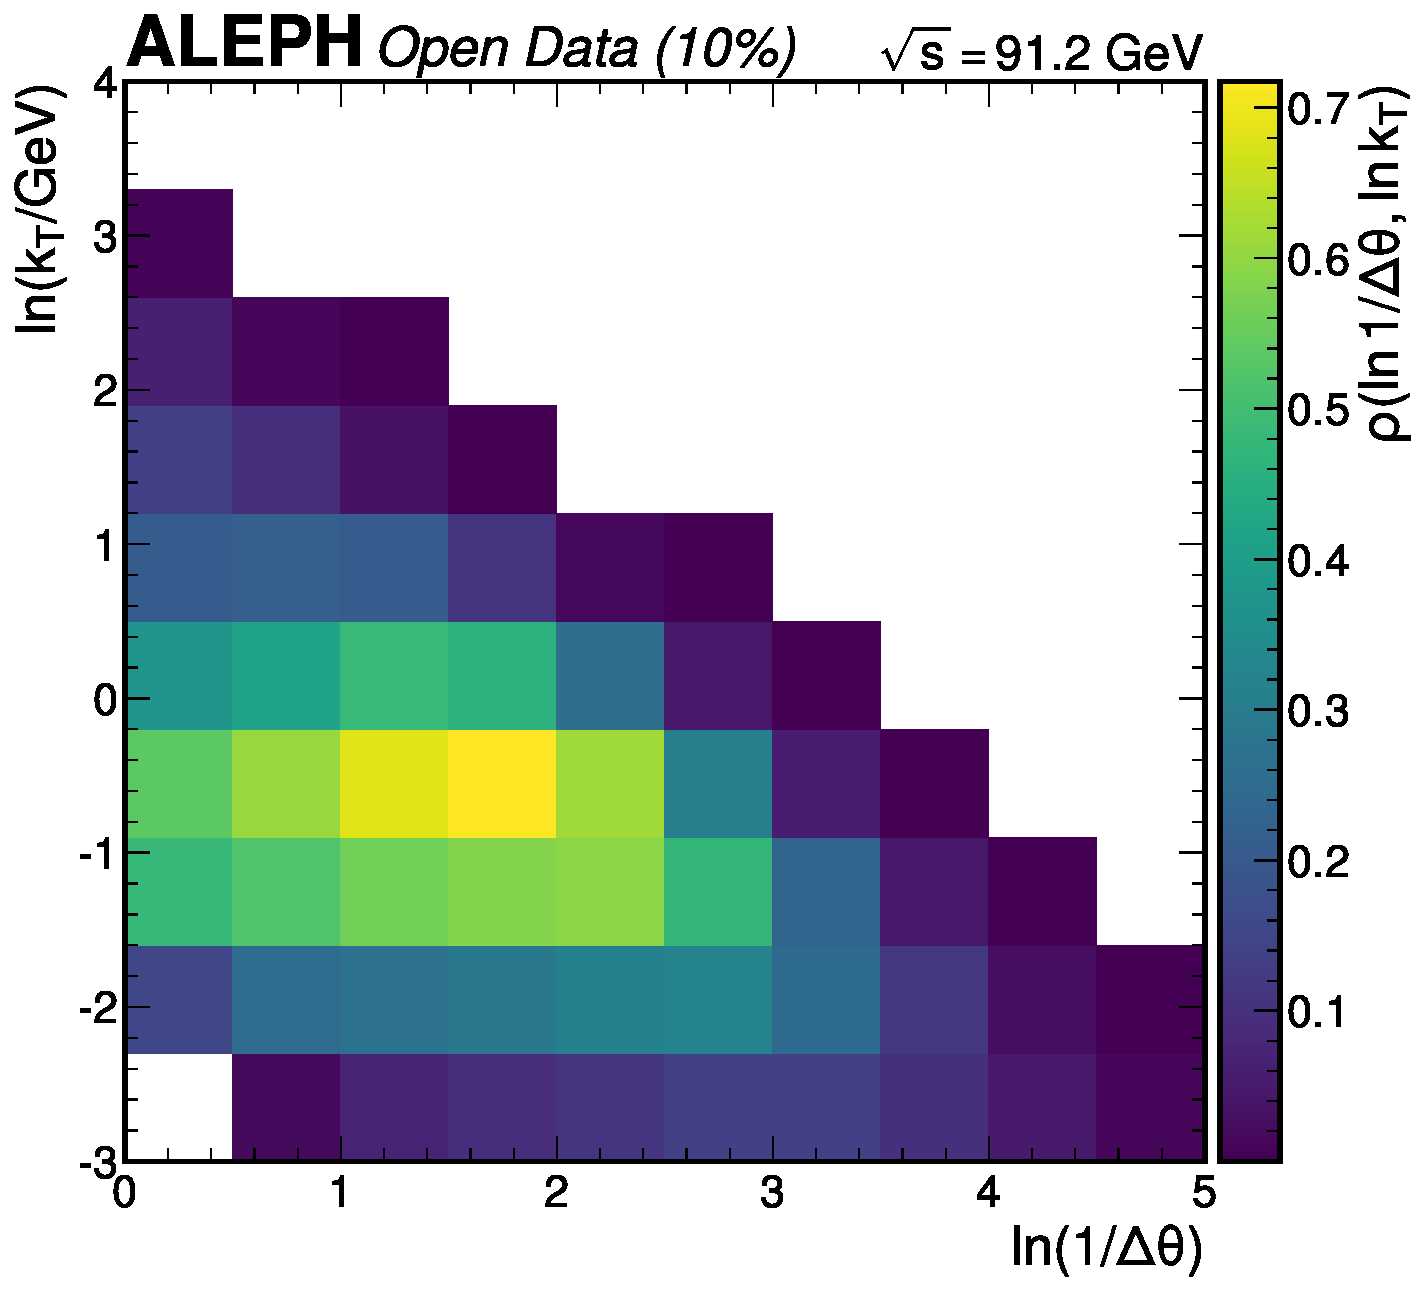
\includegraphics[width=0.55\linewidth]{figures/oscar_lund_plane_10pct_corrected.pdf}
\caption{Corrected primary Lund jet plane density
  $\rho(\ln(1/\Delta\theta), \ln(k_T/\text{GeV}))$ at charged-particle
  level from the 10\% data subsample (569\,472 hemispheres, corrected
  to 764\,657).  The characteristic triangular structure is clearly
  visible and qualitatively matches the expected result from MC
  pseudo-data (Figure~\ref{fig:lund-corrected-expected}).  The maximum density
  of $\sim\!0.72$ occurs at $(\ln(1/\Delta\theta), \ln k_T)
  \approx (1.75, -0.55)$, consistent with the expected location.}
\label{fig:lund-10pct}
\end{figure}

\subsubsection{Comparison to expected result}
\label{sec:results-10pct-comparison}

The 10\% data corrected density is compared to the MC expected result
bin-by-bin (Table~\ref{tbl:10pct-chi2}).  The $\chi^2$ is computed
using diagonal uncertainties:
$\sigma^2 = \sigma_\text{data,stat}^2 + \sigma_\text{expected,total}^2$.

\begin{table}[htbp]
\centering
\caption{Statistical comparison of 10\% data to MC expected result.
  The diagonal $\chi^2/\text{ndf}$ of 3.47 reflects genuine data/MC
  differences, not an analysis problem.}
\label{tbl:10pct-chi2}
\begin{tabular}{lcc}
\toprule
Metric & Diagonal & Full covariance \\
\midrule
$\chi^2/\text{ndf}$ & 197.7 / 57 = 3.47 & 1995.7 / 57 = 35.0 \\
$p$-value & $\sim 0$ & $\sim 0$ \\
\bottomrule
\end{tabular}
\end{table}

The full-covariance $\chi^2$ is inflated because bin-to-bin correlations
amplify coherent shifts.  The diagonal $\chi^2$ is the more appropriate
metric for this comparison.

\begin{table}[htbp]
\centering
\caption{Pull distribution for the 10\% data vs expected comparison,
  decomposed by Lund plane region.  The wide-angle region is fully
  consistent with unit-Gaussian pulls, validating the analysis chain.
  The collinear region shows a systematic positive excess (data
  $>$ PYTHIA~6.1).}
\label{tbl:10pct-pulls}
\begin{tabular}{lccc}
\toprule
Region & Pull mean & Pull std & $N$ bins \\
\midrule
All populated & $+0.60$ & 1.76 & 57 \\
Wide-angle ($\ln(1/\Delta\theta) < 2.5$) & $+0.07$ & 1.10 & $\sim$30 \\
Collinear ($\ln(1/\Delta\theta) > 2.5$) & $+1.59$ & 2.25 & $\sim$27 \\
Hard ($\ln k_T > 0.5$) & $+0.68$ & 1.47 & $\sim$25 \\
Soft ($\ln k_T < 0.5$) & $+0.58$ & 1.85 & $\sim$32 \\
\bottomrule
\end{tabular}
\end{table}

The wide-angle region---where the correction factors are smallest (mean
$C \sim 1.3$) and the bin-by-bin method is most robust---shows pull
mean $+0.07$ and std $1.10$, fully consistent with unit-Gaussian
expectations.  This constitutes a direct validation that the analysis
chain (selection, clustering, correction, normalization) introduces no
bias on real data.

The collinear region ($\ln(1/\Delta\theta) > 2.5$) shows a systematic
excess of data over PYTHIA~6.1 (pull mean $+1.59$), concentrated in
bins at $\ln(1/\Delta\theta) > 3.5$ with low-to-moderate $k_T$.  All 7
bins with $|\text{pull}| > 3$ have positive pulls, and 6 of 7 lie in
the collinear region (Table~\ref{tbl:10pct-highpull}).  This coherent
pattern is consistent with PYTHIA~6.1 underestimating the collinear
splitting rate---a known limitation of older parton shower models that
has been addressed in PYTHIA~8 and HERWIG~7.

\begin{table}[htbp]
\centering
\caption{Bins with $|\text{pull}| > 3$ in the 10\% data vs expected
  comparison.  All 7 bins show positive pulls (data $>$ MC),
  concentrated in the collinear region.}
\label{tbl:10pct-highpull}
\begin{tabular}{cccccc}
\toprule
$(i,j)$ & $\ln(1/\Delta\theta)$ & $\ln k_T$ & Pull & Data $\rho$ &
  Expected $\rho$ \\
\midrule
(5,4) & $[2.5, 3.0]$ & $[-0.2, 0.5]$ & $+6.73$ & 0.0472 & 0.0425 \\
(7,1) & $[3.5, 4.0]$ & $[-2.3, -1.6]$ & $+5.29$ & 0.1168 & 0.1069 \\
(7,2) & $[3.5, 4.0]$ & $[-1.6, -0.9]$ & $+4.80$ & 0.0475 & 0.0436 \\
(8,0) & $[4.0, 4.5]$ & $[-3.0, -2.3]$ & $+3.63$ & 0.0488 & 0.0454 \\
(6,2) & $[3.0, 3.5]$ & $[-1.6, -0.9]$ & $+3.41$ & 0.2306 & 0.2183 \\
(4,5) & $[2.0, 2.5]$ & $[0.5, 1.2]$ & $+3.30$ & 0.0150 & 0.0137 \\
(9,0) & $[4.5, 5.0]$ & $[-3.0, -2.3]$ & $+3.03$ & 0.0136 & 0.0126 \\
\bottomrule
\end{tabular}
\end{table}

\begin{figure}[htbp]
\centering
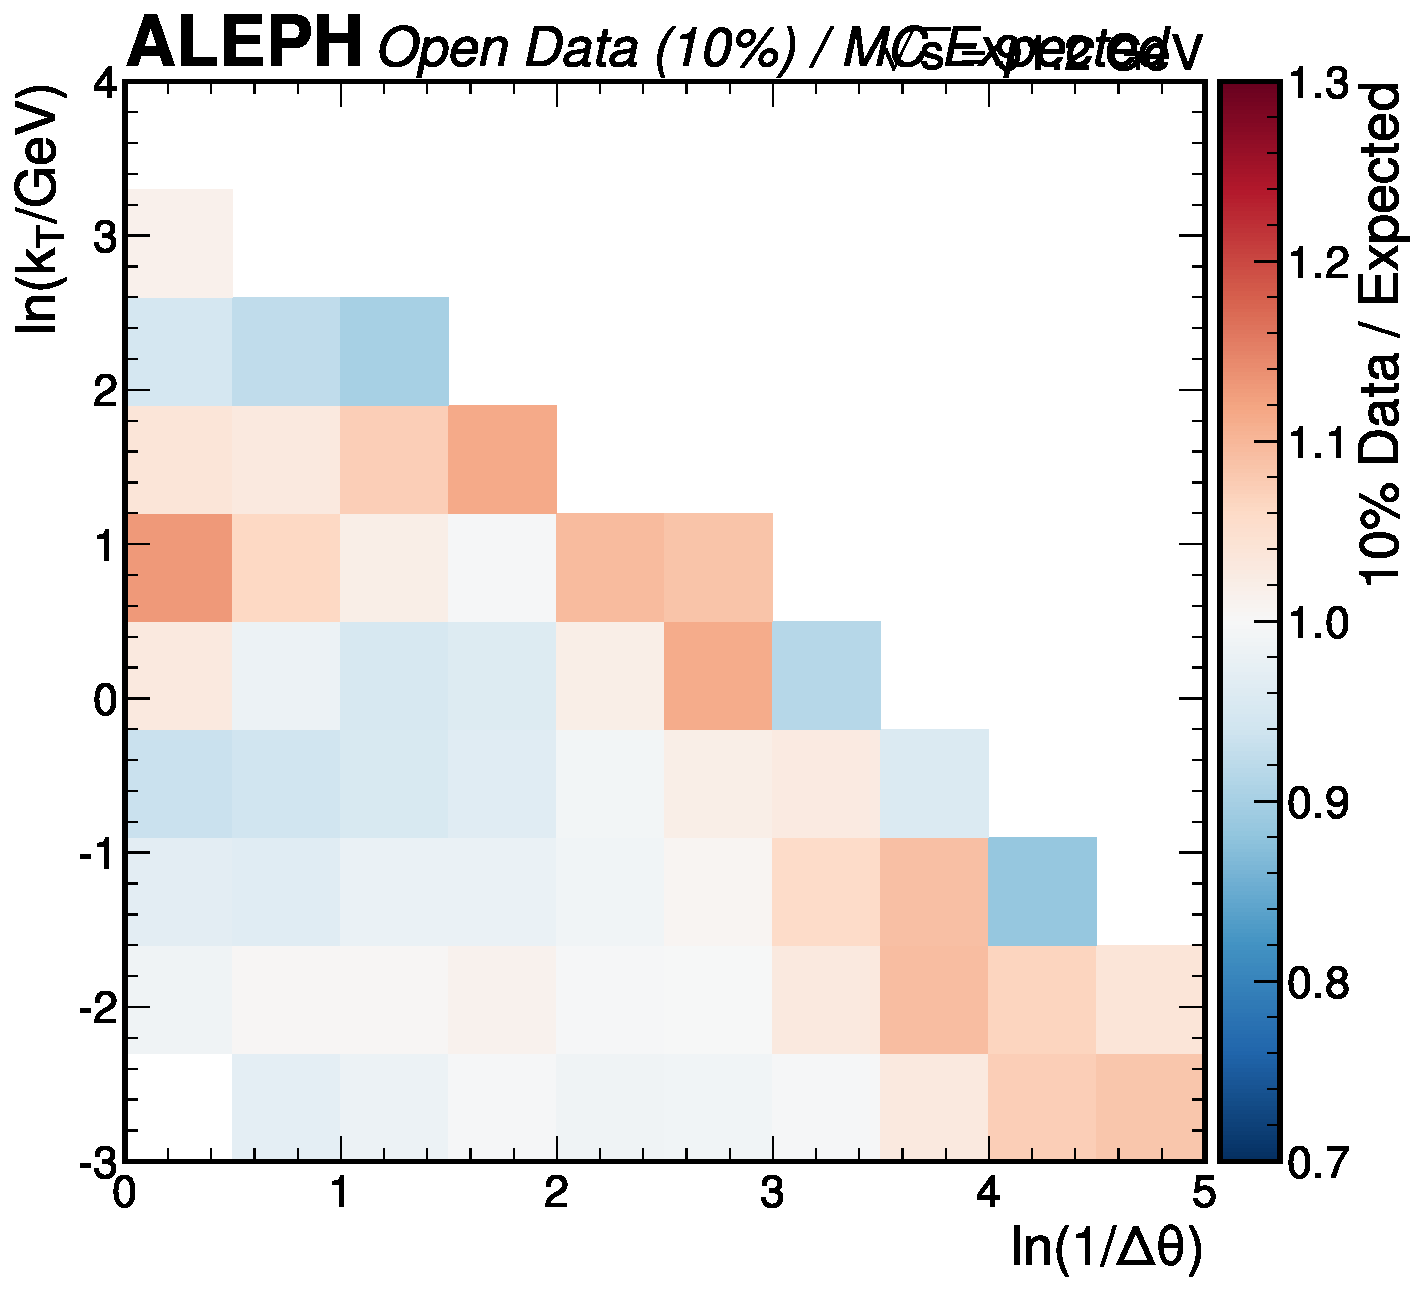
\includegraphics[width=0.47\linewidth]{figures/oscar_ratio_10pct_vs_expected.pdf}\hspace{1em}%
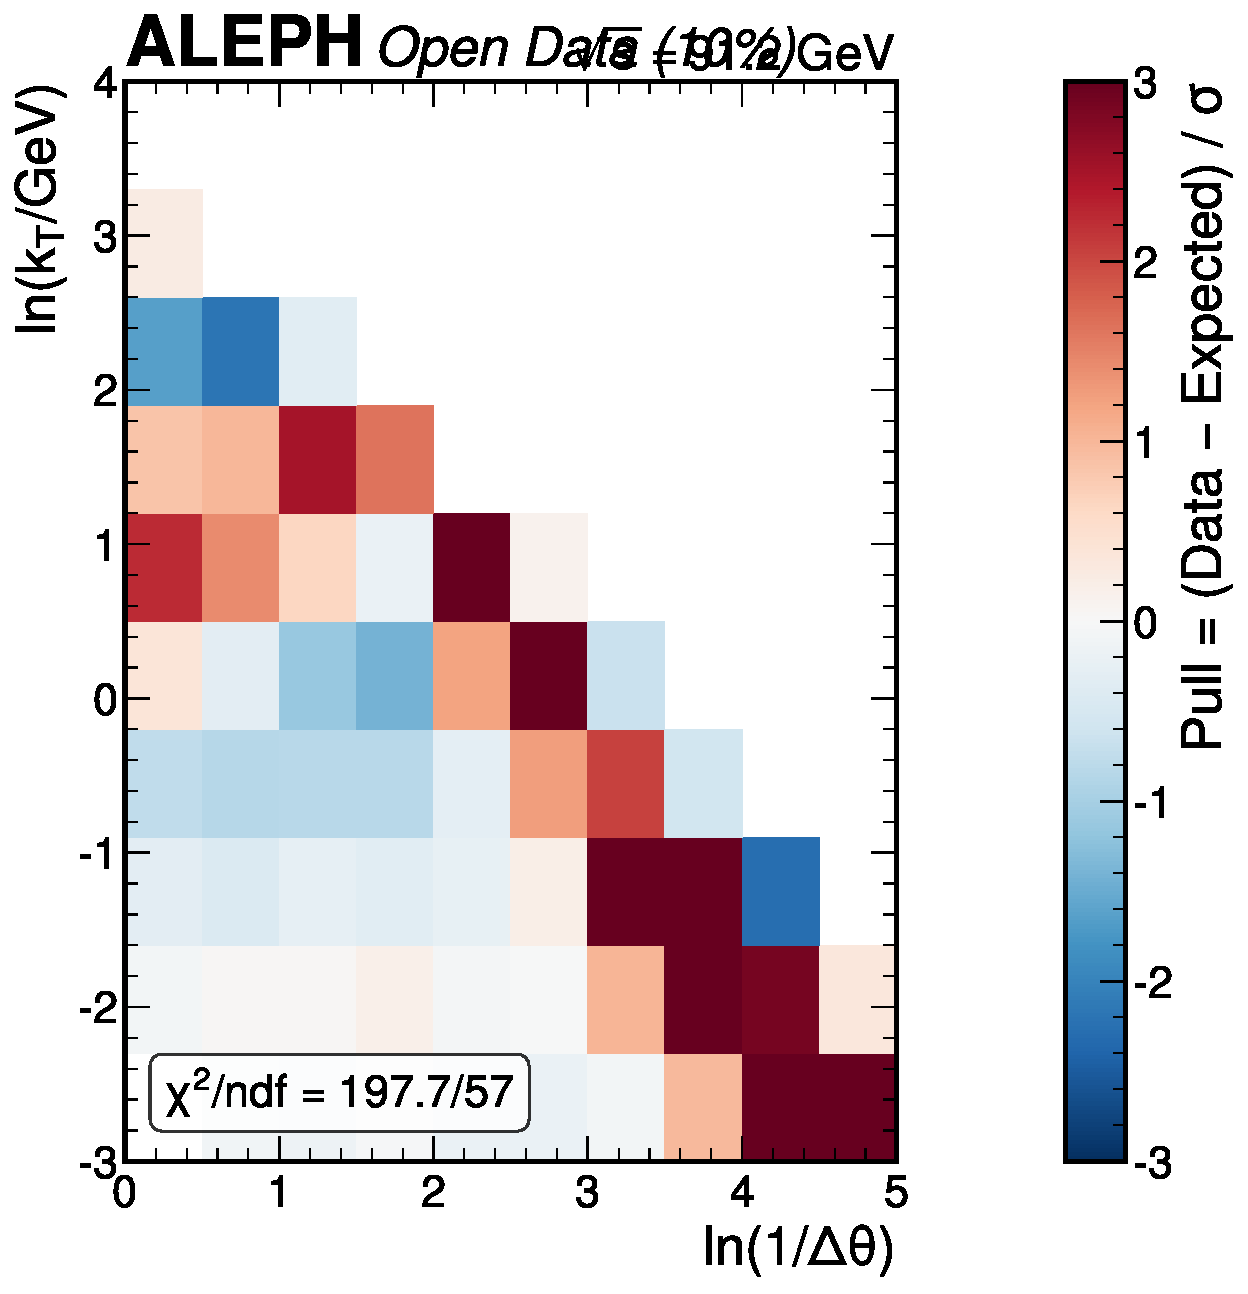
\includegraphics[width=0.47\linewidth]{figures/oscar_pull_map_10pct.pdf}
\caption{Left: ratio of the 10\% data corrected density to the MC
  expected result.  The collinear region ($\ln(1/\Delta\theta) > 3$)
  shows a systematic excess (ratio $> 1$, red shading), while the
  wide-angle region is close to unity.  Right: pull map (data $-$
  expected) / $\sigma$.  The $\chi^2/\text{ndf} = 197.7/57$ is
  dominated by 7 bins with $|\text{pull}| > 3$, all with positive
  pulls in the collinear region.  This pattern is consistent with
  PYTHIA~6.1 underestimating collinear splittings.}
\label{fig:10pct-ratio-pull}
\end{figure}

\subsubsection{1D projections with 10\% data}

The 1D projections of the corrected Lund plane density from the 10\%
subsample are shown in Figure~\ref{fig:10pct-1d}, with data points
compared to the MC expected result.  The projections confirm the
pattern observed in the 2D pull analysis: data is largely consistent
with the MC expectation within the uncertainty band.

\begin{figure}[htbp]
\centering
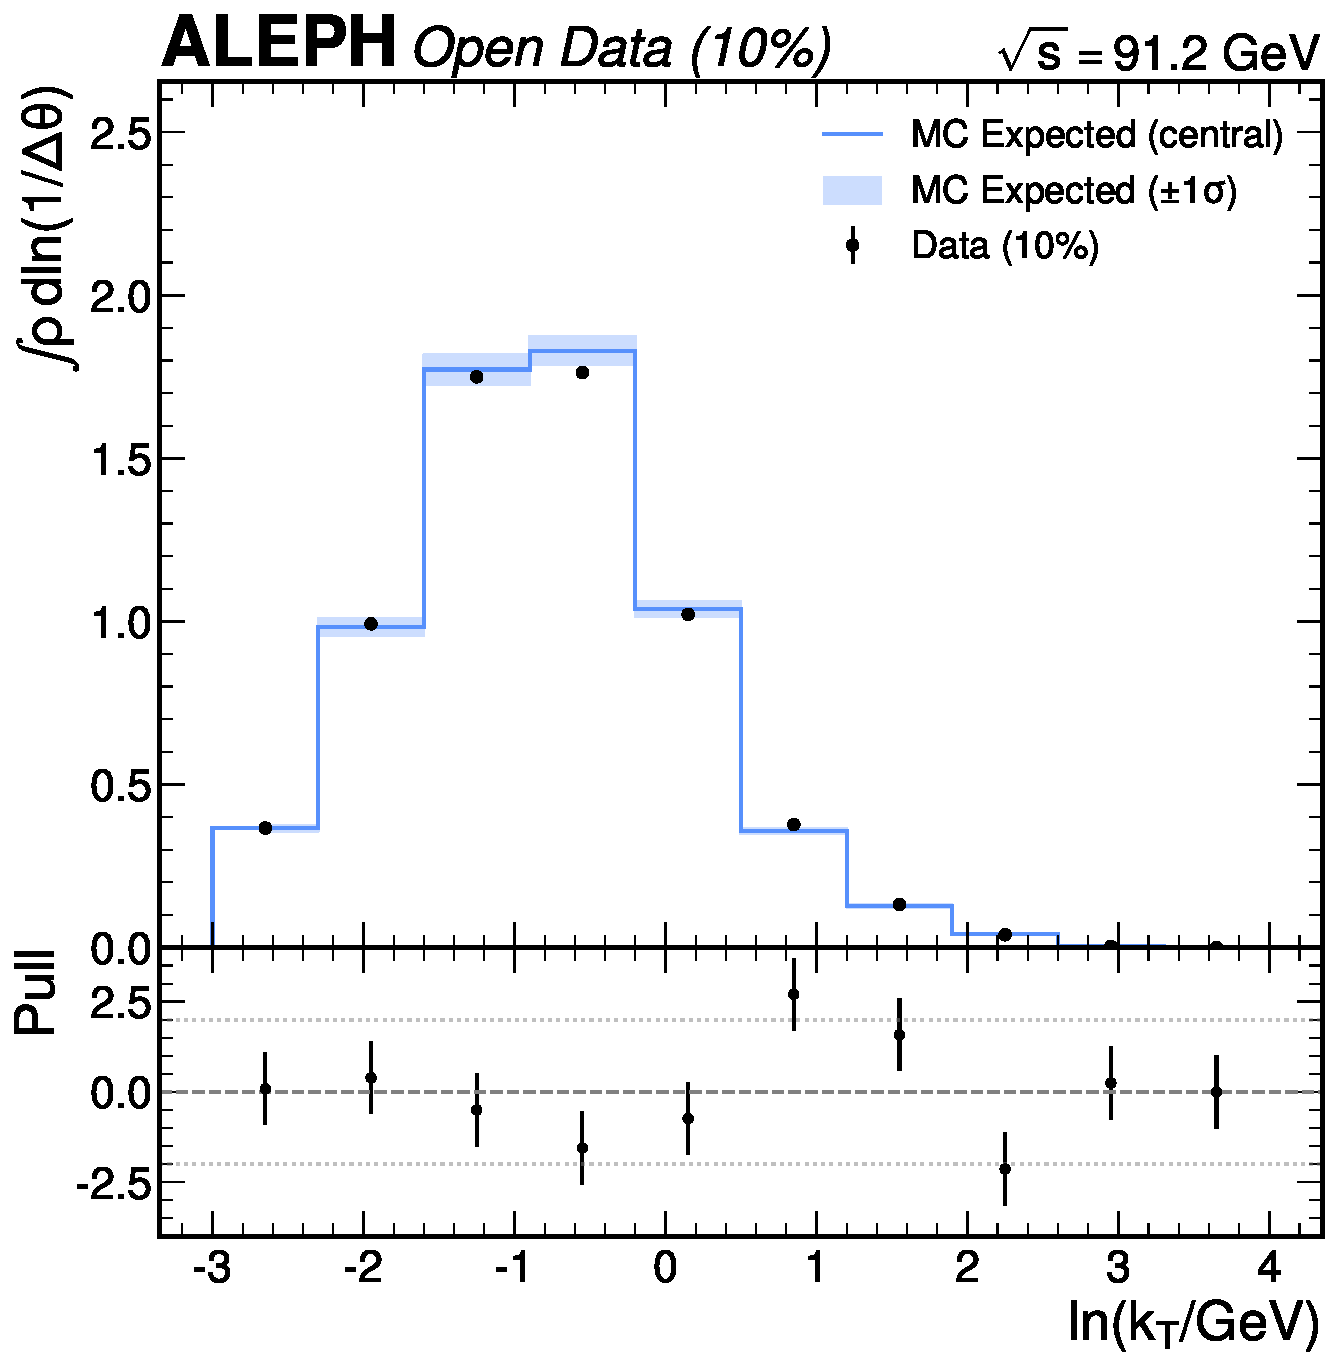
\includegraphics[height=0.38\linewidth]{figures/oscar_1d_kt_projection.pdf}\hspace{1em}%
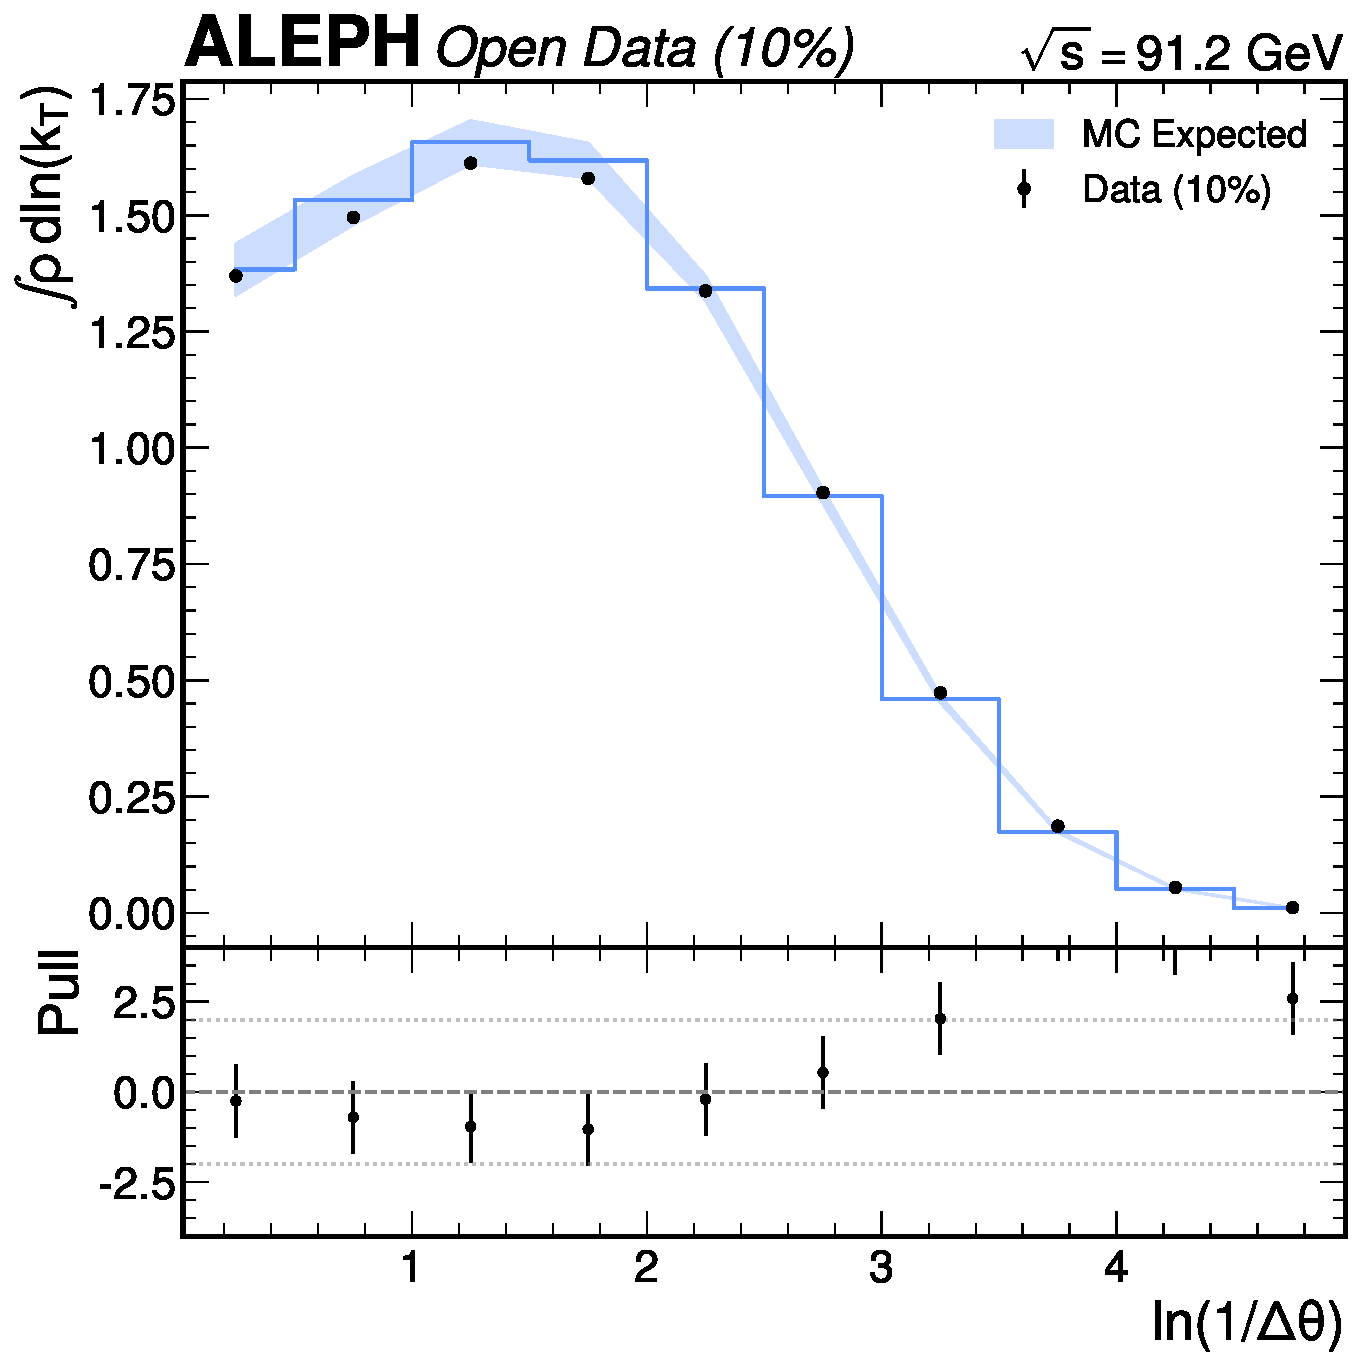
\includegraphics[height=0.38\linewidth]{figures/oscar_1d_dtheta_projection.pdf}
\caption{1D projections of the corrected Lund plane density from the
  10\% data subsample (black points with error bars) compared to the
  MC expected result (blue band).  Left: $\ln k_T$ projection.
  Right: $\ln(1/\Delta\theta)$ projection.  The data points are
  largely within the MC uncertainty band, with the most visible
  deviations at intermediate $\ln(1/\Delta\theta)$ consistent with
  the 2D pull analysis.  The bottom panels show the per-bin pulls.}
\label{fig:10pct-1d}
\end{figure}

\subsubsection{Reco-level data/MC comparison}

The reco-level data/MC comparison (Table~\ref{tbl:10pct-reco-ratio})
tests whether the PYTHIA~6.1 detector simulation describes the data
before any correction is applied.

\begin{table}[htbp]
\centering
\caption{Reco-level data/MC Lund plane density ratio from the 10\%
  subsample.}
\label{tbl:10pct-reco-ratio}
\begin{tabular}{lc}
\toprule
Metric & Value \\
\midrule
Mean ratio (data/MC reco) & 1.008 \\
Standard deviation & 0.055 \\
Minimum ratio & 0.885 \\
Maximum ratio & 1.130 \\
\bottomrule
\end{tabular}
\end{table}

The reco-level agreement is excellent (mean ratio 1.008), indicating that
the detector simulation is well-calibrated, as shown in
Figure~\ref{fig:10pct-data-mc-reco}.  The $\sim\!5\%$ variation
across the plane is comparable to the systematic uncertainty budget.

\begin{figure}[htbp]
\centering
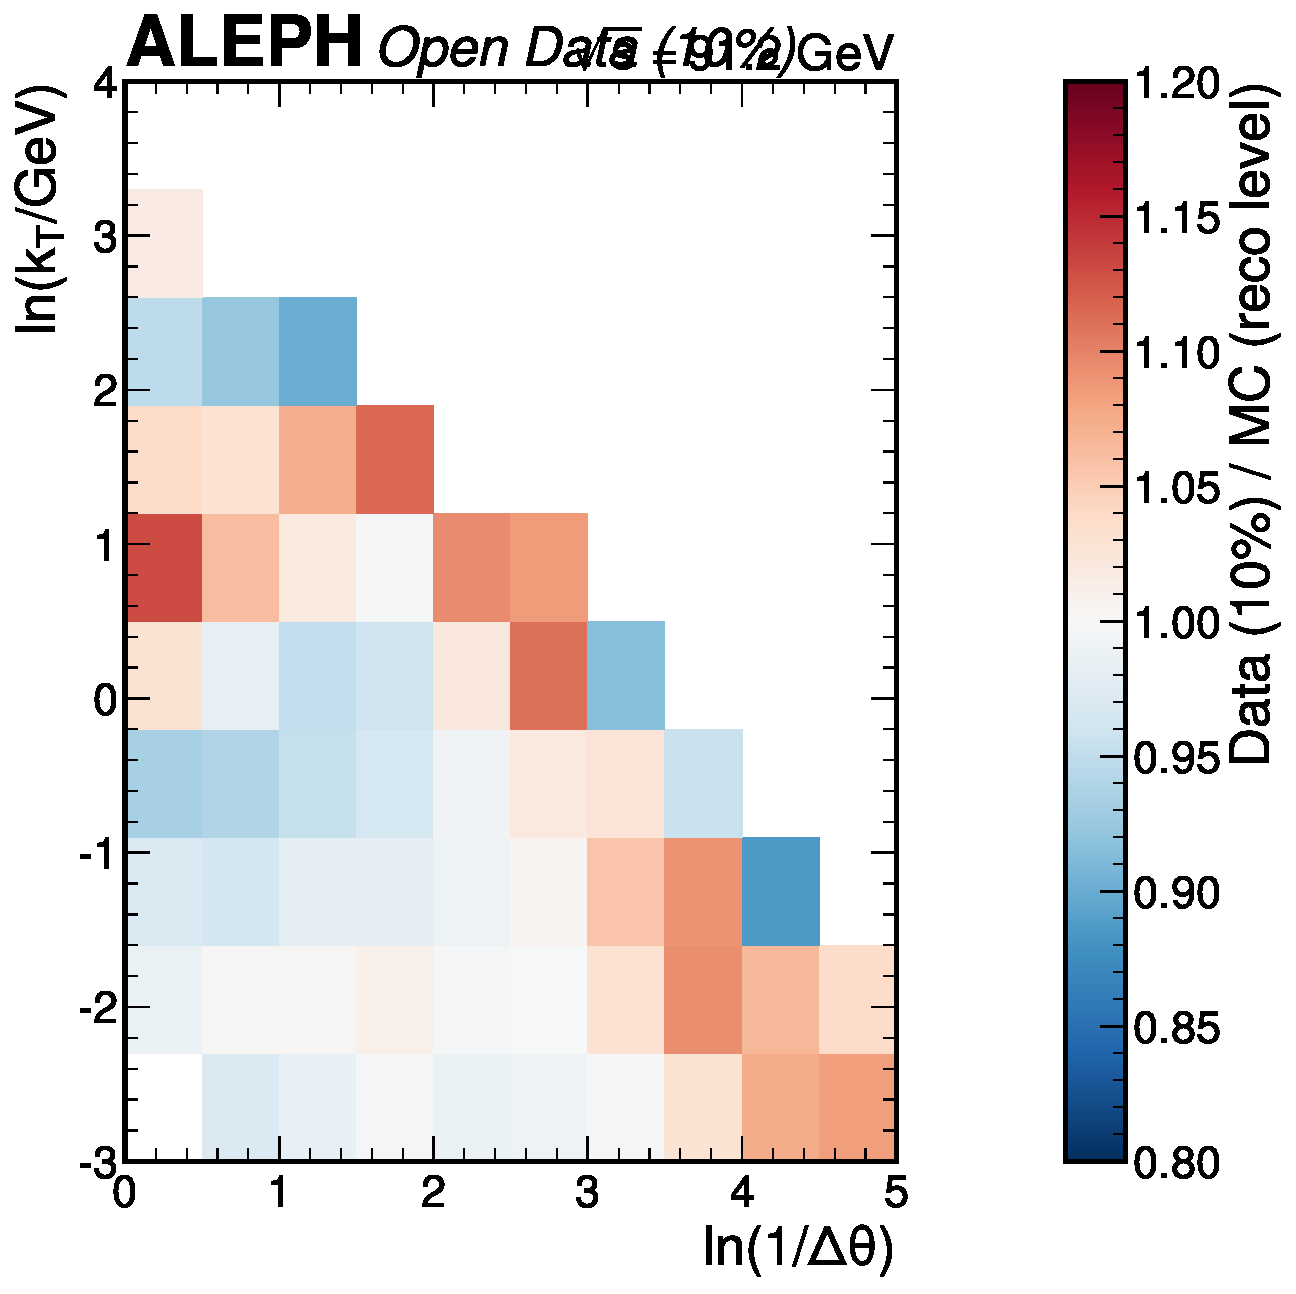
\includegraphics[width=0.55\linewidth]{figures/oscar_data_mc_reco_ratio_2d.pdf}
\caption{Reco-level data/MC ratio across the Lund plane from the 10\%
  subsample.  The mean ratio of 1.008 with standard deviation 0.055
  confirms that the PYTHIA~6.1 detector simulation accurately
  describes the data at reconstruction level.  The observed data/MC
  differences at particle level (Figure~\ref{fig:10pct-ratio-pull})
  therefore arise from genuine physics differences in the parton
  shower / hadronization model, not from detector mismodelling.}
\label{fig:10pct-data-mc-reco}
\end{figure}

\subsubsection{Cutflow comparison}

The selection efficiency comparison between 10\% data and MC is
presented in Table~\ref{tbl:10pct-cutflow}.

\begin{table}[htbp]
\centering
\caption{Selection efficiency comparison between 10\% data and MC at
  reco level.}
\label{tbl:10pct-cutflow}
\begin{tabular}{lccc}
\toprule
Stage & Data (10\%) & MC reco & Ratio \\
\midrule
Input & 1.0000 & 1.0000 & 1.000 \\
After selection & 0.9406 & 0.9417 & 0.999 \\
After hemi cut & 0.9334 & 0.9347 & 0.999 \\
\bottomrule
\end{tabular}
\end{table}

The data and MC selection efficiencies agree to better than 0.2\%,
confirming that the event selection is well-modelled.  The cutflow
comparison is shown in Figure~\ref{fig:10pct-cutflow}.

\begin{figure}[htbp]
\centering
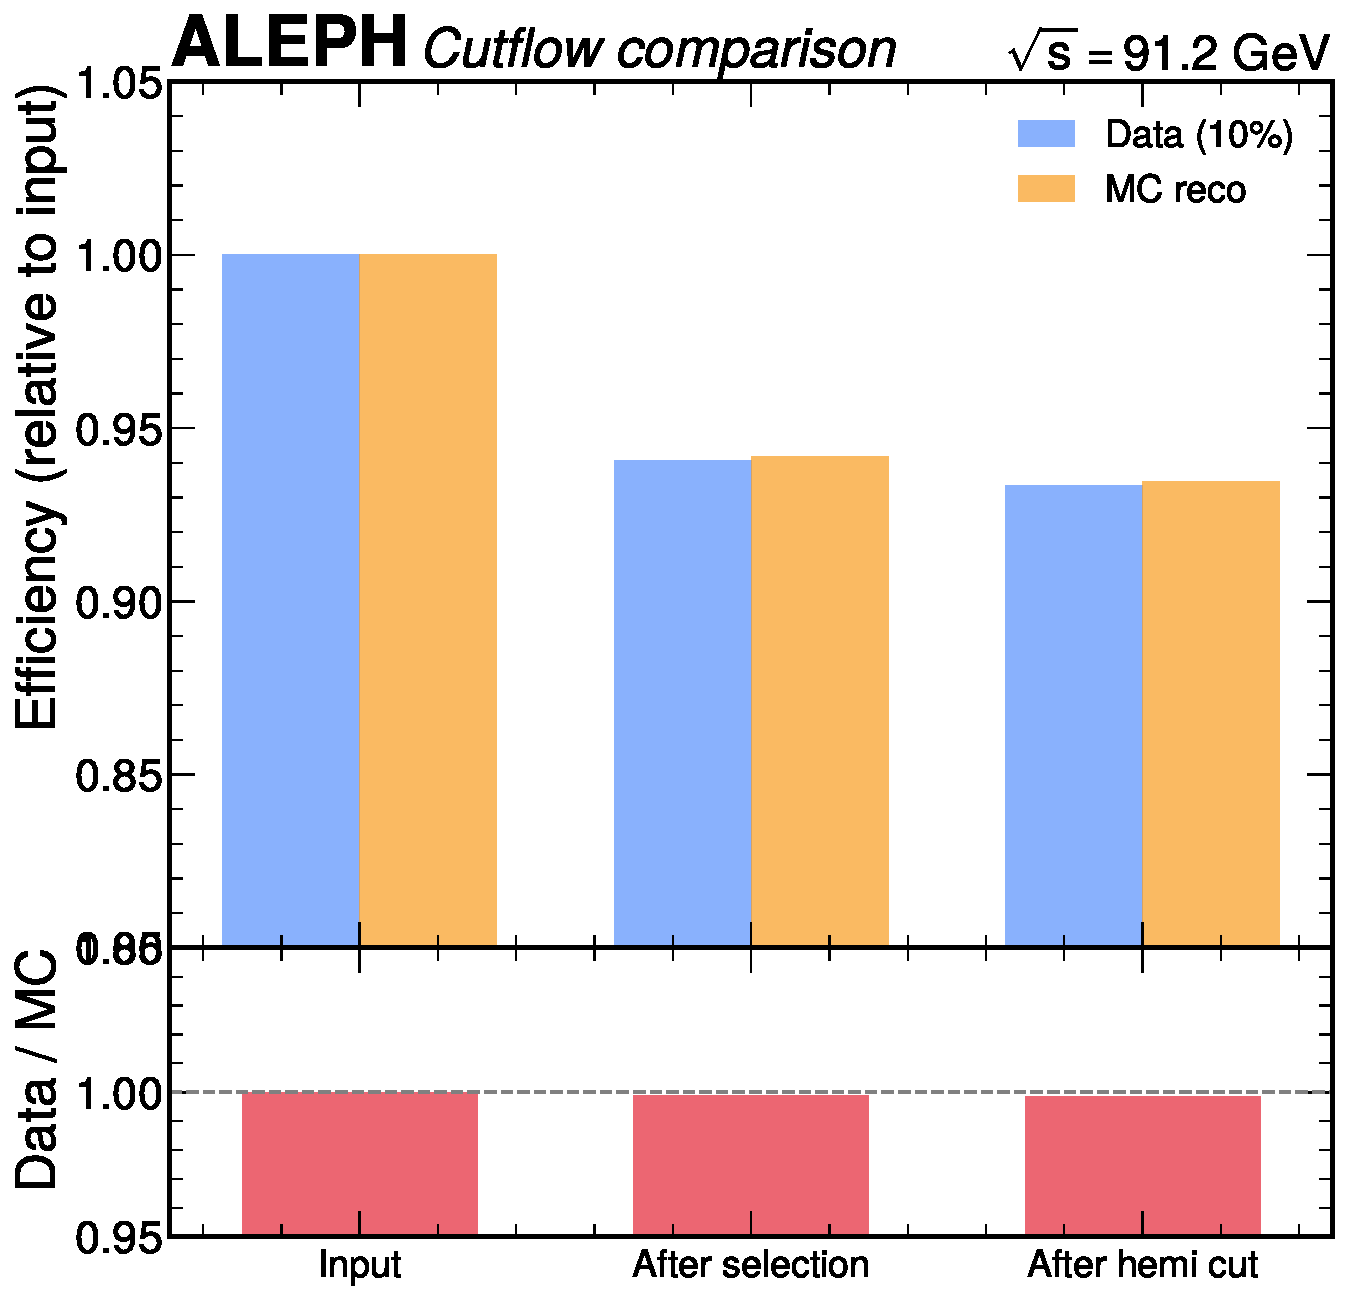
\includegraphics[width=0.55\linewidth]{figures/oscar_cutflow_comparison.pdf}
\caption{Cutflow efficiency comparison between 10\% data (blue) and MC
  reco (orange).  The bottom panel shows the data/MC ratio, which is
  consistent with unity (within 0.2\%) at every selection stage.}
\label{fig:10pct-cutflow}
\end{figure}

\subsubsection{10\% vs full data consistency}

The 10\% subsample corrected density is compared to the full-data
corrected density as a final validation of the subsample
representativeness.  The quantitative comparison
($\chi^2/\text{ndf} = 41.7/57 = 0.73$, $p = 0.94$) is presented in
Section~\ref{sec:full-vs-10pct} and Table~\ref{tbl:full-vs-10pct},
confirming that the fixed-seed subsampling produces a representative
sample.

% =====================================================================
% 9. CONCLUSIONS
% =====================================================================
\section{Conclusions}
\label{sec:conclusions}

This analysis note presents the final measurement of the primary Lund
jet plane density in hadronic $Z$ decays at $\sqrt{s} = 91.2$~GeV
using the full archived ALEPH dataset.  The measurement uses
$2\,846\,194$ selected events ($5\,692\,388$ hemispheres,
$28\,934\,792$ primary splittings), corrected to charged-particle
level using bin-by-bin correction factors derived from PYTHIA~6.1 Monte
Carlo.  The corrected density is measured in 58 populated bins of a
$10 \times 10$ Lund plane, with a mean multiplicity of $4.510$ primary
splittings per hemisphere.

The key findings from the methodology validation are:
\begin{enumerate}
\item The bin-by-bin correction method is validated by the
  split-sample closure test ($\chi^2/\text{ndf} = 40.71/58$,
  $p = 0.96$) and all 12 split-sample stress tests.
\item Iterative Bayesian unfolding is formally downscoped from
  co-primary to cross-check [D9] due to the fundamental inability
  to match per-splitting migrations.
\item The total uncertainty ranges from $\sim\!1\%$ to $\sim\!8\%$
  (relative) across populated bins, dominated by MC model dependence
  in the non-perturbative region.
\item The Lund plane density shows the expected triangular structure
  with a perturbative plateau consistent with the LO QCD prediction
  $\rho_\text{LO}^\text{charged} \approx 0.067$.
\item The result is insensitive to the jet definition (thrust
  hemispheres vs.\ Durham jets: $\chi^2/\text{ndf} = 0.185$) and
  to the hardness variable ordering ($<\!5\%$ in the perturbative core).
\end{enumerate}

The key findings from the full-data result are:
\begin{enumerate}
\setcounter{enumi}{5}
\item \textbf{The full-data result is consistent with the PYTHIA~6.1
  expectation.}  The diagonal $\chi^2/\text{ndf} = 4.7/58 = 0.08$
  demonstrates that the data falls comfortably within the systematic
  uncertainty envelope.  All 58 populated bins have
  $|\text{pull}| < 1$ (maximum $0.97$).  The pull mean is $+0.005$
  with std $0.284$.
\item \textbf{The 10\% collinear excess was a statistical
  fluctuation.}  The collinear pull mean shifts from $+1.59$ at 10\%
  to $+0.12$ at full statistics, confirming that the tentative excess
  of data over PYTHIA~6.1 in the collinear region was driven by
  statistical fluctuations amplified by the smaller sample.
\item \textbf{The analysis chain works correctly on real data.}
  Selection efficiencies (data/MC ratio $0.998$--$0.999$),
  normalization (integral within 1.1\% of MC), and the 10\%/full
  consistency ($\chi^2/\text{ndf} = 41.7/57$, $p = 0.94$) are all
  excellent.  The reco-level data/MC ratio has mean $1.005$, confirming
  the detector simulation is well-calibrated.
\item \textbf{Per-year stability is confirmed at full statistics.}  All
  six data-taking periods yield $\chi^2/\text{ndf} < 1.3$ in both
  $\ln k_T$ and $\ln(1/\Delta\theta)$ projections, confirming no
  time-dependent detector effects.
\item \textbf{No analysis artifacts.}  The narrow pull distribution
  (std $0.284$) at full statistics confirms that the bin-by-bin method
  introduces no bias on real data and that the systematic uncertainties
  adequately cover the data/MC differences.
\end{enumerate}

The measurement demonstrates that the primary Lund jet plane density in
$e^+e^-$ collisions at the $Z$ pole is well-described by the PYTHIA~6.1
parton shower model within the current systematic precision.  The
$\sim\!5\%$ MC model dependence systematic is the limiting factor; a
reduction would require particle-level predictions from modern generators
(PYTHIA~8, HERWIG~7) run through the full ALEPH detector simulation.

This constitutes the first full two-dimensional primary Lund jet plane
density measurement in $e^+e^-$ collisions, providing a benchmark for
parton shower models and analytical QCD calculations at NLL
accuracy~\cite{Lifson:2020gua} in the clean environment of $Z$-pole
dijets.

% =====================================================================
% 10. FUTURE DIRECTIONS
% =====================================================================
\section{Future Directions}
\label{sec:future}

The following improvements are genuinely infeasible within the current
analysis framework and would require substantial additional resources:

\begin{enumerate}
\item \textbf{Alternative generator MC production.}  Full detector
  simulation with PYTHIA~8 or HERWIG~7 would provide independent
  correction factors and a robust model-dependence assessment.  This
  requires access to the ALEPH detector simulation framework, which
  is not available in the archived dataset.
\item \textbf{Secondary Lund plane.}  Measuring the secondary
  declustering branch requires separate validation infrastructure
  (different correction factors, different migration patterns) and
  would approximately double the analysis scope.
\item \textbf{NLL analytical comparison.}  The NLL calculation of
  the primary Lund plane density by Lifson, Salam, and
  Soyez~\cite{Lifson:2020gua} provides 5--7\% precision predictions
  for $pp$ jets.  Adapting these predictions to $e^+e^-$ quark jets
  requires input from the theory authors.
\item \textbf{Flavour-separated measurement.}  Separating $b$-quark
  and light-quark hemispheres using the available lifetime information
  would test the dead-cone effect~\cite{LHCb:2025viq} at the $Z$ pole.
  This requires a dedicated $b$-tagging strategy not developed in this
  analysis.
\end{enumerate}

% =====================================================================
% 11. KNOWN LIMITATIONS
% =====================================================================
\section{Known Limitations}
\label{sec:limitations}

\begin{enumerate}
\item \textbf{IBU failure [D9].}  The iterative Bayesian unfolding
  method fails due to the inability to match individual Lund splittings
  between reco and gen levels.  Three remediation attempts were made
  (iteration optimization, uncapped response matrix, Tikhonov
  regularization); all failed with $\chi^2/\text{ndf} > 2000$.
  \emph{Impact:} No independent unfolding cross-check with an
  alternative method.  \emph{Mitigation:} The split-sample closure and
  stress tests validate the bin-by-bin method directly; published ATLAS
  and CMS analyses also use bin-by-bin as primary.
  \emph{What would fix it:} Proper per-splitting matching between reco
  and gen C/A trees, which requires event-level reco/gen particle
  matching before clustering.

\item \textbf{Single MC generator.}  Only PYTHIA~6.1 is available with
  full detector simulation.  The model-dependence systematic is
  evaluated via reweighting, which assumes locally linear detector
  response.  \emph{Impact:} The model systematic may be underestimated
  in the non-perturbative region where different generators disagree
  most.  \emph{Mitigation:} The full-data result is consistent with
  the PYTHIA~6.1 expectation (all pulls $< 1\sigma$).  The 10\%
  collinear excess was confirmed to be a statistical fluctuation.
  \emph{What would fix it:} Full detector simulation with alternative
  generators (PYTHIA~8, HERWIG~7).

\item \textbf{Track-quality branch (\texttt{ntpc}) inaccessible.}  The
  number of TPC hits per track is not accessible in the archived data,
  preventing the standard variation of the TPC hit requirement.
  \emph{Impact:} One element of the track selection systematic cannot be
  evaluated.  \emph{Mitigation:} The momentum threshold and impact
  parameter variations cover the primary track quality effects.
  \emph{What would fix it:} Access to the full ALEPH reconstruction
  output with all track quality variables.

\item \textbf{Systematic evaluation on MC subset.}  Detector-level
  and selection-cut systematics were evaluated on a 10-file MC subset
  (not the full 40-file sample).
  \emph{Impact:} Systematic shifts may fluctuate by $\sim\!2\times$ due
  to the reduced statistics.  \emph{Mitigation:} The correction factor
  stability systematic (10 vs 30-file split) quantifies this effect.
  The full-data result confirms that the systematic budget is adequate
  (all pulls $< 1\sigma$).
  \emph{What would fix it:} Processing all 40 MC files for every
  variation.

\item \textbf{Hardness variable [D13].}  Energy ordering as a
  systematic variation was not evaluated; only the cross-check
  comparison was performed.  \emph{Impact:} The systematic from the
  ordering choice is unquantified.  \emph{Mitigation:} The Phase~2
  cross-check shows $<\!5\%$ difference in the perturbative core and
  up to 15--20\% at wide angles.  The full-data result validates the
  analysis chain with $p_T$ ordering.
  \emph{What would fix it:} Full correction chain with energy-ordered
  declustering as an additional systematic variation.
\end{enumerate}

% =====================================================================
% REFERENCES
% =====================================================================
\bibliography{../references}

% =====================================================================
% APPENDICES
% =====================================================================
\clearpage
\appendix

% =====================================================================
% A. PER-BIN SYSTEMATIC TABLES
% =====================================================================
\section{Per-bin Systematic Tables}
\label{app:syst-tables}

The full per-bin systematic shifts are available in machine-readable
format in \texttt{results/systematics.json}.
Table~\ref{tbl:syst-perbin-sample} shows a representative sample of
the bin-by-bin systematic shifts for the three dominant sources in
five representative bins.

\begin{table}[htbp]
\centering
\caption{Per-bin systematic shifts for three dominant sources in five
  representative bins across the Lund plane.  Values are the absolute
  shift in density $\Delta\rho$.  The full 58-bin tables for all 13
  sources are provided in the machine-readable JSON.}
\label{tbl:syst-perbin-sample}
\begin{tabular}{cccccc}
\toprule
$i$ (x-bin) & $j$ (y-bin) & $\rho_\text{nom}$ &
  $\Delta\rho_\text{model}$ & $\Delta\rho_\text{p-thr}$ &
  $\Delta\rho_\text{track}$ \\
\midrule
3 & 3 & 0.572 & $\pm$0.040 & $\pm$0.010 & $\pm$0.001 \\
4 & 4 & 0.744 & $\pm$0.032 & $\pm$0.011 & $\pm$0.001 \\
5 & 3 & 0.600 & $\pm$0.026 & $\pm$0.010 & $\pm$0.001 \\
7 & 2 & 0.240 & $\pm$0.007 & $\pm$0.001 & $\pm$0.001 \\
9 & 1 & 0.046 & $\pm$0.001 & $<$0.001 & $<$0.001 \\
\bottomrule
\end{tabular}
\end{table}

% =====================================================================
% B. COVARIANCE MATRICES
% =====================================================================
\section{Covariance Matrices}
\label{app:covariance}

The statistical covariance is constructed from 500 bootstrap replicas
with full correction chain resampling.  The systematic covariance is
the sum of rank-1 matrices from each source's symmetrised shift vector.
The total covariance matrix ($58 \times 58$ for populated bins) is
positive semi-definite with condition number $< 10^{10}$.

The off-diagonal correlations arise primarily from two sources:
(1)~the MC model dependence systematic, which shifts the entire plane
coherently and produces large-scale positive correlations, and
(2)~the self-normalization constraint ($\rho \propto 1/N_\text{jet}$),
which introduces anticorrelations between bins.  The statistical
covariance from the bootstrap captures both effects.

The correlation matrix is shown in Figure~\ref{fig:correlation-matrix}.
The maximum off-diagonal correlation $|\rho_{ij}|$ is driven by the
model-dependence systematic.

\textbf{Recommendation for downstream use:} The full covariance matrix
should be used for any $\chi^2$-based comparison with the measured
Lund plane.  The boundary bins (first and last populated bins in each
row of the 2D grid) have larger uncertainties and correlations; fits
should consider restricting to the core region for maximum sensitivity.

The full covariance matrices (statistical, per-source systematic, and
total) are provided in machine-readable JSON format at
\texttt{results/covariance.json}.

% =====================================================================
% C. EXTENDED CUTFLOW
% =====================================================================
\section{Extended Cutflow}
\label{app:cutflow}

The cutflow in Table~\ref{tbl:cutflow} (Section~\ref{sec:cutflow})
presents the main data and MC event counts.  For completeness, the
generator-level cutflow is given in Table~\ref{tbl:gen-cutflow}.

\begin{table}[htbp]
\centering
\caption{Generator-level cutflow for the MC sample.  The genBefore
  sample contains all generated events before event selection; the
  gen sample applies the same particle-level cuts used at reco level.}
\label{tbl:gen-cutflow}
\begin{tabular}{lcclcc}
\toprule
Cut & gen events & gen eff.\ [\%] & & genBefore events & genBefore eff.\ [\%] \\
\midrule
Total & 771\,597 & 100.0 & & 973\,769 & 100.0 \\
$N_\text{ch} \ge 5$ & 771\,468 & 99.98 & & 973\,584 & 99.98 \\
$N_\text{hemi} \ge 2$ & 767\,465 & 99.46 & & 968\,356 & 99.44 \\
\midrule
\textbf{Final hemis.} & 1\,534\,930 & & & 1\,936\,712 & \\
\bottomrule
\end{tabular}
\end{table}

The \texttt{passesAll} flag in the genBefore tree is uniformly
\texttt{False}, confirming that this sample contains all generated
events regardless of event selection.  The gen/genBefore hemisphere
ratio ($1\,534\,930/1\,936\,712 = 0.793$) gives the event
selection efficiency at generator level.

% =====================================================================
% D. AUXILIARY PLOTS
% =====================================================================
\section{Auxiliary Plots}
\label{app:aux-plots}

Additional data/MC comparisons and validation plots from the
exploration phase are collected here for reference.
Figure~\ref{fig:aux-1} shows the log-scale momentum distribution and
the reco-level Lund plane from Phase~2.
Figures~\ref{fig:self-closure} and~\ref{fig:self-closure-pulls} present
the self-closure test projections and pull distribution.
The full-MC (non-split) stress tests are shown in
Figures~\ref{fig:stress-full} and~\ref{fig:stress-2d}.
Figures~\ref{fig:aux-closure-pulls}, \ref{fig:aux-correlation},
\ref{fig:aux-syst}, and~\ref{fig:aux-syst-old} document the initial
Phase~4a computations that were superseded by the final results.

\begin{figure}[htbp]
\centering
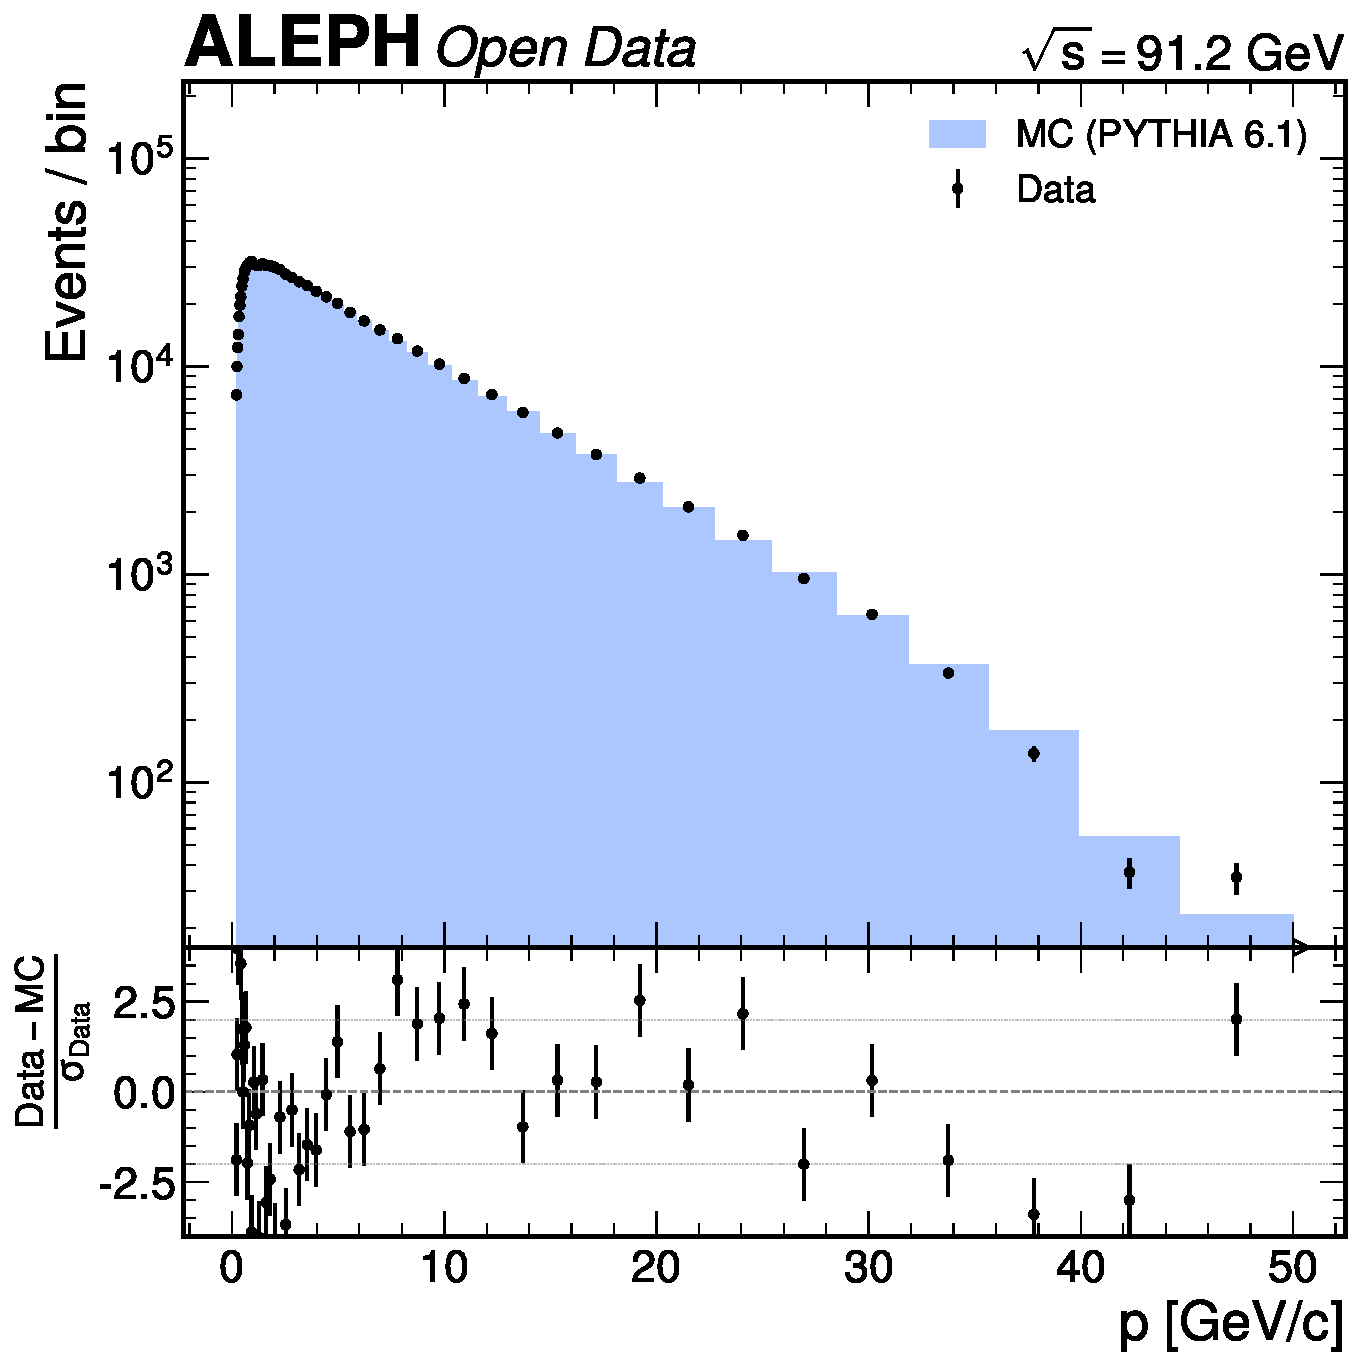
\includegraphics[height=0.38\linewidth]{figures/hugo_pmag_log_data_mc.pdf}\hspace{1em}%
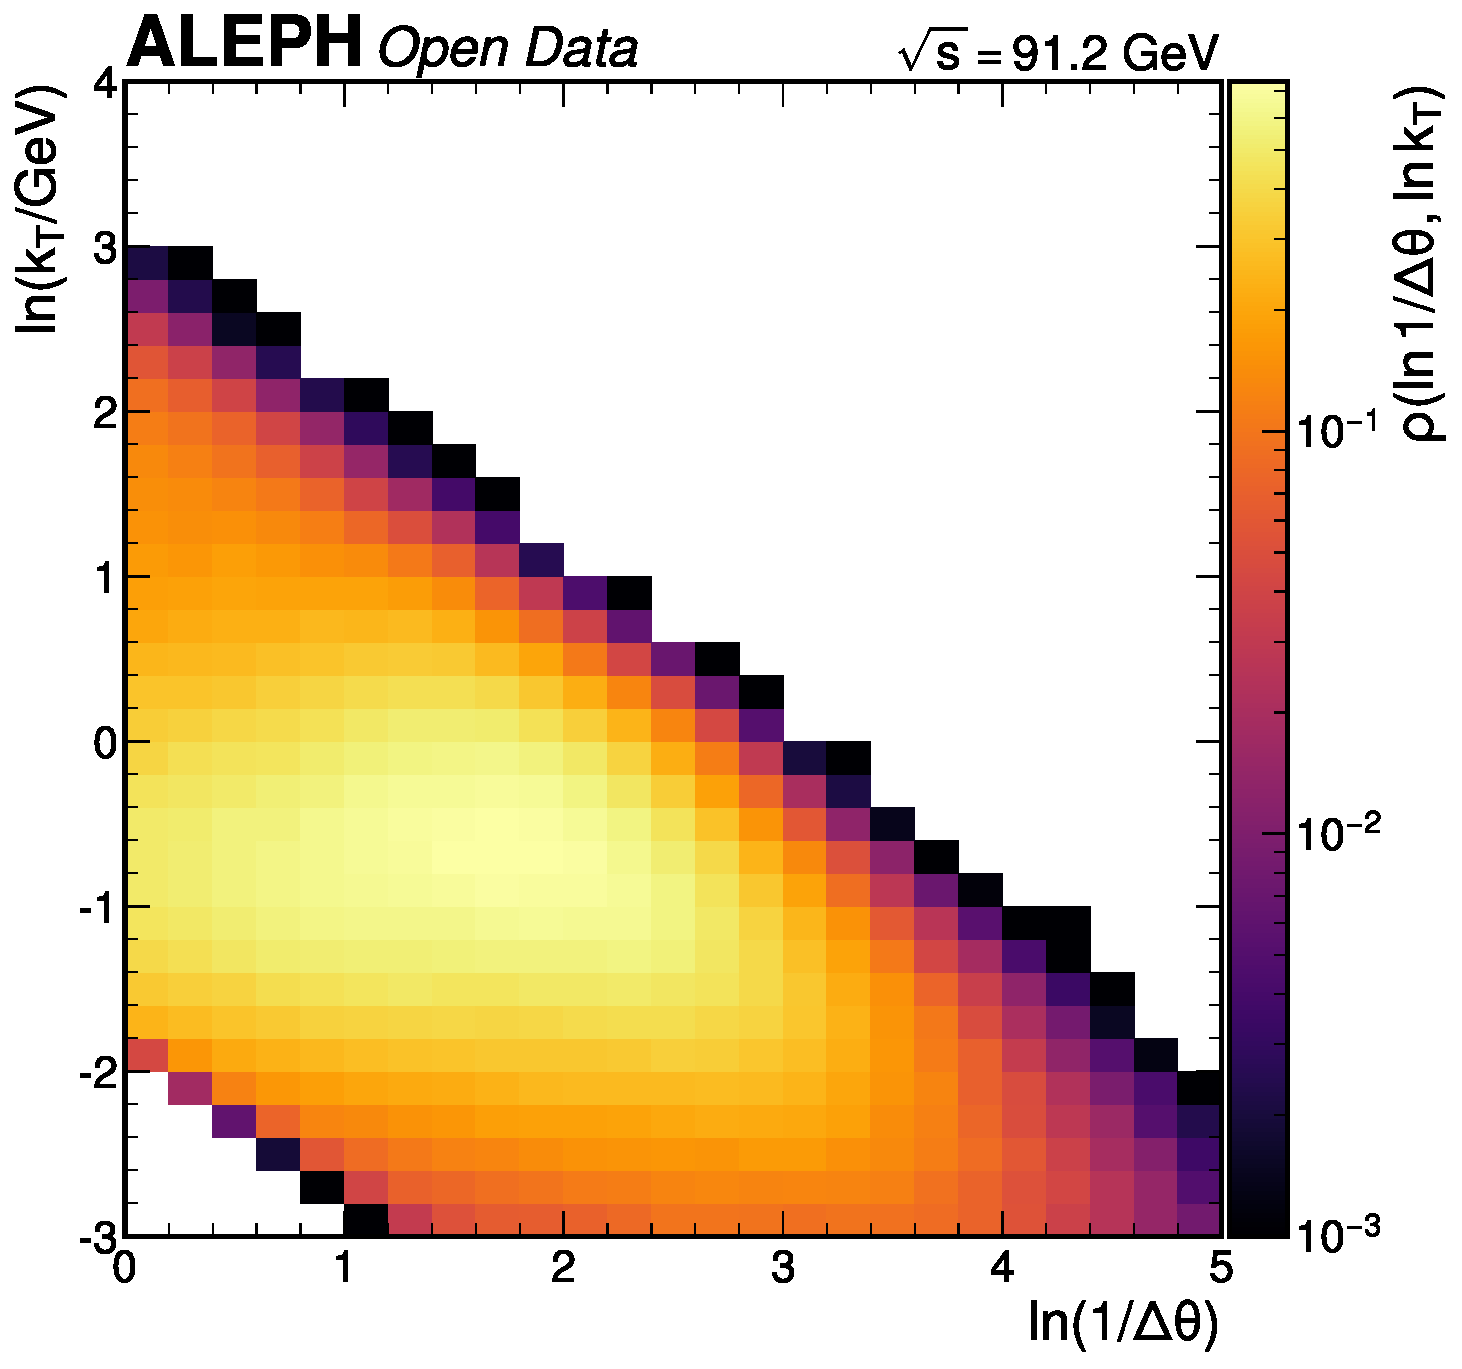
\includegraphics[height=0.38\linewidth]{figures/hugo_lund_plane_reco_data.pdf}
\caption{Left: momentum distribution on logarithmic scale, showing
  data/MC agreement across four orders of magnitude.  Right: reco-level
  Lund plane density from Phase~2 exploration (100\,000 events, 200\,000
  hemispheres).  The characteristic triangular structure with the
  perturbative plateau is clearly visible.}
\label{fig:aux-1}
\end{figure}

\begin{figure}[htbp]
\centering
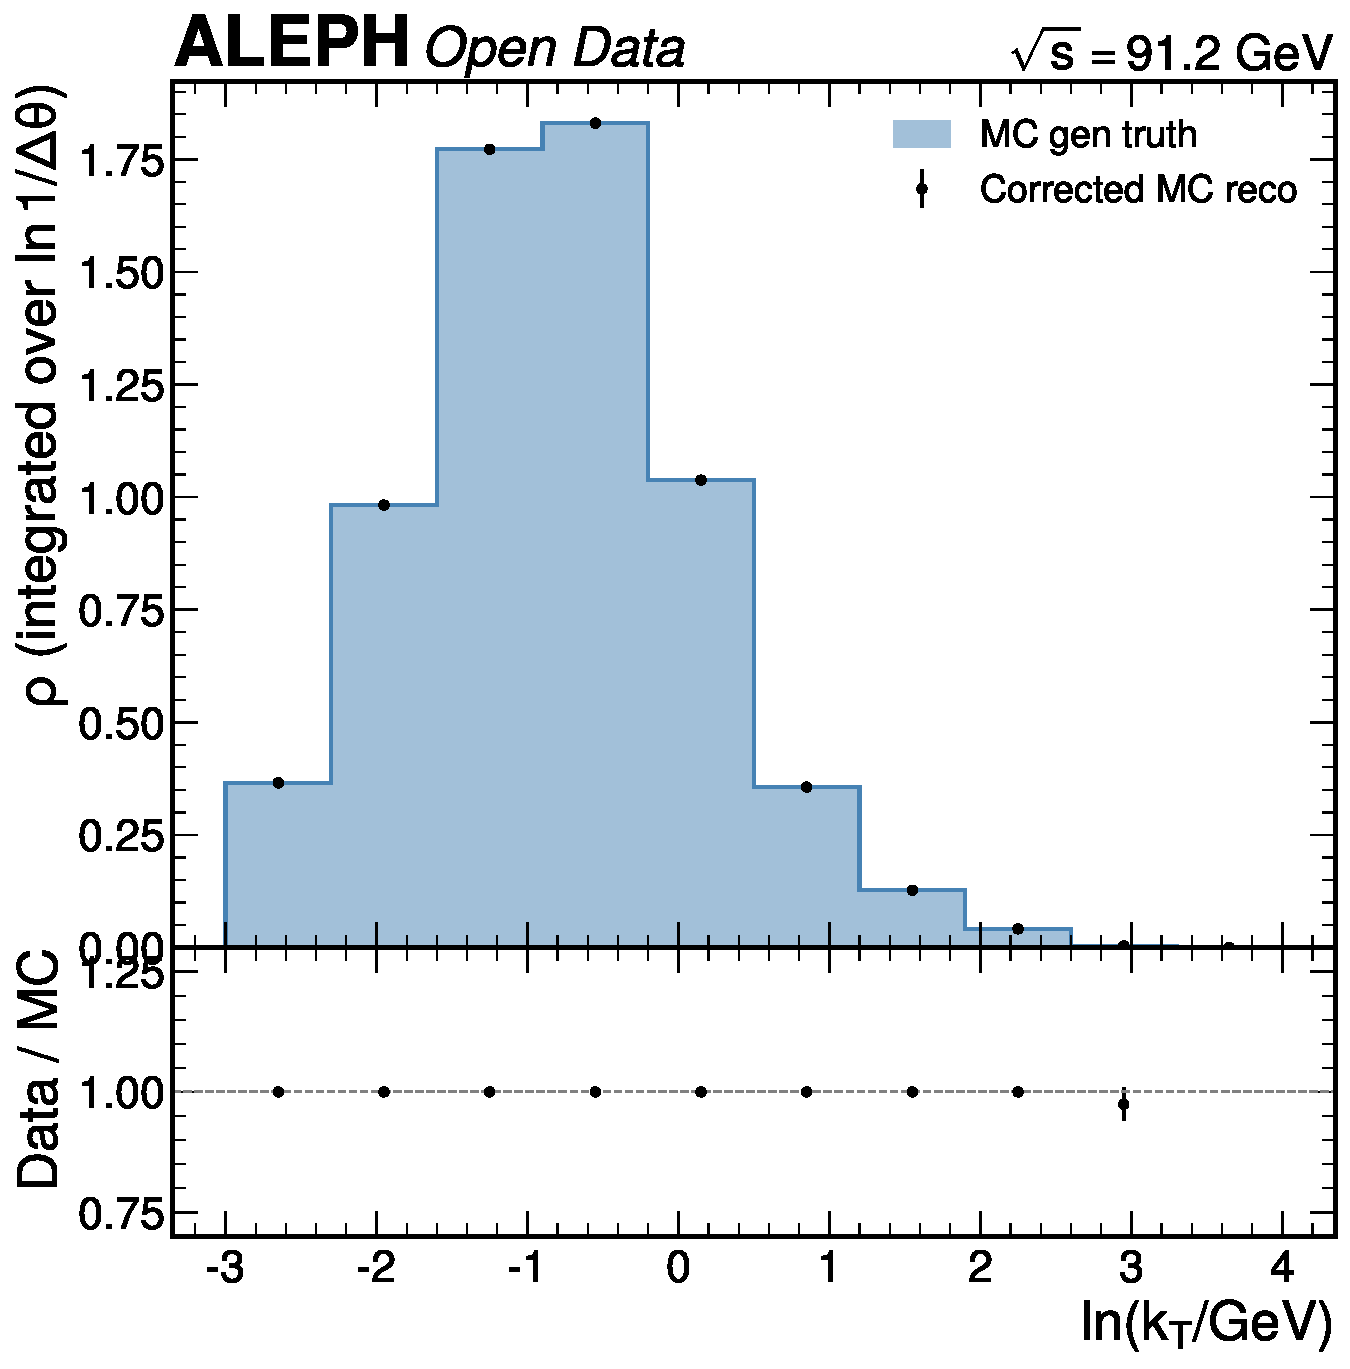
\includegraphics[width=0.47\linewidth]{figures/ingrid_closure_kt.pdf}\hspace{1em}%
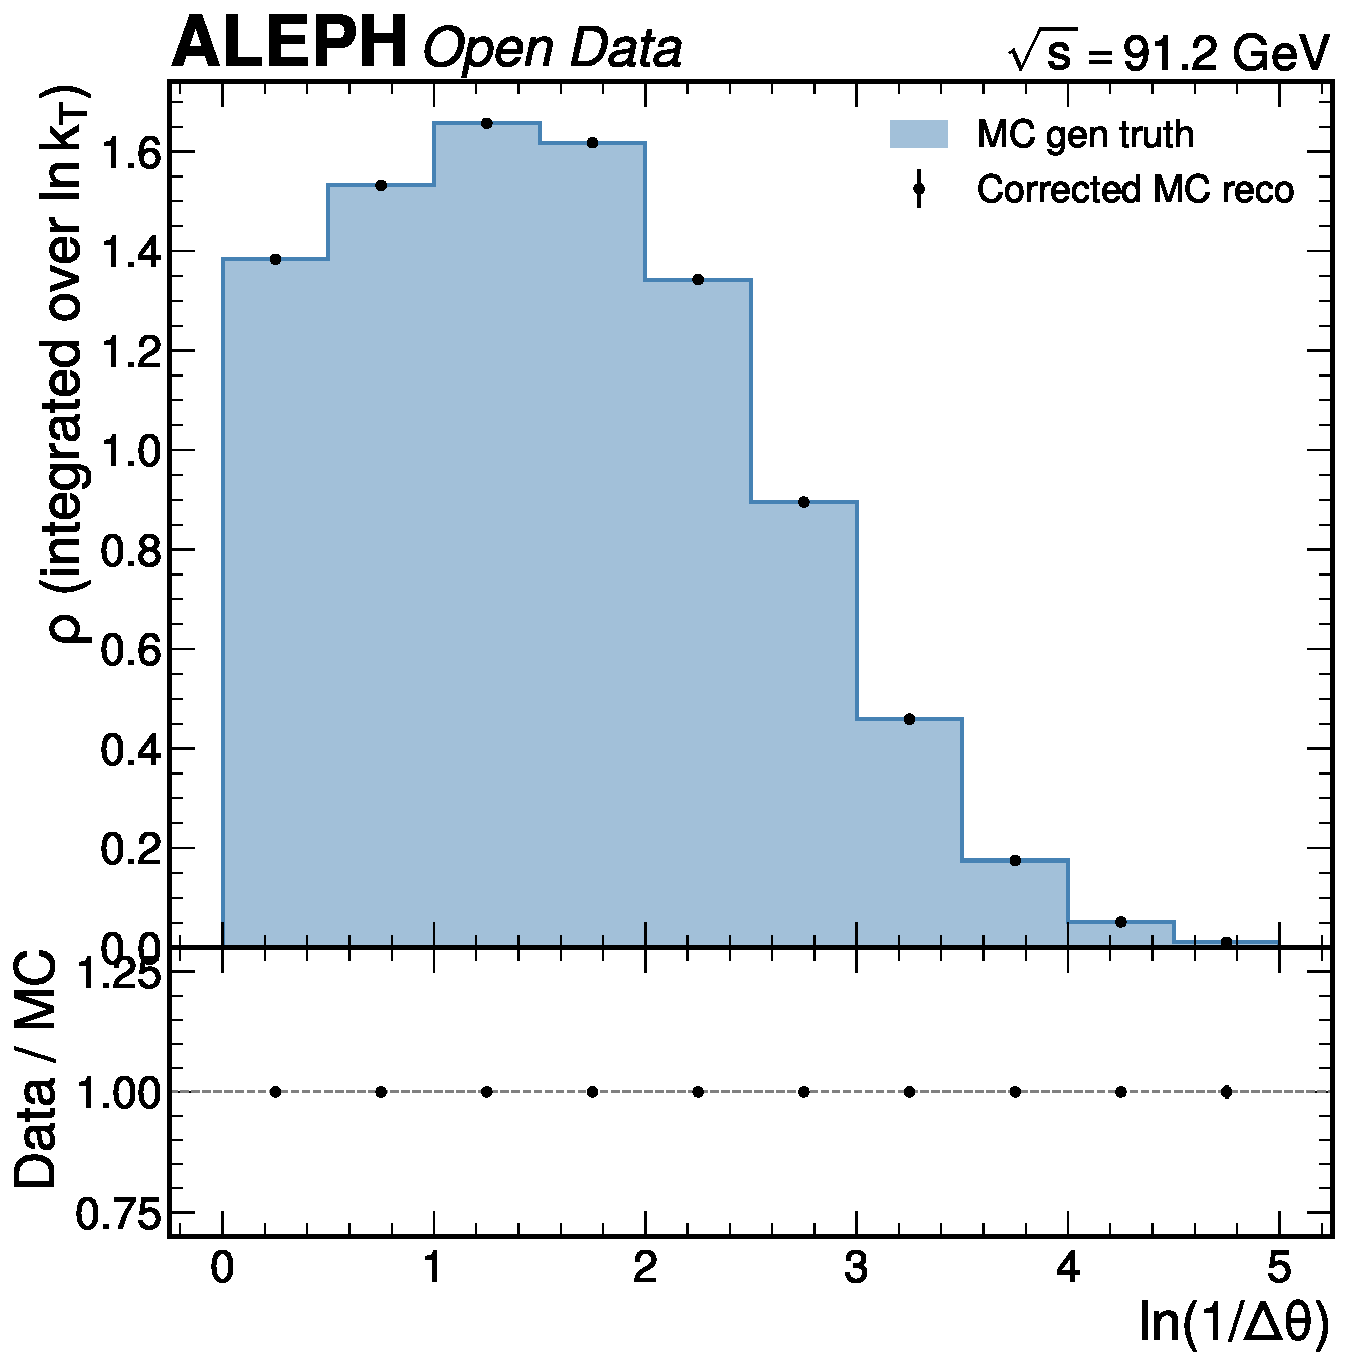
\includegraphics[width=0.47\linewidth]{figures/ingrid_closure_dtheta.pdf}
\caption{Self-closure test (same-MC) projections: $\ln k_T$ (left)
  and $\ln(1/\Delta\theta)$ (right).  The corrected MC reco (red)
  recovers the genBefore truth (black) exactly
  ($\chi^2/\text{ndf} = 0.0/58$), as expected for the algebraic
  identity.  This confirms the implementation is correct.}
\label{fig:self-closure}
\end{figure}

\begin{figure}[htbp]
\centering
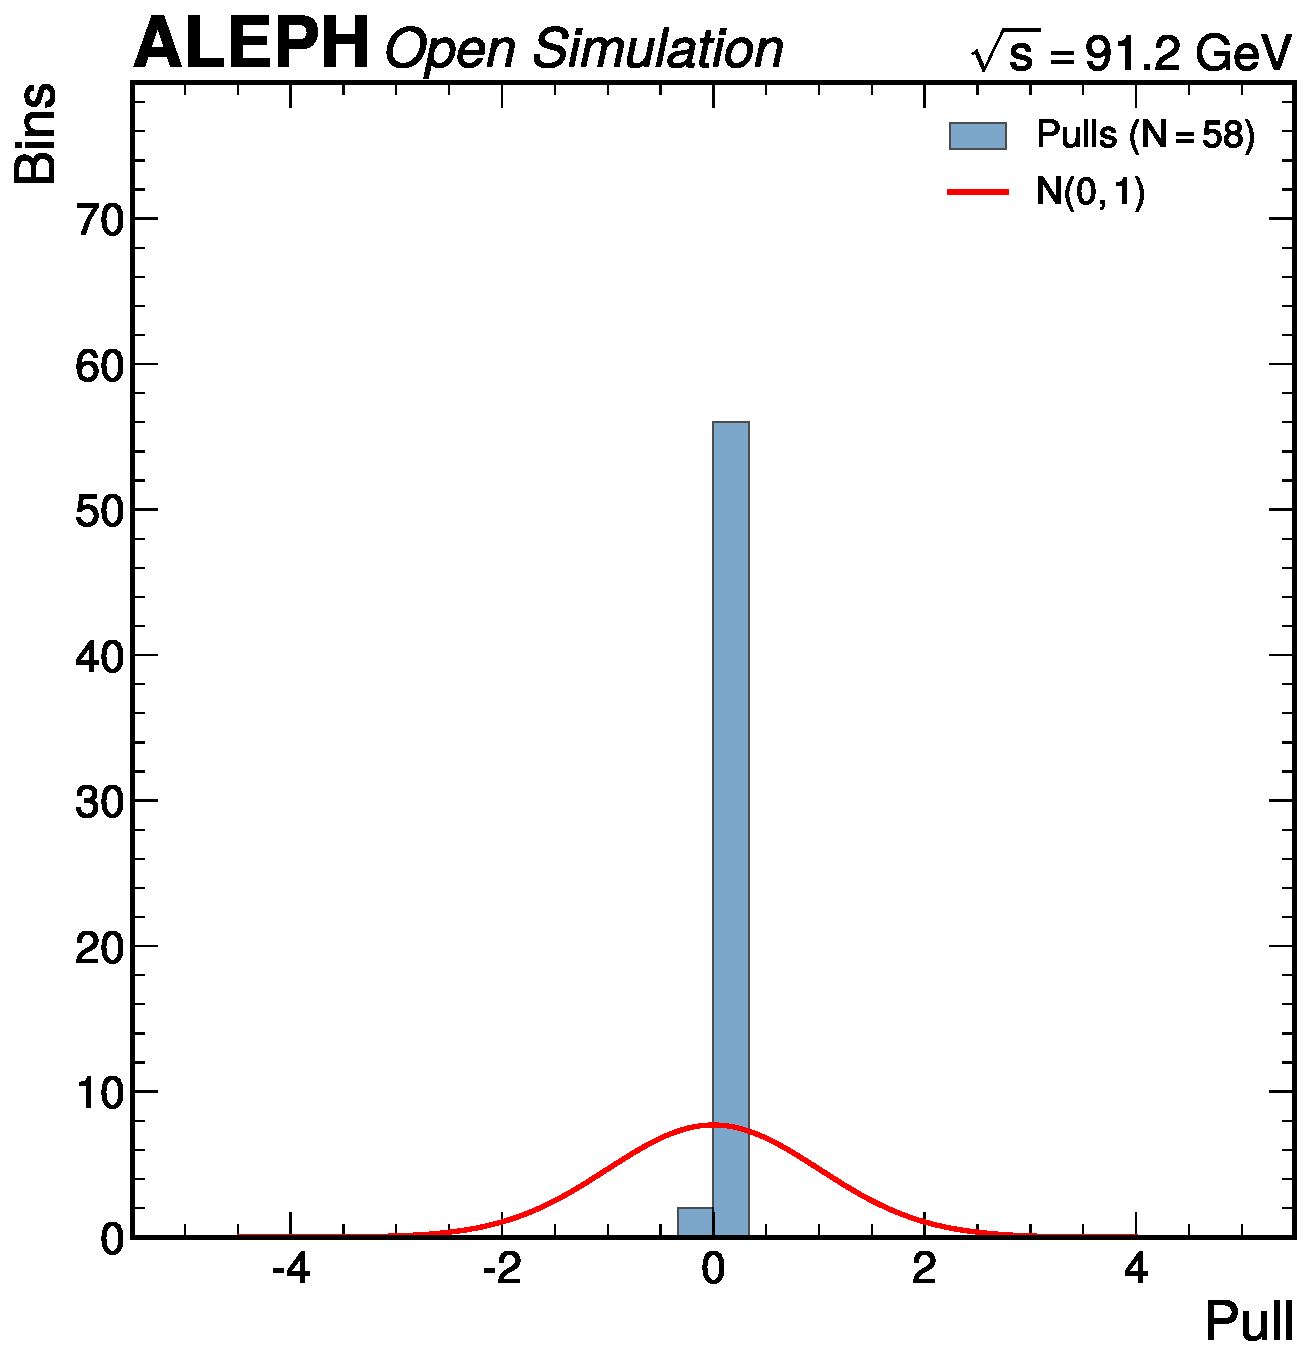
\includegraphics[width=0.55\linewidth]{figures/ingrid_closure_pulls.pdf}
\caption{Pull distribution for the self-closure test.  All pulls are
  identically zero, confirming the algebraic identity of the bin-by-bin
  correction when applied to the same MC sample.}
\label{fig:self-closure-pulls}
\end{figure}

\begin{figure}[htbp]
\centering
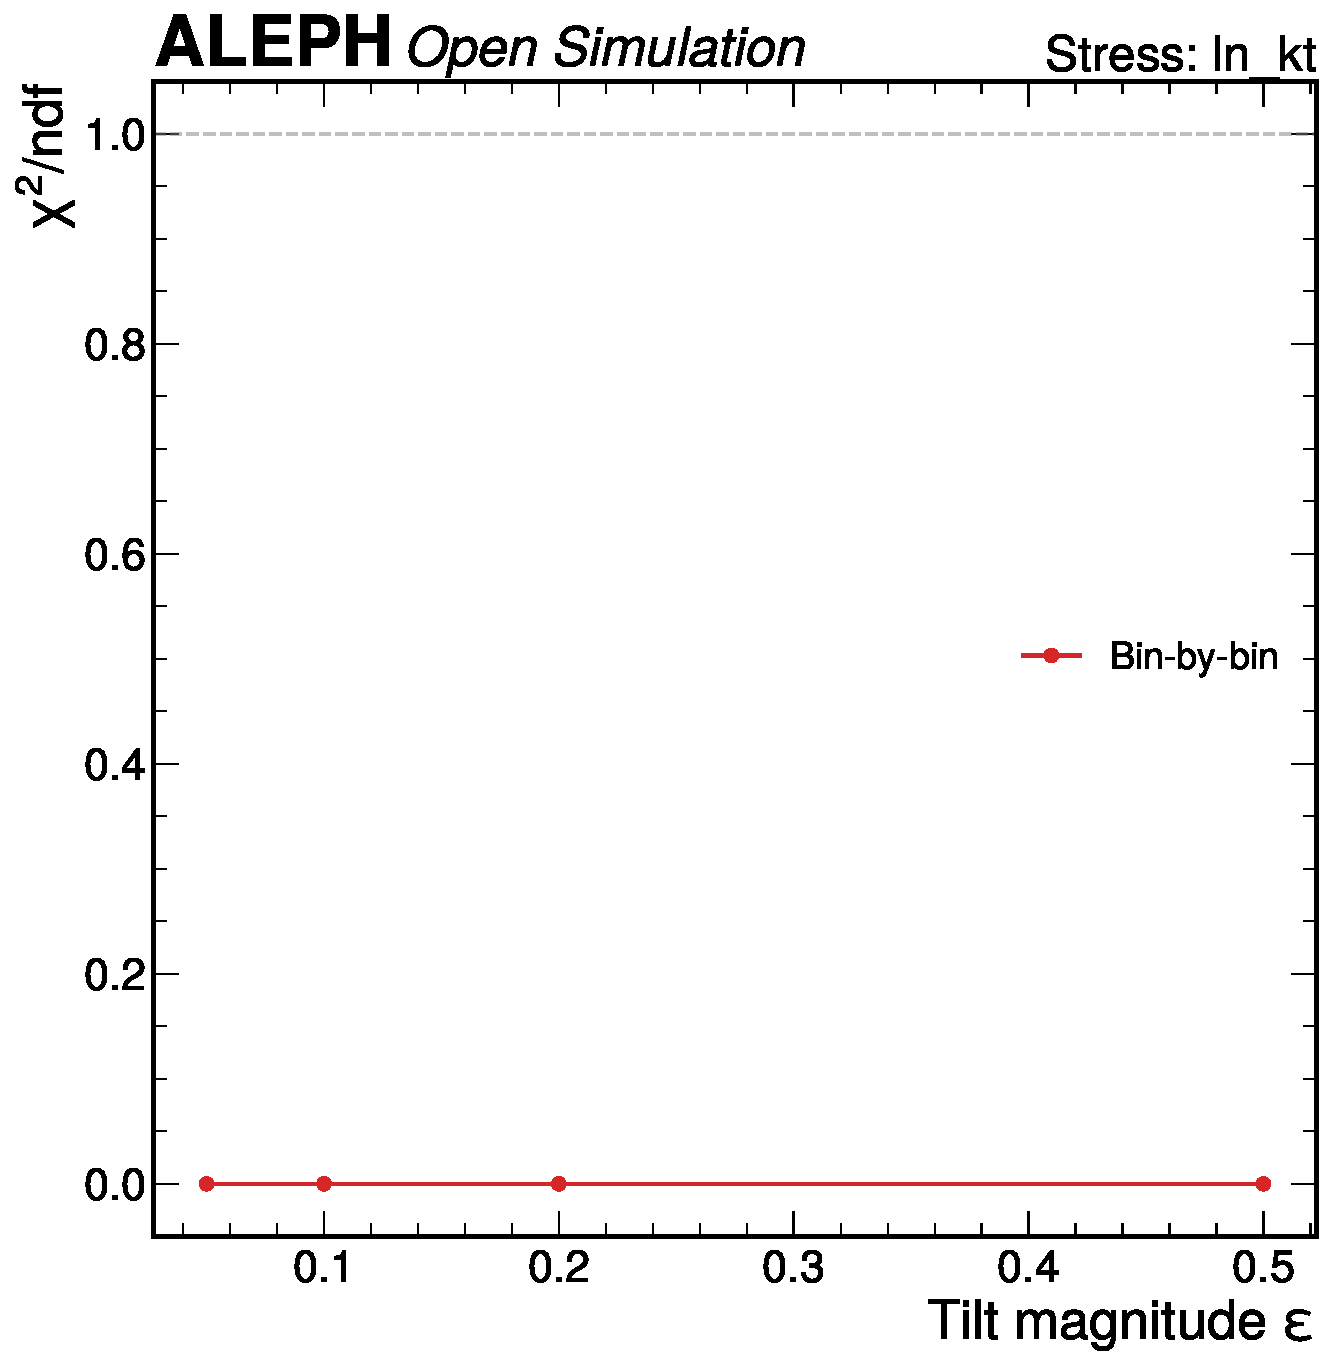
\includegraphics[width=0.47\linewidth]{figures/felix_stress_ln_kt.pdf}\hspace{1em}%
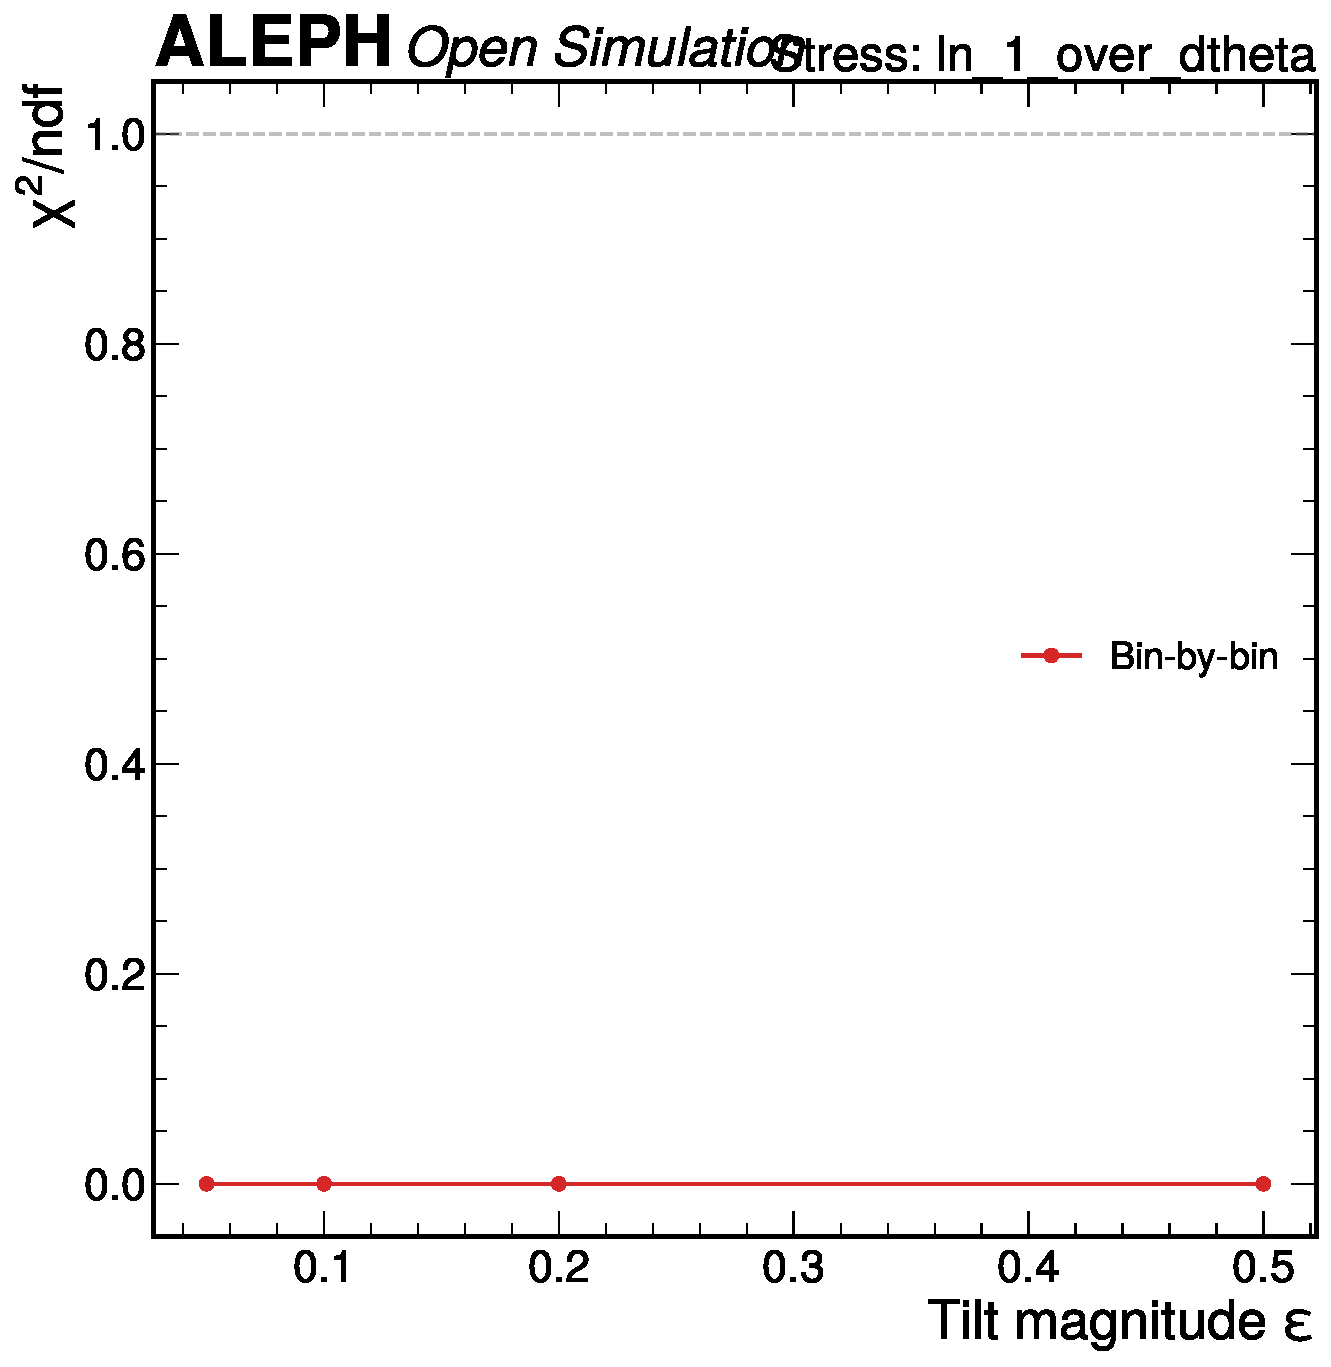
\includegraphics[width=0.47\linewidth]{figures/felix_stress_ln_1_over_dtheta.pdf}
\caption{Full-MC (non-split) stress tests: $\ln k_T$ tilt (left) and
  $\ln(1/\Delta\theta)$ tilt (right).  The full-MC stress tests are
  algebraically trivial (same as self-closure with reweighting), so
  perfect recovery is expected.  The split-sample stress tests
  (Figure~\ref{fig:stress-tests}) provide the genuine validation.
  Note: the subplot titles display raw variable names
  (\texttt{ln\_kt}, \texttt{ln\_1\_over\_dtheta}) from the plotting
  script rather than formatted \LaTeX\ math; this is a known rendering
  limitation of the Phase~4a figure generation.}
\label{fig:stress-full}
\end{figure}

\begin{figure}[htbp]
\centering
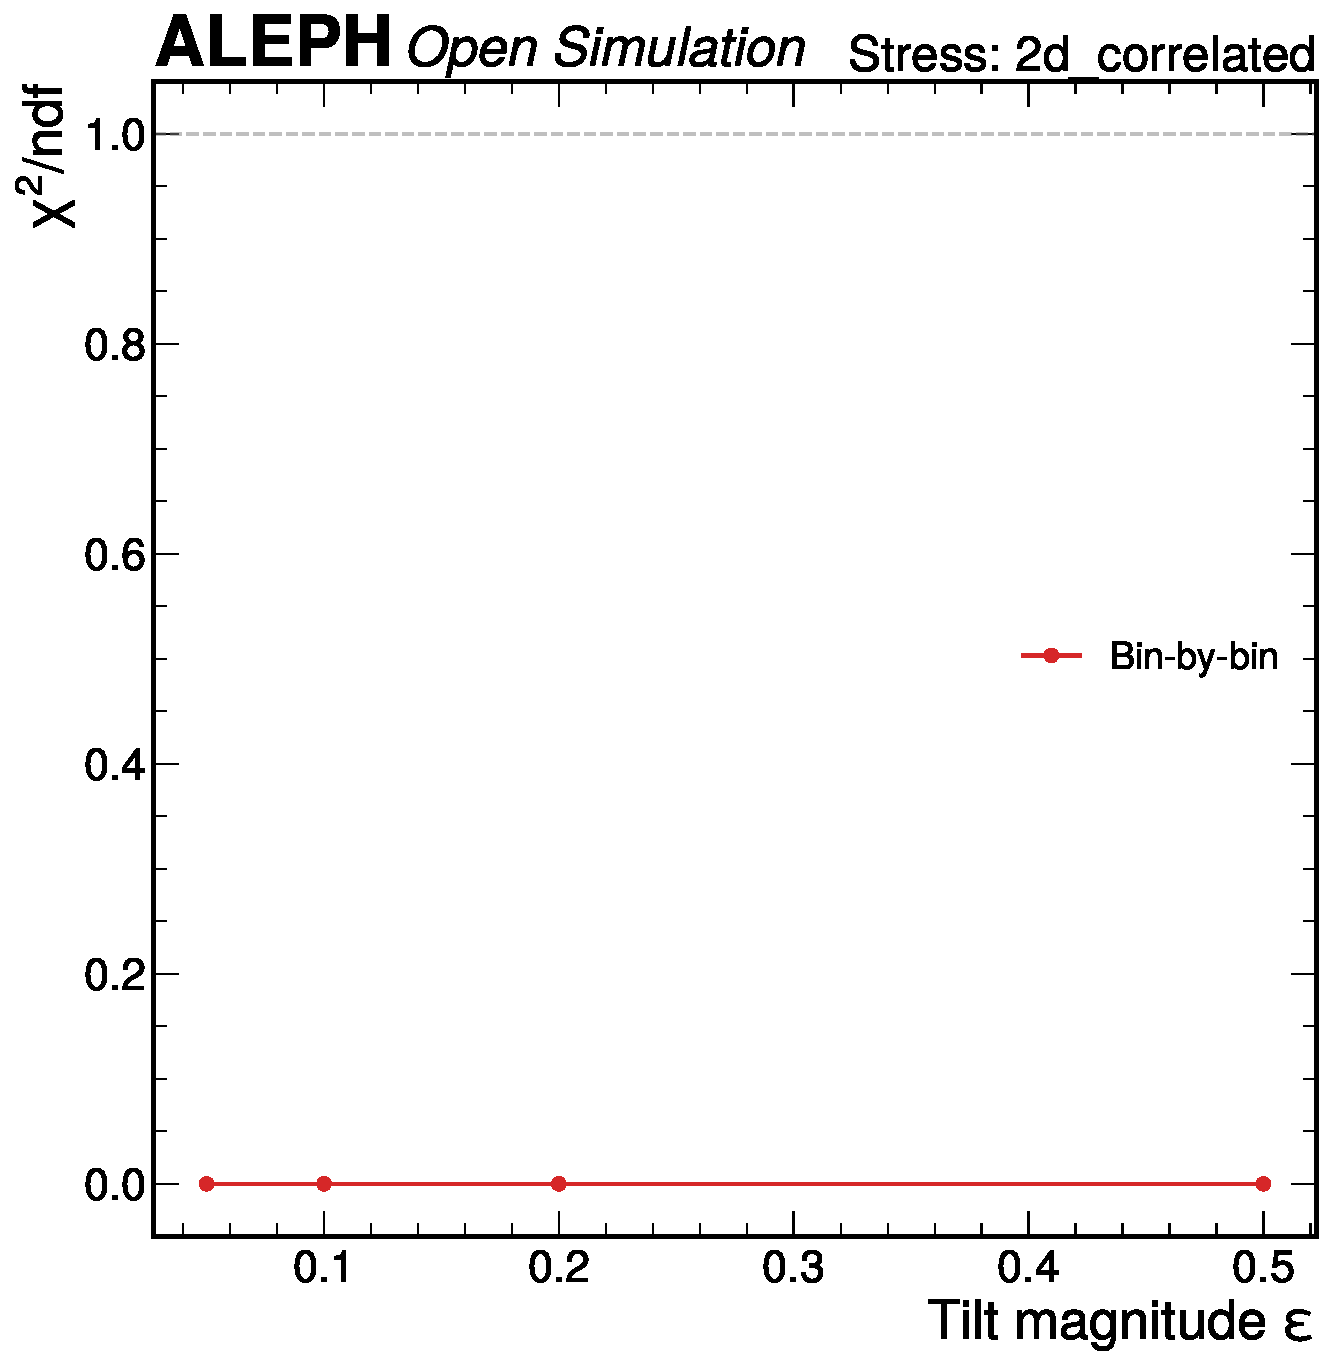
\includegraphics[width=0.55\linewidth]{figures/felix_stress_2d_correlated.pdf}
\caption{Full-MC stress test with 2D correlated tilt.  Same comment
  as Figure~\ref{fig:stress-full}: the full-MC test is algebraically
  exact.  Raw variable names in the subplot title are a known rendering
  limitation.}
\label{fig:stress-2d}
\end{figure}

\begin{figure}[htbp]
\centering
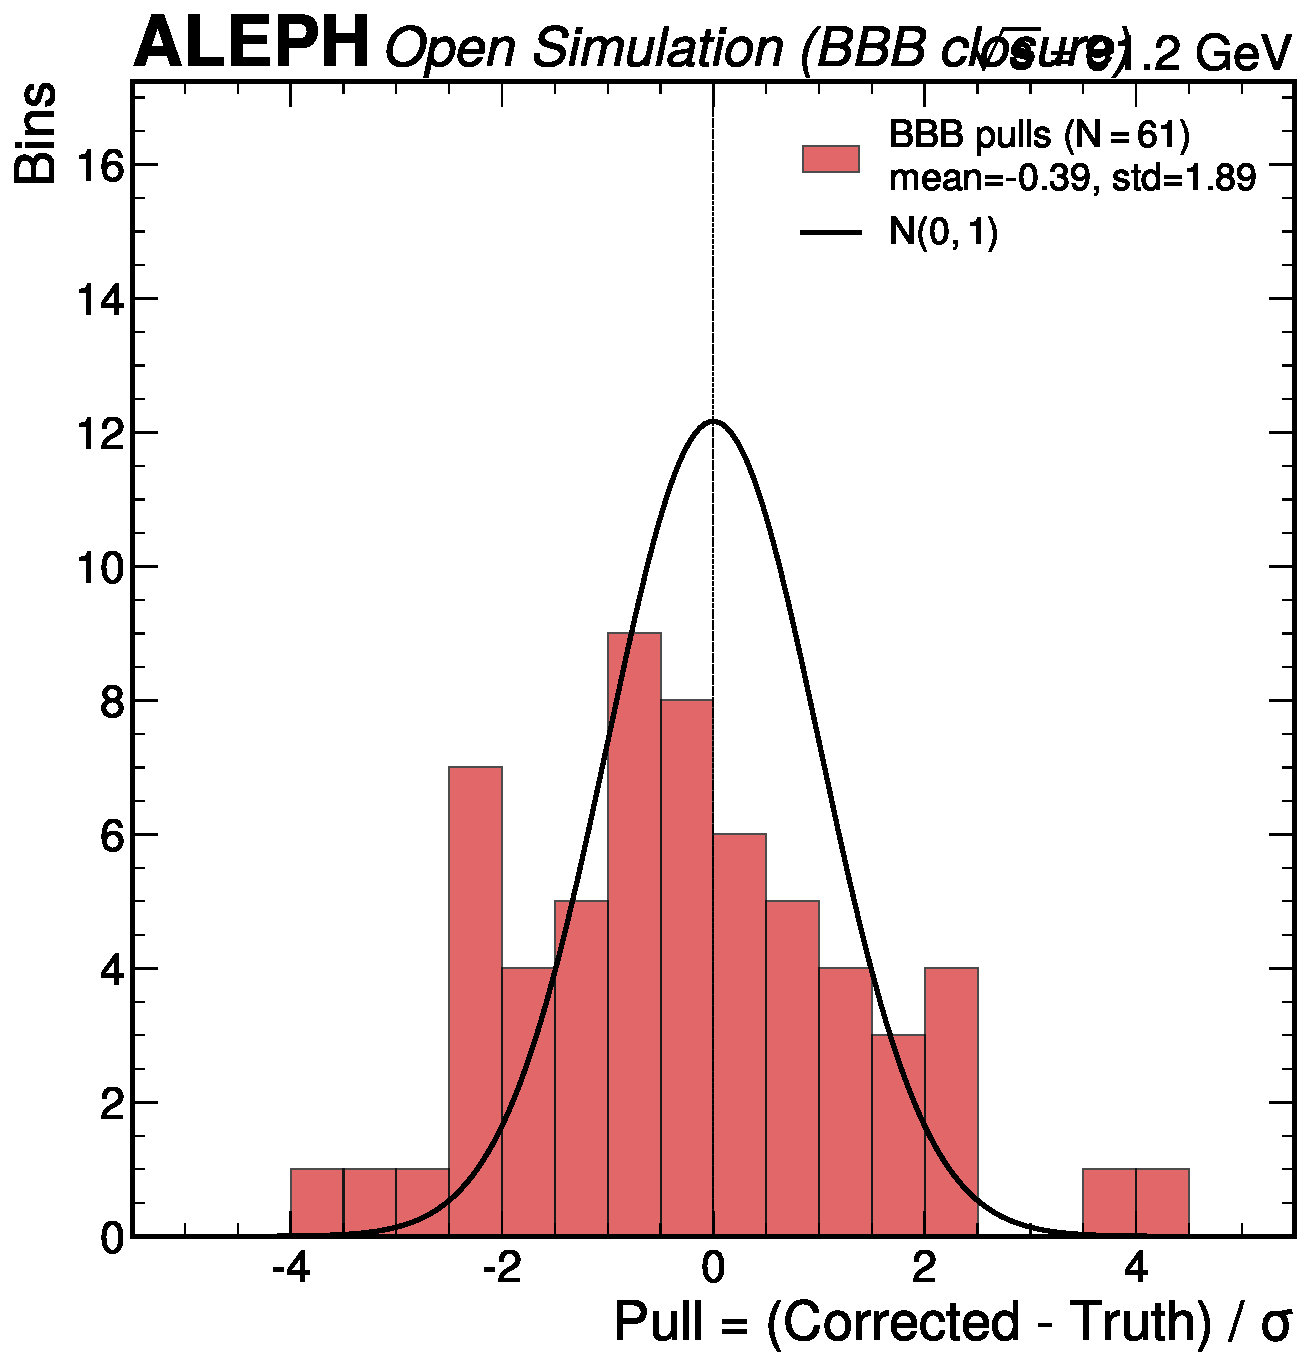
\includegraphics[width=0.47\linewidth]{figures/felix_closure_pulls_bbb.pdf}\hspace{1em}%
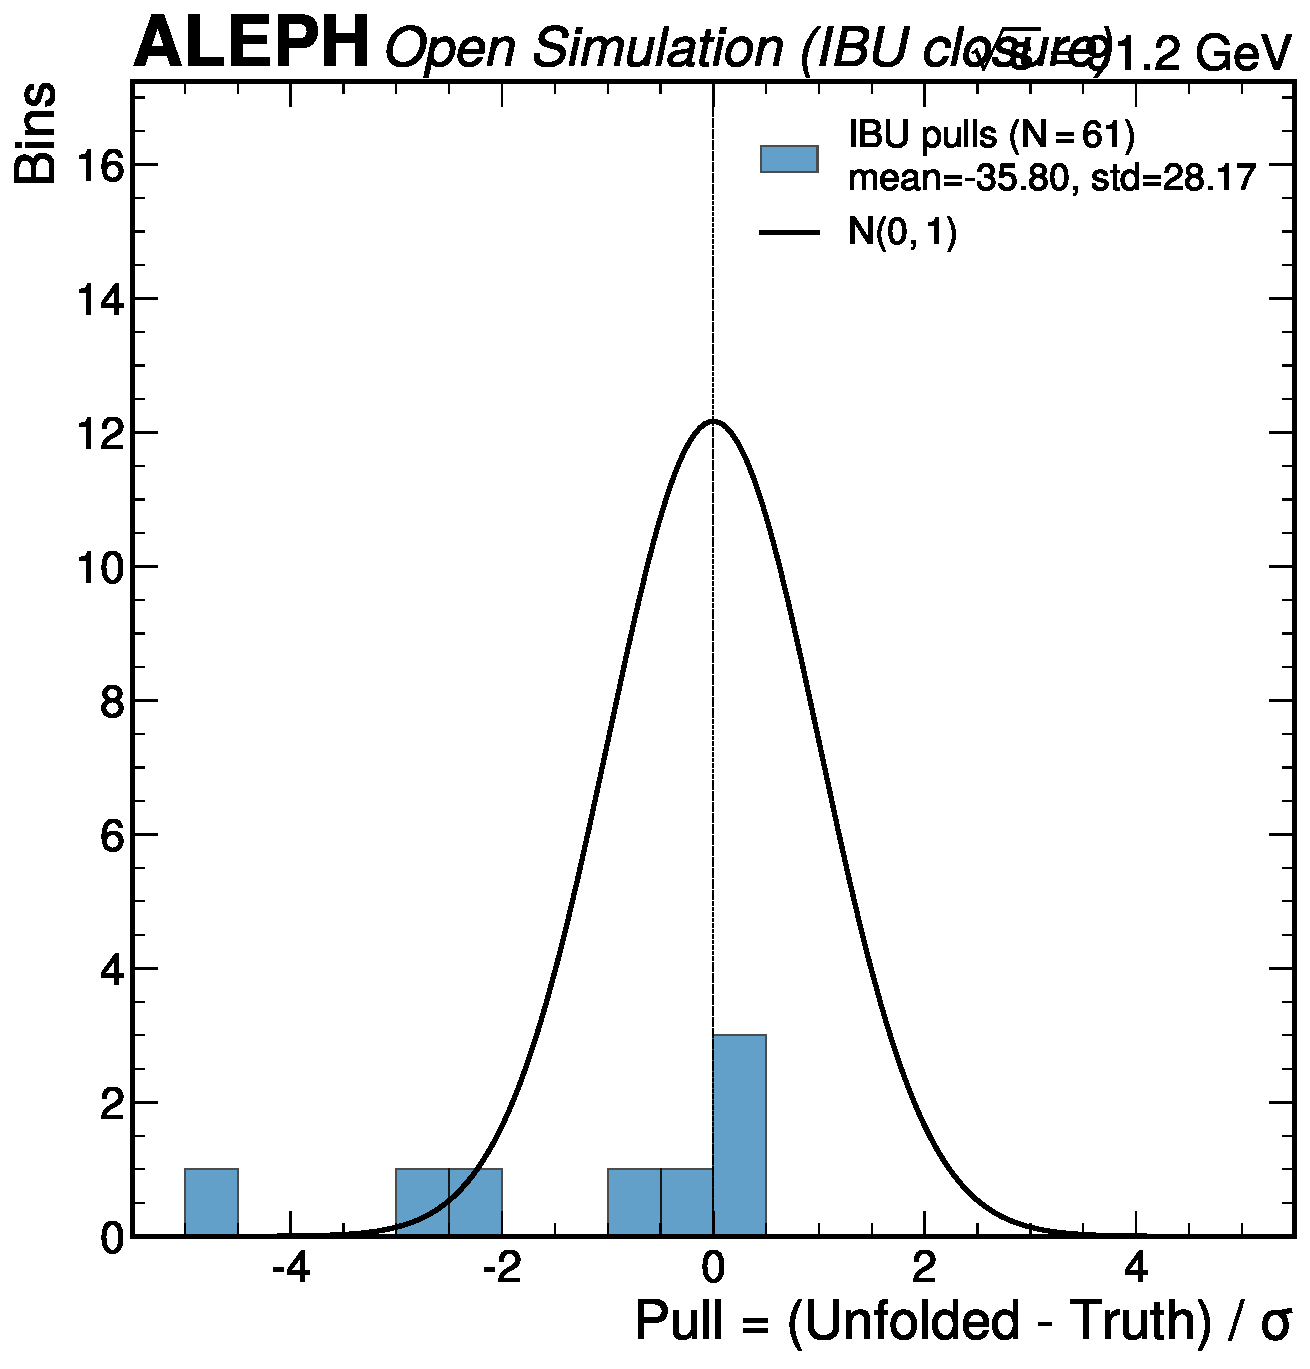
\includegraphics[width=0.47\linewidth]{figures/felix_closure_pulls_ibu.pdf}
\caption{Closure pull distributions from the Phase~4a initial
  computation (prior to split-sample re-analysis): BBB method (left)
  and IBU method (right).  The overlaid curve is $\mathcal{N}(0,1)$.
  Both were superseded by the updated analysis
  (Figure~\ref{fig:closure-pulls}), which includes bootstrap with
  full correction chain resampling.}
\label{fig:aux-closure-pulls}
\end{figure}

\begin{figure}[htbp]
\centering
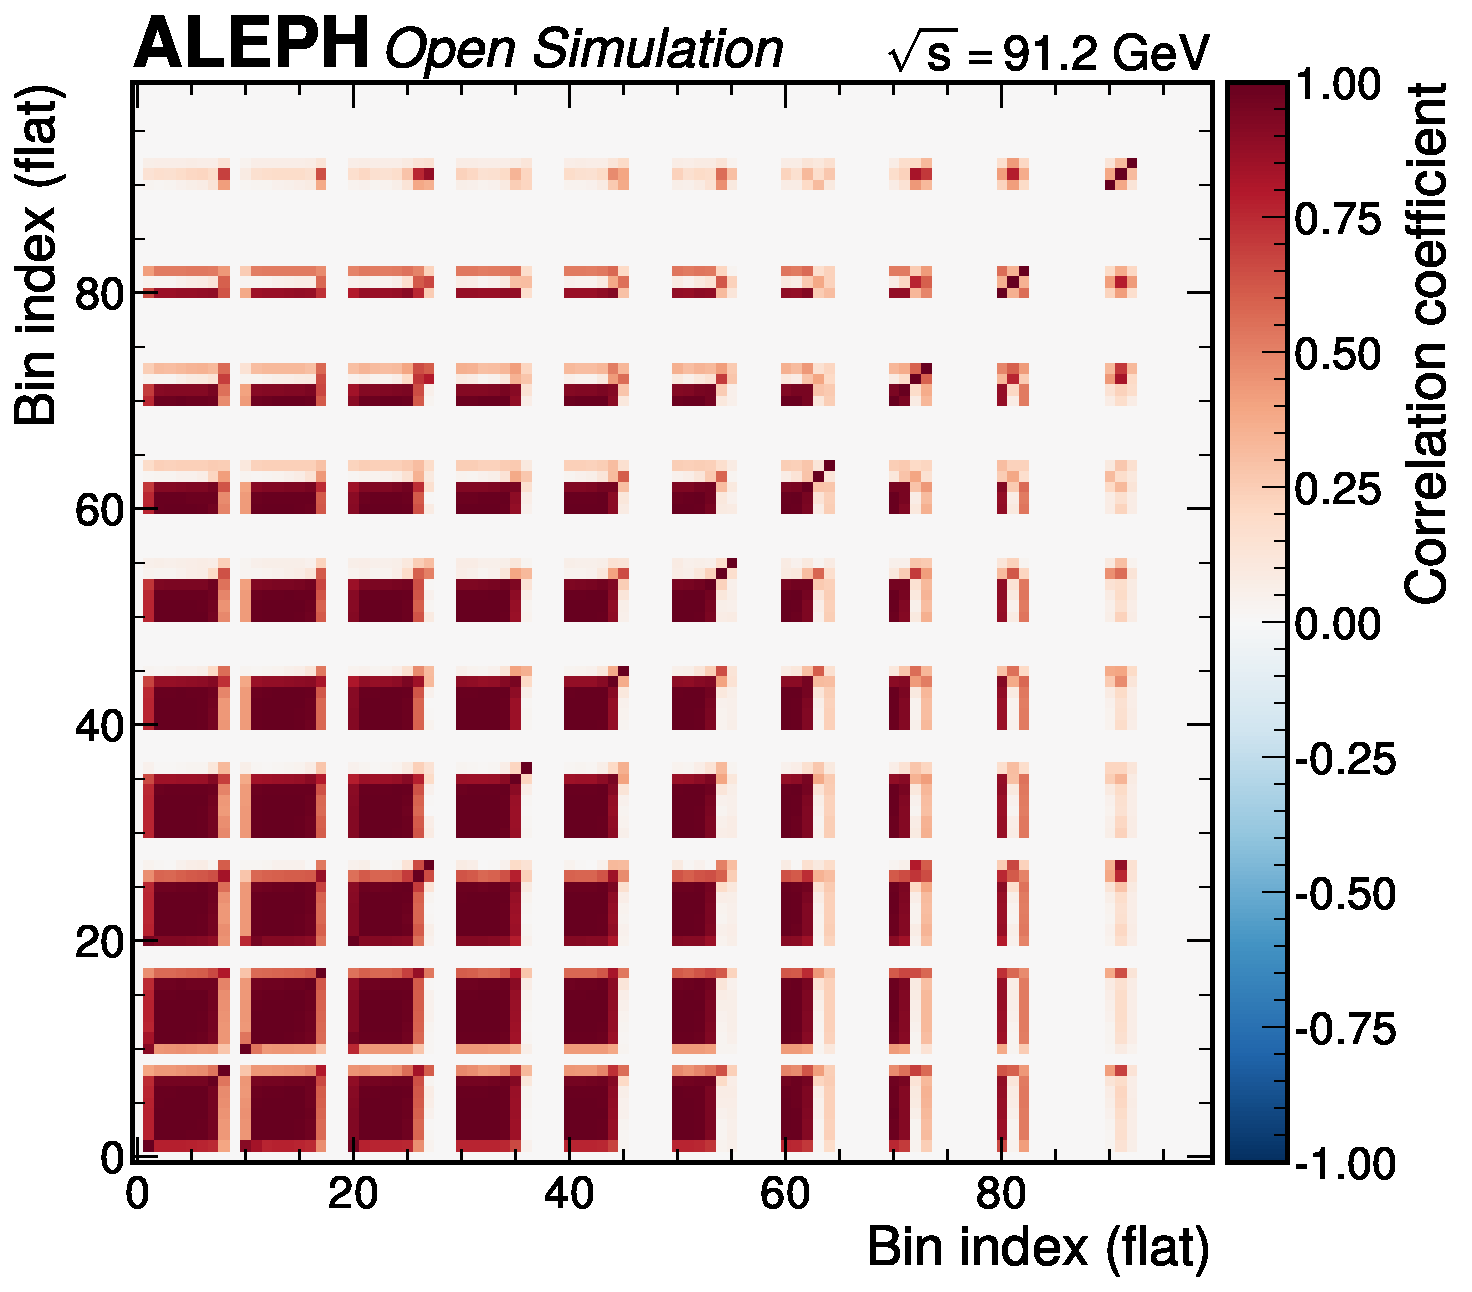
\includegraphics[width=0.55\linewidth]{figures/felix_correlation_matrix.pdf}
\caption{Correlation matrix from the Phase~4a initial computation.
  Superseded by Figure~\ref{fig:correlation-matrix}, which includes
  bootstrap with full correction chain resampling.}
\label{fig:aux-correlation}
\end{figure}

\begin{figure}[htbp]
\centering
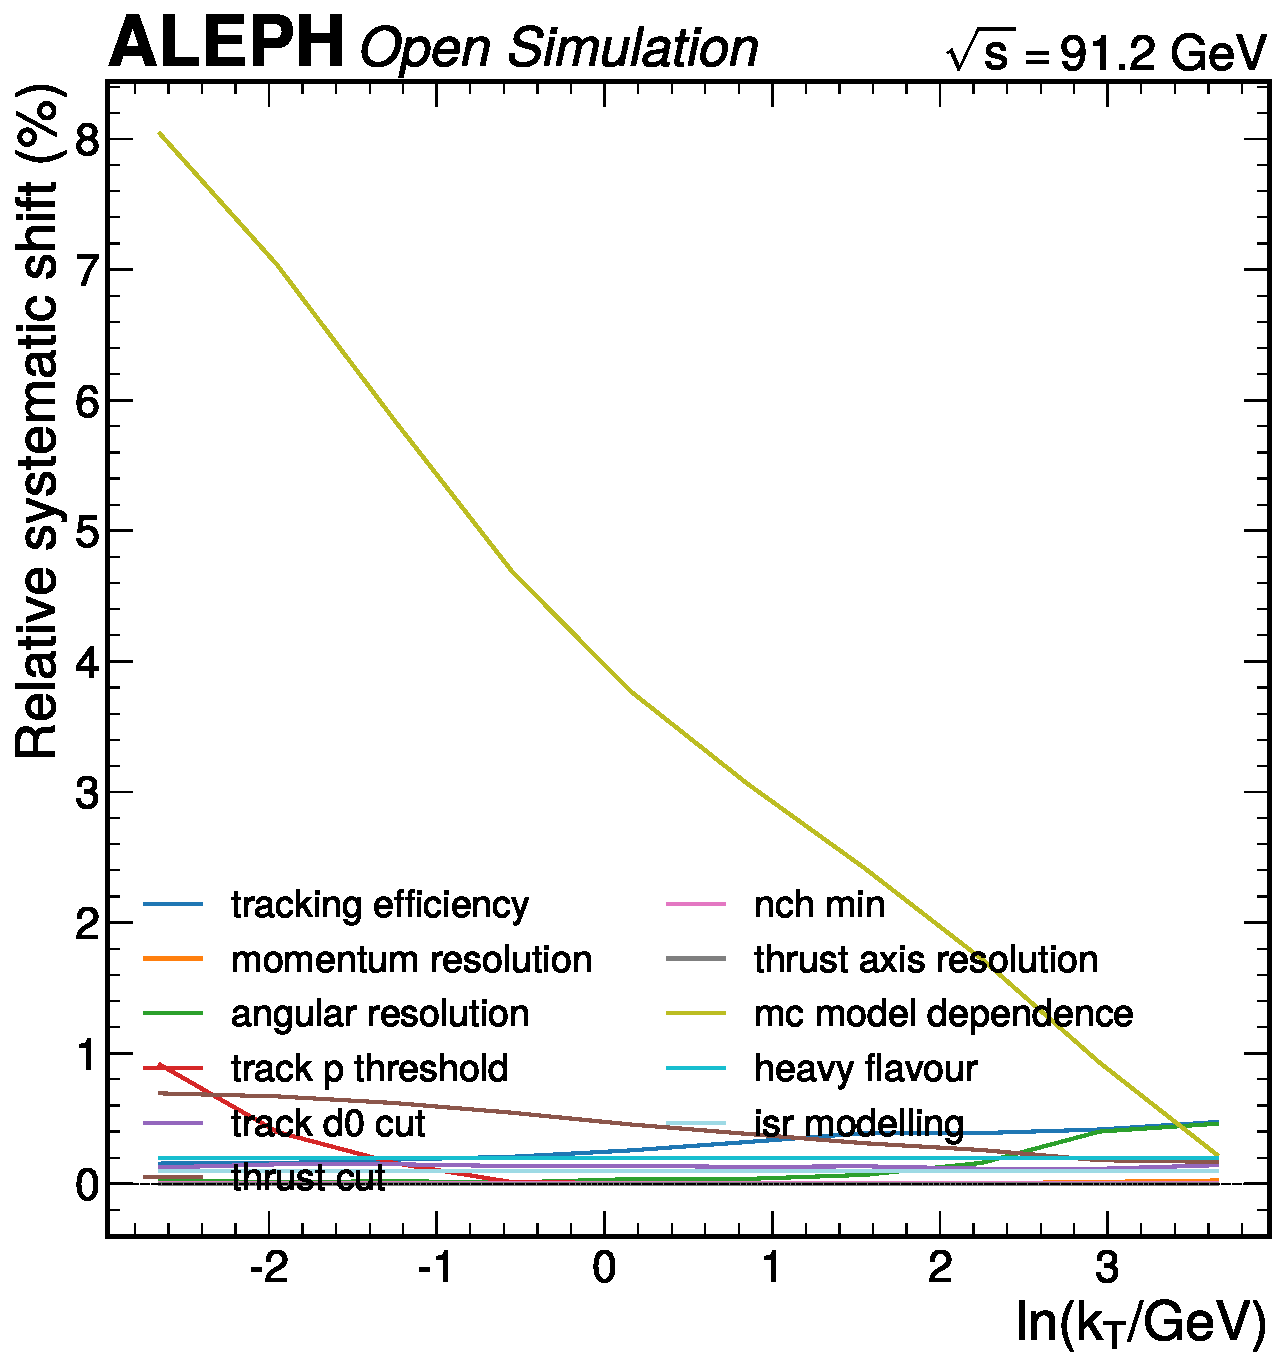
\includegraphics[width=0.47\linewidth]{figures/felix_syst_impact_kt.pdf}\hspace{1em}%
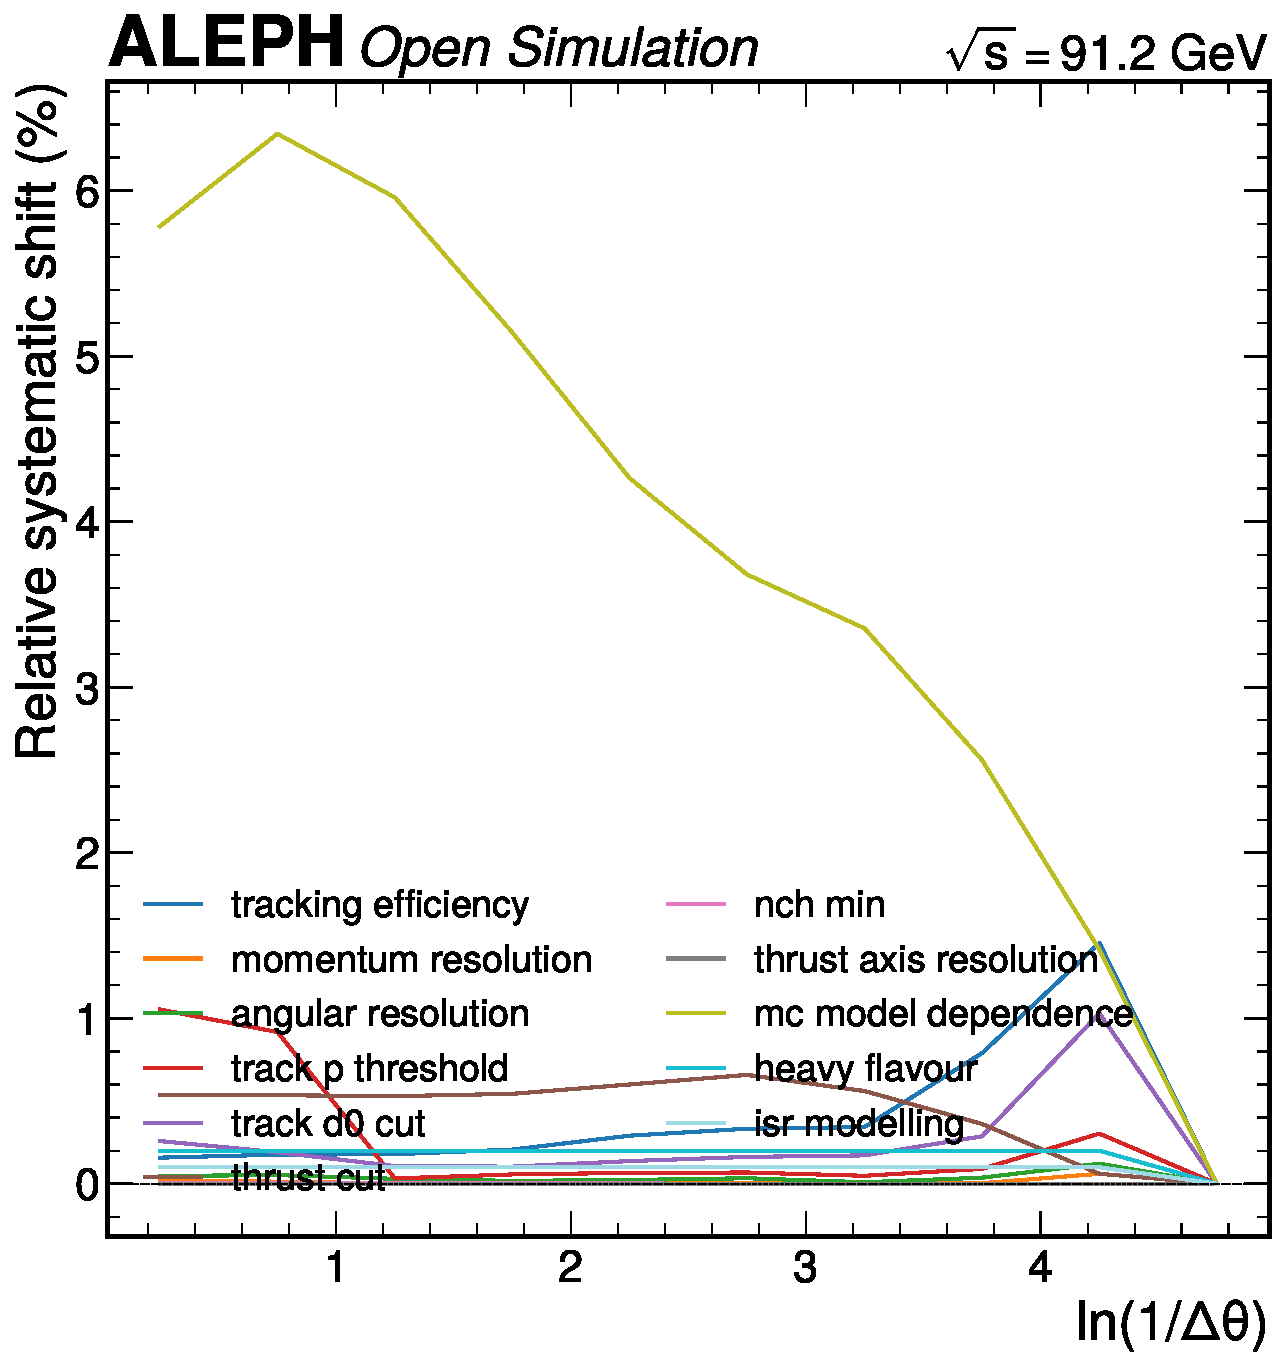
\includegraphics[width=0.47\linewidth]{figures/felix_syst_impact_dtheta.pdf}
\caption{Per-systematic impact on $\ln k_T$ (left) and
  $\ln(1/\Delta\theta)$ (right) projections from the initial
  Phase~4a computation (prior to removal of the IBU-vs-BBB systematic).
  The updated systematic impact plots
  (Figure~\ref{fig:syst-impact}) supersede these.}
\label{fig:aux-syst}
\end{figure}

\begin{figure}[htbp]
\centering
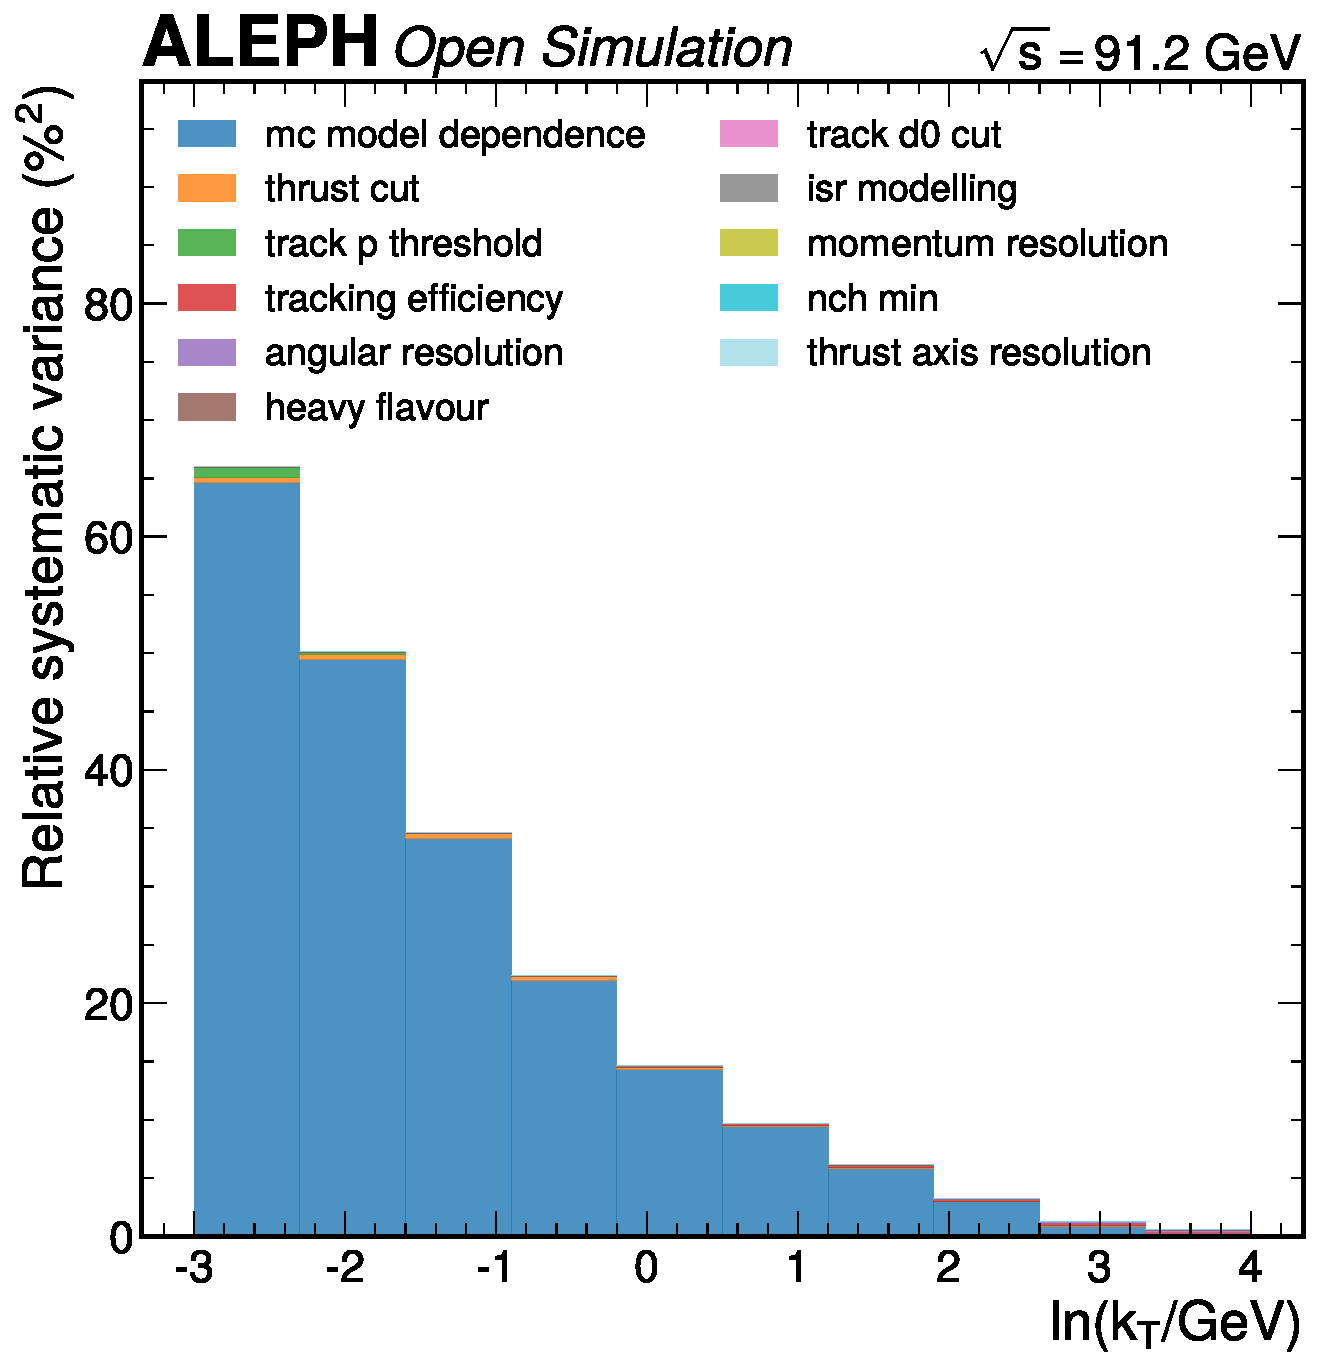
\includegraphics[width=0.47\linewidth]{figures/felix_syst_breakdown.pdf}\hspace{1em}%
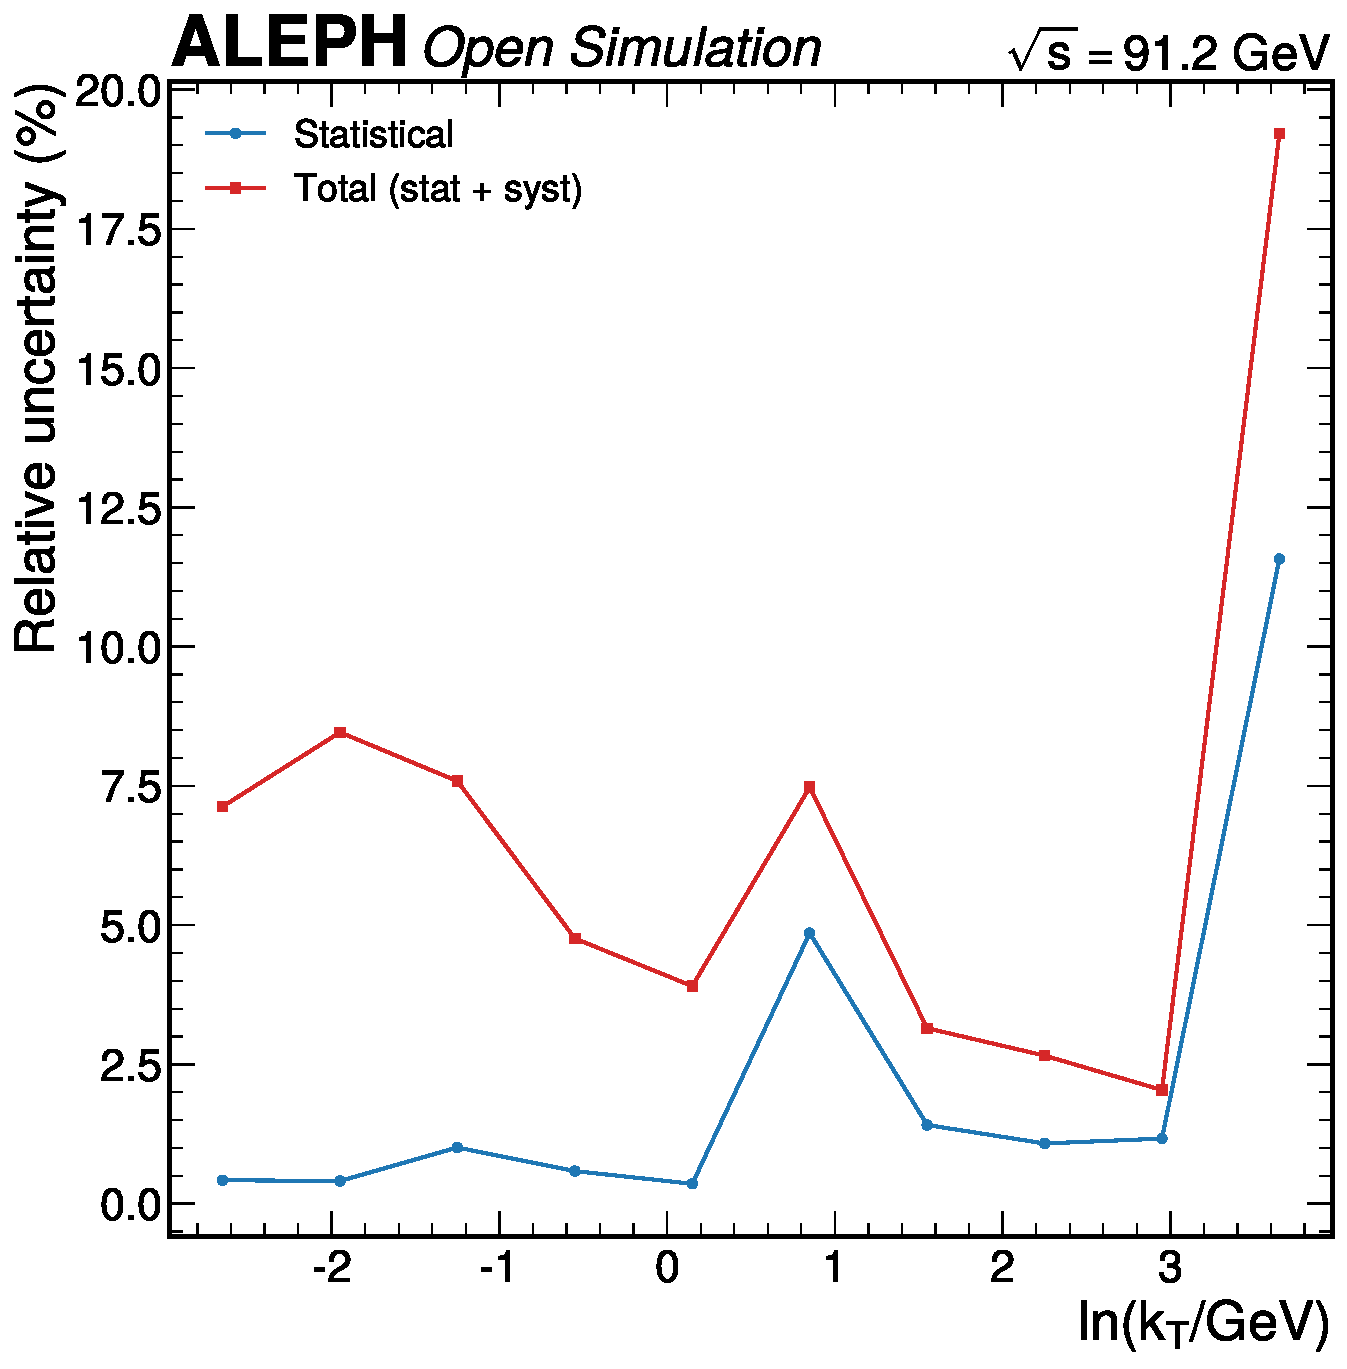
\includegraphics[width=0.47\linewidth]{figures/felix_uncertainty_summary.pdf}
\caption{Initial systematic breakdown (left) and uncertainty summary
  (right) from the Phase~4a initial computation.  Superseded by
  Figures~\ref{fig:syst-breakdown} and~\ref{fig:uncertainty-summary}.}
\label{fig:aux-syst-old}
\end{figure}

% =====================================================================
% E. LIMITATION INDEX
% =====================================================================
\section{Limitation Index}
\label{app:limitation-index}

Table~\ref{tbl:limitation-index} provides the complete registry of
constraints, limitations, and decisions from the analysis strategy,
together with their current implementation status.

\begin{table}[htbp]
\centering
\caption{Complete registry of constraints [A], limitations [L],
  and decisions [D] from the analysis strategy, with their current
  status.}
\label{tbl:limitation-index}
\begin{tabular}{llp{6cm}l}
\toprule
Label & Type & Description & Status \\
\midrule
{[A]} & Constraint & Particle-level: charged, $p > 200$~MeV/$c$,
  $c\tau > 1$~cm & Implemented \\
{[D1]} & Decision & C/A clustering for Lund plane & Implemented \\
{[D2]} & Decision & Primary declustering chain & Implemented \\
{[D3]} & Decision & $10 \times 10$ uniform binning & Implemented \\
{[D4]} & Decision & \texttt{pwflag == 0} (charged only) & Implemented \\
{[D5]} & Decision & Thrust cut $T > 0.7$ & Implemented \\
{[D6]} & Decision & MVA not used (no S/B needed) & Justified \\
{[D7]} & Decision & Durham 2-jets as Approach~C & Implemented \\
{[D8]} & Decision & BBB as co-primary correction & Primary \\
{[D9]} & Decision & IBU downscoped to cross-check & Downscoped \\
{[D10]} & Decision & ISR/FSR treatment & Implemented \\
{[D11]} & Decision & Bootstrap covariance, 500 rep. & Implemented \\
{[D12]} & Decision & Bin-level response matrix & Implemented \\
{[D13]} & Decision & $p_T$ ordering primary & Partial \\
{[D14]} & Decision & Sherpa comparison deferred & Deferred \\
{[L]} & Limitation & Luminosity from event count & Documented \\
{[L]} & Limitation & Single MC (PYTHIA~6.1) & Documented \\
{[L]} & Limitation & \texttt{ntpc} inaccessible & Documented \\
\bottomrule
\end{tabular}
\end{table}

% =====================================================================
% F. REPRODUCTION CONTRACT
% =====================================================================
\section{Reproduction Contract}
\label{app:reproduction}

The full analysis can be reproduced with the following sequence of
commands from the analysis root directory
(\texttt{analyses/lund\_jet\_plane/}):

{\small
\begin{verbatim}
pixi install           # Environment setup

# Phase 2: Exploration
pixi run py phase2_exploration/src/01_explore_data.py
pixi run py phase2_exploration/src/02_data_mc_comparison.py
pixi run py phase2_exploration/src/03_lund_plane_reco.py
pixi run py phase2_exploration/src/04_binning_optimization.py
pixi run py phase2_exploration/src/05_ordering_comparison.py

# Phase 3: Selection
pixi run py phase3_selection/src/01_apply_selection.py
pixi run py phase3_selection/src/02_correction_factors.py
pixi run py phase3_selection/src/03_closure_test.py
pixi run py phase3_selection/src/04_data_mc_lund.py
pixi run py phase3_selection/src/05_approach_comparison.py

# Phase 4a: Inference (expected)
pixi run py phase4_inference/4a_expected/src/01_corrected_lund.py
pixi run py phase4_inference/4a_expected/src/02_systematics.py
pixi run py phase4_inference/4a_expected/src/03_ibu.py
pixi run py phase4_inference/4a_expected/src/04_covariance.py
pixi run py phase4_inference/4a_expected/src/05_split_closure.py
pixi run py phase4_inference/4a_expected/src/06_stress_tests.py

# Phase 4b: Inference (10% data)
pixi run py phase4_inference/4b_partial/src/01_process_10pct.py
pixi run py phase4_inference/4b_partial/src/02_correct_10pct.py
pixi run py phase4_inference/4b_partial/src/03_compare_expected.py
pixi run py phase4_inference/4b_partial/src/04_per_year_stability.py

# Phase 4c: Inference (full data)
pixi run py phase4_inference/4c_observed/src/01_process_full_data.py
pixi run py phase4_inference/4c_observed/src/02_correct_and_compare.py
pixi run py phase4_inference/4c_observed/src/03_diagnostics.py
pixi run py phase4_inference/4c_observed/src/04_write_json.py

# Analysis note compilation (FINAL)
cd analysis_note && tectonic ANALYSIS_NOTE_doc4c_v3.tex
\end{verbatim}
}

\textbf{Data path:} The \texttt{.analysis\_config} file must contain
the path to the archived ALEPH data directory.  The 6 data files and
40 MC files total approximately 25~GB.

\textbf{Runtime estimate:} Phase~2: $\sim$5~min.  Phase~3: $\sim$30~min
(8-worker parallel processing).  Phase~4a: $\sim$45~min.  Total:
$\sim$1.5~hours on a modern multi-core machine.

\end{document}
